\documentclass [10pt, twoside] {uwthesis}[2012/04/02]

\usepackage[utf8]{inputenc}
\usepackage{amsmath}
\usepackage{amsfonts}
\usepackage{amssymb}
\usepackage{graphicx}
\usepackage{epstopdf}
\usepackage{lscape}
\usepackage{longtable}
\usepackage{afterpage}

\begin{document}
\setlength{\LTcapwidth}{9in}

\prelimpages
\Title{Reduced Limit on the Permanent \\ Electric Dipole Moment of $^{199}$Hg}
\Author{Brent M. Graner}
\Year{2017}
\Program{Department of Physics}

\Chair{Blayne R. Heckel}{Professor}{Department of Physics}
\Chair{Boris Blinov}{Professor}{Department of Physics}
\Signature{Leslie J. Rosenberg}

%\copyrightpage
\titlepage  
\setcounter{page}{-1}
\abstract{

This thesis describes an experiment to measure the permanent electric dipole moment (EDM) of $^{199}$Hg. The EDM is manifested as a small perturbation to the Larmor precession frequency due to the interaction energy of the electric dipole with a static electric field. The atoms are prepared in four separate glass vapor cells using optical pumping with resonant 254nm laser light and allowed to precess in a common magnetic field and oppositely-directed electric fields. The precession frequency difference in a pair of cells is derived from the accumulated phase difference between two probe periods separated in time. Using this technique, we find the $^{199}$Hg EDM projection onto the nuclear spin axis $d_{Hg} = (2.20 \pm 2.75_{stat} \pm 1.48_{syst}) \cdot 10^{-30} e\cdot \text{cm}$. While consistent with zero, this result places a new upper limit on the $^{199}$Hg EDM $|d_{Hg}| < 7.4\cdot 10^{-30} e\cdot \text{cm}$ (95\% C.L.), improving the previous best limit by a factor of $>4$. The new limit places stringent constraints on theories of physics beyond the Standard Model which incorporate new sources of time-reversal or $CP$ symmetry violation. This work was supported by NSF Grant No. 1306743 and the U.S. Department of Energy Office of Science, Office of Nuclear Physics under Award No. DE-FG02-97ER41020.}

\setcounter{tocdepth}{2}
\tableofcontents
\listoffigures
\listoftables
%\acknowledgments{First and foremost, I would like to acknowledge my colleagues on the Hg EDM experiment: Professor Blayne Heckel for providing critical guidance at every stage of the work, imposing some semblance of a plan on the rest of us, and showing three raw recruits how the project was done at a point when everyone else on the project had moved on; Scientific Glassblower Eric Lindahl, whose immense patience, deep knowledge, and exacting attention to detail in crafting the newest sets of vapor cells has made all our advancements possible; Jennie Chen, for her dedicated, hands-on assistance in building, dismantling, and rebuilding the apparatus more times than I care to think about; Dr. Nathan Kurz and Dr. Adam Klesczewski, who gave me the necessary understanding to work with the laser frequency doubling cavities and the confidence to tear open and fix all our other malfunctioning equipment.

%Secondly, I would be remiss if I failed to mention the many people whose shoulders this work stands upon: Professor Norval Fortson for originating the entire Hg EDM project; Professor Mike Romalis for creating the laser-based Hg EDM apparatus; the successive generations of graduate students whose work this thesis is a continuation of, including Prof. Steve Lamoreaux, Dr. James Jacobs, Prof. Clark Griffith, and Dr. Matthew Swallows.}
%\dedication{\begin{center}To all of my teachers\\(but especially Mom and Dad)\end{center}}
\textpages
\renewcommand{\floatpagefraction}{0.75}

\chapter{Introduction}     
This chapter provides an overview of some of the theoretical underpinnings that form the motivation for our experiment. The purpose behind the mercury electric dipole moment (EDM) experiment unfolds from consideration of time-reversal ($T$), charge conjugation ($C$), and parity inversion ($P$), and the various systems in which these operations alter the observable physics at work. In particular, the existence of a finite EDM in the ground state of the $^{199}$Hg atom directly violates $P$ and $T$ symmetry, and can be shown to violate the combined symmetry operation $CP$ through the $CPT$ theorem. In addition, the potential cosmological consequences of a non-null EDM measurement are briefly discussed, including a possible contribution to an \textit{a priori} explanation of the preponderance of matter over antimatter in the known universe.
%\section{Overview of fundamental symmetries in nuclear and particle physics}  
%\subsection{Parity symmetry and the weak interaction} %Lee & Yang, Wu et al. 
%\subsection{CP symmetry violation in neutral K mesons} %Landau, Fitch & Cronin
%\subsection{CP violation in B mesons}

\section{The strong CP problem} %theta_QCD, %axion hypothesis
All experiments performed to date are consistent with a strong interaction that preserves $CP$ symmetry exactly. However, the most general QCD Lagrangian contains a $CP$-violating term \begin{equation}\mathcal{L}^{CPV}=\theta_{QCD}\dfrac{\alpha_s}{16\pi}G^{\alpha}_{\mu\nu}\tilde{G}_{\alpha}^{\mu\nu}.\end{equation} with a phase angle $\theta_{QCD}$, the gluon field-strength tensor $G$, and its dual $\tilde{G}$. \textit{A priori,} we would expect the phase angle $\theta_{QCD}$ to be of order 1, yet such a prediction implies there exists a neutron EDM on the order of $10^{-15}-10^{-16} e\cdot \text{cm}$ \cite{1979_Baluni_nEDM_from_QCD} \cite{1979_Crewther_et._al._nEDM_from_QCD}, where 1 $e\cdot \text{cm}$ corresponds to an EDM generated by a charge of one electron displaced from the origin by a distance of 1 cm. This predicted value is some ten orders of magnitude larger than present experimental limits \cite{2006_ILL_nEDM}. Using these empirical limits, one can place an extremely small upper bound $\mid\theta_{QCD}\mid < 10^{-10}.$ There is currently no explanation for the 'unnaturally' small size of  $\theta_{QCD}$ that is supported by experimental evidence, a discrepancy that has come to be known as the \textit{strong $CP$ problem}. 

In 1977, a putative solution to the strong $CP$ problem was put forth by Peccei and Quinn, who suggested that the quark mass matrix $M$ couples to a new, Higgs-like scalar field $\phi_a$ with an initial $U(1)$ invariance and some non-zero vacuum expectation value $\langle\phi_a\rangle$. It can then be shown that the quark mass matrix acquires additional phases under changes in $\theta_{QCD}$. Under the Peccei-Quinn theory, $\langle\phi_a\rangle$ is obtained by minimizing a potential which is a function of $\theta_{QCD}$, and the additional fermion mass terms acquired from the coupling to $\phi_a$ act in such a way that the potential $V(\phi_a)$ is minimized at the point where $\theta_{QCD} = 0$ when the fermion masses are defined to be real-valued \cite{1977_Peccei_Quinn}. Immediately, Weinberg and Wilczek pointed out that since the initial symmetry of $\phi_a$ with respect to changes in $\theta_{QCD}$ is spontaneously broken, there must be an undiscovered Nambu-Goldstone boson, which Wilczek termed the \textit{axion} \cite{1978_Wilczek_axion}\cite{1978_Weinberg_axion}. 

Since there are stringent upper bounds on the hypothetical axion coupling to normal matter, axions or axion-like particles have also been identified as a potential dark matter candidate particle, and many experimental searches have been carried out to cover the axion mass/coupling parameter space \cite{2005_Rosenberg_axion_review}. To date, none has succeeded in making a positive discovery, and various precision-measurement experiments have been proposed using atomic and molecular systems to search for axion-like fields coupled to atomic nuclei by observing nuclear EDMs which oscillate at a frequency determined by the associated particle's rest mass \cite{2013_Graham_and_Rajendran_Direct_ALP_Detection, 2014_Budker_CASPEr_proposal, 2014_Flambaum_axion}. 

\section{CP violation and baryogenesis: the Sakharov conditions}
In addition to the Strong $CP$ problem, one of the major open questions in modern physics concerns the imbalance between matter and antimatter in the universe. In the absence of some symmetry-breaking mechanism, a universe created with equal amounts of matter and antimatter would have either left a universe of regions alternately dominated by one or the other, or annihilated perfectly, leaving behind much less matter density than is presently observed.\footnote{It is worth noting that the hypothesis of equal abundances of baryons and antibaryons at early times does not rest on any empirical observation, but on the prevailing theoretical bias towards a universe that began in a maximally-symmetric state and evolved according to laws which dynamically generated the observed asymmetries. The possibility remains that the baryon asymmetry was an initial condition of the universe, with no supporting \textit{a priori} reason.} The imbalance may be quantified by the parameter $\eta\equiv\dfrac{n_B-n_{\overline{B}}}{n_{\gamma}},$ where $n_B$ and $n_{\overline{B}}$ are the baryon and antibaryon densities, respectively, and $n_{\gamma}$ the photon density of the universe. Measurements using the Wilkinson Microwave Anisotropy Probe yielded a value $\eta=(6.14\pm0.25)\cdot10^{-10}$ \cite{ClineNotes}. Though it may appear small at first glance, this non-zero value of $\eta$ is far too \textit{large} to be accounted for with our current understanding of physics and cosmology. It was shown by A. Sakharov in 1967 that in order to dynamically generate a net asymmetry of baryons over antibaryons, three general conditions (now known as the \textit{Sakharov conditions}) must be met \cite{1967_Sakharov}: \begin{itemize}\item $B$-violating processes \item Additional sources of $CP$ violation \item Departures from thermal equilibrium in the early universe\end{itemize} Because EDM experiments constrain (or may discover) new sources of $CP$ violation, they are one of the primary experimental tests of baryogenesis models \cite{2010_EDM_Baryogenesis}. 

\section{EDMs and fundamental symmetries}
\subsection{Symmetry violation and EDMs of fundamental particles}
The original suggestion that an electric dipole moment would violate discrete symmetries is due to Ramsey and Purcell \cite{1950_Purcell_Ramsey_EDM}. In their 1950 work, they proposed testing the assumption of parity invariance for fundamental particles by measuring the EDM of the neutron (considered to be a fundamental particle at the time). According to their argument, a neutron EDM must be aligned with the particle's spin axis, as the spin is the only vector available to describe the system. In addition, the lack of additional degenerate energy states in a nuclear shell model implies that there is no need for an additional quantum number to specify the relative orientation of spin and EDM, as there can be only one value of the EDM projected onto the spin axis. Then, since the EDM is a ($P$-odd, $T$-even) polar vector, while the spin is a ($P$-even, $T$-odd) pseudovector, the scalar product of the two is odd under parity or time-reversal. This contradicts our previous point that the spin and EDM can only have one projection, and thus a non-zero EDM can be said to violate the discrete symmetries $P$, $T$, and $CP$ (the latter by way of the $CPT$ theorem). 
\begin{figure}
\begin{center}
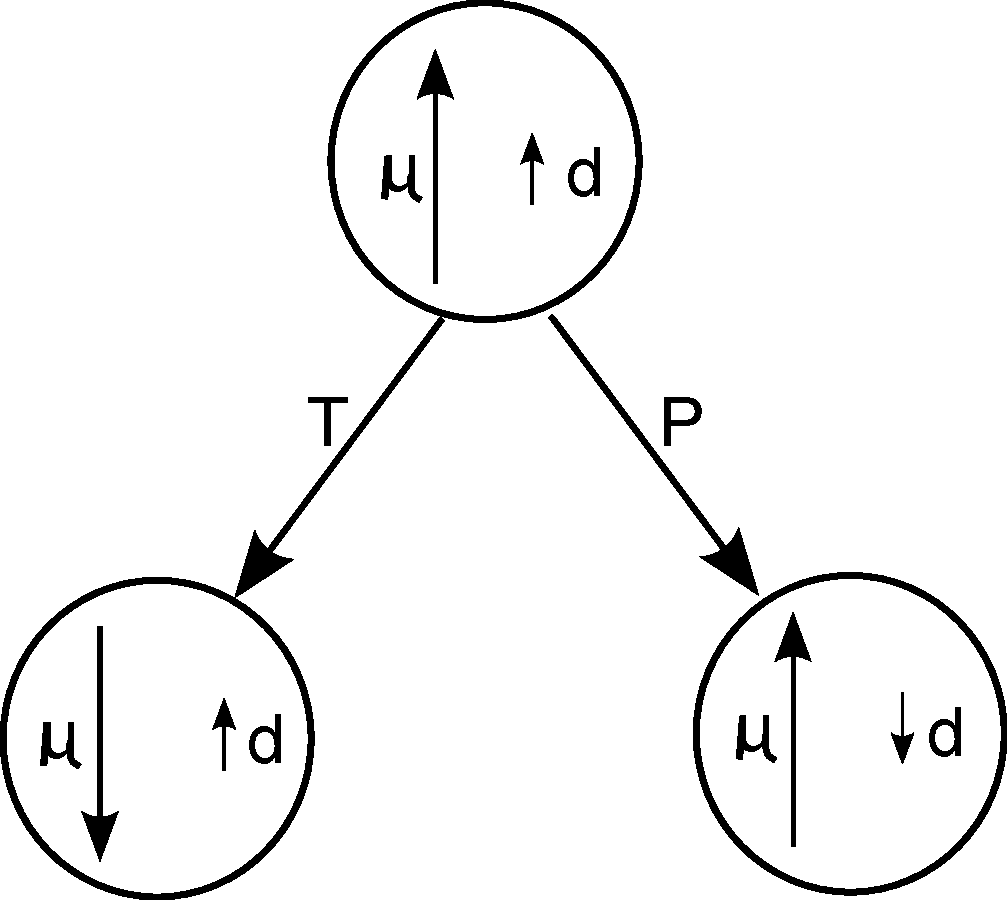
\includegraphics[scale=0.4]{Figures/EDM_polar_vector_P_T_violation.pdf}
\end{center}
\caption[Parity and Time-reversal symmetry violation with a polar vector EDM]%
{\narrower Symmetry violation in a fundamental particle with spin $\boldsymbol{\mu}$ and EDM $\mathbf{d}$. Because $\boldsymbol{\mu}$ and $\mathbf{d}$ have opposite transformation properties under parity ($P$) and time-reversal ($T$), and only one relative orientation can exist for any particle species, a $P$ or $T$ operation will transform the particle into a state that does not exist in nature. The existence of one preferred state of the symmetry operators shows that both parity and time-reversal symmetry are broken directly, without reference to the $CPT$ theorem.}
\label{polarvecPTv}
\end{figure}

The proposed neutron EDM experiment was carried out and results first published in \cite{1957_Smith_Purcell_Ramsey_nEDM}. The EDM was measured by passing a beam of polarized neutrons through an apparatus with uniform, static electric and magnetic fields $\mathbf{E}$ and $\mathbf{B}$, while $\pi/2$ pulses were applied by a pair of radio-frequency (RF) magnet coils arranged to measure the frequency of spin precession in the static $\mathbf{E}$ and $\mathbf{B}$ using the Ramsey method of separated oscillatory fields. When the projection of $\mathbf{E}$ onto $\mathbf{B}$ is changed, a nonzero EDM would cause the measured precession frequency to change as well. The experiment failed to resolve any such frequency shift, but was able to place an upper bound on the neutron EDM $|d_{n}| < 5\cdot 10^{-20} e\cdot \text{cm}.$ At the time, this result was one of the most precise measurements ever made, and yet in the intervening years it has been improved upon by more than six orders of magnitude \cite{2006_ILL_nEDM}.

Initially, the neutron was the sole focus of EDM experiments, despite the fact that stable atoms are technically much less challenging to work with. This was largely due to a simplified argument that a neutral atom cannot possess a permanent EDM. Beginning from considerations of parity in non-relativistic quantum mechanics, it can be shown that a bound state of multiple particles with no net charge cannot have a nonzero EDM in any non-degenerate eigenstate of a parity-invariant Hamiltonian \cite[p. 260]{Sakurai}. If an atom is considered as a set of electrons moving in a central potential created by the electrostatic interaction with the nuclear charge, then the parity eigenvalues of all the atomic states (neglecting spin) are given by the parity transformation properties of the spherical harmonic functions $Y^{\ell}_{m}(\theta,\phi)$: the parity eigenvalue is $-1^{\ell}$, where $\ell$ describes the total electronic orbital angular momentum. Since Hg exists in the ground state as a spin-singlet with $\ell = 0$, the ground state $\vert\alpha\rangle$ would be expected to have a parity eigenvalue $+1$: 
\[P\vert\alpha\rangle = \vert\alpha\rangle\] \[\langle\alpha\vert P^{\dagger}= \langle\alpha\vert.\] 
The electric dipole operator takes the form of a sum over all particles $\mathbf{D} = \sum_{i}q_i\mathbf{r}_i$, and it is manifestly odd under parity (since $P$ is defined to send $\mathbf{r}$ to $-\mathbf{r}$):
\begin{equation}\label{Dparity}P\mathbf{D} = -\mathbf{D}P \end{equation}
\begin{equation}\label{PD}\mathbf{D} = P^{\dagger}P\mathbf{D} = -P^{\dagger}\mathbf{D}P.\end{equation}
The EDM is the expectation value of $\mathbf{D}$ in state $\vert\alpha\rangle$: 
\begin{equation}\label{D=0}\langle\alpha\vert\mathbf{D}\vert\alpha\rangle = \langle\alpha\vert P^{\dagger}P\mathbf{D}\vert\alpha\rangle = -\langle\alpha\vert P^{\dagger}\mathbf{D}P\vert\alpha\rangle = -\langle\alpha\vert\mathbf{D}\vert\alpha\rangle,\end{equation}
and this relation can be satisfied only if the EDM vanishes.

\subsection{Schiff's Theorem and nonzero atomic EDMs} \label{Schiff_Moment}
More generally, we can relax some of the assumptions that lead to Eq. \eqref{D=0}, yet still end up with a vanishing atomic EDM. In particular, the \textit{Schiff theorem} states that any neutral system of point-like particles moving non-relativistically and having only electrostatic interactions must have zero EDM \cite{1963_Schiff}. This theorem holds regardless of any EDMs of the constituent particles, so no EDM of any fundamental particle or subset of particles within an atom can be observed by experimenting on the atom as a whole. Intuitively, Schiff's theorem describes the screening of a nuclear EDM by the electron cloud: if an experimenter places an atom with a nuclear EDM in an external electric field, the electron cloud will deform itself in such a way as to cancel the applied field at every point inside, thus preventing dipole interactions between the nucleus and the field produced in the lab \cite[Sec. 6.1]{Khriplovich_Lamoreaux}. At first glance, then, it would appear that any attempt to measure an EDM of a neutral atom is in vain. However, the conditions under which the Schiff theorem holds are all violated in atomic systems to varying degrees; electrons nearest a high-$Z$ nucleus can attain relativistic velocities, electronic fine structure and hyperfine interactions in the atom involve magnetic as well as electric forces, and the non-vanishing nuclear volume can contribute to effects which cause the electronic screening of a nuclear EDM to break down. For the case of diamagnetic atoms (atoms having zero electron angular momentum in the ground state), nuclear volume effects are expected to give the dominant contribution to the atomic EDM, and these contributions are therefore expected to increase with the number of nucleons \cite{2007_Liu_et._al._Schiff_Theorem_and_Corrections}.

\subsection{Nuclear moments leading to EDMs}
As shown in equation \eqref{D=0}, the parity-odd nature of the dipole operator $\mathbf{D} = \sum_{i}q_i\mathbf{r}_i$ forbids a non-zero EDM for any atomic state of definite parity, $\langle\alpha\vert\mathbf{D}\vert\alpha\rangle=0$. More generally, the inner product of $\mathbf{D}$ with any two parity eigenstates $\langle\alpha\vert\mathbf{D}\vert\beta\rangle=0$ unless they have opposite parity eigenvalues-the dipole operator only ``connects'' states of opposite parity. 

Therefore, in an atomic system, contributions to an EDM take the form of a product of expectation values for the normal dipole operator $\mathbf{D}$ and a $P$-odd, $T$-odd piece of the nuclear Hamiltonian $\mathbf{H}_{PT}$ \cite[eq. 123]{2004_Ginges_Flambaum_Fund._Symmetries_in_Atoms}: 
\begin{equation}\label{datom}
\mathbf{d}_{atom} = 2\sum_{\beta}\dfrac{\langle\alpha\vert\mathbf{D}\vert\beta\rangle\langle\beta\vert\mathbf{H}_{PT}\vert\alpha\rangle}{E_{\alpha}-E_{\beta}} = d_{atom}(\mathbf{F}/F),
\end{equation}
where $\vert\alpha\rangle$ is the ground state, $E_{\alpha,\beta}$ is the energy of state $\vert\alpha\rangle,\vert\beta\rangle$, and $\mathbf{F}$ is the ground state total angular momentum vector. 

It is important to point out that $d_{atom}$ is a scalar, so $\mathbf{d}_{atom}$ is a ($P$-even, $T$-odd) pseudovector proportional to the angular momentum of the ground state. This is in contradiction to the picture of symmetry violation given in \cite{1950_Purcell_Ramsey_EDM}, so our description of $P$ and $T$ violation for an atomic EDM must be revised. If an atom with spin magnetic moment $\boldsymbol\mu$ and EDM $\mathbf{d}$ is placed in an electric field $\mathbf{E}$ and a magnetic field $\mathbf{B}$, the Hamiltonian describing the interaction between the atom and the external fields is 

\begin{equation}\label{H}\mathbf{H} = -\boldsymbol\mu\cdot\mathbf{B} - \mathbf{d}\cdot\mathbf{E}.\end{equation}

Since $\boldsymbol\mu$ and $\mathbf{B}$ are both pseudovectors, their scalar product is invariant under $C$, $P$, $T$, or any combination thereof. By contrast, $\mathbf{d}$ is a pseudovector while $\mathbf{E}$ is a polar vector, so the term $\mathbf{d}\cdot\mathbf{E}$ is a pseudoscalar which is odd under $P$, $T$, or $CP$ (the latter following from the $CPT$ theorem). In this picture, the Hamiltonian describing the interaction with external applied fields is responsible for breaking the symmetry, while the previous argument (summarized in Figure \ref{polarvecPTv}), arrives at symmetry violation with the projection $\boldsymbol\mu\cdot\mathbf{d}$, which is a pseudoscalar if and only if $\mathbf{d}$ is a polar vector. While the polar vector EDM is the correct interpretation for experiments on more fundamental particles (e.g. electrons), it is not the case for the $^{199}$Hg EDM.
\begin{figure}
\begin{center}
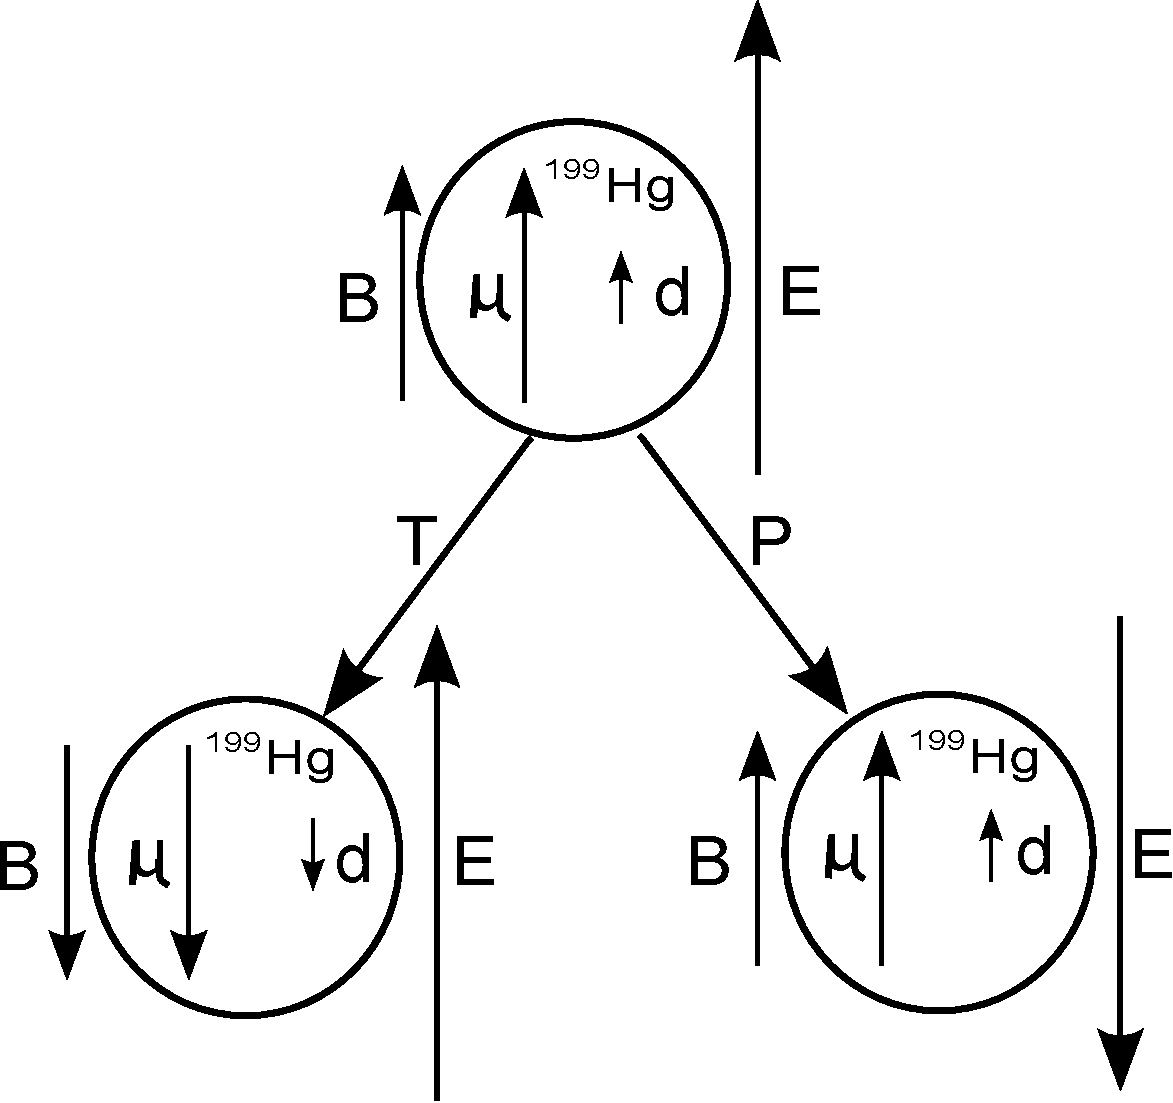
\includegraphics[scale=0.4]{Figures/EDM_pseudovector_P_T_violation.pdf}
\end{center}
\caption[Parity and Time-reversal symmetry violation with a pseudovector EDM]%
{\narrower Symmetry violation in the EDM Hamiltonian given by equation \eqref{H}. The relative orientation of $\mathbf{d}$ and $\boldsymbol{\mu}$ is constant under a parity transformation $P$ or time-reversal $T$, but the interaction of pseudovector $\mathbf{d}$ with polar vector $\mathbf{E}$ differs from the observed Hamiltonian in the parity transformed or time-reversed cases. When the precession between linear combinations of spin up and spin down states is observed, it follows that changing the relative orientation of $\mathbf{E}$ and $\mathbf{B}$ is physically equivalent to a $P$ or $T$ transformation.}
\label{pseudovecPTv}
\end{figure}

According to equation \eqref{datom}, to generate an atomic EDM there must exist some $P$-odd, $T$-odd part of the atomic Hamiltonian. In the case of $^{199}$Hg, the leading-order contribution comes from a contact interaction with a $P$-odd, $T$-odd nuclear moment referred to as the \textit{Schiff moment}, defined as \cite{2008_Schiff_Theorem_Rederivation}
\begin{equation}\label{SchiffMoment} 
\mathbf{S} = \dfrac{\mathbf{I}}{I} \dfrac{e}{10} \int \left( r^2 - \dfrac{5}{3} \langle r^2\rangle_{ch} \right) \mathbf{r} \rho(\mathbf{r})d^3r  \end{equation}
where $\langle r^2 \rangle_{ch}$ is the average of the squared radius of the nuclear charge distribution, $e$ is the proton charge, and $\rho(\mathbf{r})$ is the nuclear charge density, $\int \rho(\mathbf{r}) d^3\mathbf{r} = Z$.\footnote{The authors of \cite{2008_Schiff_Theorem_Rederivation} include a 'correction' term to the Schiff moment proportional to the mean value of the quadrupole moment of the nucleus, noting that this can only be non-zero for nuclei with spin $> 1/2$. Since the quadrupole term does not often appear as part of the Schiff moment elsewhere in the literature, and because $^{199}$Hg is a spin $1/2$ nucleus, this term has been dropped.} Because the Schiff moment is characterized by an integral over the nuclear volume, it must necessarily vanish in the limit of a point nucleus, thereby restoring Schiff's theorem prohibiting a non-zero atomic EDM.

It is also worth noting that the Schiff moment as defined above is independent of the EDM of any constituent nucleon(s). While there are additional terms proportional to nucleon EDMs that can be added to Eq. (\ref{SchiffMoment}), the dominant contribution to the Schiff moment depends only on the nuclear charge distribution \cite[Sec. 4.2]{2013_Engel_et_al_EDM_review}. It has been shown that T-odd, P-odd nucleon-nucleon interactions responsible for generating the charge distribution may induce a collective nuclear EDM two or three orders of magnitude larger than the standard model estimates of the neutron EDM \cite{1984_Sushkov_et._al._P_T_odd_atomic_experiments}. The contribution of this collective nuclear EDM $\mathbf{d}$ to the Schiff moment can be seen by re-casting Eq. (\ref{SchiffMoment}) to make the dependence explicit \cite{2004_Ginges_Flambaum_Fund._Symmetries_in_Atoms}:
\begin{equation}\label{dSchiffMoment} \mathbf{S} = \dfrac{\mathbf{I}}{I} \left[ \dfrac{1}{10}\int e\rho(\mathbf{r})\mathbf{r}r^2d^3r - \dfrac{1}{6}\dfrac{\mathbf{d}}{Z}\int \rho(\mathbf{r})r^2d^3r \right]. \end{equation}

Intuitively, one might expect that the nucleon EDM(s) simply add up to determine the nuclear EDM, which determines the atomic EDM in a straightforward fashion (up to some screening factor determined by the electron cloud re-arrangement). However, the conclusions above show that one must take a far more circuitous and counterintuitive path to arrive at a non-zero atomic EDM, where considerations of the Schiff moment are paramount. The nuclear theory behind the Schiff moment of $^{199}$Hg and the atomic theory relating it to the results described in this thesis are covered in more detail in chapter \ref{TheoryChapter}.

\section{EDMs in the Standard Model}
While $CP$ symmetry breaking in the strong interaction remains an open question, there is a $CP$-violating term in the CKM matrix which relates quark mass eigenstates to eigenstates of the weak interaction. This phase accounts for the $CP$-violating decay of neutral $K$ mesons to two pions \cite{1964_Fitch_Cronin_CP_violating_Kaon_Decay} as well as $CP$-violation observed more recently in experiments on $B$ mesons \cite{2001_Belle_B_meson_CP_violation, 2001_BaBar_B_meson_CP_violation}. Therefore, $CP$ is not a valid symmetry for all of nuclear physics, and it is possible to compute a Standard Model EDM which depends exclusively on the $CP$-violating CKM phase. However, quantitative estimates of Standard Model EDMs are many orders of magnitude smaller than present experimental limits. For example, the leading-order Standard Model contribution to the neutron EDM is estimated in \cite{2005_Pospelov_Ritz_EDM_review} at the level of $10^{-32} e\cdot\text{cm}$, approximately $10^6$ times smaller than the current experimental limit. While there CKM phase can induce nuclear or atomic EDMs, the magnitude of the effect is far too small to observe with experiments that are currently running or planned for the foreseeable future.

\begin{figure}
\begin{center}
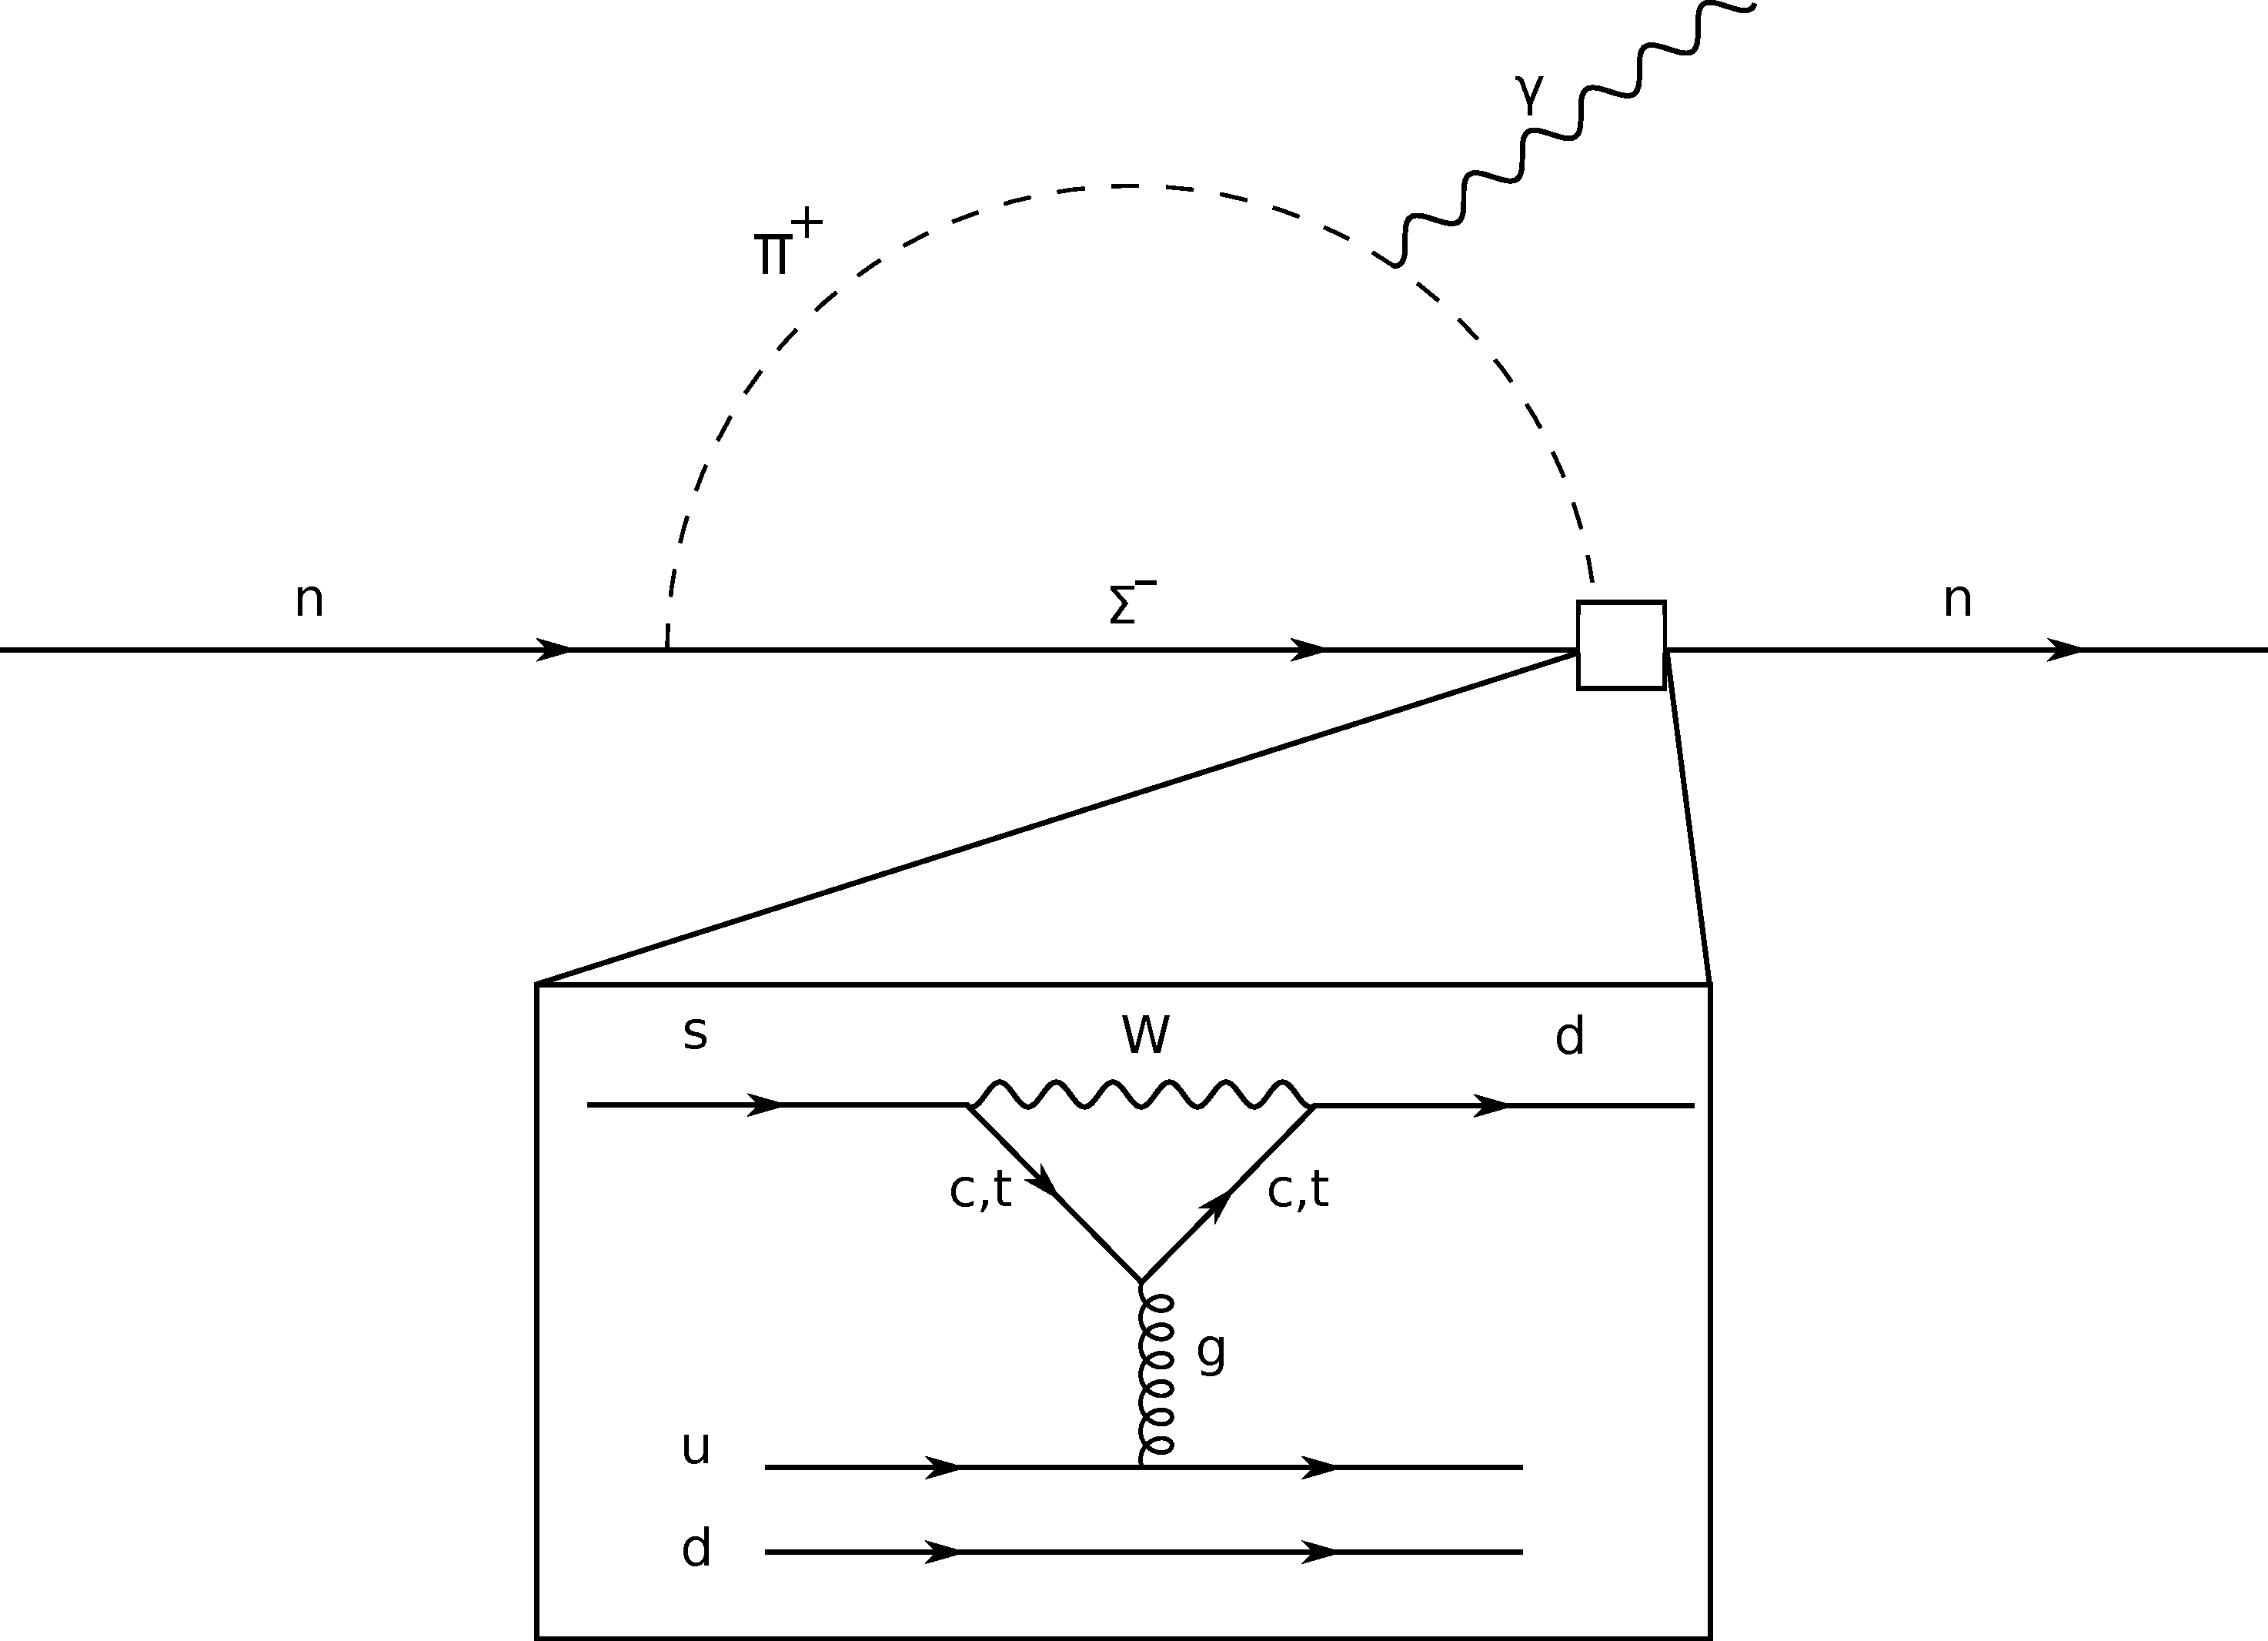
\includegraphics[scale=0.25]{Figures/SM_Neutron_EDM.pdf}
\end{center}
\caption[Leading-order neutron EDM contribution from Standard Model physics]%
{\narrower Feynman diagrams of the leading-order Standard Model contribution to a neutron EDM. The so-called ``penguin'' diagram involving the W-boson loop is embedded in the long-range pion loop illustrated on top. The full diagram is therefore at the two-loop level, suppressing the `bare' neutron EDM estimate to the level of $10^{-32} e\cdot\text{cm}$. Figure adapted from \cite{2005_Pospelov_Ritz_EDM_review}}
\end{figure}

\section{Summary of ongoing EDM experiments}
\subsection{Diamagnetic atom experiments} %Ra, Xe
Other experiments have measured the EDM of the $^{225}${R}a atom, recently reaching an upper limit $|d_{Ra}| < 5.0\cdot 10^{-22} e\cdot \text{cm}$ (95\% C.L.)\cite{2015_Ra_EDM}. The measurement was performed on a cloud of ultracold radium atoms loaded from a magneto-optic trap into a pair of crossed optical dipole traps within the magnetically-shielded region. The technical challenges facing this experiment (including the need for ultra-high vacuum and the $\sim$14 d half life of $^{225}${R}a) are substantial, but the EDM induced in the $^{225}${R}a nucleus by underlying $CP$-violating physics is expected to be enhanced by 2 to 3 orders of magnitude over that of the $^{199}${H}g nucleus \cite{1997_Spevak_et._al._EDM_enhancement}. The enhancement is due to the presence of a low-lying nuclear state with opposite parity from the ground state, which gives a large contribution according to Eq. \ref{datom} \cite{2013_Engel_et_al_EDM_review}. This enhancement effect means that the radium measurement can offer comparable sensitivity to new physics with less absolute precision than other experiments, and substantial improvements are expected with upgrades presently underway.

\subsection{Polar molecule experiments} %ThO, YbF, HfF
Experiments on polar molecules are primarily concerned with the EDM of the electron. The best current limit, set using a beam of ThO molecules, is $|d_{e}| < 8.7\cdot 10^{-29} e\cdot \text{cm}$ (90\% C.L.)\cite{2014_ACME_eEDM}. Polar molecules are advantageous in electron and semi-leptonic EDM searches because the internal electric fields are much stronger than any fields that can be externally applied; the ThO molecule has been found to be extraordinarily sensitive to an electron EDM with an 84 GV/cm effective field experienced by the electron between the thorium and oxygen nuclei, nearly seven orders of magnitude stronger than the applied field in the $^{199}$Hg experiment. A different polar molecule beam experiment using YbF found $|d_{e}| < 1.05\cdot 10^{-27} e \cdot \text{cm}$ (90\% C.L.)\cite{2011_YbF_EDM}. The $^{199}$Hg atom also has some sensitivity to an electron EDM through the coupling of nuclear and electron spins. Using our 95\% C.L. $|d_{Hg}| < 7.4\cdot 10^{-30} e\cdot cm$ and the relations $d_{Hg}\backsimeq 0.012 d_{e}$ \cite{1987_Martensson_Oster_eEDM} and $d_{Hg}\backsimeq -0.014 d_{e}$ \cite{1985_Flambaum_Khriplovich_eEDM_bound} gives an electron EDM limit $|d_{e}| < 5.7\cdot 10^{-28} e\cdot \text{cm},$ within an order of magnitude of the best polar molecule measurements. However, this limit carries some additional uncertainty given that the two calculations used provide an electron EDM of opposite sign for a given $^{199}$Hg EDM. 

\subsection{Ultracold neutron experiments} %PSI, Munich, Oak Ridge
This class of EDM experiments is perhaps most similar to the work described in this thesis. Because beam experiments are sensitive to motional magnetic fields $\mathbf{v} \times \mathbf{E}/c,$ current neutron EDM measurements are performed using ultra-cold neutrons (UCNs) produced in a reactor or accelerator beamline, then moderated and cooled below 4 K. UCNs can be stored similar to Hg atoms, and the UCN EDM experiments involve filling a neutron bottle with UCNs, transverse polarizing them with radio-frequency fields, then allowing them to precess for a fixed time in $\mathbf{E}$ and $\mathbf{B}$ fields, then reading out the phase of the Larmor precession by transmission through a magnetized foil. The current upper limit on the neutron EDM was initially reported as $|d_n| < 2.9 \cdot 10^{-26} e \cdot \text{cm}.$ (90\% C.L.) \cite{2006_ILL_nEDM}, but has since been increased to $3.0 \cdot 10^{-26} e \cdot \text{cm}$ due to identification of additional systematic effects \cite{2015_ILL_nEDM_gravity_correction}.\footnote{The \%95 C.L. result of \cite{2015_ILL_nEDM_gravity_correction} for the neutron EDM is $|d_n| < 3.6 \cdot 10^{-26} e \cdot \text{cm}.$} For purposes of comparison with the $^{199}$Hg EDM result, the neutron EDM upper limit set by our work is $1.6\cdot 10^{-26}$ $e\cdot\text{cm}$, approximately a factor of 2 better than the direct limit. However, our indirect limit rests on the assumption that the EDM of the unpaired `valence' neutron in the $^{199}$Hg nucleus is the sole contribution to the Schiff moment and the Schiff moment is itself the sole contribution to an atomic EDM.

\chapter{Atomic Interactions With Fields and Radiation: What the atoms are actually doing}
\section{EDM Hamiltonian and precession frequency}
The interaction Hamiltonian common to all EDM experiments was given in Eq. \eqref{H}:
\[\mathbf{H} = -\boldsymbol\mu\cdot\mathbf{B} - \mathbf{d}\cdot\mathbf{E}.\]
The first term describes the energy of interaction between the magnetic dipole moment $\boldsymbol\mu$ and the applied magnetic field $\mathbf{B}$, while the second term describes the analogous interaction between electric field $\mathbf{E}$ and EDM $\mathbf{d}$. If an EDM experiment is carried out on a two-level system, the energy splitting of the two magnetic sublevels is directly proportional to the precession frequency $\omega$:
$\hbar\omega = 2(\boldsymbol{\mu}\cdot\mathbf{B} + \mathbf{d}\cdot\mathbf{E}).$
Since $\mathbf{d}$ must always be parallel (or always antiparallel) to $\boldsymbol{\mu}$ for a given species \cite{Khriplovich_Lamoreaux}, and the EDM interaction is only a tiny perturbation to the magnetic interaction, this expression suggests a particularly simple experimental arrangement: measure the frequency of precession with an atom or particle in parallel $\mathbf{E}$ and $\mathbf{B}$ fields to get $\omega_+ = 2 (\boldsymbol{\mu}\cdot\mathbf{B} + \mathbf{d}\cdot\mathbf{E})/\hbar$, then flip the fields to antiparallel and measure $\omega_- = 2(\boldsymbol{\mu}\cdot\mathbf{B} - \mathbf{d}\cdot\mathbf{E})/\hbar$. The difference of the two precession frequencies is then \[\omega_+ - \omega_- = \dfrac{4\mathbf{d}\cdot\mathbf{E}}{\hbar}.\]

\section{Transverse optical pumping}
The Hg spins are prepared using left-handed ($\sigma_+$) circularly-polarized laser light resonant with the $^1$S$_0\rightarrow^3$P$_1$ transition, as shown in Figure \ref{OpticalPump}. Defining the light propagation vector $\mathbf{k}$ as the quantization axis, the light excites atoms into the $m_F=+1/2$ state of the F $=1/2$ hyperfine level, which can then decay to either ground state sublevel. However, angular momentum conservation prohibits absorption of $\sigma_+$ photons from the $m_F=+1/2$ ground state sublevel into the F $=1/2$ excited state level, and the light is approximately 20 GHz detuned from the F $= 1/2 \rightarrow $F $= 3/2$ transition frequency, so the ground state $m_F=+1/2$ sublevel is 'dark' to the laser light. Atoms are thus pumped into this state, while the population of the $m_F=-1/2$ sublevel of the ground state is depleted. 
\begin{figure}
\begin{center}
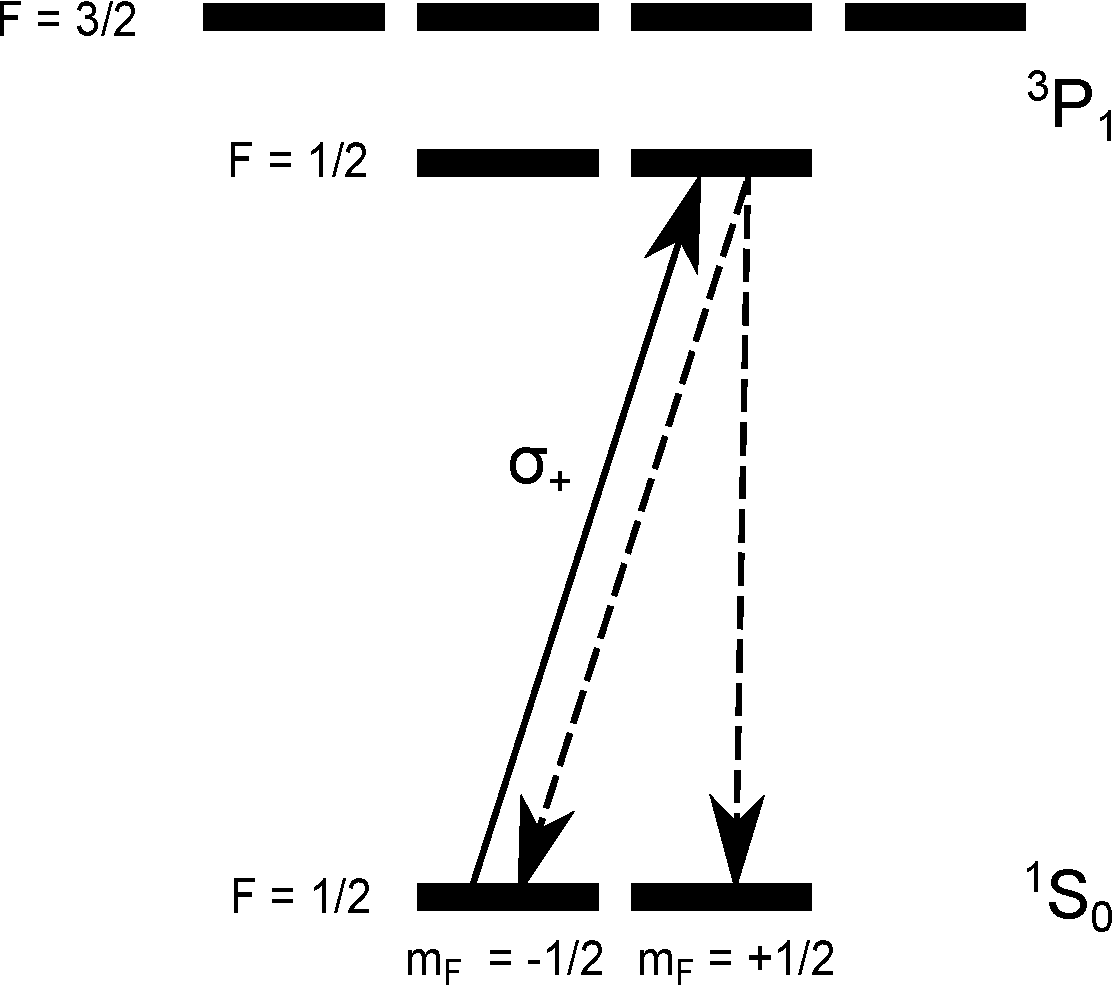
\includegraphics[scale=0.4]{Figures/Level_diagram.pdf}
\end{center}
\caption[Optical pumping diagram for F = 1/2]%
{\narrower A simplified level diagram of optical pumping on the $^1$S$_0\rightarrow^3$P$_1$ transition in $^{199}$Hg. Atoms are pumped into the $m_F=+1/2$ sublevel of the ground state, where the light propagation vector $\mathbf{k}$ defines the quantization axis. An intermediate metastable ($^3$P$_0$) state is not shown.}
\label{OpticalPump}
\end{figure}

Once atoms are pumped into the ground state $m_F=+1/2$ sublevel, they begin to precess about the transverse magnetic field. This can be seen most easily by a change of basis states so that the quantization axis points along the magnetic field $B_0$. In this new basis, we can write the wavefunction of the polarized atoms as $\vert\alpha\rangle = a(t)\vert+\rangle + b(t)\vert-\rangle$, where $a(t)$ and $b(t)$ are the time-dependent coefficients of the spin up and down eigenstates of the Hamiltonian $\vert+\rangle$ and $\vert-\rangle$. Neglecting the energy perturbation due to an EDM, we can write $\mathbf{H}$ in matrix form:
 \[ \mathbf{H} = \mu B_z \sigma_z = \mu B \begin{pmatrix} 1 & 0 \\ 0 & -1 \end{pmatrix} .\]
Solving the Schr\"{o}dinger equation for $a(t)$ and $b(t)$ gives the time evolution of a general superposition of eigenstates, 
\[\vert\alpha\rangle = a_0 e^{-i \mu B t /\hbar}\vert+\rangle + b_0 e^{i \mu B t /\hbar}\vert-\rangle.\]  
Since the atoms are initially polarized orthogonal to the magnetic field, we can represent the initial state $a_0\vert+\rangle + b_0\vert-\rangle$ as an eigenstate of 
\[\sigma_x =  \begin{pmatrix} 0 & 1 \\ 1 & 0 \end{pmatrix} .\]
which will be satisfied if $a_0 = b_0 = 1/\sqrt{2}$. Then, taking the time-dependent expectation value of $\sigma_x$, we obtain \[\langle\alpha\vert \sigma_x \vert\alpha\rangle = \dfrac{1}{2} e^{-2 i \mu B t /\hbar}  + \dfrac{1}{2} e^{2 i \mu B t /\hbar} = \cos(2 \mu B t /\hbar),\]
which gives the unperturbed Larmor frequency $\omega = 2 \mu B/\hbar.$ Since each atom begins to precess immediately once it is polarized, the pump light must be intensity-modulated ('chopped') in sync with the Larmor frequency in order to coherently build up a large polarization.

\section{Faraday rotation}
Once the atoms are pumped into the $m_F=+1/2$ sublevel and precessing about $B_0$, the laser light is changed to linear polarization by removing a $\lambda/4$ waveplate from the beam. As the light propagates through the Hg vapor cell, it can experience a phase shift due to the index of refraction of the atomic sample. For a monochromatic light source, the index of refraction $\eta(\omega)$ near an allowed transition can be written approximately as
\begin{equation} \label{eta}\eta(\omega) \approx 1 + 2\pi\chi_0\dfrac{\gamma_0}{2(\omega-\omega_0)+i\gamma_0}\end{equation}
where $\omega$ is the angular frequency of the light, $\omega_0$ is the frequency of the transition, $\gamma_0$ is the natural line width, and $\chi$ is the atomic susceptibility \cite{Kimball}. Note that the index of refraction can also be shifted differently for different polarization states, so that the sample acquires birefringence as a result of the polarization.\footnote{For a thorough treatment of linear and non-linear magneto-optical rotation, including a discussion of Faraday's original experiments, see \cite{Kimball}.} 

\begin{figure}
\begin{center}
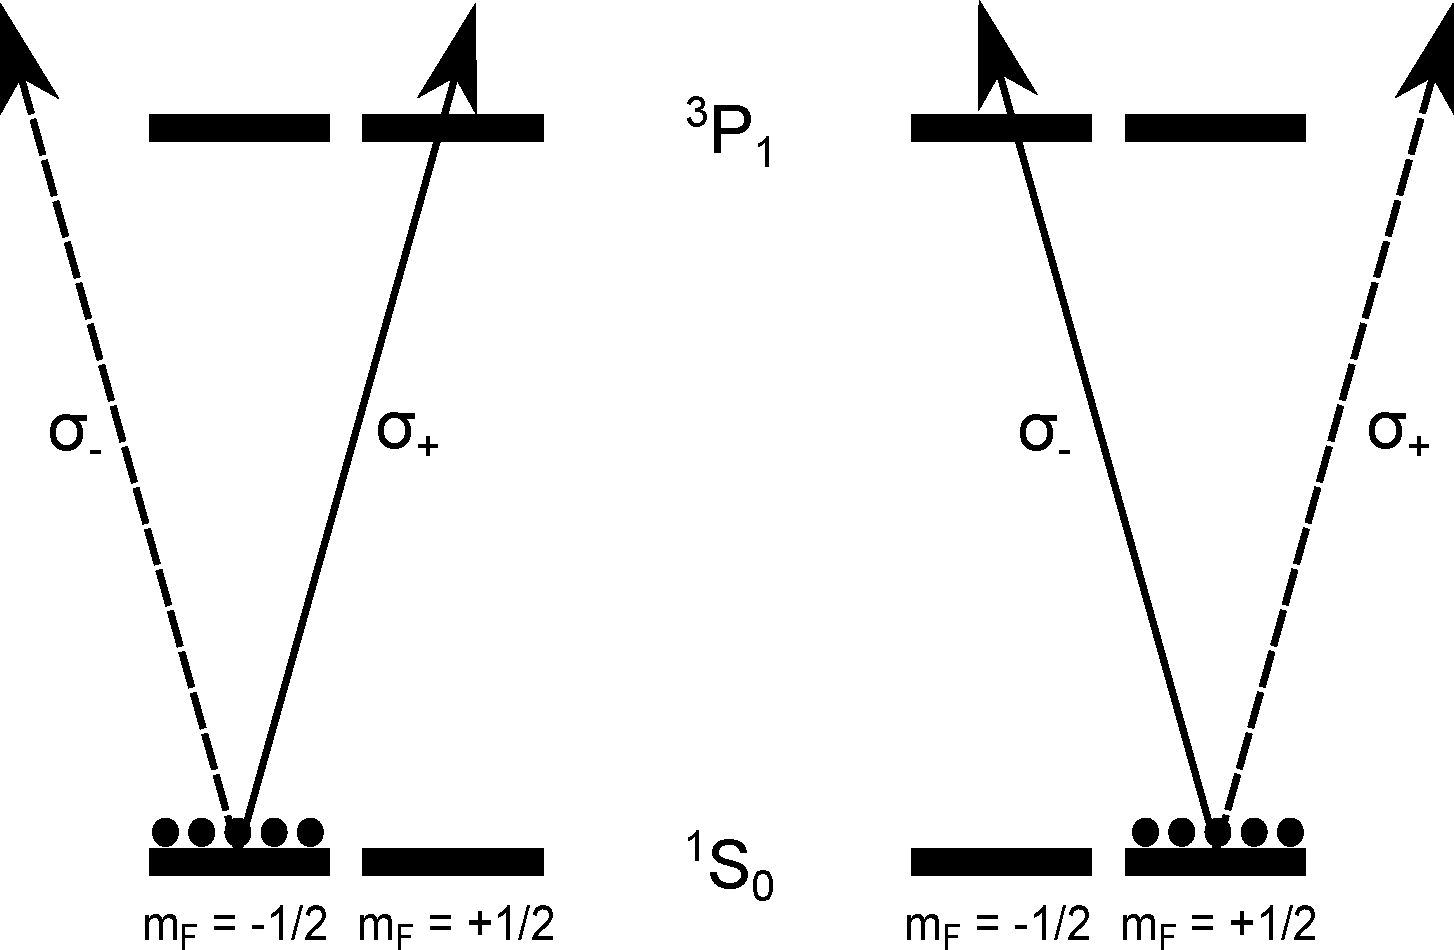
\includegraphics[scale=0.4]{Figures/Faraday_rotation.pdf}
\end{center}
\caption[Faraday rotation of polarized atoms]%
{\narrower A schematic diagram of Faraday rotation for a non-equilibrium sample of precessing atoms interacting with radiation near an F = 1/2 $\rightarrow$ F = 1/2 transition. Left: When the ensemble of atoms is polarized in the $m_F=-1/2$ sublevel, the $\sigma_+$ component of the beam is near (+10 GHz detuned from) an allowed transition, enhancing the index of refraction for $\sigma_+$ relative to $\sigma_-$. Right: one half-period later, atoms are polarized in the $m_F=+1/2$ sublevel, enhancing the index of refraction for the $\sigma_-$ beam component. The quantization axis is defined here to be the axis of light propagation.}
\label{FaradRot}
\end{figure}

In the case of the precessing Hg spins, the atomic population cycles between the degenerate $m_F=+1/2$ and $m_F=-1/2$ states in the basis defined by the laser light propagation axis. For light near an $F = 1/2 \rightarrow F = 1/2$ transition, one circular polarization state is near an allowed transition whenever the atoms are in a pure state (either parallel or antiparallel to the light beam), while the other polarization component is not. The small phase shift in the $\sigma_+$ vs. $\sigma_-$ components of the beam will cause the output light polarization axis to rotate from that at the input by an amount proportional to the degree of atomic polarization. As the atoms precess between the two states, the output light polarization will oscillate back and forth at the Larmor frequency, and as the atomic polarization decays back to equilibrium, the maximum angle of rotation will gradually become smaller with a characteristic lifetime that varies from cell to cell. The degree of polarization rotation depends on the projection of the atomic magnetization vector $\mathbf{M}(t)$ and the light propagation vector $\mathbf{k}$. The angle of polarization rotation can be described by the equation $\zeta(t) = A\theta e^{-t/\tau},$ where $\theta(t) = \cos(\omega t + \phi)$ is the angle between $\mathbf{M}$ and $\mathbf{k}.$ The amplitude coefficient $A$ is set by the degree of atomic polarization and the optical depth of the cell, and the coherence lifetime $\tau$ depends on the condition of the cell. A discussion of the factors which influence the lifetime $\tau$ is given in Chapter \ref{CellChap}.

\section{Precession with $\mathbf{B}_0 \cdot \mathbf{k} \neq 0 $}
\begin{figure}
\begin{center}
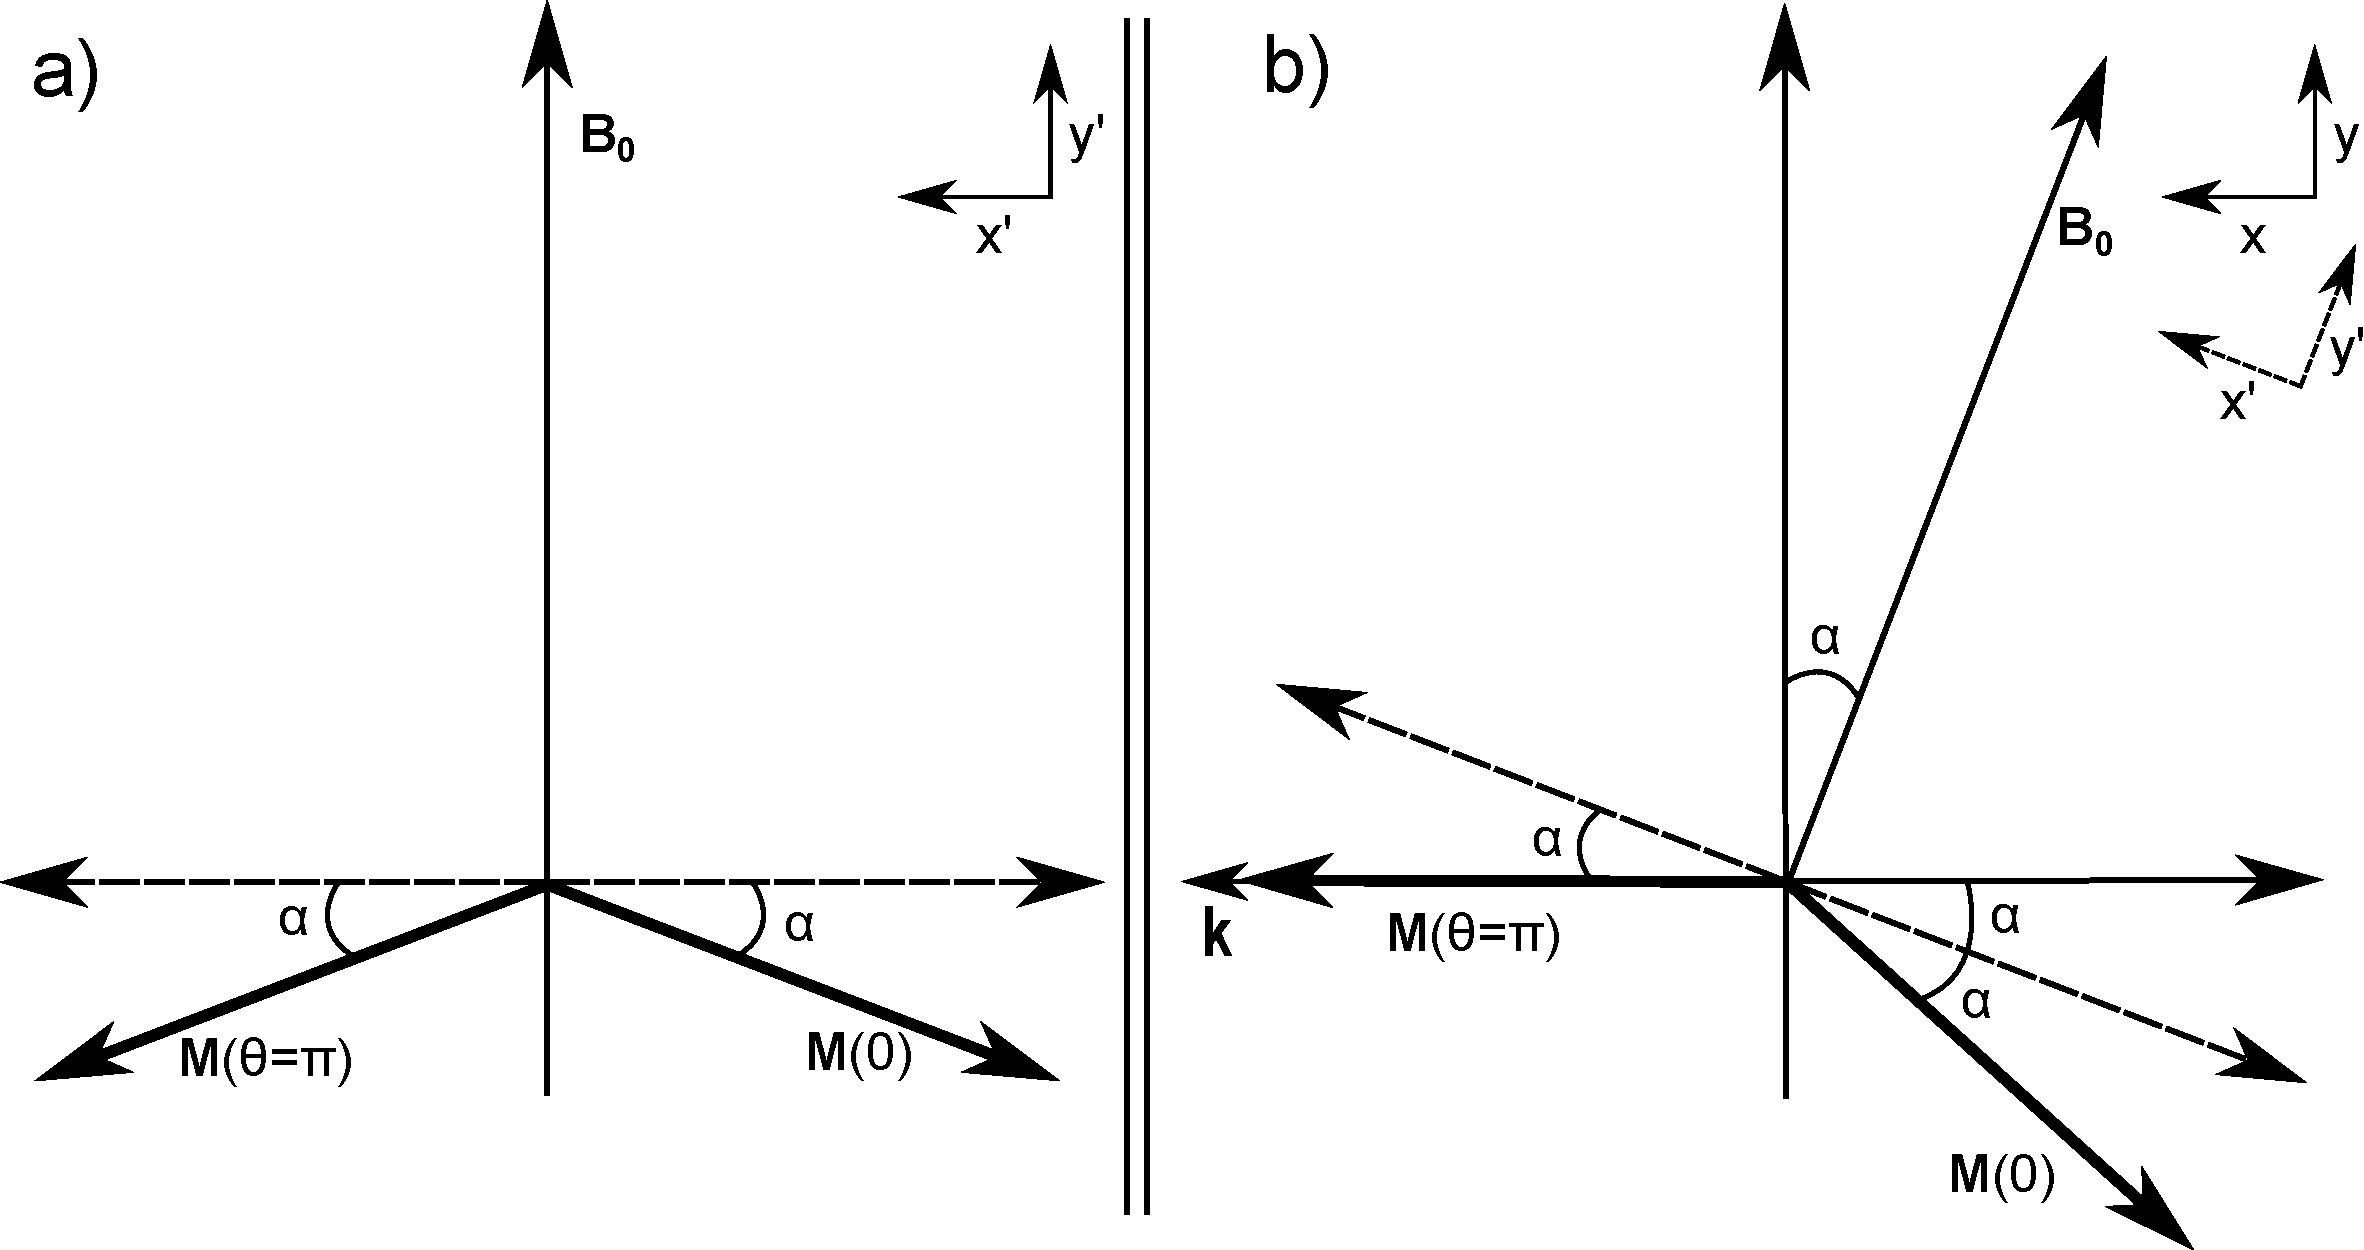
\includegraphics[scale=0.35]{Figures/Field_misalignment.pdf}
\end{center}
\caption[Precession with mis-aligned fields]%
{\narrower A diagram of the precessing magnetization vector $\mathbf{M}(t)$ with a non-zero projection onto the magnetic field $\mathbf{B}_0.$ a) A simplified diagram with $\mathbf{B}_0$ directed onto the $\hat{y}$ axis and $\mathbf{M}(t)$ making a constant angle $\alpha$ with the $\hat{x}-\hat{z}$ plane. b) The transformed diagram showing the vector arrangement from (a) rotated by $\alpha$ so that the atoms are polarized horizontally along the light propagation vector $\mathbf{k}$, with $\mathbf{B}_0$ misalinged by an angle $\alpha$ from the vertical direction $\hat{y}$. In both cases the simple harmonic form of the signal $\mathbf{M}(t) \cdot \mathbf{k}$ is preserved, with a reduction in amplitude from the case with $\alpha = 0$ and a small offset from 0 in case (b).}
\label{FieldMisalign}
\end{figure}
Given that the atoms are assumed above to be polarized perpendicular to $\mathbf{B}_0,$ it may appear that the signal will become distorted if the $\mathbf{k}$ vector and the initial magnetization $\mathbf{M}(t=0)$ at the end of the pump period are not orthogonal to the magnetic field axis. Consideration of the states on the Bloch sphere shows that an ensemble of atoms polarized at a non-zero angle $\beta$ relative to a constant applied field $\mathbf{B}_0$ will precess at the Larmor frequency independently of the value of $\beta$, which will also remain constant \cite[7.3]{Foot}. This arrangement is illustrated in Figure \ref{FieldMisalign} (a), where $\mathbf{B}_0$ is defined to be vertical, but the magnetization makes some constant angle $\alpha = \beta-\pi/2$ with the horizontal plane. In the primed coordinate system, we have
\begin{equation}
\mathbf{M}(\theta) = M_0(\hat{x'}\cos\alpha\cos\theta + \hat{z'}\cos\alpha\sin\theta  - \hat{y'}\sin\alpha). 
\end{equation}
With $\mathbf{k}$ aligned with the $\hat{x'}$-axis, the signal then becomes
\begin{equation}
\zeta(t) = A\cos\alpha\cos(\omega t + \phi) e^{-t/\tau}.
\end{equation}

From the diagram (a), we can move to a realistic depiction of a tilted field by changing to a rotated coordinate system such that $\hat{x} = \hat{x'}\cos\alpha - \hat{y'}\sin\alpha$ and $\hat{y} = \hat{y'}\cos\alpha + \hat{x'}\sin\alpha,$ as shown in Figure \ref{FieldMisalign} (b). In this picture, the field $\mathbf{B}_0$ is at an angle $\alpha$ to the vertical ($\hat{y}$) axis, and the initial atomic polarization is horizontal in line with the $\mathbf{k}$ vector. Then taking the projection of $\mathbf{M}(\theta)$ onto the $\hat{x}$-axis, it can be shown that the precession signal takes the form
\begin{equation}
\zeta(t) = A[\sin^2\alpha - \cos^2\alpha\cos(\omega t + \phi)] e^{-t/\tau}
\end{equation}
which (for constant $\alpha$) is equivalent to the original signal with amplitude reduced by a factor of $\cos^2\alpha$ and an offset equal to $A\sin^2\alpha.$

\section{DC Stark effect}
Application of an external static electric field can perturb the energy levels in both the initial and final states of an atomic transition. For a given state of total angular momentum $\mathbf{F} = \mathbf{I} +\mathbf{J}$ and a magnetic sublevel $m_F$, the quadratic Stark shift $W(F,m_F)$ is given by
\begin{equation}
W(F,m_F) = -\frac{1}{2}\alpha_0 E^2 - \alpha_2 \dfrac{[3m^2_F-F(F+1)][3X(X-1)-4F(F+1)J(J+1)](3E_Z^2-E^2)}{(2F+3)(2F+2)2F(2F-1)2J(2J-1)}
\end{equation}
where $\alpha_0$ is the scalar polarizability, $\alpha_2$ is the tensor polarizability, $X=F(F+1)+J(J+1)-I(I+1)$, and $E_z$ is the projection of the electric field onto the quantization axis \cite{Stark_Shift_expression}. The tensor polarization term is proportional to $[3m^2_F-F(F+1)],$ which evaluates to zero for both magnetic sublevels of a state with $F=1/2$. Thus, the ground state sublevels and the $F=1/2$ part of the excited state manifold in $^{199}$Hg acquire common shifts in an electric field and cannot contribute to a systematic error. The value of the shift for the $6^1S_0 \rightarrow 6 ^3P_1$ transition in $^{199}$Hg was measured in \cite{2000_Hg_Stark_Shift}, resulting in a value of $23.326 \pm 0.06$ kHz/(kV/cm$^2$). The quadratic Stark shift is independent of the electric field direction and also common to the two ground state hyperfine sublevels, so it cannot induce a false EDM signal. However, it provides a handle on any effect which may couple to the magnitude of the electric field (which may be different for opposite polarities), and was regularly monitored during the course of EDM data taking. The results of the Stark shift measurements are given in Section \ref{|E|_effects} in the context of systematic errors.

\section{Scalar and vector light shifts}
The presence of light on or near resonance with an atomic transition can cause shifts in the relevant energy levels. These shifts can be broken into components which are independent of the atomic spin direction (scalar light shifts) and which depend on the atomic spin direction (vector light shifts) \cite{Swallows, 1967_Optical_pumping_light_shifts}. Of the two, only the latter can lead to a differential shift in the ground state hyperfine sublevels which can mimic an EDM. This vector light shift acts as an effective magnetic field oriented along $\mathbf{k}$, with a magnitude proportional to the degree of circular polarization. Therefore, the induced energy shift during the probe phase is nonzero only if the probe light has some non-zero residual circular polarization, and it also averages to zero unless the atomic polarization does not remain coplanar with $\mathbf{k}$ during and after the pump phase. \cite{Swallows} explains how the magnetization may acquire a non-zero projection in the plane orthogonal to $\mathbf{k}$ due to the circular polarization and increased intensity of the pump beam, coupled to a mismatch in the  frequency of precession and the pump light chopping frequency. The effect of vector light shifts on the latest EDM dataset is illustrated in Figure \ref{TDiffVsPhaseFit} and discussed in Section \ref{light_shift_noise}. While probe-phase light shifts due to vertical magnetization are observable, they should be independent of the electric field direction. As such, the shifts do not contribute to a potential systematic error unless the probe light polarization or propagation vector $\mathbf{k}$ is coupled to the applied electric field \cite{Griffith}. 

\section{Stark interference}
A false EDM signal would present itself as a relative shift in the Zeeman sublevels of the ground state or the $F=1/2$ excited states which scales linearly with the applied electric field. Neither the vector light shift nor the quadratic Stark effect can generate such a false signal, but an external $\mathbf{E}$ can induce mixing between the electric quadrupole (E2) and magnetic dipole (M1) couplings to the $F=1/2 \rightarrow F=1/2$ transition in such a way that it causes a shift in the absorption profile of the Hg vapor. The fractional change in the absorptivity $\alpha$ is given by \cite{Griffith}
\begin{equation}
\delta\alpha/\alpha = (a_{E2}+a_{M1})(\hat{\mathbf{\epsilon}}\cdot\mathbf{E})(\hat{\mathbf{k}}\times\hat{\mathbf{\epsilon}})\cdot\mathbf{\sigma}
\end{equation}
where $\hat{\mathbf{\epsilon}}$ is the light polarization vector, $\mathbf{\sigma}$ is the nuclear spin polarization, and $a_{E2}$ and $a_{M1}$ are the electric quadrupole and magnetic dipole mixing amplitudes, respectively. The vector character causes the shift to vanish if the light is linearly polarized either parallel or perpendicular to $\mathbf{E}$. The light used to probe the atoms in the EDM experiment is vertically polarized, so the projection of $\mathbf{\hat{\epsilon}}$ onto $\mathbf{E}$ is maximal, and any potential Stark interference acts as an effective magnetic field in the direction of $(\hat{\mathbf{k}}\times\hat{\mathbf{\epsilon}})$. If the polarization is not exactly parallel to $\mathbf{E}$, this effective field has a non-zero projection onto $\mathbf{B_0}$, which can lead to an EDM-like frequency shift coupled to the direction and magnitude of $\mathbf{E}$. The size of this effect was measured in \cite{2011_Hg_Stark_Interference} using probe light polarized at $\pm45^{\circ}$ to the electric field; the value obtained for the combined M1 + E2 interference amplitude is
\begin{equation}
a_{M1}+a_{E2} = (5.8 \pm 1.5) \cdot 10^{-9} \text{(kV/cm)}^{-1}.
\end{equation}
While the potential for frequency shifts due to light shifts (and HV-coupled beam deflection) or Stark interference was a cause for concern in previous iterations of the experiment, the new method of data taking involves blocking the probe beam entirely during the measurement time and is therefore insensitive to the class of systematics induced by the probe light.

\chapter{Methodology}
This chapter details the construction of the mercury EDM experimental apparatus, including the optical systems used to generate resonant 254 nm laser light, the magnetic field coil and associated magnetic shielding, and the electrical systems used to apply the high voltage to the cells and measure the resulting current flow.
The mercury vapor cells are not included, as they are of such importance to warrant a separate chapter.
\section{Optical setup}
\subsection{UV laser light generation}
The UV laser light used to pump and probe the atoms is generated using a commercially-available frequency-quadrupled infrared (IR) diode laser system purchased from Toptica photonics AG to replace a similar 'home-built' system used in previous iterations of this experiment \cite{2001_Hg_EDM, 2009_Hg_EDM}. Infrared light from a high-power, grating-stabilized laser diode operating at 1016nm passes through two traveling-wave resonant cavities with birefringent crystals placed at one of the beam waists inside. The first (IR to green) cavity uses a potassium niobate (KNbO$_3$) crystal, while the second (green to UV) cavity uses beta barium borate (BBO). With 140 mW of input IR diode laser power, the system typically outputs 40mW of green light and 100 $\mu$W of UV, dependent on cavity fine tuning and the quality of each cavity's input beam coupling. 

\subsection{Optical harmonic generation}
The UV laser system in use in the Hg EDM experiment exploits a scheme based on nonlinear optics known as second harmonic generation (SHG) in order to obtain ultraviolet light from an infrared laser diode. For the case of a general dielectric material in the presence of a driving radiation field $\mathbf{E}$, we can describe the response of the material by relating the components of the polarization field $\mathbf{P}$ to the displacement field $\mathbf{D}$ and the electric susceptibility tensor $\chi_{ij}$: 
\begin{equation} D_i = \epsilon_0 (1+\chi_{ij})E_j = \epsilon_0E_i + P_i.\end{equation} For the case of an isotropic material, the susceptibility tensor reduces to $\chi_{ij} = \delta_{ij} \chi_0$, and the polarization field is directly proportional to $\mathbf{E}$: 
\begin{equation} P_i = \epsilon_0\chi_0E_i. \end{equation} 
In general, the susceptibility tensor may take on different values along various axes according to the properties of the material involved.
	
If we allow for the possibility of non-linear polarization terms proportional to $\mathbf{E}^2$, $\mathbf{E}^3$, and so on, we can write 
\begin{equation} \mathbf{P} = \epsilon_0\chi_{ij}\mathbf{E} (1 + \dfrac{E^2}{E_2^2} + \dfrac{E^3}{E_3^2} ...) \end{equation} where $(E_2,E_3...)$ are field values that describe the non-linear electrical properties of the medium. In general, these non-linear electric field strengths will be comparable to the fields inside the dielectric medium and will be much larger than the applied field $E$ \cite{1961_Franken_SHG}. If the driving field has harmonic time dependence $E_i cos (\omega t)$, then to second-order the response of the polarization field will be 
\begin{equation} P_i = \epsilon_0\chi_{ij} (E_j cos(\omega t) + \dfrac{E_j^2}{E_2^2} cos^2(\omega t)+...). \end{equation}
Noting that $cos^2(\omega t) = (1/2)[cos(2\omega t)+1]$, we find 
\begin{equation} P_i = \epsilon_0\chi_{ij} (E_j cos(\omega t) + \dfrac{E_j^2}{2E_2^2}[1+cos(2\omega t)]).\end{equation}

The polarization field has now taken on a component that oscillates at twice the frequency of the driving field, which will produce output light at exactly half of the input wavelength. The first experimental realization of higher harmonic generation with visible light was reported by Franken \textit{et. al.} in 1961, using a high-power 694.3 nm ruby laser making a single pass through a crystalline sample of quartz \cite{1961_Franken_SHG}. Note that the amplitude of the second harmonic in the above equation is proportional to the square of the amplitude of the driving radiation field $\mathbf{E}$. Because of this nonlinearity, present-day implementations of SHG involve crystals placed inside of resonant optical cavities, where the stored power may be many thousands of times higher than that of the input beam, with a corresponding increase in harmonic conversion efficiency.\footnote{It is also amusing to note that in the original paper detailing the discovery of SHG, the photographic evidence of a second-harmonic beam was erased by an editor who mistook the frequency-doubled beam spot for a speck of dust on the exposed plate.}  

\subsection{Frequency doubling cavities}
The nonlinear crystal employed in the 1016 $\rightarrow$ 508 nm cavity is potassium niobate (KNbO$_3$), while the 508 $\rightarrow$ 254 nm cavity uses beta-barium borate (also referred to as BBO), which has a smaller nonlinear response than KNbO$_3$ but is necessary for its UV-transparent properties. Both are negative uniaxial crystals, meaning that two of the three principal axes feature equal indexes of refraction (defined to be the ordinary index $n_o$), while the extraordinary index of refraction $n_e < n_o$ for waves polarized along the \textit{optic axis} \cite{New}.\footnote{While materials with a unique optic axis are referred to as uniaxial, those with three distinct indexes of refraction are nonetheless said to possess only two optic axes and are therefore labeled `biaxial'.}

The frequency doubling cavities in the UV laser system are constructed in a traveling-wave, ``bow-tie'' configuration detailed extensively in \cite{Nagourney}. Each cavity consists of two planar mirrors situated on either end of the long arm of the bow tie, and two curved mirrors on either end of the shorter arm. In this configuration, the cavity has two beam waists, the smaller of which is in the center of the short arm. The nonlinear crystal is placed at this beam waist because the harmonic generation efficiency is proportional to the optical power density inside the crystal, and the smallest beam waist maximizes the power density.

\begin{figure}
\begin{center}
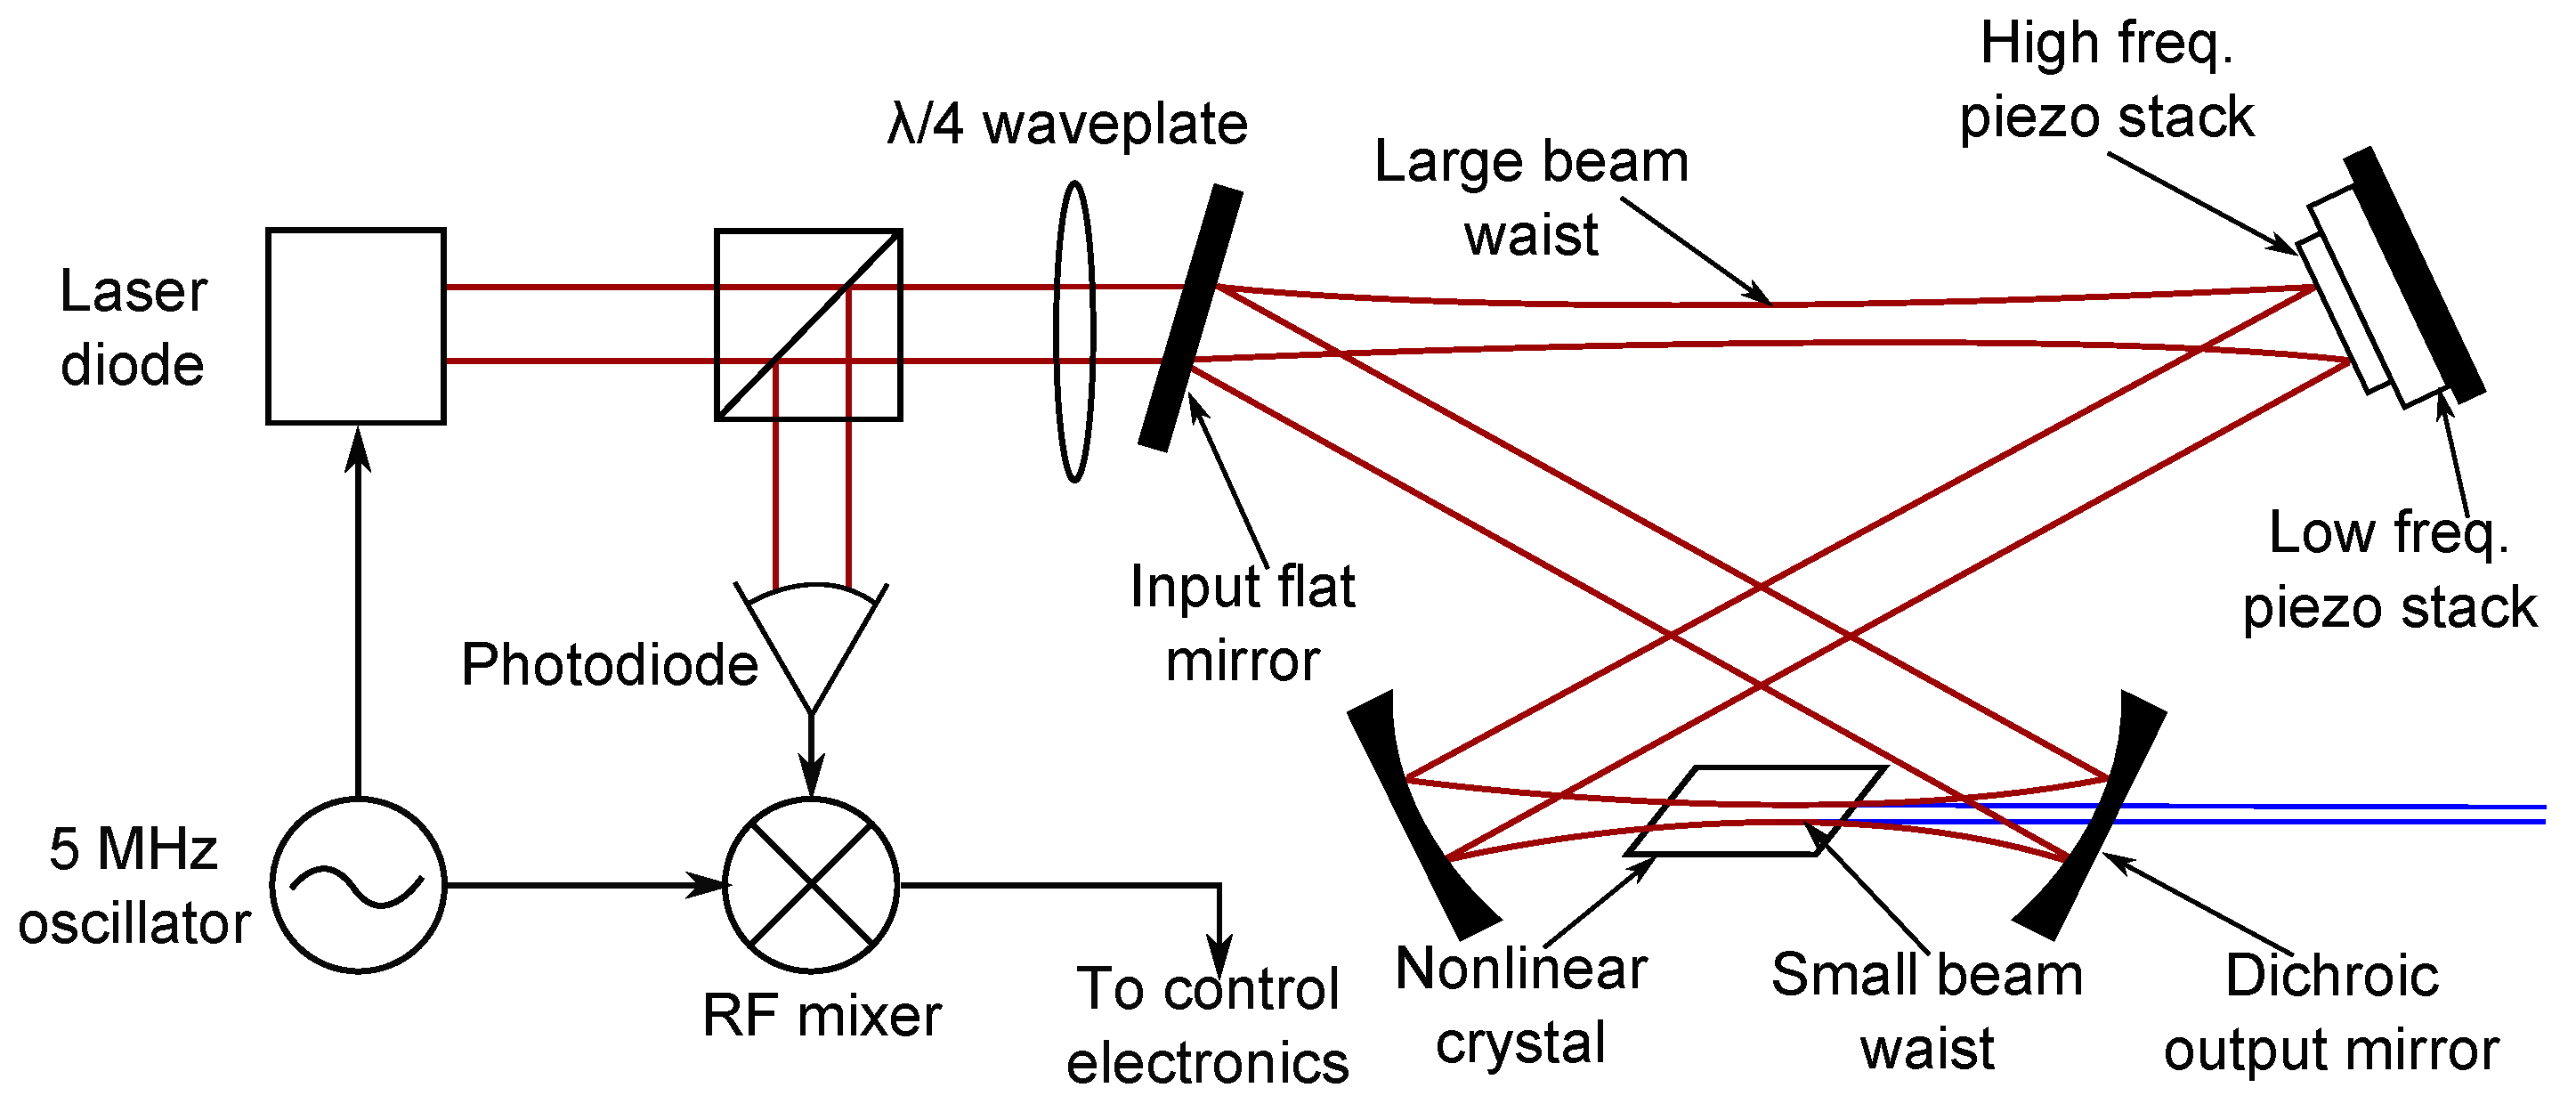
\includegraphics[scale=0.3]{Figures/SHG_Cavity_Diagram.pdf}
\end{center}
\caption[Second harmonic generation cavity]
{\narrower A diagram of the system used to generate frequency-doubled laser beams. The laser system used in this work (Toptica 254 nm FHG pro) utilizes the PDH locking scheme to keep the cavity length on resonance. A 5 MHz signal is applied to the laser diode current, and the resulting amplitude modulation from the near-resonant cavity is used to generate an error signal. A compound piezo stack is used in each of the two cavities for separate high-frequency and low-frequency feedback. The feedback loop connects the voltages across the piezos to the error signal generated by the RF mixer output.}
\label{CavityDiagram}
\end{figure}

\subsection{Feedback control systems}
The frequency-doubling cavities inside the laser system use piezo-mounted mirrors to maintain the cavity at a total length that matches an integer number of wavelengths of the input beam. In the laser system currently in use, the Pound-Drever-Hall method is used to stabilize each cavity on resonance with the input light.\footnote{The PDH method was initially developed to stabilize a laser wavelength to a cavity resonance, but it can just as easily be used to hold a cavity on resonance with an un-stabilized laser.} In this setup, the laser is phase modulated by applying a 5 MHz oscillating signal $\omega_m$ to the laser diode current. The modulation introduces sidebands in the frequency domain at $\omega_0 + \omega_m$ and $\omega_0 - \omega_m$. If the modulation frequency is larger than the cavity linewidth, the various frequency components of the phase-modulated beam will be selectively absorbed by the cavity when the central frequency is near a resonance. The action of the cavity induces amplitude modulation in a phase-modulated beam.

The error signal is derived from the frequency spectrum of the rejected beam from from the cavity. The beam exiting the cavity from the input mirror passes through a $\lambda/4$ waveplate and polarizing beam splitter to deflect it onto a photodetector. The detector signal is then input to an RF mixer along with the modulation signal, which detects the portion of the input intensity signal at $\omega_m$. Away from resonance, one of the sidebands will be closer to the resonant frequency of the cavity than the other, and the relative phase between the amplitude-modulated signal and the modulation signal will change sign as the cavity length is swept across the resonance condition \cite{Nagourney}. 

\subsection{Phase matching}
Beyond the need to maintain high-power density for efficient SHG, the frequency dependence of the index of refraction $n(\omega)$ in bulk matter creates a second difficulty: if the fundamental wave and the second harmonic do not remain in-phase as they propagate through the crystal, there is no coherent build-up in harmonic intensity. Because the index of refraction determines the relationship between frequency and wavelength, it becomes necessary to tune the refractive index of the crystal for the second harmonic to match that of the input beam. In practice this is achieved through \textit{angle-tuned phase matching}, which exploits the angular dependence of the refractive index of the extraordinary wave $\tilde{n}_e(\omega,\theta)$, a quantity which varies between $n_o$ and $n_e$ according to
\begin{equation}
\dfrac{1}{\tilde{n}_e(\theta)} = \sqrt{\dfrac{\cos^2(\theta)}{n_o^2} + \dfrac{\sin^2(\theta)}{n_e^2}}
\end{equation}
where $\theta$ is the angle between the propagation vector $\mathbf{k}$ and the optic axis \cite{New}. By playing this angular dependence for the extraordinary wave against the frequency dependence of $n_o(\omega)$ for the ordinary wave, an angle $\theta$ can be found to satisfy
$\tilde{n}_e(2\omega,\theta) = n_o(\omega)$ for a given input light frequency $\omega$.\footnote{For a uniaxial crystal, there is no angular dependence for the ordinary refractive index $n_o$.} In both cavities the crystal is tuned to match the ordinary index $n_o$ for the fundamental frequency to $\tilde{n}_e$ for the second harmonic, so the input light must have ordinary polarization while the frequency-doubled beam has the extraordinary polarization, a scheme known as \textit{Type I ooe phase matching} \cite{Swallows}. 

\begin{figure}
\begin{center}
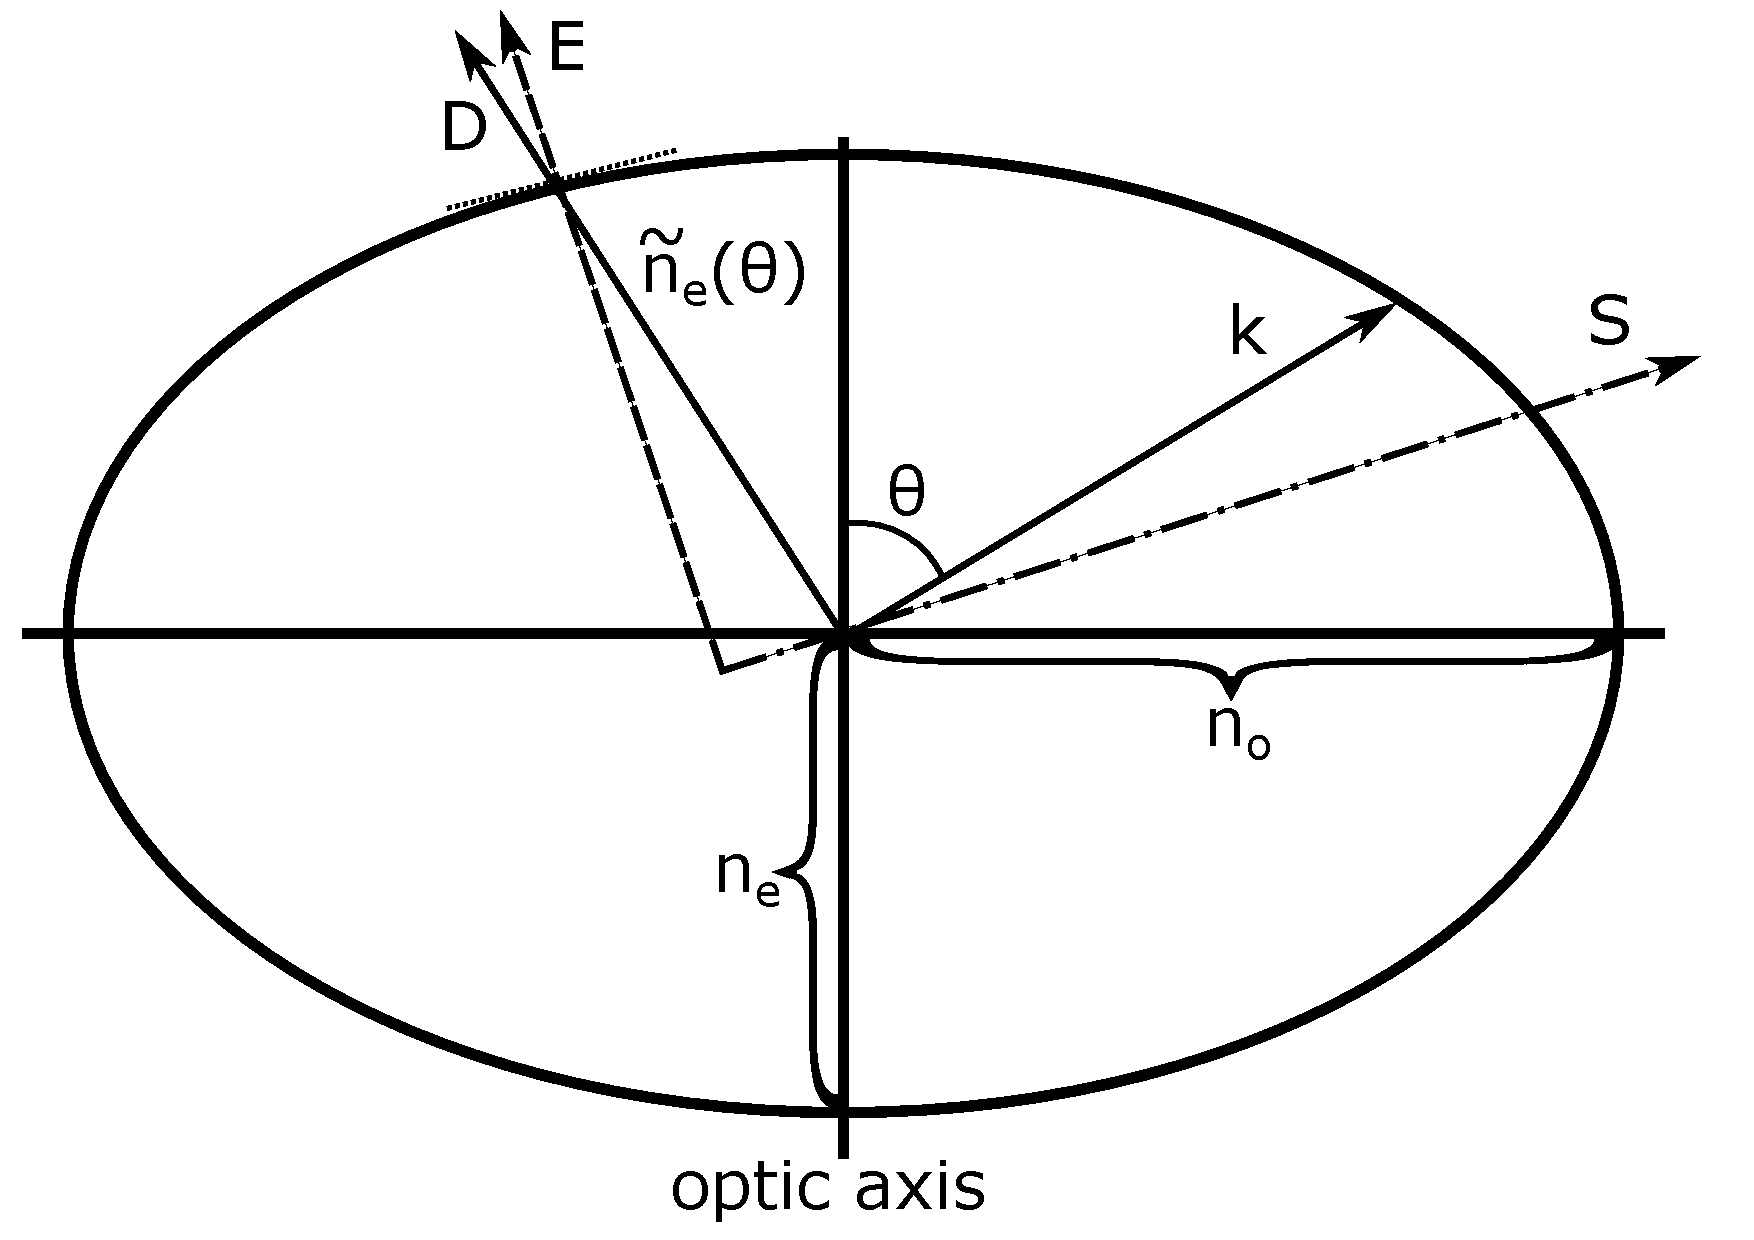
\includegraphics[scale=0.3]{Figures/refractive_index.pdf}
\end{center}
\caption[Refractive index ellipsoid section in negative uniaxial medium]
{\narrower The index of refraction for a wave polarized in the plane of the page propagating at an angle $\theta$ to the optic axis. The distance along the vector $\mathbf{D}$ from the origin to the surface of the ellipse corresponds to the index of refraction for a wave with extraordinary polarization $\tilde{n}_e$, which may vary from $n_o$ (for waves propagating along the optic axis) to $n_e$. Ordinary waves (polarized orthogonal to the plane of the page) have an index of refraction $n_o$ regardless of the direction of phase propagation $\mathbf{k}$. While $\mathbf{D}$ is always orthogonal to $\mathbf{k}$, $\mathbf{E}$ is normal to the ellipse, so the Poynting vector $\mathbf{S}$ is not generally parallel to $\mathbf{k}$, leading to `walk off' effects. Adapted from \cite{New}, Figure 3.4.}
\label{IndexDiagram}
\end{figure}

\subsection{Laser wavelength locking}
The laser wavelength is stabilized to the $F = 1/2 \rightarrow F = 1/2$ transition in $^{199}$Hg by applying a voltage offset to the a piezoelectric crystal mounted to a reflection grating inside the laser diode cavity. The voltage is derived by comparing the intensity of the laser beam picked off from the front face of a wedged quartz crystal to the intensity transmitted through a ``reference cell'' filled with natural (isotopically mixed) Hg, measured using the light picked off from the back face of the quartz wedge. The two intensity signals are generated from photodiodes and passed to an analog electronic circuit that compares the ratio to a set point and generates a corresponding error signal which is sent to a high voltage amplifier and then applied to the piezo stack on the retroreflective grating in the IR diode cavity. 

\subsection{Optical chopper} 
During the pump period, the weak laser light intensity requires a time much greater than a single precession period to polarize most of the atoms in the cell. Because $\mathbf{B}_0$ is perpendicular to the light propagation axis (and the atomic polarization), the light must be modulated at the average Larmor frequency of the four cells to prevent the atoms from depolarizing as they begin to precess. The modulation is performed using a New Focus model 3501 chopper wheel, driven by a TTL square wave output from an SRS DS345 function generator. While the 3501 features an integrated optical feedback system connected directly to the chopper wheel, the extremely low atomic precession frequency will introduce substantial time jitter if the feedback loop is to follow the wheel directly. At the minimum frequency of 4 Hz, the spec-sheet time jitter is listed as 0.5 ms peak-to-peak. Near 5 kHz, the time jitter is reduced to 2 $\mu$s peak-to-peak. To obviate the time jitter problem, the chopper wheel is driven by a DC brush motor connected to an HP model HEDS-5540 optical encoder which increases the frequency of the TTL input signal by a factor of 250. The chopper wheel itself has two cut out wedges which enables the duty cycle of the pump light to be set; we use an opening angle of 48$^{\circ}$, for a duty cycle of 26.7\%.

\section{Cell vessel construction}
The walls of the vessel were made using 1/2'' thick graphite-impregnated ultra-high molecular weight polyethylene (UHMW-PE), marketed under the trade name Tivar\textregistered 1000 anti-static. Measured values for the surface resistivity of the Tivar ranged from 70-100 k$\Omega$/square.\footnote{Surface resistivity has units of $\Omega$/square because the measured resistance between two linear electrodes on the surface is inversely proportional to the electrode length and directly proportional to the distance in between. Only the ratio of distances enters the conversion from resistance to resistivity, so the latter takes on units of $\Omega$/square.}
The interior of the vessel is 5'' in length, and the interior cross section (orthogonal to the shield axis) is 4'' square. The top and bottom vessel walls include a recessed circular area with a chamfer near the outer rim of the HV electrodes to maintain the 10 mm distance to ground on the outer electrode surfaces.
\begin{figure}
\begin{center}
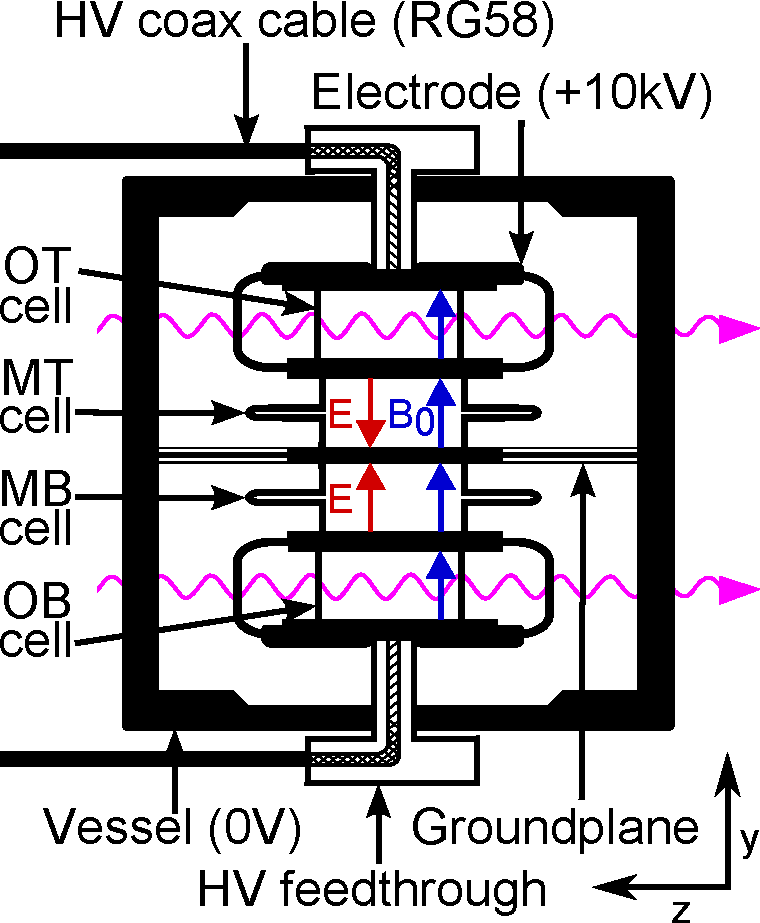
\includegraphics[scale=0.6]{Figures/Vessel_Diagram.pdf}
\end{center}
\caption[Section of EDM vessel]{\narrower Cross-sectional diagram of the EDM cell vessel (not to scale) showing the high voltage (HV) cables, groundplane, and a cut-away view of the HV electrodes and feedthroughs. The laser beams through the outer cells traverse the apparatus along the shield axis (z-axis), while the middle cell beams travel along the x-axis.}
\label{Vessel_Diagram}
\end{figure}

The vessel is divided in half by a groundplane made from 3 sandwiched layers of 1/16'' fused silica, bonded with UV-curing epoxy. The top and bottom plates have circular holes to accept the MT and MB cell endcaps, similar to the 1/16'' recesses in the HV electrode surfaces. When properly seated, the cell endcaps sit flush with the groundplane and the inner electrode surfaces to maintain the 10 mm distance between high-field surfaces. In addition to minimizing  the possibility for electrical breakdown, these recesses also locate the cells relative to each other and constrain any motion of the cell stack.

The HV electrodes are made from Tivar and are assembled around the outer cells using four nylon bolts, which hold down the smaller piece of the electrode when screwed into the main body. The electrode 'lids' are recessed to accept the HV feedthroughs which hold each electrode in place; at the bottom of each electrode recess is a SnO$_2$-coated disk which is glued to the Tivar using conducting silver epoxy. The silver epoxy is applied in three separate drops around the rim of the disk, to prevent a circular path for eddy currents which could influence the precession frequencies of the outer cells. 

\section{Magnetic field generation and shielding}
\subsection{Magnet coil}	
\begin{figure}[ht]
\begin{center}
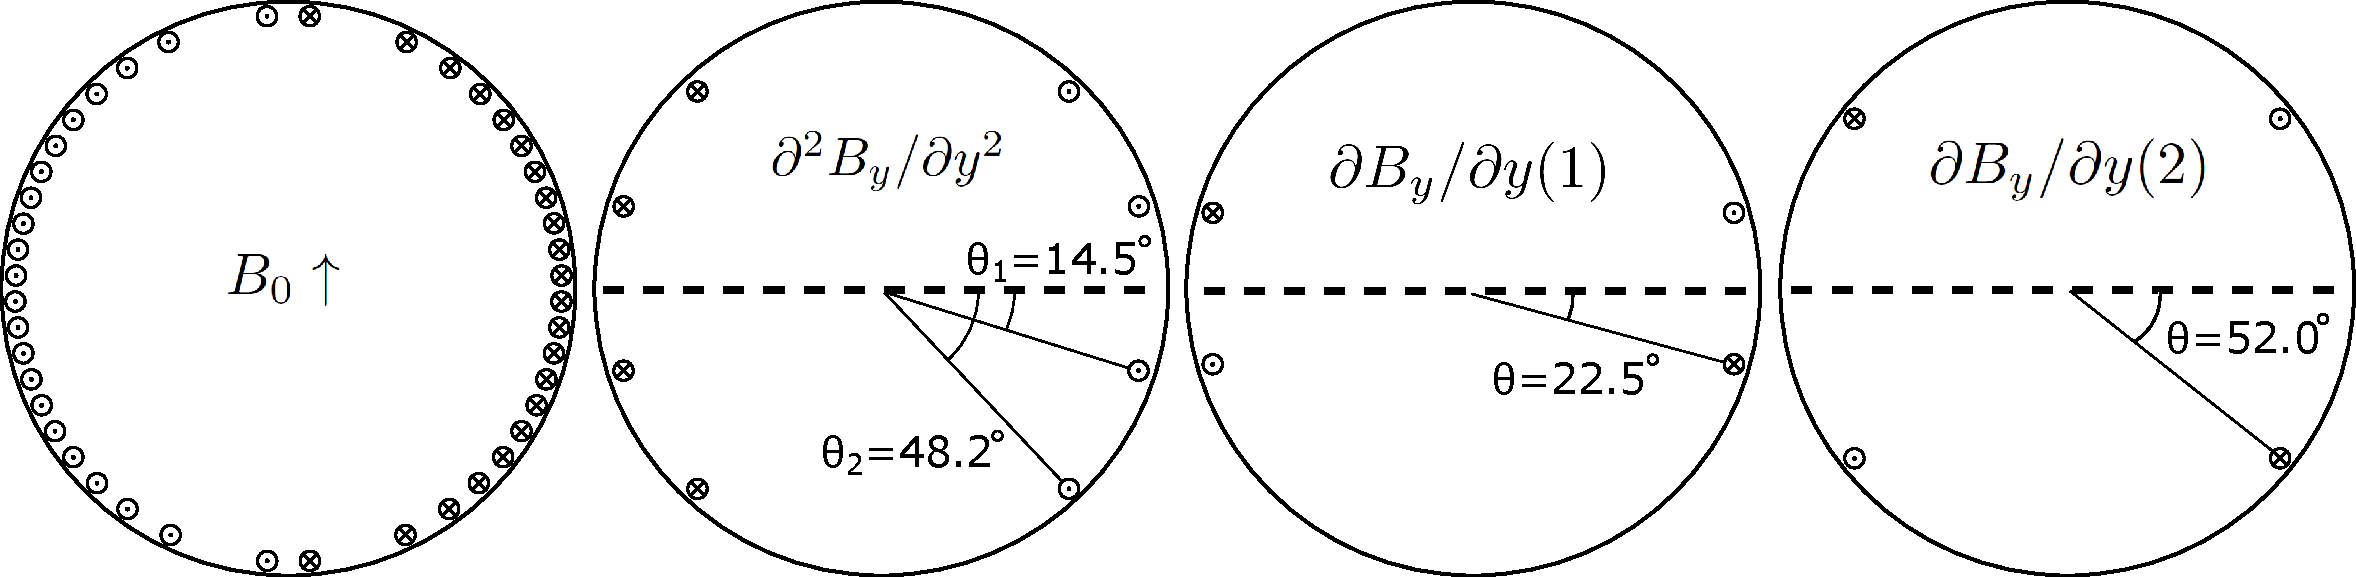
\includegraphics[scale=0.37]{Figures/Coil_Current_Dist_On_Axis.pdf}
\end{center}
\caption[$\cos(\theta)$ coil and vertical gradient coil current pattern]
{\narrower A schematic cross section of the distribution of current paths down the axis of the main coil form and magnetic shields. The primary $\cos(\theta)$ magnet coil has 30 windings, some of which have been omitted from the diagram for detail. The second-order gradient coil is also a $\cos(\theta)$ coil with only 4 windings, which creates a magnetic field (and a second-order gradient) in the direction opposite $\mathbf{B}_0$. The first-order gradient coils $\partial B_y/\partial y (1)$ and $(2)$ both have have 2 windings, with current in the opposite directions so neither gradient coil contributes to the average field.}
\label{Coil_Currents_On_Axis}
\end{figure}

To take advantage of the cylindrical magnetic shield geometry, the bias magnetic field $\mathbf{B}_0$ is orthogonal to the shield axis. For a cylindrical shield with finite length greater than its radius, the set of windings which produces a maximally-uniform field in the radial direction is a series of rectangular loops with long edges set at constant radius and distributed equidistantly in the vertical direction. For a given coil radius this arrangement corresponds to constant intervals of $\cos(\theta)$, and this type of coil is typically referred to as a $\cos(\theta)$-coil \cite{Griffith}. The primary magnet coil used in this work has 30 windings which are situated on the outer surface of a cylindrical form made of linen-based phenolic laminate (grade LE), purchased as a tube from Boedecker Plastics.\footnote{The coil form used in previous iterations of this experiment was made of aluminum, which could contribute substantial magnetic noise at our current level of sensitivity (assuming it remains the closest conductor to the Hg atoms) due to thermal motion of charge carriers at finite temperature \cite{Swallows}.}

\begin{figure}[ht]
\begin{center}
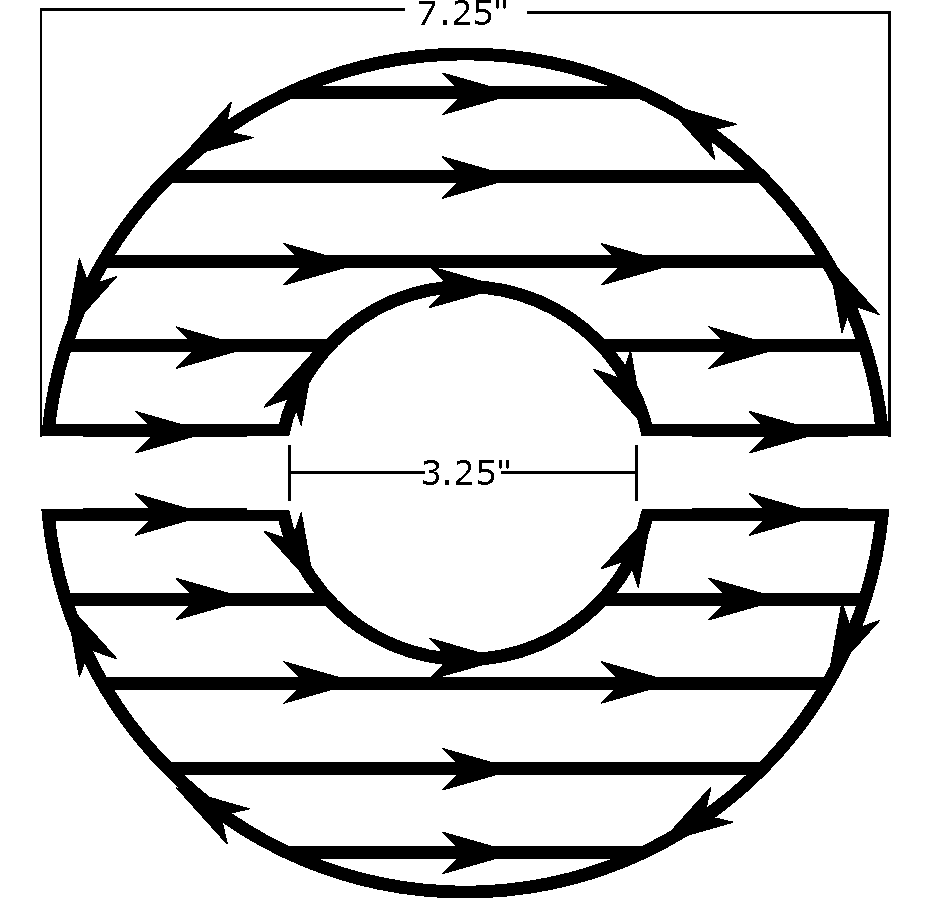
\includegraphics[scale=0.4]{Figures/EndcapCoilCurrent.pdf}
\end{center}
\caption[Endcap coil current pattern]
{\narrower A diagram of the path taken by currents in the endcap coils on either end of the $\cos(\theta)$ coil which produces $\mathbf{B}_0$. Solid lines indicate the paths of the windings across the face and around the inner and outer rim; arrows indicate the direction of current flow. The outer rim windings are set up to cancel the current density around either rim of the cylindrical coil form, together approximating the ideal distribution of rectangular loops.}
\label{Endcap_Coil_Current}
\end{figure}

Because the ends of the magnet coil must remain open to facilitate installation and removal of the vessel, the windings on the cylindrical form are not complete rectangles. Instead, each winding runs parallel to the axis of the cylinder from end to end and loops around the outer rim in a semicircle at each end to return down the other side. To improve the uniformity of the field, several sets of removable ``endcap coils'' were made to fit just inside the lip on either end of the main coil form. The endcap coils are wound on two circular forms of the same laminate the cylindrical coil form is made of, and the current distribution consists of a set of parallel lines spaced equally in the vertical direction, with semi-circular return loops. The direction of the current in the endcap coils is chosen so that the semi-circular windings on the endcaps cancel the current density of the corresponding windings on the cylindrical form. Although there are only 10 sets of windings on each endcap coil, this setup more closely approximates the ideal set of equally-spaced complete rectangular loops for a more uniform field.

In addition to the primary coil and endcap coils, several gradient coils were wound on the cylindrical form  to correct the gradients produced by the main coil. Two sets of linear gradient coils ($\partial B_y/\partial y(1)$ and $\partial B_y/\partial y(2)$) were wound in the same manner as the primary coil with long edges parallel to the coil form axis, but each coil has only one pair of windings arranged symmetrically about the vertical center of the coil form, with current going in the opposite sense between the two. The linear gradient coils therefore produce no net magnetic flux and little or no change to the average field. The second-order gradient coil is a $\cos(\theta)$ coil with fewer windings than the primary coil, which creates a non-zero average field in the direction opposite $\mathbf{B}_0$. For this reason, the second-order coil is connected to the primary coil in series, to ensure that any current fluctuations are common-mode. The second-order gradient coil generates a larger $\partial^2 B_y/\partial y^2$ than the primary coil per unit of flux, oriented in the opposite direction to cancel the gradient of the primary coil over the volume occupied by the cells.

Several other sets of coils were wound on the coil form but are rarely used. These include a $\cos(\theta)$ coil oriented in the $x$-direction (orthogonal to $\mathbf{B}_0$) with 26 windings, a 17'' solenoid with turns every $1/4$'' to provide a uniform field $B_z$, first-order $\partial B_z/\partial z$ ($\pm 2.0$'' from the center line) and second-order $\partial^2 B_z/\partial z^2$ ($\pm 6.0$'', $5.5$'', and $5.0$'') gradient solenoids, and first-order $\partial B_y/\partial x$ and second-order $\partial^2 B_y/\partial x^2$, arranged as in Figure \ref{dBy-dx_Coils}.

\begin{figure}[ht]
\begin{center}
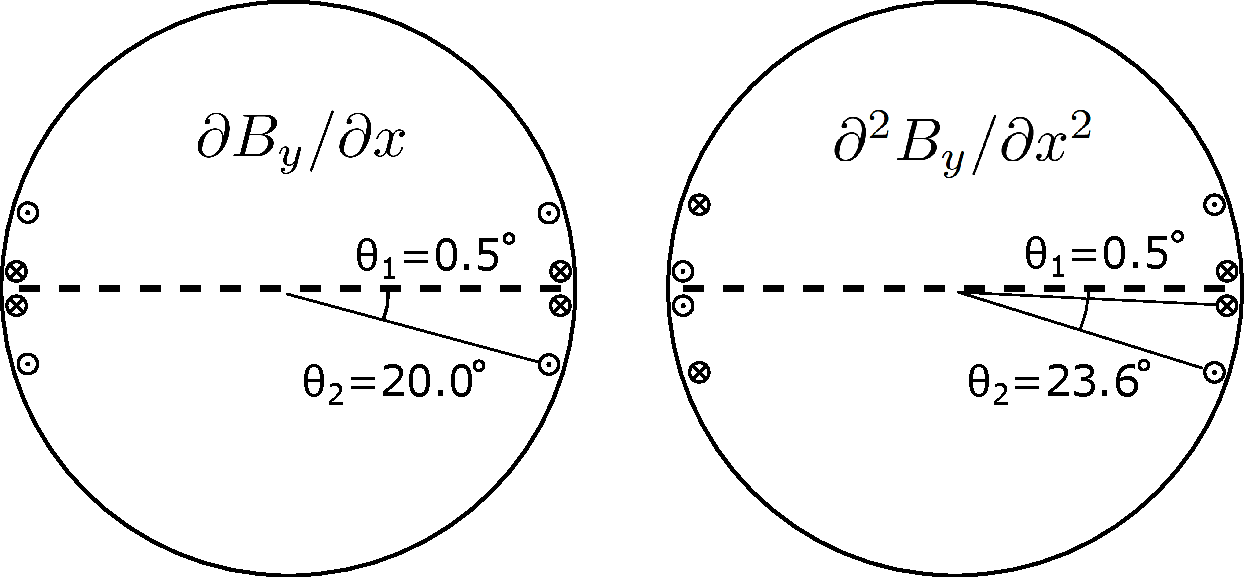
\includegraphics[scale=0.37]{Figures/dBy-dx_Coils.pdf}
\end{center}
\caption[Horizontal gradient coil current pattern]
{\narrower A cross section of the distribution of current paths to control gradients in the horizontal direction $\partial B_y/\partial x$ and $\partial^2 B_y/\partial x^2$.}
\label{dBy-dx_Coils}
\end{figure}

\begin{table}[ht]
\begin{center} 																							
\caption[Cell frequency dependence on magnet coil currents] 
{\narrower The frequency dependence of various cells and combinations on magnetic gradient coil currents. All values are specified in units of s$^{-1}$ per mA of current through the magnet coil.} \label{Grad_Coil_Current_vs_Freq}	
\begin{tabular}{cccc}
\hline \hline 
Frequency Channel & $\partial B_y/\partial y (1)$ & $\partial B_y/\partial y (2)$ & Endcap coils  \\ [0.5ex]	
\hline                   														
Middle Top (MT) Cell & $-2.349\cdot 10^{-2}$ & $-3.425\cdot 10^{-2}$ & $2.656\cdot 10^{-3}$ \\
Middle Bottom (MB) Cell &  $2.371\cdot 10^{-2}$ &  $3.426\cdot 10^{-2}$ & $2.588\cdot 10^{-3}$ \\ 
Outer Top (OT) Cell & $-6.810\cdot 10^{-2}$ & $-1.062\cdot 10^{-1}$ & $-2.481\cdot 10^{-3}$ \\
Outer Bottom (OB) Cell &  $6.789\cdot 10^{-2}$ &  $1.061\cdot 10^{-1}$ & $-2.764\cdot 10^{-3}$ \\ 		 
Middle Cell Difference: MT-MB & $-4.720\cdot 10^{-2}$ & $-6.851\cdot 10^{-2}$ & $6.8\cdot 10^{-5}$ \\
Outer Cell Difference: OT-OB & $-1.360\cdot 10^{-1}$ & $-2.123\cdot 10^{-1}$ & $2.83\cdot 10^{-4}$ \\
Leak Test: (OT-MT)+(OB-MB) & $-4.263\cdot 10^{-3}$ & $-2.172\cdot 10^{-4}$ & $-1.049\cdot 10^{-1}$ \\
$\Delta\omega_{EDM}$: (MT-MB)- $\frac{1}{3}$(OT-OB) & $-1.869\cdot 10^{-2}$ & $2.246\cdot 10^{-2}$ & $-2.581\cdot 10^{-4}$ \\  
[1ex]	
\hline
\end{tabular}
\end{center} 														
\end{table}

Calibration numbers for the gradient coils that were used in the experiment are given in Table \ref{Grad_Coil_Current_vs_Freq}. While the gradient coil currents can be tuned to equalize the precession frequencies in all four vapor cells to a few parts in $10^7$, the values of the magnetic field gradients inside the vessel vary slightly each time the shields are degaussed, and are not identical for opposite directions of the main magnet coil current. In general, the field gradients created by the main coil and the second-order gradient coil $\partial^2 B_y/\partial y^2$ are larger when $\mathbf{B}_0$ is directed up, as seen in Table \ref{Main_Coil_Current_vs_Freq}. 

\begin{table}[ht]
\begin{center} 																							
\caption[Cell frequency dependence on $B_0$ coil and  $\partial^2 B_y/\partial y^2$ ] 
{\narrower The frequency dependence of various cells and combinations on the current through the main magnet coil and the second-order gradient coil $\partial^2 B_y/\partial y^2$, connected in series. The frequency dependence of each individual cell is given relative to the average frequency $\bar{\omega} = 5.341$ s$^{-1}$/mA.} \label{Main_Coil_Current_vs_Freq} 		
\begin{tabular}{ccc}
\hline \hline 
Frequency Channel & $B_0 \uparrow$ & $B_0 \downarrow$ \\ [0.5ex]		
\hline                   														
Middle Top (MT) Cell & $\bar{\omega} + 9.728\cdot 10^{-5}$ & $\bar{\omega} + 8.042\cdot 10^{-5}$ \\
Middle Bottom (MB) Cell & $\bar{\omega} - 1.309\cdot 10^{-4}$ & $\bar{\omega} - 1.108\cdot 10^{-4}$ \\ 
Outer Top (OT) Cell & $\bar{\omega} + 3.567\cdot 10^{-4}$ & $\bar{\omega} + 2.971\cdot 10^{-4}$ \\
Outer Bottom (OB) Cell & $\bar{\omega} - 3.232\cdot 10^{-4}$ & $\bar{\omega} -2.668 \cdot 10^{-4}$ \\ 	
Middle Cell Difference: MT-MB & $2.282\cdot 10^{-4}$ & $1.913\cdot 10^{-4}$ \\
Outer Cell Difference: OT-OB & $6.799\cdot 10^{-4}$ & $5.639\cdot 10^{-4}$ \\
Leak Test: (OT-MT)+(OB-MB) & $6.715\cdot 10^{-5}$ & $6.080\cdot 10^{-5}$ \\
$\Delta\omega_{EDM}$: (MT-MB)-$\frac{1}{3}$(OT-OB) & $1.748\cdot 10^{-6}$ & $3.475\cdot 10^{-6}$ \\  
[1ex]	
\hline
\end{tabular}
\end{center}													
\end{table}

\subsection{Low-noise current supply}
A circuit based on the one described in \cite{1997_Italian_low-noise_current_source} provides current to the main magnet coil and the second order gradient coil $\partial^2 B_y/\partial y^2$. The circuit is based on a battery voltage reference, which controls the voltage at the gate of a JFET. With the gate voltage held constant and the drain connected to a +12 V supply, the JFET passes current $I_S$ from drain to source until the gate-source voltage $V_{GS} \approx 0$. 

In the absence of thermally-induced noise, this circuit would be sufficient to provide a stable current to the magnet coil. Temperature fluctuations of the JFET are minimized by thermally insulating the entire circuit, mounting the JFET on a large heat sink, and by maintaining the drain-source voltage $V_{DS}$ at a low level to limit the dissipated power $I_S \cdot V_{DS}$. 
\begin{figure}
\begin{center}
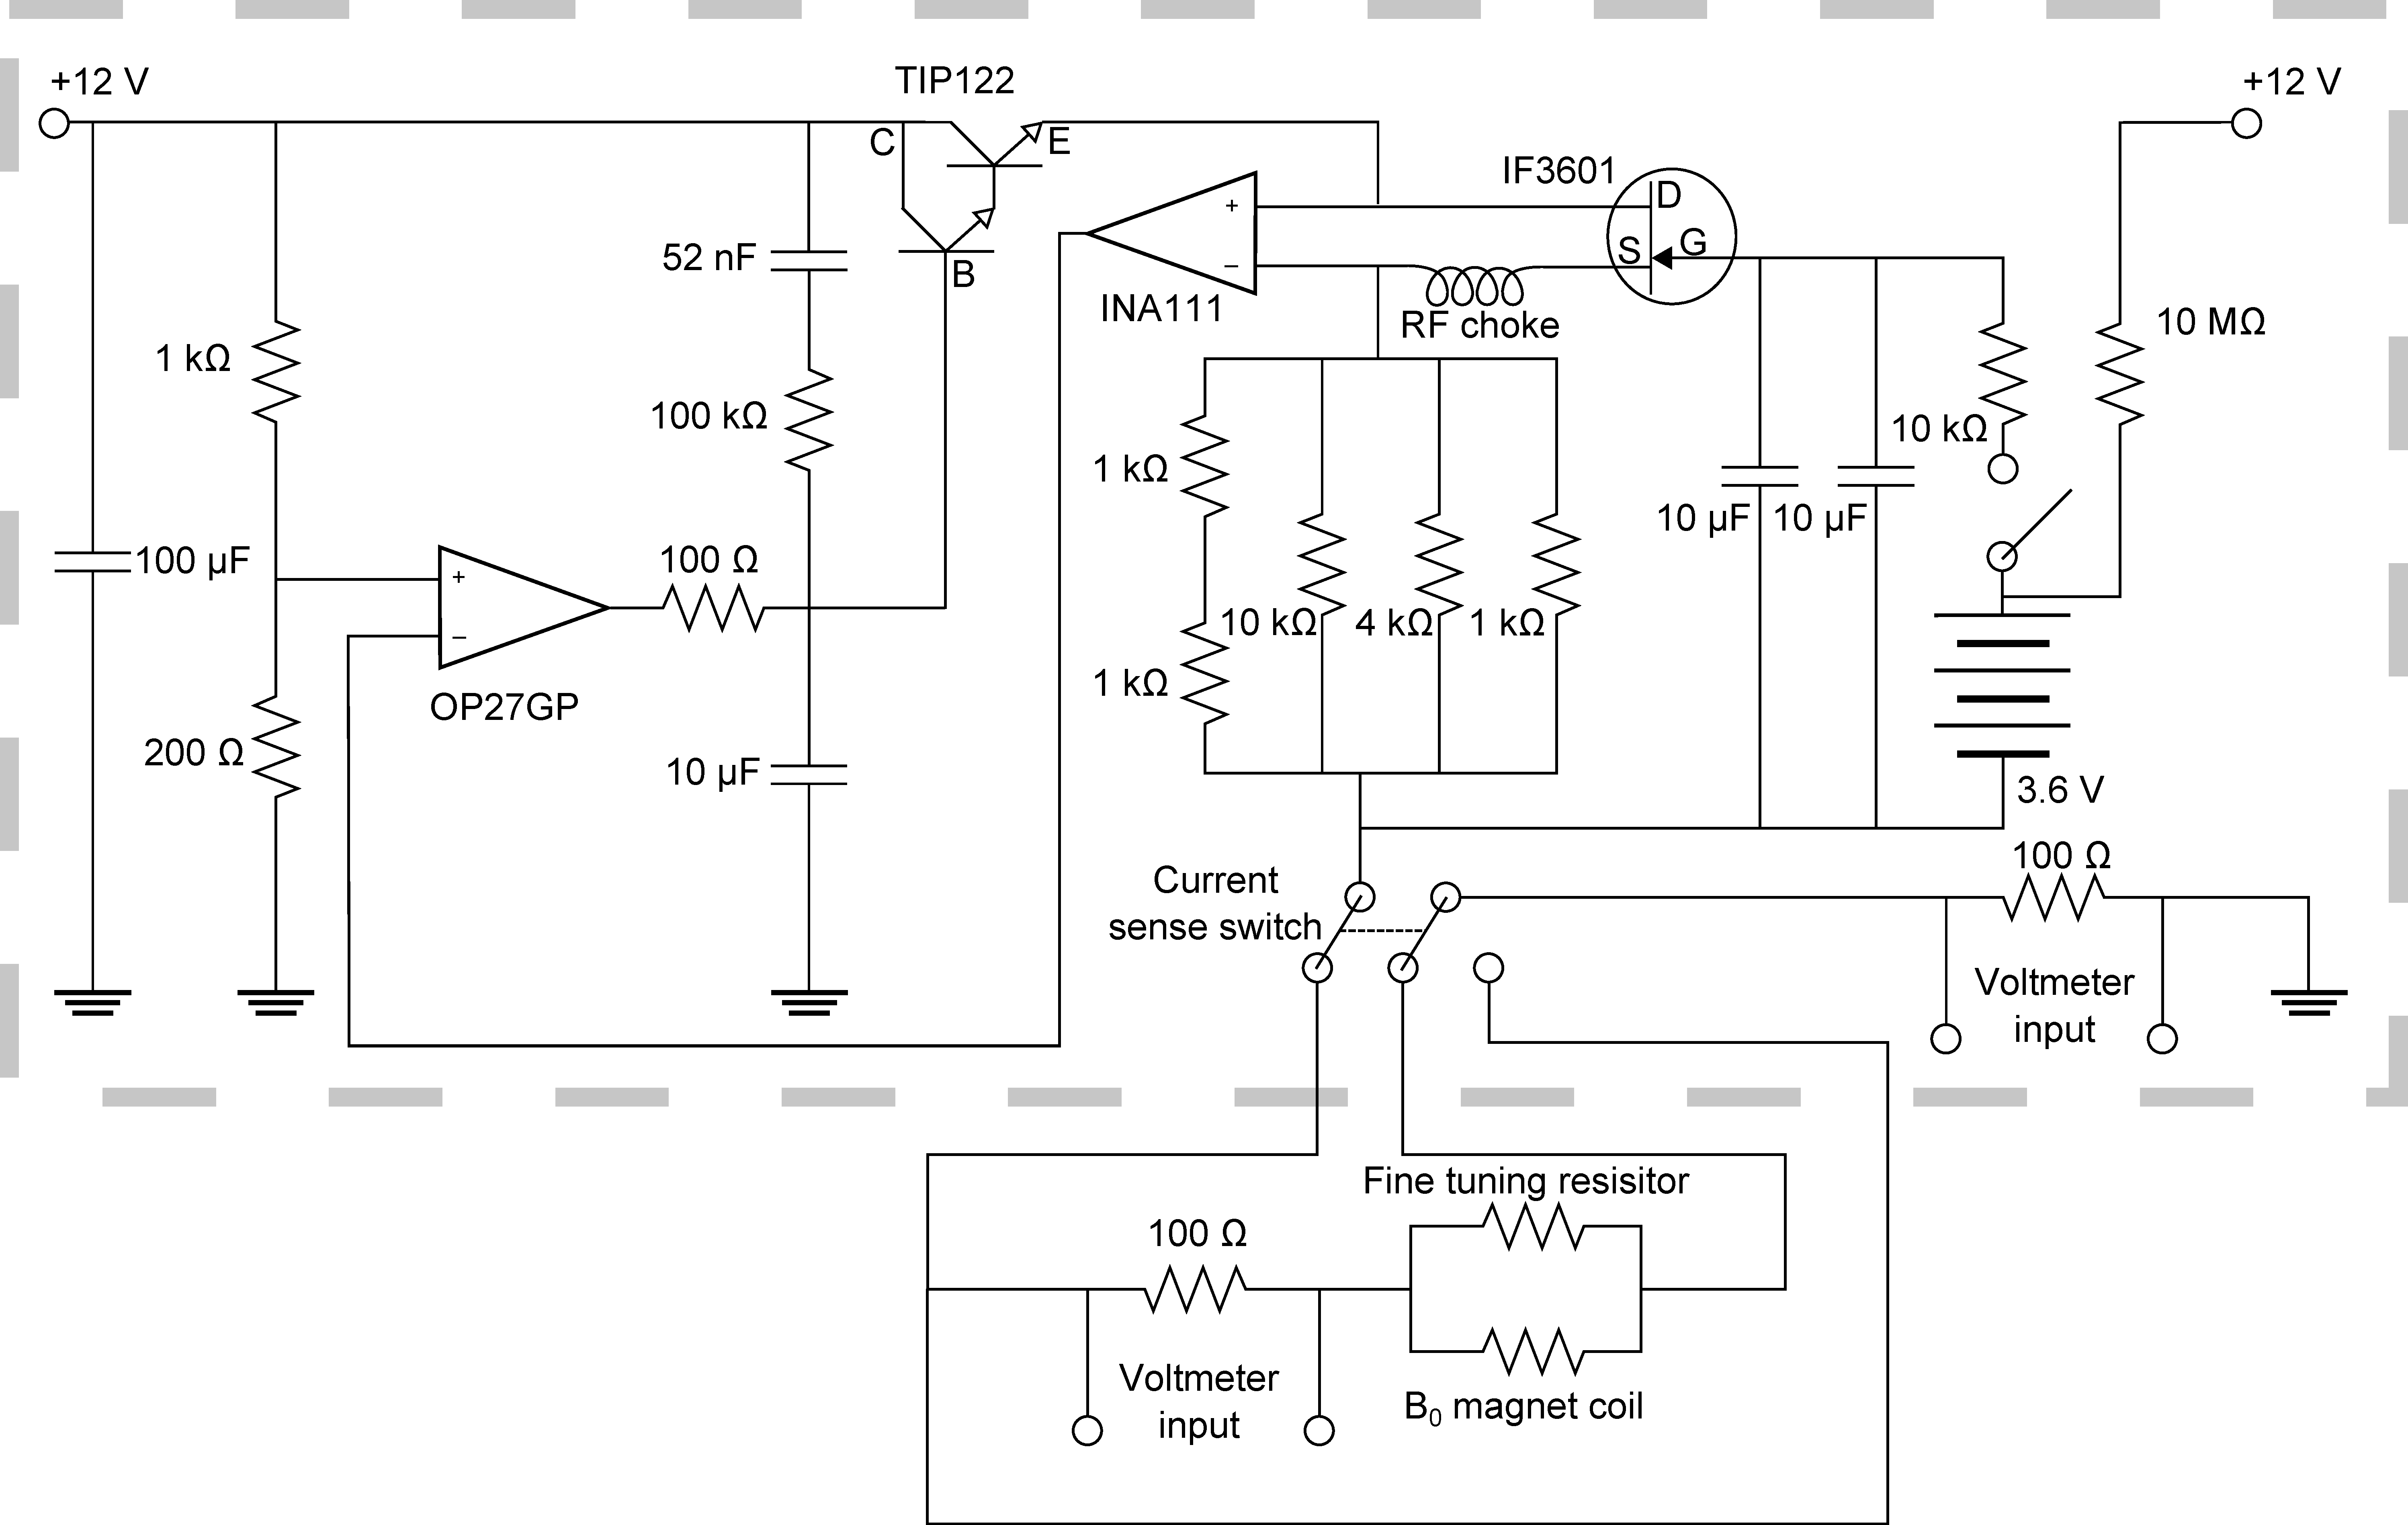
\includegraphics[scale=0.14]{Figures/B0_Source_Circuit_Diagram.pdf}
\end{center}
\caption[$\mathbf{B}_0$ current source diagram]{\narrower A simplified diagram of the circuit used to provide current to the main magnet coil. The circuit uses a lithium battery (3.6 V) as a low-noise voltage reference to regulate the current through the JFET. The dominant source of noise in the circuit is thermal fluctuations of the JFET, so the circuit is housed in a polystyrene foam box filled with packing peanuts (indicated by the dashed line) to minimize changes in air circulation patterns. Power connections for the two op-amps and the -12 V rail are not shown.}
\label{Italian_Source_Diagram}
\end{figure}
A feedback loop is used in the circuit to maintain $V_{DS}$ at approximately 2 V. The INA111 has unit gain and outputs $V_{DS}$ to the (high-gain) OP27GP. The OP27GP compares the value of $V_{DS}$ at the inverting input to the set point formed by the voltage divider at the non-inverting input, and adjusts the voltage at the drain of the JFET with the Darlington transistor TIP122. 

The use of a battery voltage reference controls the noise from the supply but also introduces an additional obstacle: even when it supplies no current to the circuit, the battery can `self-discharge' over long time scales. Because the data analysis method relies on matching the Larmor precession period to the the data sampling time interval,\footnote{Specifically, the current through the magnet coil is tuned to keep the precession period of the atoms near 120 ms to optimize the effectiveness of the digital filters, described in detail in section \ref{Digital_filter}.} and the current $I_S$ controls the Larmor frequency, a slow decline in the battery voltage will adversely impact the performance of the experiment. To avoid voltage droop from the battery over months of continuous operation, a small current is fed into the battery from the positive rail via a 10 M$\Omega$ resistor.

The average value of $\mathbf{B}_0$ was fine tuned by adding a wire-wound resistor in parallel with the magnet coil to draw off excess current from the supply. This additional resistor was not thermally insulated, and the second-order gradient coil $\partial B_y/\partial y^2$, run in series with the main coil, had a similar parallel resistor with a much higher temperature coefficient. Temperature changes can thus change the fraction of $I_S$ which travels through the magnet coils, adding more noise to the magnetic field than the current fluctuations from the supply can account for. This is consistent with observations of the noise level on the average precession frequency in comparison to the noise on the current supply. These external resistors were therefore likely to be the dominant source of noise in the magnetic field environment and have been removed for the next round of EDM data.

\begin{figure}
\begin{center}
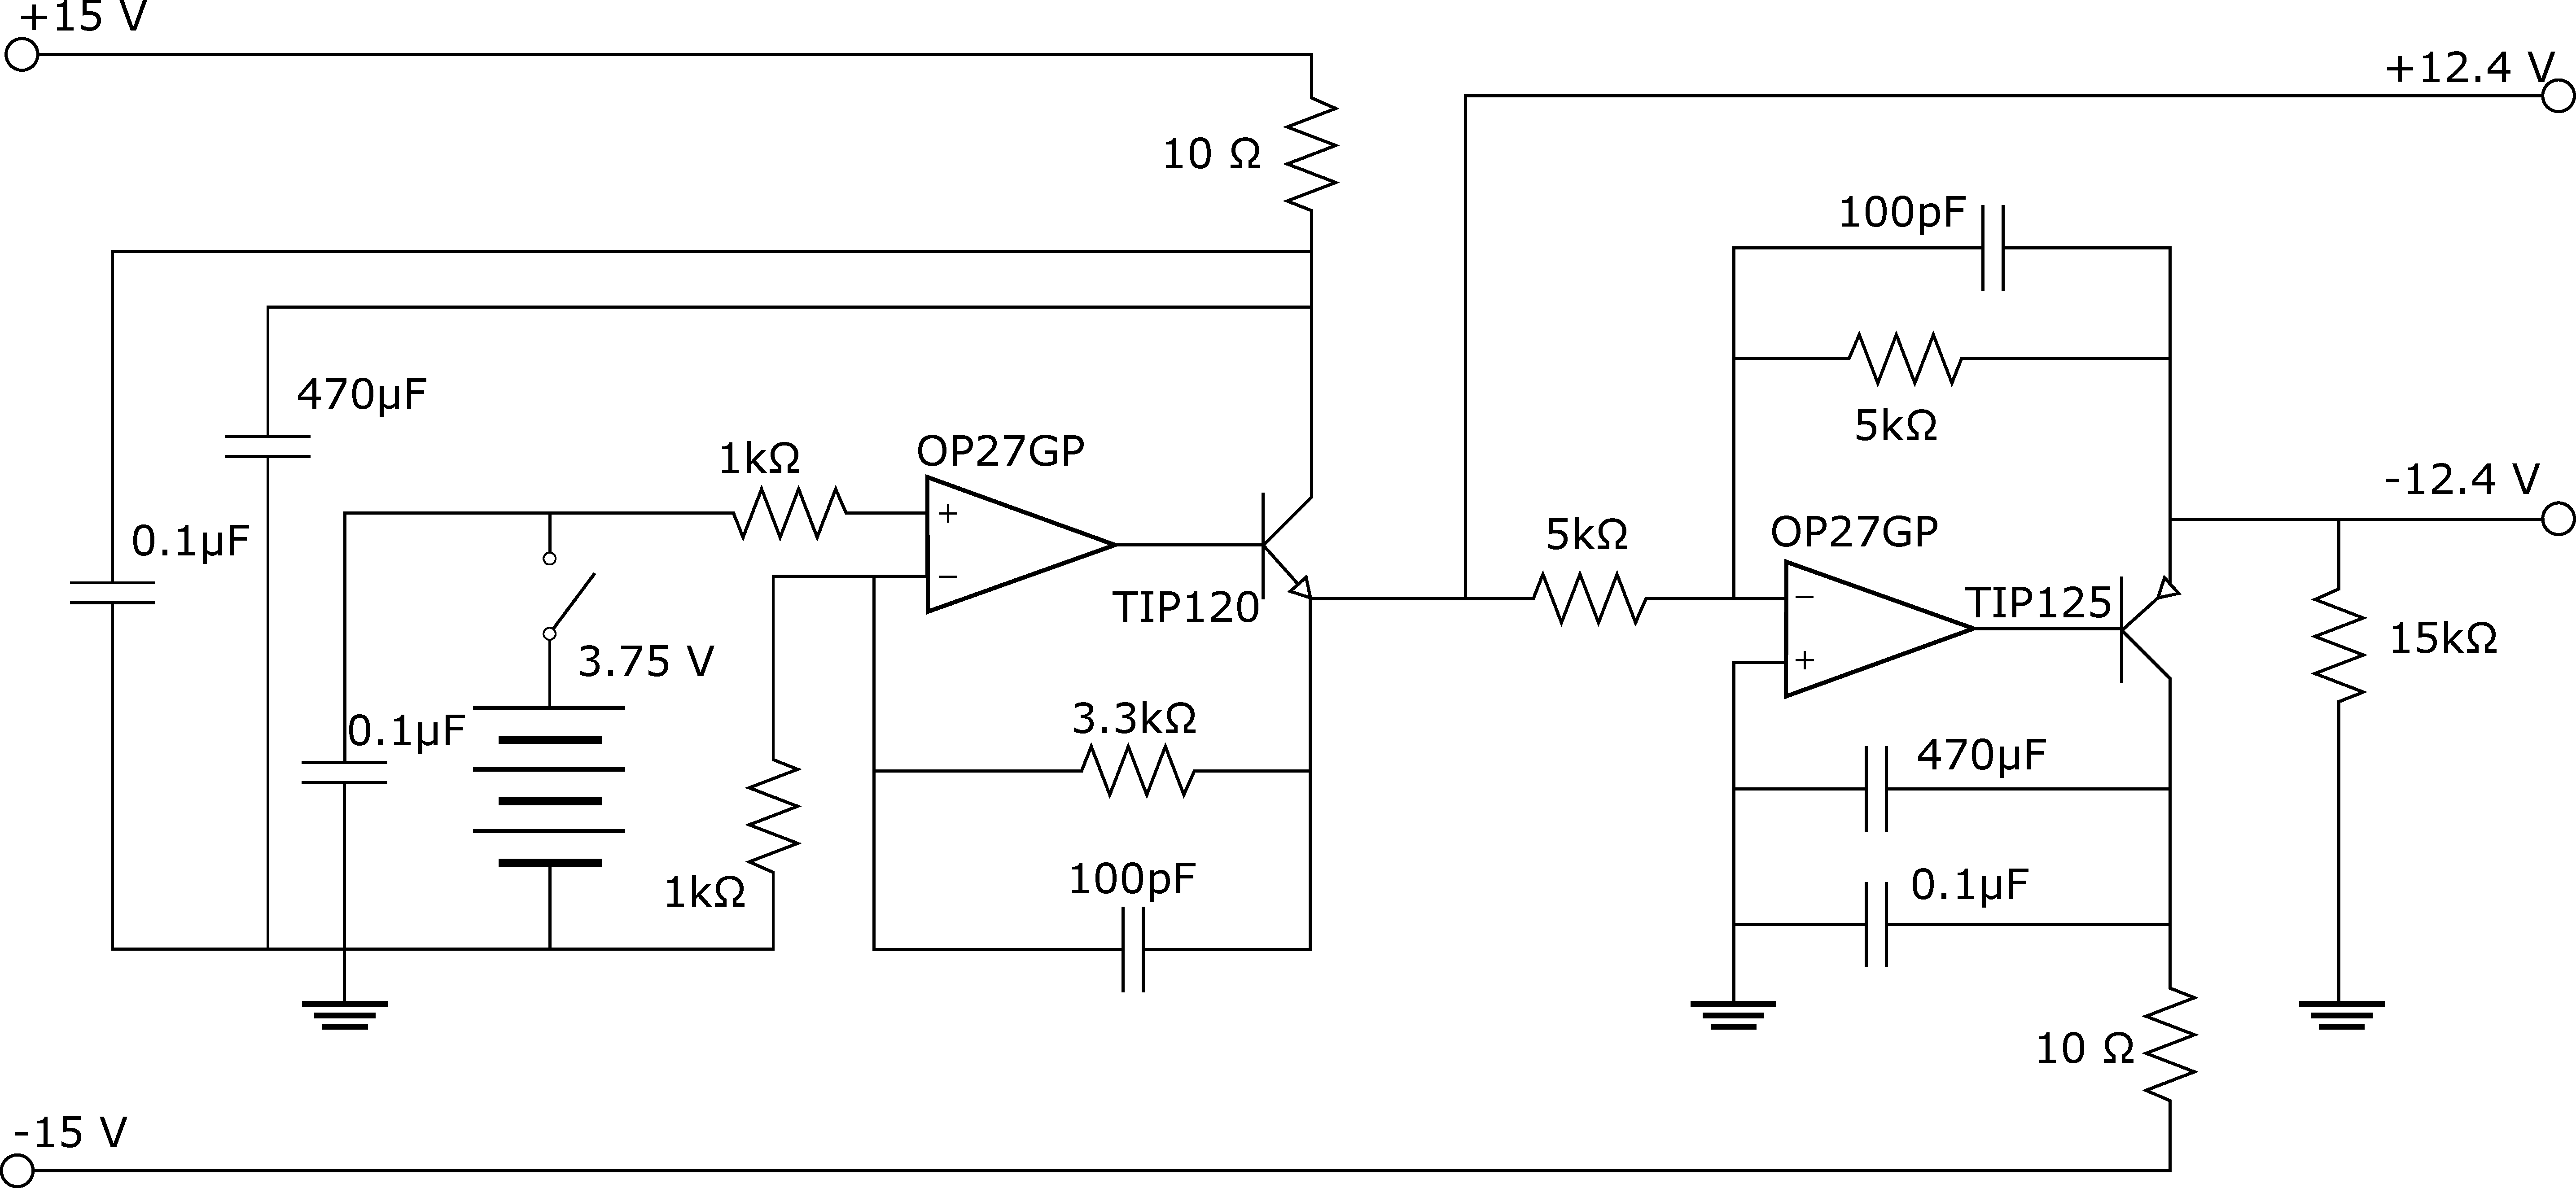
\includegraphics[scale=0.14]{Figures/B0_Current_Source_Power_Supply.pdf}
\end{center}
\caption[$\mathbf{B}_0$ power supply diagram]{\narrower A diagram of the circuit used to provide $\pm$12 V to the main coil current source. As with the circuit in Figure \ref{Italian_Source_Diagram}, a battery voltage reference is used as input to an op-amp/transistor output. In this case, the battery is a set of three nickel-cadmium 1.25 V C-cells. Power connections for the two op-amps are not shown.}
\label{Italian_Source_Power_Supply}
\end{figure}

\subsection{Magnetic shielding}
The vessel and magnet coil sit inside a set of three nested cylindrical shields (with diameters of 12", 18", and 24") of 0.75 mm thick mu-metal, an alloy with weak-field magnetic permeability $\mu \geq 4\cdot10^4$. The axis of the shields is oriented in the horizontal direction. Circular endcaps are press-fit on either side, overhanging the cylinder bodies by 4". The endcaps have 4" holes to allow magnet wires, HV cables and leakage current wires to reach the vessel and magnet coil. Smaller 1.25" holes in the cylinder walls halfway between the endcaps permit access for the middle-cell laser beams, and 1.25" holes in the bottom and at the midline are used for support rods that hold the inner shields and magnet coil assembly in the center of the outermost shield. 

For frequencies $\omega$ such that the skin depth $c/\sqrt{2\pi\mu\sigma\omega}$ is greater than the thickness of the material, the shielding effect is caused by the propensity of the high-$\mu$ material to concentrate lines of magnetic flux in the bulk, directing them away from the enclosed volume \cite{Jackson}. In a uniform static field $\mathbf{B_{ext}}$, the shielding factor $S$ relates the strength of the field inside the shield $\mathbf{B_{int}}$ to that of the (unperturbed) field outside. For a single cylinder of radius r, thickness $t$, and permeability $\mu$, the shielding factor for external fields perpendicular to the shield axis is
\begin{equation}
S_T = \dfrac{\mathbf{B^{\bot}_{int}}}{\mathbf{B^{\bot}_{ext}}} \approx \dfrac{2r}{t\mu}.
\end{equation}
For fields along the shield axis, the shielding factor depends on the ratio of shield length to radius. The shields used in the EDM experiment are approximately 4 times the legth of the radius, so the axial shielding factor is \cite{Khriplovich_Lamoreaux}
\begin{equation}
S_A = \dfrac{\mathbf{B^{\parallel}_{int}}}{\mathbf{B^{\bot}_{ext}}}  \approx \dfrac{4r}{t\mu}.
\end{equation}
The shielding factor of a nested set of shields is superior to that of a single shield with the same total thickness; for a set of $n$ nested shields, the total shielding factor $S_{tot}$ can be approximated by
\begin{equation}
S_{tot} \approx S_n \prod_{i-1}^{n-1} S_i\big(1-(\dfrac{X_{i+1}}{X_i})^k\big)^{-1},
\end{equation}
where $S_n$ is the shielding factor of the outermost shield, $S_i$ is the shielding factor of the $i$th shield, and the product runs from the largest to the smallest shield (i.e., $X_{i+1} < X_i$). The parameter $k$ is different for various shield geometeries and field orientations: for a cylindrical shield, k is approximately 2 if the external field is perpendicular to the shield axis, while k decreases to approximately 1 for fields parallel to the axis \cite{MagShielding}. Thus, while the axial shielding factor appears greater than that of the transverse shielding factor of a single cylinder, the combined set of three cylinders shields transverse fields more effectively. The measured shielding factor of the EDM setup is approximately 50,000 in the transverse direction, and approximately 5000 in the axial direction.

Each time the shield endcaps are moved or the internal field generated by the magnet coil is changed, the shields are degaussed by applying a low-frequency oscillating current to a coil which is wound toroidally down the shield axis and around the outside. The flux generated by the degauss current should initially be enough to drive the mu-metal to saturation, after which the amplitude of the degauss waveform is slowly decreased until the shields relax to the ambient field. The saturation flux for the EDM shield setup is approximately 100 amp-turns. In practice, the shields are degaussed with a 5 Hz waveform input to a KEPCO bipolar power supply, which is output to a 1:1 isolation transformer followed by an 8-turn coil. The 5 Hz carrier waveform is exponentially attenuated with a typical relaxation time of 30 s for a total degauss time of 5 minutes. To avoid transient currents which may re-magnetize parts of the shields after degaussing, the coil connection is manually broken before disengaging the power supply. 

Investigations of the magnetic field gradients inside the shields indicated that the degauss proceedure as described above generates irreproducible gradients. This behavior is undesireable for minimizing systematics associated with motion of the cells in a non-uniform field, so more consideration of the degauss proceedure is warranted in the future. Spacing out individual strands of the degauss cable around the rim of the shields may yield a more uniform field \cite{Fierlinger}, though attempts to incorporate this method into the EDM setup have not improved reproducibility. In addition, an asymmetry in the output current waveform would generate harmonics of the 5 Hz carrier which could interact with the magnetization of the shields, leaving them in a variable state between degausses. Such an asymmetry may be induced by the bit noise on the output waveform, a non-linearity in the power supply, or some residual permanent magnetization  of the isolation transformer. 

\subsection{HV supply} 
To avoid introducing potential systematics, it is vital to prevent the high voltage from influencing the precession signal data in any way except through the interaction of $\mathbf{E}$ and a non-zero EDM. To this end, the HV supply is controlled by a separate computer from the EDM data acquisition setup, and is magnetically shielded to prevent fields generated by the supply from altering the field seen by the vapor cells. The HV supply and HV computer are also located in another room approximately 10 m from the EDM computer, isolated by an optoelectronic link so that no electrical signals travel directly between them. The EDM data acquisition computer outputs a TTL pulse each time a new pump-probe cycle is initiated; all available information about the state of the electric field is controlled and recorded in real time only by the HV computer. The high voltage is set by a $\pm$10 V input to an Applied Kilovolts model HP010R, the output of which is monitored using a 1000:1 voltage divider and digitized along with the electrometer outputs at 2 Hz. The HV computer is typically programmed to reverse the voltage polarity each time it receives a TTL pulse from the EDM computer, after which it begins ramping the voltage and recording displacement/leakage currents deposited on the groundplane.

\section{Leakage currents} \label{Leakage_methodology}
In previous iterations of the experiment, the most pernicious EDM-like effects were driven by the small electric currents which flow from the high voltage electrodes to ground. Such currents would necessarily reverse with the polarity of the HV, along with the direction of the associated magnetic field $\mathbf{B}_{leak}$. While currents which follow the electric field lines can only induce a $\mathbf{B}_{leak}$ which points in the horizontal direction (and thus adds quadratically to $\mathbf{B}_0$), any helicity in the currents would create a $\mathbf{B_{leak}}$ that adds linearly with $\mathbf{B}_0$. Only the projection of $\mathbf{B}_{leak}$ onto $\mathbf{B}_0$ is of concern to the systematic error budget. 

\begin{figure}
\begin{center}
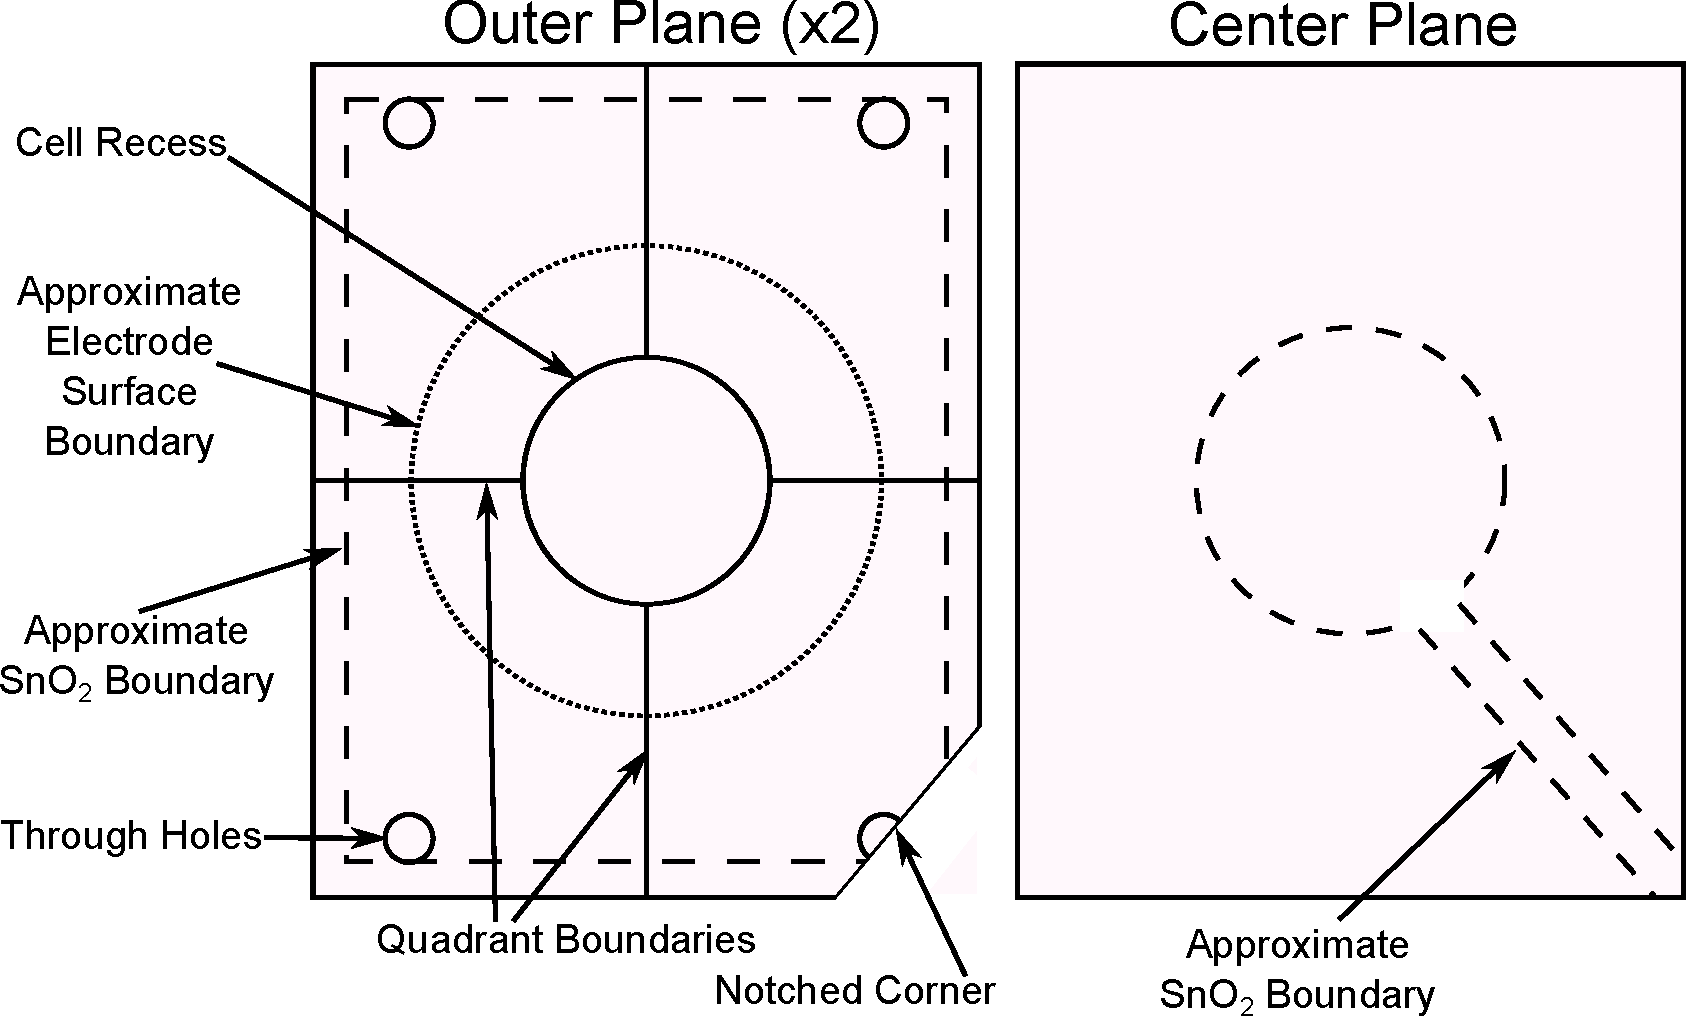
\includegraphics[scale=0.4]{Figures/Groundplane.pdf}
\end{center}
\caption[Scale drawing of fused silica groundplane]%
{\narrower A scale drawing of the groundplane dividing the two halves of the EDM vessel. Left: a view of the outer groundplane layers. The dashed line indicates the approximate boundary of the SnO$_2$-coated area. One corner is cut off of each outer groundplane layer to facilitate leakage current connections to the inner layer. Right: the innner groundplane layer, with SnO$_2$-coated area indicated. Leakage current measurements from this channel are assumed to flow down the cell surface.}
\label{GroundplaneDiagram}
\end{figure}

To collect the leakage currents, the outer surfaces of the groundplane are coated with semi-conductive tin(IV) oxide (SnO$_2$). The procedure followed for preparing the coating is based on the one described in \cite{Griffith}. The glass is cleaned in an ultrasonic bath with soap and water, followed by de-ionized water and a 5\% solution of hydrochloric acid (HCl) to remove ferrous metal contaminants. After cleaning, the glass is heated to 425 $^{\circ}$C, using an oven connected to a fume hood, then sprayed with a solution of 5 parts ethyl alcohol to 1 part tin chloride (SnCl$_4$) by mass. The SnCl$_4$ reacts with O$_2$ to form the SnO$_2$ coating. After several coats of tin oxide, the typical resistance between any 2 points on the piece is less than 15 k$\Omega$. To eliminate helical currents around the base of the cells, a narrow strip was painted over with a paste made from alumina polishing powder during application of the final coats of SnO$_2$, leaving the area covered with a relatively thin layer and increasing resistance between the 4 quadrants. Leakage current wires are attached to all four quadrants near the corners of the outer groundplane layers to draw current radially away. Leakage current wires from the four quadrants on top and bottom are soldered together outside of the vessel walls so all the currents reaching the outer top portion are measured together, and similarly for the outer bottom. 

\begin{figure}
\begin{center}
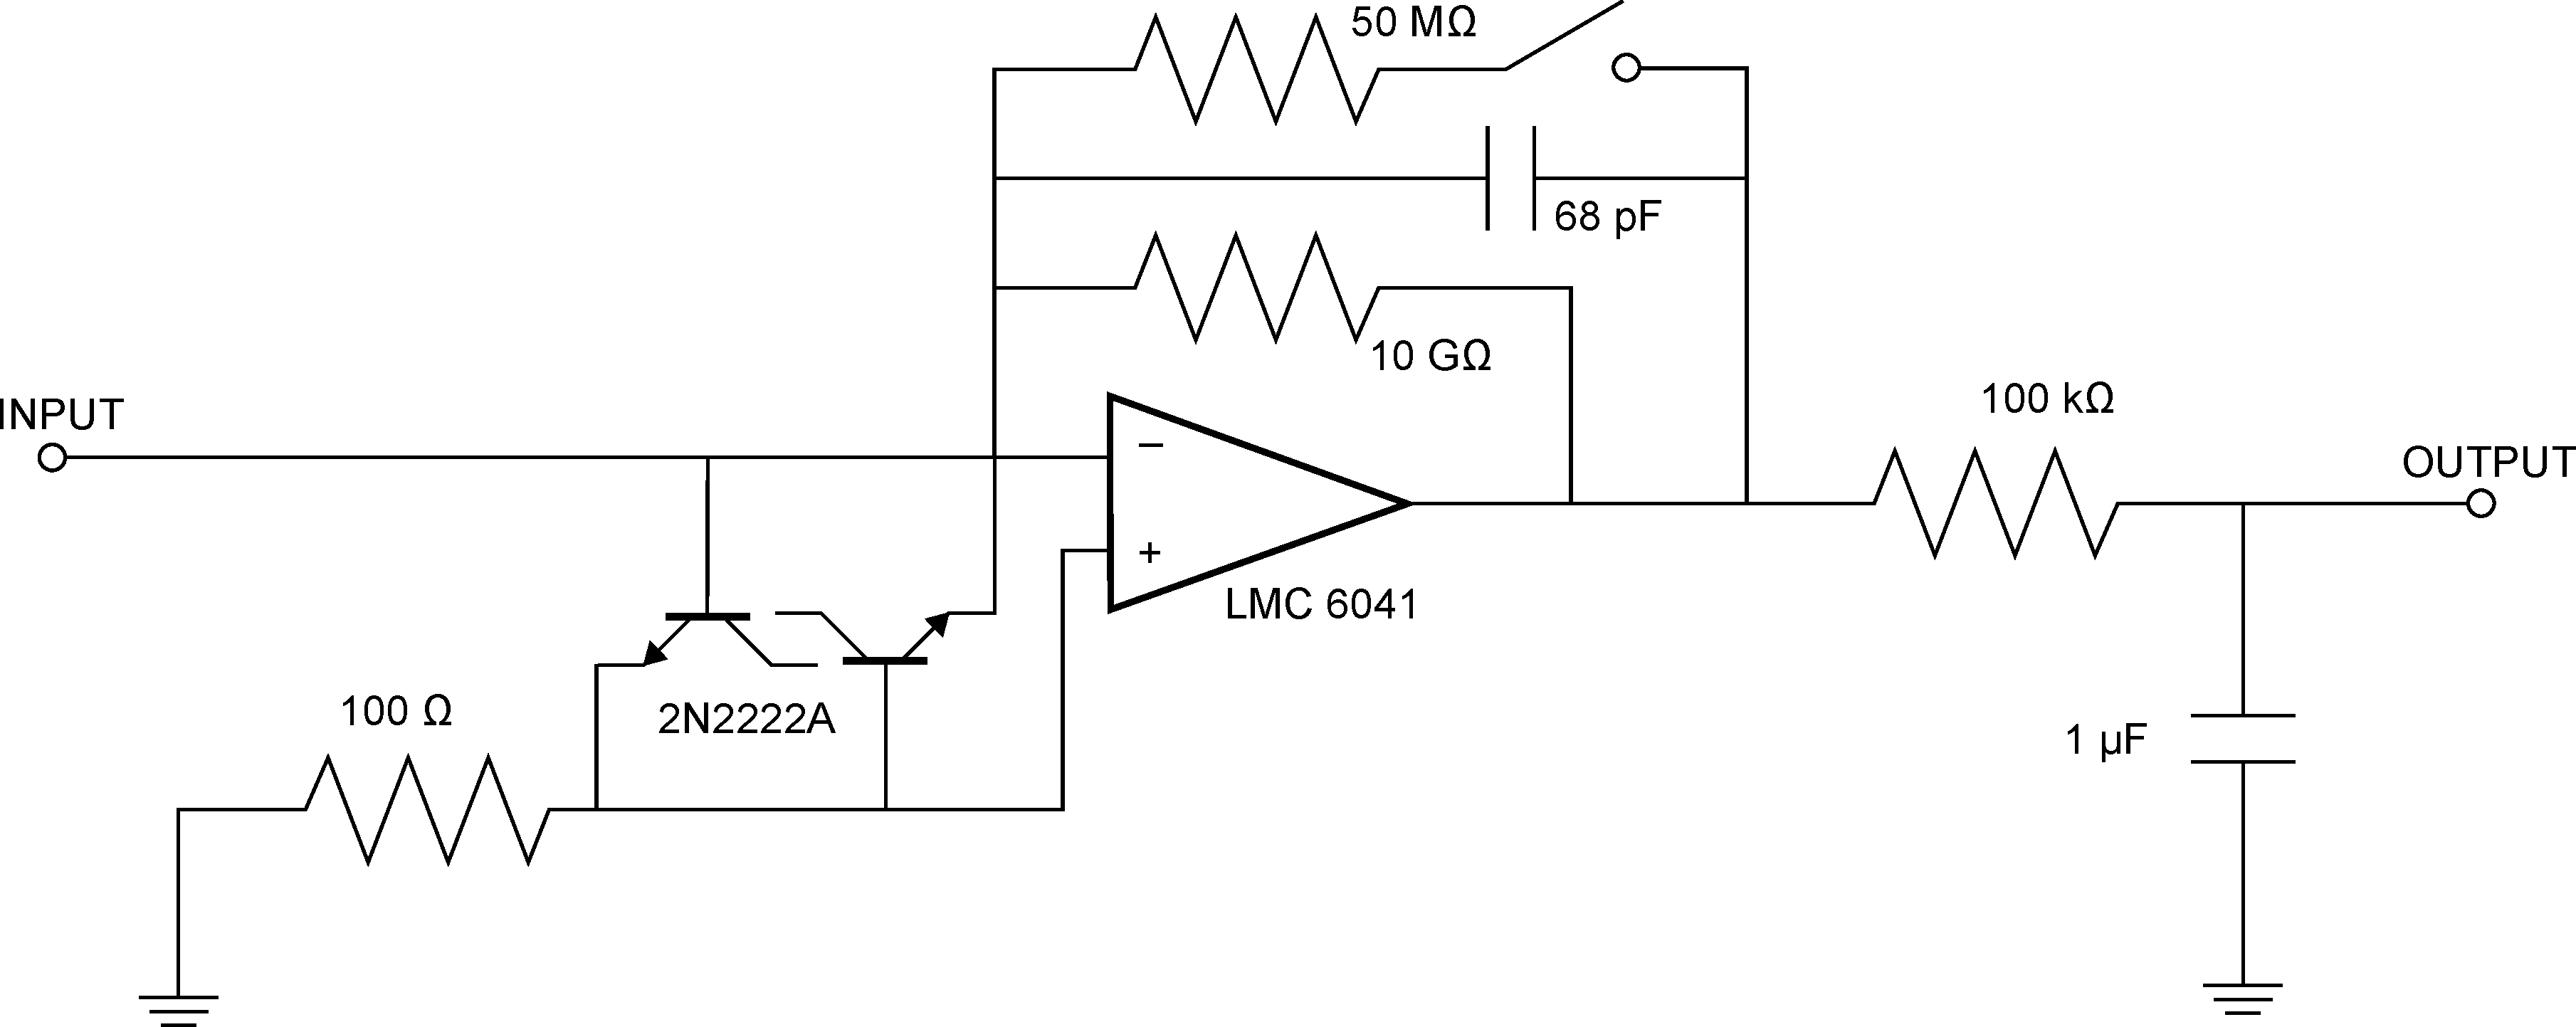
\includegraphics[scale=0.17]{Figures/Electrometer_Circuit_Diagram.pdf}
\end{center}
\caption[Circuit diagram of leakage current monitors]
{\narrower A simplified diagram of the circuit used to monitor leakage currents flowing from the vessel walls and groundplane. The input is a virtual ground, and the potential difference across the gain resistor corresponds to the voltage drop due to the input current. The connection to the inverting input pin is air-wired to prevent the small input currents from escaping across the component surfaces. The base-emitter junctions of the 2N2222A transistors function as protection diodes by shunting current to ground in the event of a spark or other discharge; the collector pins have no connections.}
\label{ElectrometerDiagram}
\end{figure}

The currents flowing from electrodes to the groundplane are monitored with variable gain transimpedance amplifiers. The circuit diagram is shown in Figure \ref{ElectrometerDiagram}. The leakage current monitors are based on LMC6041 CMOS op-amps with an ultra low input-offset current ($\leq$0.25 fA). During the high voltage ramp, the HV computer outputs a TTL signal that closes the reed relay switch so displacement currents are measured with 5\% of the normal gain. The switch is then opened to measure the leakage currents at high gain. 

Leakage currents recorded on the outer portions of the groundplane flow from the electrode surface to ground through the air. The air inside the vessel is assumed to be homogeneous, so the electric field lines cannot have any associated helicity-only charges moving down the cell walls can flow in a helical pattern. Helical current paths may be supported by the internal structure of the cell walls or external impurities adsorbed onto the (inner or outer) glass surface. The bulk resistivity of the Heraeus Suprasil used to fabricate the cell bodies is quoted as $10^{18}$ $\Omega \cdot$cm. An EDM cell body is 1 cm long and has a cross-sectional area $\approx$ 1 cm$^2$, which would form a resistor of $10^{18}$ $\Omega$. This would yield an expected leakage current of $10^{-14}$ A with a potential difference of 10 kV, several times less than the observed leakage currents. Therefore, currents collected on the inner layer of the groundplane are assumed to flow down the cell surfaces (although there is a current path through the gas between cell endcaps which will deposit charges on the inner groundplane). These currents are assumed to be the only ones which contribute to a potential systematic shift of $\Delta\omega_{EDM}$. 

\begin{figure}
\begin{center}
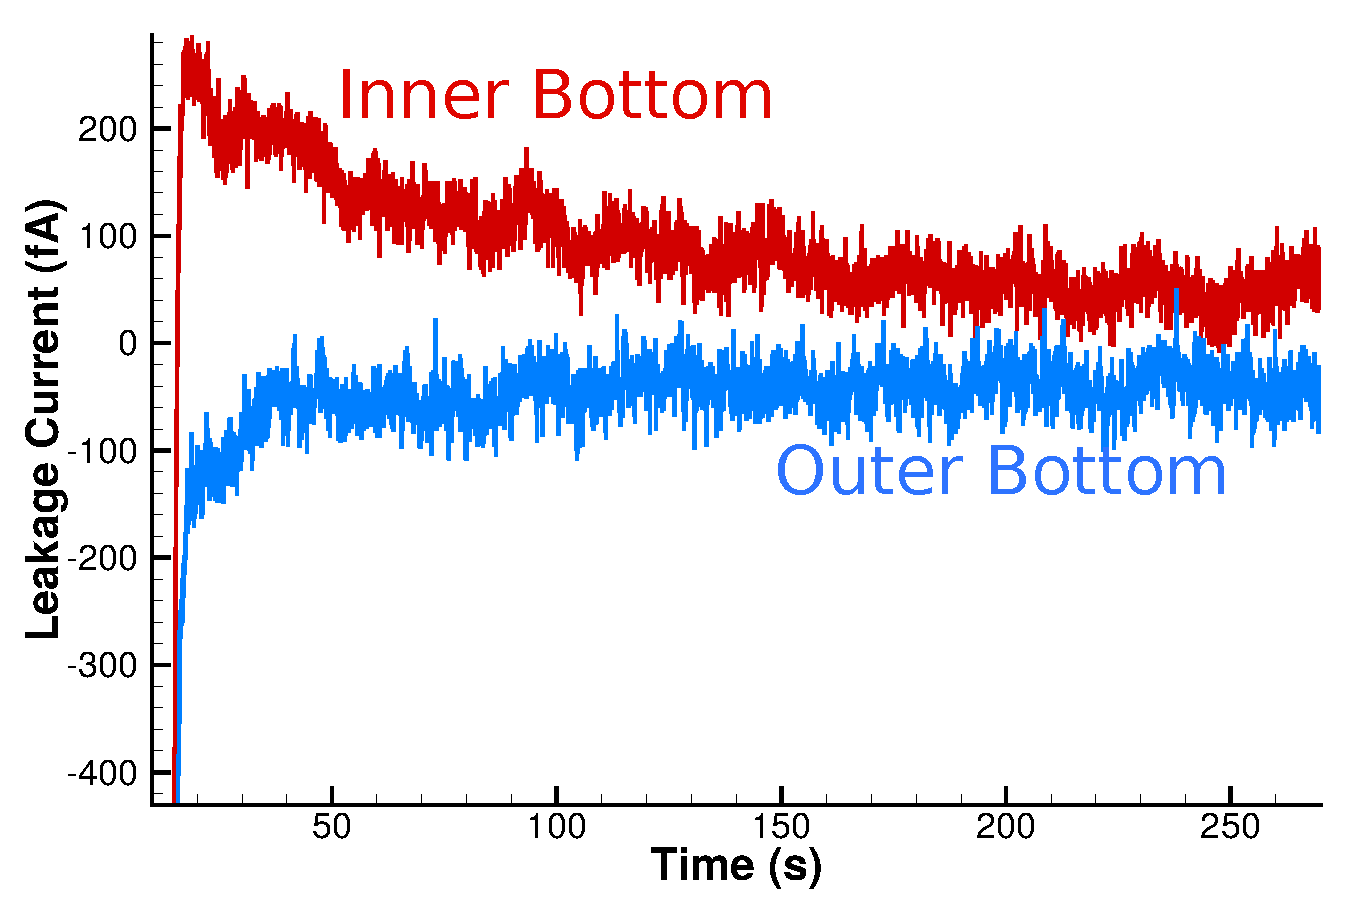
\includegraphics[scale=0.5]{Figures/IB_OB_Leakage_Current.pdf}
\end{center}
\caption[Bottom Side Leakage Currents]
{\narrower The leakage currents collected on the bottom side of the groundplane during a typical run (\#72047) following the high voltage ramp and gain switch. The inner bottom current appears to be flowing opposite the applied electric field, likely due to dielectric absorption in the cell walls.}
\label{IB_OB_Leakage_Current}
\end{figure}

While the instrumentation is sensitive enough to resolve currents on the order of fA, the "real" leakage currents are easily overwhelemed by spurious effects inside the vessel driven by the HV. Figure \ref{IB_OB_Leakage_Current} illustrates the behavior of the leakage current monitors on the bottom side of the groundplane during a normal run. The inner portion of the bottom side records a current that begins negative and passes through 0, behavior which is not consistent with leakage current from the high voltage electrodes to ground. However, the effect persists with a time constant on the order of several hundred seconds, which is consistent with the buildup and dissipation of space charges inside the bulk of the fused silica \cite{2010_LIGO_Fused_Silica_Space_Charge}. This phenomenon is also known in electronics as dielectric ``leakage" or ``soakage", whereby a shorted capacitor fails to fully discharge and recovers a measureable voltage over time if the current path between the terminals is not maintained. This behavior, combined with the extremely high resistivity of the fused silica, can explain the currents which appear to flow in the direction opposite the applied voltage.

Odd behavior of the leakage currents can also be observed in channels which appear to be mirror images on one another. Figure \ref{IT_OT_Leakage_Current} shows the charging and leakage currents recorded on the top side of the groundplane during the same run as Figure \ref{IB_OB_Leakage_Current}. Leakage currents on both the inner and outer portions of the groundplane should be of the same sign as the charging currents, but a coupling between the plates causes current to be sourced from one to the other, making mirror image signals on the elecrometers. The currents likely originate from a difference in the electrometer input offset voltages, which allows one electrometer to source current to the other through the finite resistance between inner and outer parts of the groundplane.

\begin{figure}
\begin{center}
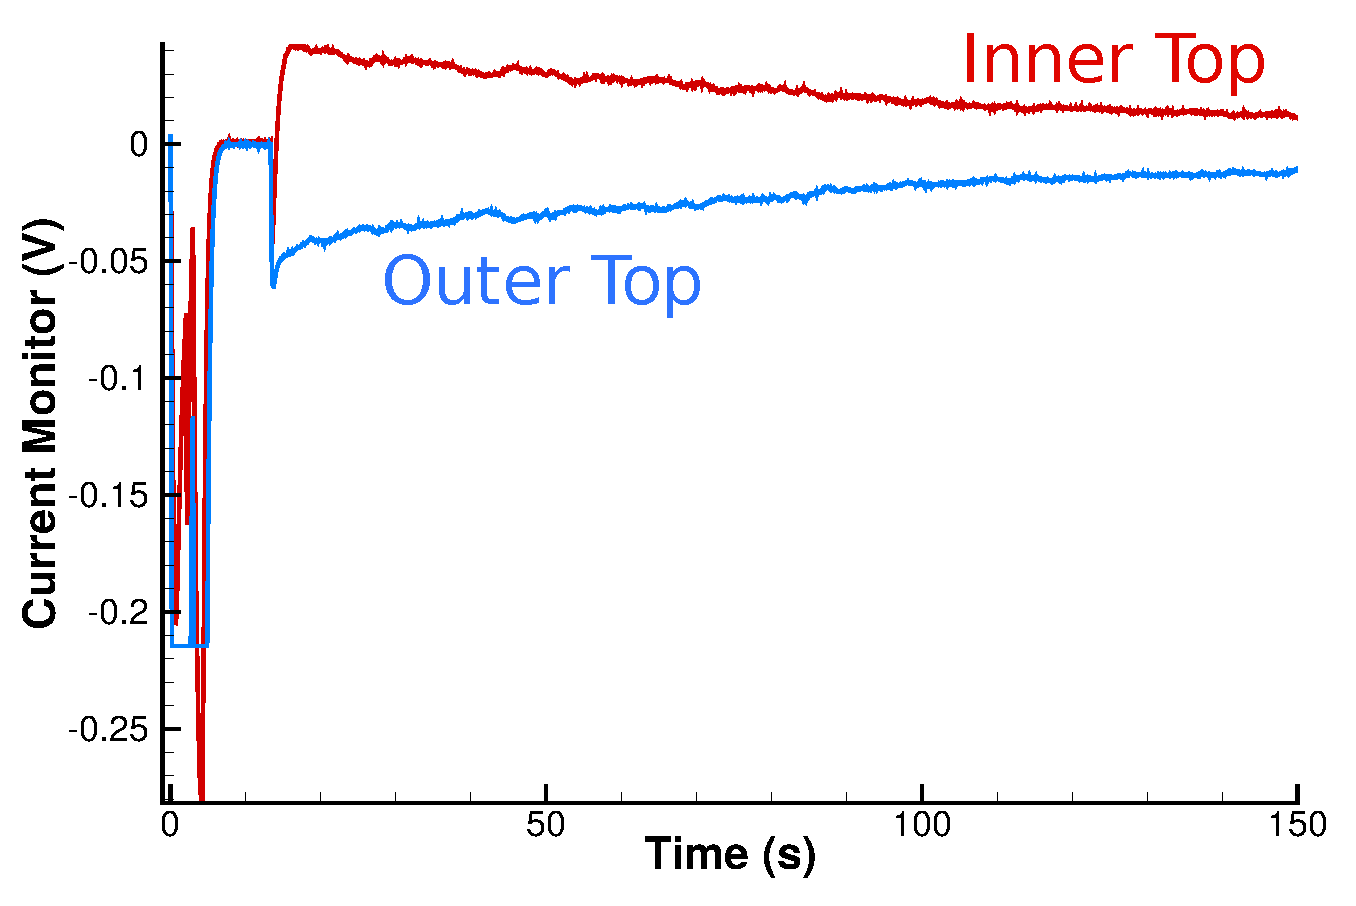
\includegraphics[scale=0.5]{Figures/IT_OT_Leakage_Current.pdf}
\end{center}
\caption[Top Side Leakage Currents]
{\narrower A truncated view of the first 150 s of current monitor data for a typical run (\#72047). The high voltage ramp lasts for 15 s and includes a brief pause while the polarity is flipped. During the ramp, the gain resistor is $50\text{ M}\Omega$. Following the high voltage ramp, the gain resistor is swtiched to $10\text{ G}\Omega$, and the electrometer reading increases accordingly. Coupling between the two electrometer input offset voltages allows one electrometer to source current to the other through the groundplane. }
\label{IT_OT_Leakage_Current}
\end{figure}	

While the effects of electrometer coupling and dielectric soakage due to space charge persist much longer than a typical pump/probe cycle of the Hg atoms, they do settle into a steady state after several thousand seconds, after which all the electrometers indicate currents $\le 40$ fA flowing in the expected direction. Obviously, this steady-state value of the leakage currrent was not recorded with each run, but the approximate values can be used to estimate the leakage current systematic in Chapter \ref{leakage_systematic}.

\section{Signal acquisition and conditioning}
The polarization rotation angle of the beam after exiting each cell is observed using a Wollaston prism and a pair of photodiode amplifiers. The signal on the two photodiodes is balanced by means of a zero-order $\lambda/2$ waveplate located in front of the Wollaston prisms. The precession signal from each cell is taken to be the difference in the two photodiode intensities $I_s$ and $I_p$, normalized by the total intensity $I_s+I_p$. 

Each polarization state is detected by a 5 mm$^2$ UV-enhanced photodiode (UDT sensors model UV-005). The diodes have 100\% internal quantum efficiency, making them well-suited for low-intensity applications. Each photodiode sits at the focus of a 25 mm lens, which is mounted on a 2-axis translationstage to maximize the light collection efficiency. The protective quartz windows are removed from the diode housings to prevent reflection and etaloning. 
\begin{figure}
\begin{center}
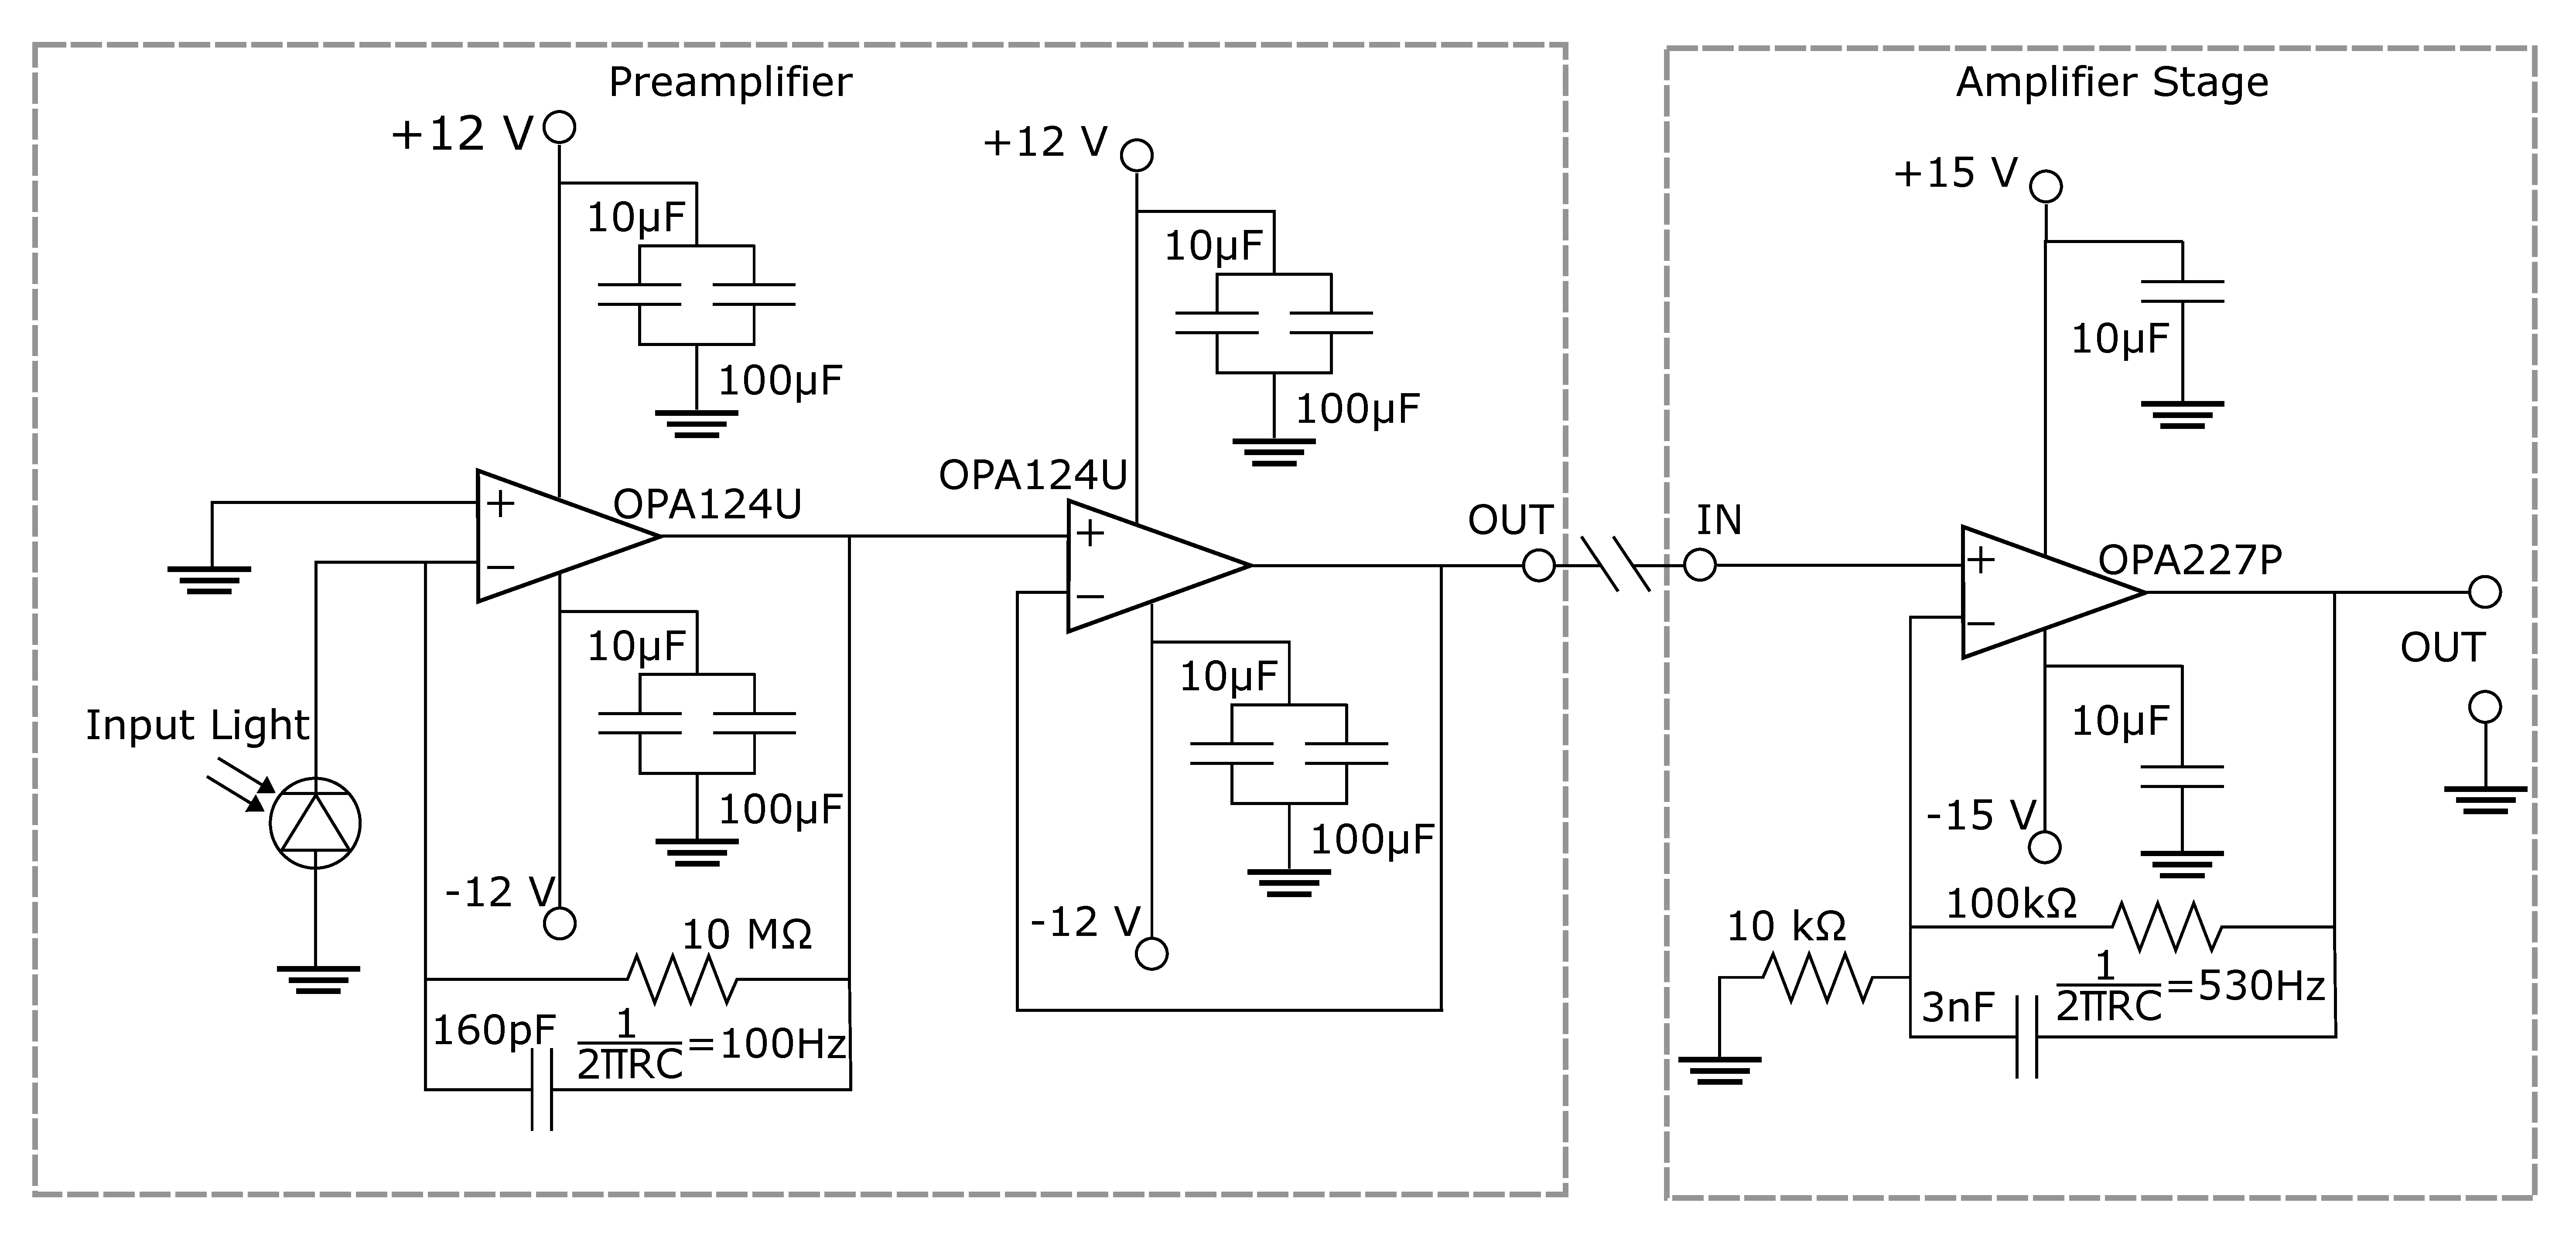
\includegraphics[scale=0.15]{Figures/Pre+amplifier.pdf}
\end{center}
\caption[Photodiode amplifier circuit]{\narrower A diagram of the circuit used to amplify the current signal from the UV silicon photodiode detectors. The preamplifier stage includes the unbiased photodiode and a 100 Hz lowpass filter, with a follower to boost output impedance. Only the part of the amplifier circuitry with 10x gain is shown; the other gain circuits are identical up to the ratio of the two gain resistors at the bottom.}
\label{Amplifier_Diagram}
\end{figure}

The photodiodes are operated without reverse bias in the photovoltaic mode. Eight preamplifier circuits housed inside the mounting boxes for the photodiode/lens assembly ensure that signals travel no more than 50 mm before amplification. The preamplifier circuit is illustrated in Figure \ref{Amplifier_Diagram}. After the preamplifier, the signals travel through approximately 3 meters of coaxial shielded cable to the amplifier stage. The amplifier has 24 total channels, each of which includes a 530 Hz filter. Amplifier channels are divided into three groups, with gain factors of 5, 10, or 20. The amplifier outputs are insulated BNC jacks, which are measured differentially.
\begin{figure}
\begin{center}
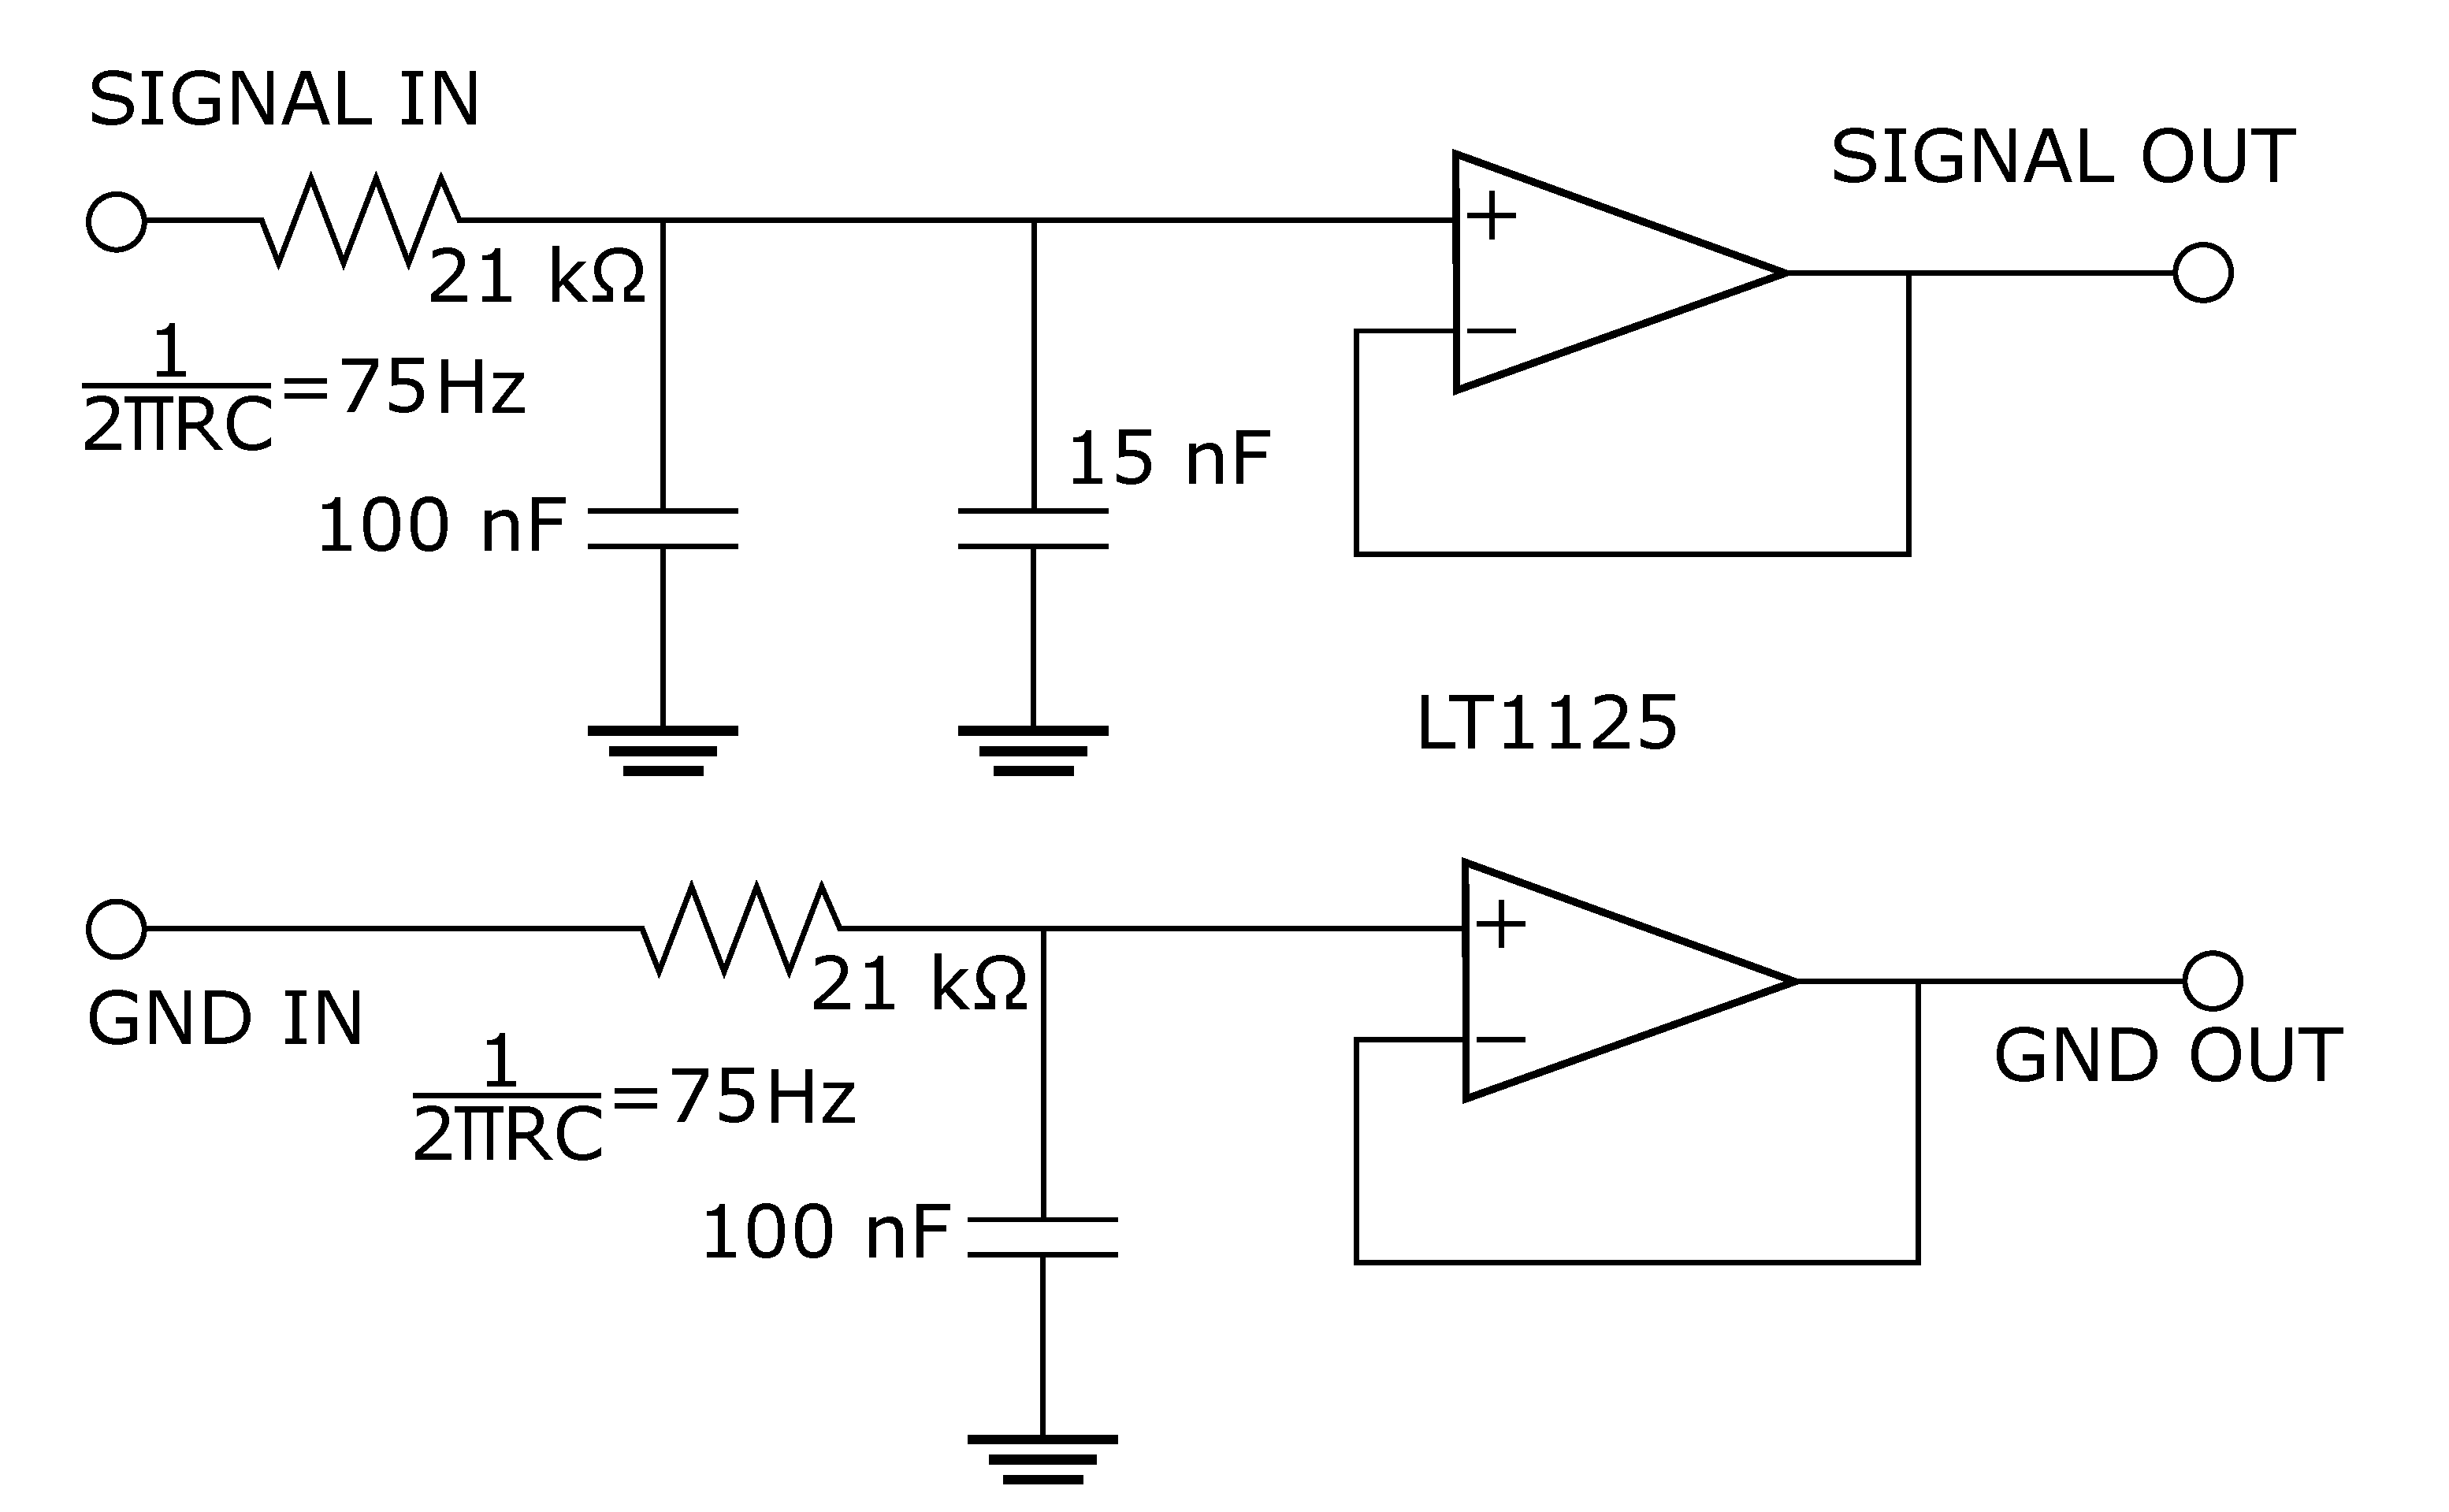
\includegraphics[scale=0.15]{Figures/DAQ_Filter.pdf}
\end{center}
\caption[Analog filter circuit]{\narrower A diagram of the circuit used to 
filter the output of the amplifier channel. Each photodiode signal is measured 
differentially, with 75 Hz lowpass filters on both the ground and signal 
inputs.}
\label{DAQ_Filter}
\end{figure}

The signal from each photodiode is measured using one of eight channels on a NI-USB-6281 data acquisition board. Before the signals are digitized, both the ground and the central conductor input are passed through one of 16 active filters to suppress noise and signal harmonics. The filter rolloff frequency of each filter, which is $(75 \pm 1)$ Hz. Although the phase shift at 8 Hz is small, the capacitors were measured and chosen carefully to match the time constant for all 16 filters. 

\chapter{Mercury Vapor Cells: Black magic in action}
\label{CellChap}
The importance of the vapor cells to the continuing success of the Hg EDM experiment cannot possibly be overstated. Far from being simple containers, these cells form the very heart of the apparatus, and all the time and effort which has gone into improving them has paid off many times over. Unfortunately, despite the effort and the number of high-quality cells that have been produced, very little has been attained in the way of a rigorous understanding of how these cells work. This relatively informal chapter is intended to serve as an exploration of the many different factors that go into making a good vapor cell, as well as a repository of accumulated ``lore'' that represents the current state of the art in making these highly specialized instruments. 

\section{Materials and fabrication}
The cell bodies were fabricated from 1-inch outer-diameter tubing of Heraeus suprasil fused silica, a chemically-refined powder of SiO$_2$ which is purified to remove defects including alkali metals and other contaminants before being fused into an inhomogeneous solid by means of an electrical arc or flame heating process. Two small-diameter (I.D. $\approx$ 1mm) suprasil tubes (referred to as ``stems'' in this work) were welded opposite each other and perpendicular to the axis of the central tubing. The large tubing was then cut into 10 mm segments with each pair of stems in the center. Such segments of tubing with stems attached are referred to as cell ``bodies''. To complete the assembly, two 1.5" diameter, 1/16" thick suprasil disks (``endcaps'') were coated with a thin film of tin (IV) oxide (SnO$_2$, also referred to as stannic oxide) and bonded to the top and bottom of each cell body. 

\begin{figure}
\begin{center}
\includegraphics[scale=0.8]{Figures/Cell_Picture.jpg}
\end{center}
\caption[A typical Hg vapor cell]%
{\narrower A typical Hg vapor cell, with wax visible in the cell stems and around the joint where the endcaps meet the cell body. When installed in the apparatus, laser beams enter and exit the cell body perpendicular to the stem axis.}
\label{HgCell}
\end{figure} 

\subsection{Glass preparation and assembly}
Prior to assembly, the endcaps and cell bodies were lapped flat and highly polished to minimize the gap between them, which typically varied by much less than one wavelength of visible light, as observed by the absence of a Newton interference fringe pattern around the rim when the endcap is placed on top of the cell body. The application of the SnO$_2$ coating did not impair the observed flatness of the endcaps against the cell bodies. A small chamfer was ground on the inner rim of each cell body to allow adhesive to be wicked around the joint between the body and endcap.  Before the endcaps were attached, adsorbed impurities were extracted from the glass pieces by placing them in a Soxhelet extractor with a 6 N solution of hydrochloric acid. The pieces were then rinsed in de-ionized water and air dried.

Once prepared, the endcaps were bonded to the cell bodies using KL-5 vacuum leak sealant, a mixture of silicone resin sold by the Kurt J. Lesker company as a general-purpose vacuum system leak solution. According to the manufacturer's specifications, the sealant is low-outgassing at temperatures up to 400 $^{\circ}$C. After the endcap was fitted against the cell body, a partial vacuum was maintained by fitting one end of a small rubber hose over the open cell stem and affixing a syringe on the other end. The syringe plunger was pulled back and the leak sealant was applied in a thin bead around the outer circumference of the cell body, after which it was allowed to wick inwards and cure for several days. Once joined, no excess adhesive is visible between the cell bodies and endcaps. After the assembly of the cells was completed, one stem of each cell was welded shut on the outside end, and the open stem was fused to a quartz vacuum manifold. 

\subsection{Filling and vacuum system work}
Six cells were attached to the vacuum system at a time, after which the system was pumped out and the glass sections baked to 50 $^{\circ}$C for 24 hours, followed by a second 24-hour bake to 180 $^{\circ}$C.\footnote{Prior to attaching the vapor cells to the quartz vacuum manifold, the glass sections of the vacuum system were baked to 325 $^{\circ}$C for several days.} After the cells were fitted to the vacuum system, the stems were heated to the annealing point (1150 $^{\circ}$C) for 20 s each to remove any adsorbed gases in the area, and the glass manifold was baked a third time to 160 $^{\circ}$C. A system base pressure of $5\cdot10^{-7}$ Torr was observed using an ion-gauge attached to the system.

\begin{figure}
\begin{center}
\includegraphics[scale=0.2]{Figures/Cell_Filling.jpg}
\end{center}
\caption[Vapor cells on vacuum manifold]%
{\narrower Six Hg vapor cells are suspended by the vacuum manifold above a reservoir of LN$_2$. Direct application of LN$_2$ was used to condense the Hg inside the cells, visible as grey spots on the near endcaps.}
\label{HgFilling}
\end{figure}

Each cell was then filled with approximately 1 g of dotriacontane wax (C$_{32}$H$_{64}$) prepared in a fractionating column to remove any dissolved gases and shorter carbon-chain molecules, as well as unsaturated alkanes and other impurities. Wax was distributed to each of the six cells from a separate break-seal ampule mounted to the vacuum system. To outgas contaminants, the wax was heated inside of its ampule while sealed off from the main chamber and vacuum pumps; some outgassing of the glass open to the vacuum system was also observed. The small U-tube between the break-seal ampule and the cell manifold was placed under liquid nitrogen (LN$_2$), forming a 'cold trap' to remove any condensible gases (CO$_2$, CH$_4$, H$_2$O, etc.) before they entered the cell manifold. A magnetic armature was used to break open the ampule by lifting it with a magnet from outside the glass vacuum system and dropping it (sometimes repeatedly) on the thin glass wall of the break-seal. Once the break-seal ampule with wax inside was open to the vacuum, the wax was evaporated with a blowtorch and re-condensed inside the main vacuum system. Then it was moved into the vapor cells using surface tension, by holding a hot soldering iron near the wax, thus ``pushing'' it away from the heat source.

Approximately 0.5 mg of isotopically-enriched $^{199}$Hg was condensed inside of each cell from a second break-seal ampule previously attached to the vacuum system. After the Hg was open to the rest of the vacuum system, it was condensed inside of the vapor cells by cooling the cell endcaps by application of liquid nitrogen for several hours. Once the Hg inside the break-seal had disappeared and could not be condensed on other parts of the vacuum system walls, it was assumed that all the available Hg had been consumed by the vapor cells. 

After filling with Hg, the wax was driven away from the cell entrance stem as well as possible using a soldering iron. The cold traps were then placed under liquid N$_2$, and 425 Torr of CO buffer gas was admitted into the system from a tank connected to an oxygen trap. The CO tank was connected to the manifold on the opposite side of the cold traps from the cells, so that condensible gases (CO$_2$, H$_2$O, etc.) would be frozen to the walls of the manifold before entering the cells. Each cell was then sealed off using an oxygen-propane torch, with the area of the stem near the flame carefully wrapped in wet paper towels to avoid cracking any remaining wax left near the entrance. Once sealed off, the wax was distributed around the inner surface of each cell by warming the glass with a hot air gun and moving the liquid wax under gravity. Once a thin coating was achieved, excess wax was moved towards the cell stems by holding the warm cell by the opposite stem and shaking the cell in an arc to drive the liquid wax to the stem and the outer rim. 
 
\section{Performance}
Perhaps the most marked difference between the latest generations of Hg vapor cells and previous sets is the behavior of the cells under heat and UV light exposure. Prior generations of cells would typically have characteristic spin-coherence times of $\approx$ 150s, which would decay under prolonged exposure to the UV pump and probe beams necessary for the experiment. It was found that by periodically removing the cells from the apparatus and re-melting the wax inside using a small flame torch, the coherence time could be temporarily extended, at the cost of a smaller Hg vapor density inside the cell \cite{Swallows}\cite{Griffith}. Of course, the loss of Hg placed an upper limit on the working life of a vapor cell, as the Hg precession signal would become smaller after each re-melting. The newest generations of cells exhibit radically different behavior under UV radiation, as their coherence time often increases after exposure to 254 nm light resonant with the Hg transition frequency. As such, these cells require no re-melting procedure and will theoretically remain functional after an indefinite amount of use. 

At present, the best explanation for the different behavior of new cells compared to old ones lies in the adhesive used to bond the endcaps to the cell bodies. Previous generations of Hg cells used Norland optical adhesive, an epoxy which is cured under UV light. This adhesive was found to contain sulfur compounds, which may react readily with Hg atoms. When cells from old batches were baked to 150 $^{\circ}$C, and then placed in a spectrophotometer, they were found to be completely opaque to UV wavelengths. This suggests that the sulfur may have outgassed from the epoxy and reacted with Hg atoms when the cells were heated. Mercury atoms were thus removed from the vapor phase, decreasing the signal size with each re-melting. The low-outgassing performance of the KL-5 vacuum leak sealant seems to have prevented this phenomenon with the new vapor cells.

\section{Surface coatings}
Some of the pioneering work on atomic vapor cells was done by Bouchiat and Brossel in the 1960s using isotopically-enriched atomic rubidium \cite{1966_Bouchiat_Brossel_Rb_relaxation}. From their studies, they concluded that short-range dipole-dipole interactions between the atoms and the cell wall are responsible for decoherence, and the effect of a wax coating on the cell wall is to reduce the ``sticking time'' during which a polarized atom near the wall will interact with the short-range magnetic fields generated by the spin distribution of the wall or coating. Working on previous generations of Hg EDM cells, Romalis and Lin also identified the predominant Hg spin relaxation mechanism as ``dipolar coupling to paramagnetic sites on the surface'' \cite{2004_Romalis_Lin_Hg_relaxation}. Their conclusions were motivated by the observed dependence of the coherence time on temperature and magnetic field strength inside the cell.

The effect of dipole interactions is generally larger in Rb than Hg because the magnetic dipole moment of a (ground state) Hg atom is the same as that of the nucleus (for isotopes with $\mathbf{I} \neq 0$), while the magnetic dipole of the Rb atom is primarily due to the unpaired electron. While the enhanced effect of dipole interactions typically leads to smaller attainable coherence times in Rb vapor cells than Hg cells, recent progress has been made with alpha-olefin coatings \cite{2010_Budker_long_Rb_coherence_alpha_olefins} which yielded Rb polarization times similar to Hg vapor cells without buffer gas \cite{2013_PSI_Hg_antirelaxation_coatings}. In contrast with the saturated (C$_{N}$H$_{2N+2}$) dotriacontane wax (with $N=32$) which is normally used for Hg cells, the olefins (also called alkenes) are unsaturated hydrocarbons with at least one carbon-carbon double bond. The alpha olefins (C$_{N}$H$_{2N}$) have one and only one such bond, located on one end of the hydrocarbon chain. 

To examine whether Hg cells with buffer gas might also be improved with coatings of unsaturated hydrocarbons, a set of four pre-fabricated quartz cells purchased from Starna Scientific were coated with the same alpha-olefins of varying length used in \cite{2010_Budker_long_Rb_coherence_alpha_olefins} and filled with CO buffer gas and a small amount of natural Hg. Intended for use in spectrophotometers, the cells used for this test had no tin (IV) oxide-coated surfaces or glued joints. Unfortunately, these cells did not appear to benefit from the different coating alone, as results for the coherence lifetime were less than 100 s. However, the olefins used were not refluxed to remove impurities (as the dotriacontane was), and the glass used in making the cells was also not identical to the suprasil used in the best $^{199}$Hg cells. These dissimilarities between the dotriacontane cells and the olefin cells imply that unsaturated coatings may deserve a more rigorous examination in the future.

\section{Excess Hg and polarization lifetime}
While any attempt at making high-quality vapor cells must involve careful attention to the preparation of wax or other surface coatings, Bouchiat and Brossel \cite{1966_Bouchiat_Brossel_Rb_relaxation} identified another important phenomenon which could compromise the quality of a vapor cell:

\begin{quote} A second class of difficulties exist, which have to do with surface physics: the making of coatings with properties which are reproducible from day to day or in different cells. The behavior of these coatings has been described elsewhere. We will recall briefly, later on, some of their properties, and we will stress the precautions one has to take in making them. \textit{Let us just say here that contamination by a Rb metal film must be avoided at all costs} [emphasis added].\end{quote} 
\begin{figure}
\begin{center}
\includegraphics[scale=0.8]{Figures/Hg_droplet_photo.jpg}
\end{center}
\caption[Interior surface of a cell endcap with $^{199}$Hg droplets]%
{\narrower A photo showing the interior surface of a Hg cell under a microscope at 100x magnification. Dark-colored spots are droplets of liquid Hg, which can be evaporated by contacting the exterior surface of the glass with a hot soldering iron. The black line is a feature of the particular microscope objective to be used for illustrative purposes.}
\label{HgDroplet}
\end{figure}
The mechanism behind the polarization-destroying properties of liquid metal films is obvious: If polarized Hg or Rb vapor exists in a cell in equilibrium with unpolarized metal in a film on the wall, then the film will exchange unpolarized atoms for polarized ones, leading to a maximum polarization decay time proportional to the fractional area of the wall covered by the film times the frequency of wall collisions for the typical atom. Our Hg vapor cells have a diffusion time $\approx$ 1 s and a surface area $\approx$ 18 cm$^2$, so to achieve a polarization time $>$ 250 s, the area of the wall covered by a thin film of Hg must be no larger than $\approx$ 7 mm$^2$. In principle, this appears to be a modest requirement, since the surface tension of liquid Hg is considerable, and the amount inside of each cell is quite small. However, it is difficult to know the exact distribution of liquid Hg in practice, since the interaction of thin films with the wax is not well understood, and any film covering a substantial area would only need to be atoms thick, thus rendering it all but invisible.

\begin{figure}
\begin{center}
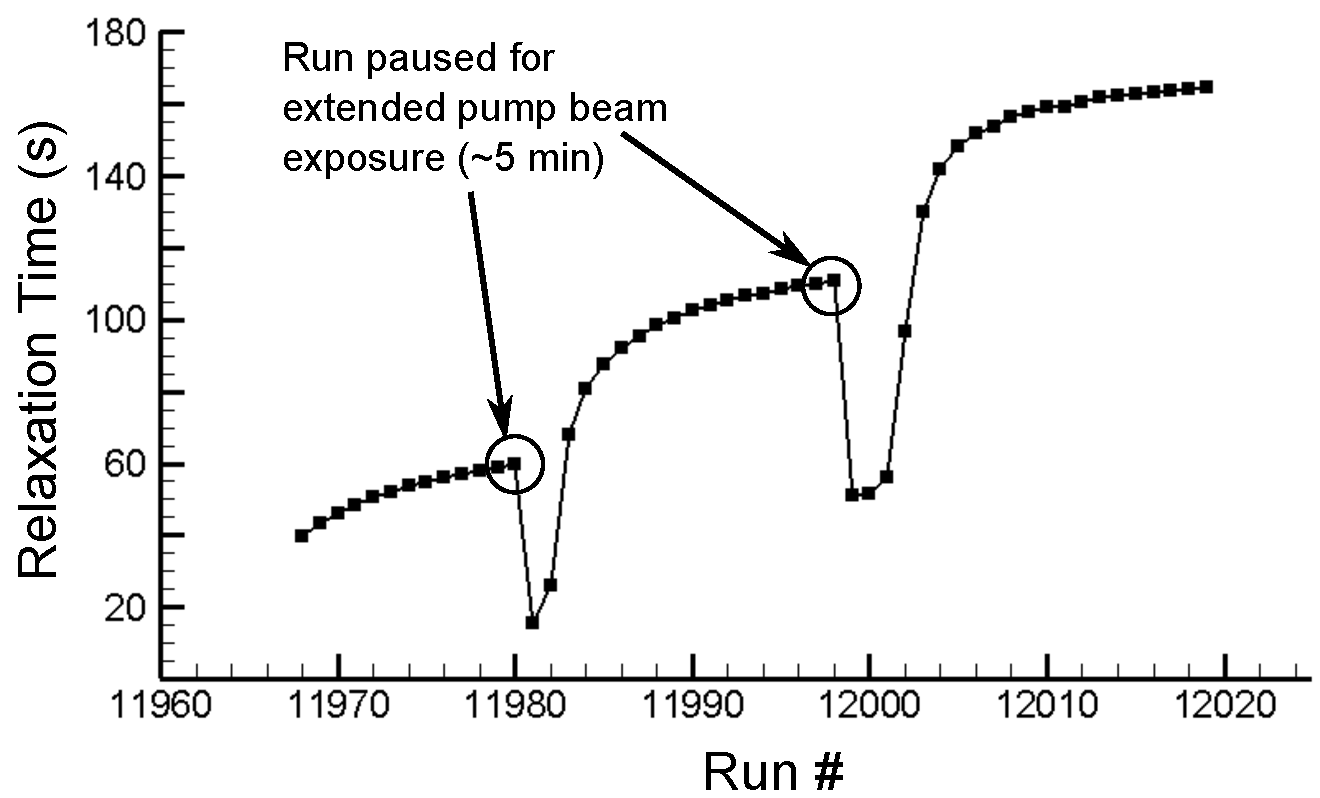
\includegraphics[scale=0.6]{Figures/Lifetime_UV_exposure.pdf}
\end{center}
\caption[Coherence time of a Hg cell with repeated resonant UV exposure]%
{\narrower Plot of atomic coherence time for an EDM cell with repeated prolonged exposure to the pump beam. Lifetimes increase with repeated pump/probe cycles, and the process can be accelerated by pausing the series of measurements to remove the cell and expose it to the undivided and unattenuated beam for several minutes at a time. Increases in lifetime are observed only when the beam is maintained at the resonant (pump) frequency. The increased rate of Hg nucleation with resonant light observed in \cite{1998_HgPhotonucleation} suggests that the improvement in coherence times is caused by UV-light-induced Hg redistribution.}
\label{LifetimeUV}
\end{figure}

\section{Resonant UV as droplet catalyst} \label{HgNucleation}
The possibility of thin films of liquid Hg on the cell walls also offers a potential explanation for the change in coherence time with resonant UV light exposure. Uchtmann \textit{et al.} report that the rate of droplet nucleation in supersaturated Hg vapor increases dramatically when the gas is illuminated with resonant light \cite{1998_HgPhotonucleation}. If exposure to resonant 254 nm light causes Hg to be deposited on the waxed cell surface in small droplets instead of a thin film, then the exposed surface area of unpolarized liquid Hg will decrease with exposure to light at the pump frequency. Figure \ref{HgDroplet} illustrates a view of the Hg droplets seen under magnification on the interior surface of a cell. 

It was found that these droplets can be easily formed into an aerosol by applying heat to the glass (typically using a hot soldering iron) and subsequently observed by the scattering of visible light output from a helium-neon (HeNe) laser. After suspending the droplets in the CO, exposure to an intense Hg UV lamp removes them from the vapor. The authors of \cite{1998_HgPhotonucleation} note that the ionization potential of a Hg droplet varies slowly from 10.4 eV (the ionization energy of a single Hg atom) to 4.7 eV (the work function of liquid Hg) with increasing size, beginning at a cluster size of only 13 atoms \cite{1991_Hg_Ionization_Potential}. These liquid droplets could thus be undergoing ion-induced nucleation, where a UV photon creates a photoelectron in a given droplet, which then polarizes and attracts uncharged droplets nearby. 

Given the behavior of the new cells to UV exposure, a course of cell conditioning was adopted that involved heating the cell gently to increase the Hg vapor density, and exposing it to the resonant pump beam to increase the lifetime. Figure \ref{LifetimeUV} illustrates the effect of repeated exposure to the UV beam on resonance after heating. Beginning at just 40 s, the coherence time of the cell increases slightly with normal pump-probe cycling, and eventually levels off. Once the increase between each measurement becomes small, the cell is removed from the apparatus and exposed to the full beam (with no attenuation, chopper wheel or beamsplitters) tuned to the pump frequency for approximately 5 minutes. After the prolonged exposure, the coherence lifetime dropped from the previous plateau before rapidly rising to a new, higher maximum.

The vapor cells that were used in the latest EDM publication exhibited a substantial reduction in coherence lifetime when they went unused for a period of several months. At the end of the data set, these cells had lifetimes in excess of 300-500 s, but after the apparatus was re-assembled with an additional layer of mu-metal shielding, the same cells had lifetimes of 50 s or less. Under normal pump-probe cycling, the lifetimes slowly began to improve, suggesting that the resonant laser light perturbs the distribution of Hg on the cell surfaces away from an equilibrium state which may take weeks or months to re-establish itself.

Finally, circumstantial evidence also suggests that increasing the quantity of Hg inside a a cell may improve the maximum achievable lifetime. Prior to making the cells with enriched $^{199}$Hg, a pair of cells were fabricated using natural Hg. While these cells were not suitable for the EDM experiment due to their reduced optical rotation amplitude, one of these test cells exhibited coherence times in excess of 1000 s, greater than that of any enriched $^{199}$Hg cell.\footnote{The other natural Hg cell had a more typical maximum lifetime near 500 s.} This cell also had a larger quantity of Hg, with a single drop inside easily visible to the naked eye. If all the atoms in the liquid phase are available to exchange with polarized atoms in the vapor phase (as opposed to being sealed inside the wax), then the lifetime will be maximized when the total liquid Hg surface area is at a minimum. The minimum surface area enclosing any given volume is a sphere, so the liquid Hg atoms will exert the minimum depolarizing effect if they are concentrated into a single spherical drop. If the large drop of liquid Hg acts as a sink for other Hg atoms on the surface, the liquid Hg inside may be more likely to agglomerate into a single, nearly-spherical drop, thereby minimizing the rate of exchange depolarization.

\chapter{Data Analysis}
\section{Data filtering}
\label{Digital_filter}
To begin the analysis, model the signal from each photodiode as 
\begin{align}
I_s(t) = I_0(t) \sin^2(\pi/4 + Ae^{-t/\tau}\sin(\omega t + \phi_0)) \\
I_p(t) = I_0(t) \cos^2(\pi/4 + Ae^{-t/\tau}\sin(\omega t + \phi_0)) 
\end{align}
where $I_s$ and $I_p$ represent the two linear polarization states of light from a given cell. $\pi/4$ is the equilibrium angle between the incident light and the polarizer axis, set by rotating a $\lambda/2$ waveplate located in front of the Wollaston prisms. Denoting the instantaneous angle between the light polarization and the polarizer axis as $\theta(t)$, the precession signal $S(t)$ for a given cell is obtained by subtracting the two polarization states from each other and dividing by the sum:
\begin{equation}
S(t) = \frac{I_s(t)-I_p(t)}{I_s(t)+I_p(t)} = \sin{2\theta} = \sin\lbrace 2\theta_0 \sin(\omega t + \phi) e^{-t/\tau}\rbrace. 
\end{equation}
Note that normalizing the difference in the two photodiode signals by the sum removes any time-dependent intensity fluctuations $I(t)$. After taking the normalized difference, each cell signal is sent to a simple digital filter to remove higher harmonics of the central frequency ($\approx$ 8.33Hz). The filter is based around averaging signal samples separated by time equal to $\pi/n\omega$, where $n\omega$ is the nth harmonic of the central frequency.

To begin building the harmonic filter, consider a signal $S(t_n)$ sampled at regular intervals $t_n$ with the functional form
\begin{equation} \label{S}
S(t_n) = A \sin(\omega t_n) + B \sin(2\omega t_n) + C \sin(3\omega t_n) + D. 
\end{equation}
As a rudimentary way to filter out the $2\omega$ component while preserving the fundamental frequency, we can simply average points separated by a time difference equivalent to a phase shift of $\pi$ at the undesired frequency. For the case of $2\omega$, this time shift is $\Delta t = \dfrac{\pi}{2\omega}$: 
\begin{equation}
S'(t_n) = S(t_n + \pi/4\omega) + S(t_n - \pi/4\omega)
\end{equation}
where $\sin(2\omega (t_n + \pi/4\omega)) = \sin(2\omega t_n + \pi/2) = - \sin(2\omega t_n - \pi/2).$ The precession frequency of the EDM cells is tuned by changing the average magnetic field $B_0$ so that the sampling frequency (200 Hz) is 24 times the Larmor frequency. The phase of each signal can thus be easily shifted by $\pi/n $ (for $n=2,3,4$) by moving an integer number of steps through the data stream.

For the $1\omega$, $2\omega$, and $3\omega$ frequency components of the signal, the time shift $t_n \rightarrow \pm t_n + \pi/4\omega$ creates phase shifts of $\pi/4$, $2\pi/4$, and $3\pi/4$, respectively. The frequency components transform according to
\begin{align}
A\sin(\omega t_n) & \rightarrow A[\sin(\omega t_n + \pi/4) + \sin(\omega t_n - \pi/4)] = \sqrt{2}A \sin(\omega t_n) \\
B\sin(2\omega t_n)& \rightarrow B[\sin(\omega t_n + 2\pi/4)+ \sin(\omega t_n - 2\pi/4)]= 0\\
C\sin(3\omega t_n)& \rightarrow C[\sin(\omega t_n + 3\pi/4)+ \sin(\omega t_n - 3\pi/4)]= -\sqrt{2}C\sin(3\omega t_n)
\end{align} 
removing the $2\omega$ component and retaining the fundamental frequency component as well as the $3\omega$. We can remove the $3\omega$ term and the constant offset $D$ by performing a second, similar procedure on the filtered array $S'(t_n)$: 
\begin{equation}
S''(t_n) = S'(t_n + \pi/3\omega) - S'(t_n - \pi/3\omega)
\end{equation}
where the subtraction removes the static contribution, and the $\pm\pi$ phase shifts for a $3\omega$ term amount to a sign change which sends the difference to 0. For the fundamental frequency component, we are left with
\begin{equation}
\sqrt{2} A \sin\omega t_n \rightarrow \sqrt{2} A [\sin(\omega t_n + \pi/3) + \sin(\omega t_n - \pi/3)] = \sqrt{6} A \cos\omega t_n 
\end{equation}
Combining the two filters into a single expression, we have
\begin{equation}
S''(t_n) = S(t_n + \dfrac{7\pi}{12\omega}) + S(t_n + \dfrac{\pi}{12\omega}) - S(t_n - \dfrac{\pi}{12\omega}) - S(t_n - \dfrac{7\pi}{12\omega}).
\end{equation}
Because the Larmor frequency $\omega$ is set at 24 times the sampling frequency of the experiment, $\Delta t = t_{n+1} - t_n = \pi/12\omega.$ Then we can express the filter function in terms of the nth sample:
\begin{equation}
S''(t_n) = S(t_{n+7}) + S(t_{n+1}) - S(t_{n-1}) - S(t_{n-7}).
\end{equation}

However, the adjustment of the Larmor frequency to be an integer multiple of the sampling frequency is not perfect. If we parameterize the timing error by $\pi/12\omega = \Delta t + \epsilon,$ we can calculate the correction needed for the digital filter by substituting (\ref{S}) into our expression for $S''(t_n)$ above:
\begin{align} \label{filter_error}
S''(t) = & 2A\cos \omega t \left[\dfrac{\sqrt{3}+1}{2\sqrt{2}}\cos 7\omega\epsilon + \dfrac{\sqrt{3}-1}{2\sqrt{2}}\cos \omega\epsilon - \dfrac{\sqrt{3}+1}{2\sqrt{2}} \sin\omega\epsilon + \dfrac{\sqrt{3}-1}{2\sqrt{2}}\sin 7\omega\epsilon\right] \\ 
+ & 2B\cos 2\omega t\left[\dfrac{-1}{2}\cos14\omega\epsilon + \dfrac{1}{2}\cos2\omega\epsilon + \dfrac{\sqrt{3}}{2}\sin 14\omega\epsilon - \dfrac{\sqrt{3}}{2}\sin 2\omega\epsilon\right] \\ 
+ & 2C\cos3\omega t \left[\dfrac{-1}{\sqrt{2}}\cos21\omega\epsilon + \dfrac{1}{\sqrt{2}}\cos3\omega\epsilon - \dfrac{1}{\sqrt{2}}\sin21\omega\epsilon - \dfrac{1}{\sqrt{2}}\cos3\omega\epsilon \right]
\end{align}
Note that as $\epsilon \rightarrow 0$, $\cos(n\omega\epsilon) \rightarrow 1$ and $\sin(n\omega\epsilon) \rightarrow 0$. The term in (\ref{filter_error}) proportional to $\cos(\omega t)$ therefore reduces to $\sqrt{6}\cos(\omega t)$, and we can neglect the factor in braces. The remaining terms are calculated in the data analysis code and added as a correction to the filtered data arrays before being fit for a phase difference.

\section{Individual cell frequency fits}
After the harmonic filtering, the cell signals are monotonic sine waves with a central frequency in the neighborhood of 8.33Hz and a decaying exponential envelope function determined by the individual cell lifetime. The method used to fit each cell signal is a Leavenberg-Marquardt non-linear $\chi^2$ minimization routine based on the procedure in \cite{NumericalRecipes}[ch.15]. The details of individual cell frequency fits are described in detail in \cite{Griffith} and \cite{Swallows}, and our approach is extremely similar, to the point that details of the technique are not covered in this thesis. However, the cell signals in this work typically have larger amplitudes than in previous iterations of the experiment, so the fit function was modified to include the first non-linear correction term, proportional to $A^3$:
\begin{equation}
y(t) = \lbrace A e^{-t/\tau} + (A^3/6)e^{-3t/\tau} \rbrace \sin(\omega [t-t_0] + \phi)
\end{equation}
\textit{cf.} \cite[eq. 4.7]{Swallows}, \cite[eq. 4.4]{Griffith}.

\section{Phase difference measurements}
The exponential amplitude decay envelope is removed from each cell signal by applying a phase shift of $\pi/2$ to send the cell signals from $\sin\theta(t) \rightarrow \sin(\theta\pm \pi/2) = \pm \cos\theta$. This phase shift is applied by calculating a time shift $\Delta t = \pi/2\bar{\omega}$. The signals are digitized at a rate of 2kHz, then averaged and written to file at a rate of 200Hz, so the average precession frequency is tuned to make $\Delta t$ equal to 6 times the sampling period. Then, for a decaying sine wave sampled at times $t_n$, 
\begin{align}
 A^2e^{-2t/\tau} [\sin^2\theta(t_n)-\sin\theta(t_{n+6}) \sin\theta(t_{n-6})] \\ 
=A^2e^{-2t/\tau} [\sin^2\theta(t_n)-\sin(\theta(t_n) + \pi/2) \sin(\theta(t_n) - \pi/2)] \\
=A^2e^{-2t/\tau} [\sin^2\theta(t_n)-(\sin^2\theta(t_n) \cos^2\pi/2 - \cos^2\theta(t_n) \sin^2\pi/2)]\\
=A^2e^{-2t/\tau} [\sin^2\theta(t_n) + \cos^2\theta] \\
=A^2e^{-2t/\tau}
\end{align}
The decaying amplitude term is thus isolated and removed from each cell signal, leaving a sine wave of unit amplitude. The phase difference from each cell pair is extracted for each probe period by again phase-shifting the signal and using the trigonometric identity $\sin(\alpha-\beta) = \sin(\alpha)\cos(\beta)-\cos(\alpha)\sin(\beta)$
\begin{multline}
\sin(\omega_A t_n + \phi_A -\omega_B t_n - \phi_B) = \\ 
  \sin(\omega_A t_n + \phi_A) \sin(\omega_B t_{n-6} + \phi_B) 
- \sin(\omega_B t_n + \phi_B) \sin(\omega_A t_{n-6} + \phi_A)
\end{multline}
Computing the inverse sine of the above function gives a representation of the instantaneous phase difference between the cells as a function of time. The first derivative is the frequency difference between the cells, while the offset is equal to the initial or final phase difference, depending on which time $t_n$ is referenced to zero.\footnote{Because the frequency and phase differences between cells are small (angular frequency differences are typically of order $10^{-5}$, phase differences are typically $10^{-3}$ or less) we can approximate the signal by a straight line without the inverse sine function up to corrections on the phase difference of order $\theta^3\approx 10^{-9}.$ The change in the frequency difference for phase corrections of this size is two orders of magnitude smaller still, and therefore negligible.}

\section{Frequency difference from $\Delta\phi$}
Two separate methods are used to extract a measurement of the frequency difference in the dark from the two probe period data trains. The first method is to apply a simple least-squares fit to the A and B probe periods, modeling the data as a straight line with slope equal to the frequency difference and offset equal to the initial (or final) phase difference. Then the end point of the A period phase difference is compared to the initial B period phase difference, and the difference of the two is divided by the dark time $\Delta t_{Dark}$ for a \textit{Phase Fit} frequency difference $\Delta\omega_{PF} = \Delta\phi_{PF}/\Delta t_{Dark}$. 
\begin{figure}
\begin{center}
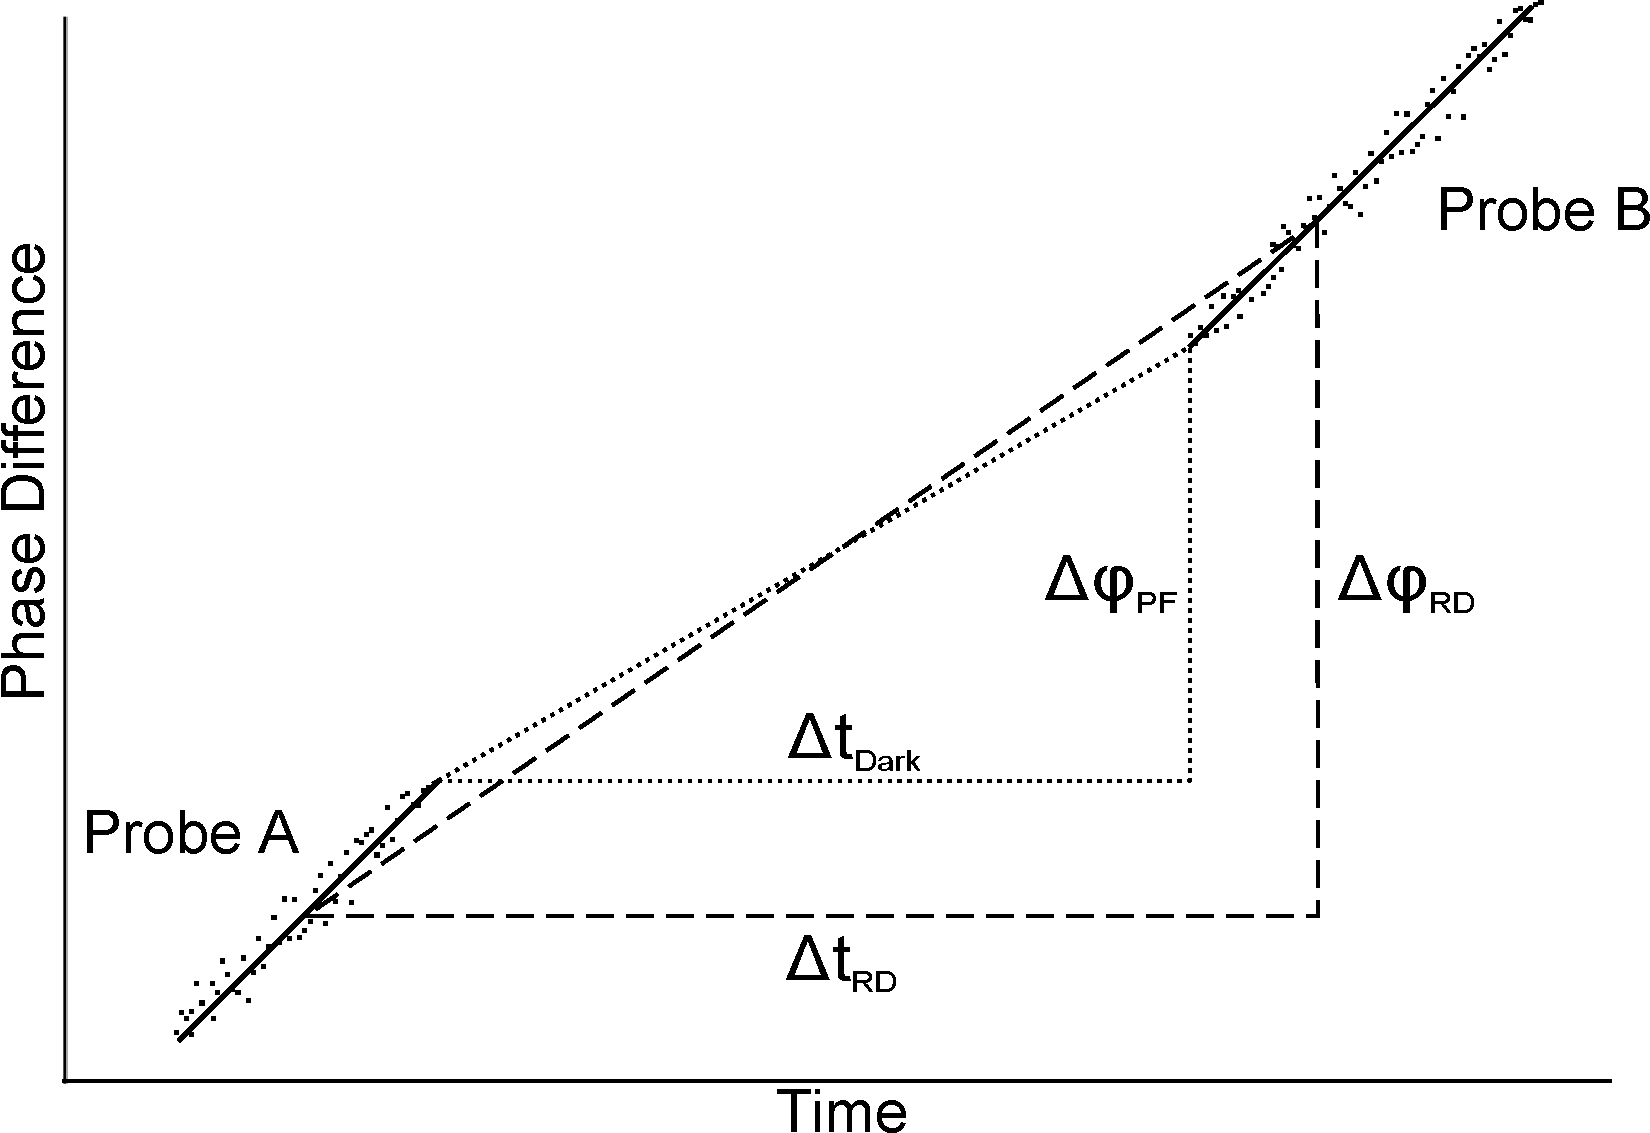
\includegraphics[scale=0.4]{Figures/Tdiff.pdf}
\end{center}
\caption[Comparative illustration of frequency difference methods]
{\narrower Diagram of the two primary methods of determining $\Delta\omega$ from $\Delta\phi (t)$. The first method fits the A and B periods to $\Delta\phi(t) = \Delta\omega \cdot t + \Delta\phi_0$, then finds the accumulated phase difference in the dark $\Delta\phi_{PF}$ from the fit parameters. The second method simply subtracts the \textit{n}th raw data point in the A period from the corresponding point in the B period raw data and averages the set of differences for $\Delta\phi_{RD}$. A light-induced shift of the frequency difference causes the two methods to disagree, as indicated by the difference in slope between the diagonal dashed/dotted fit lines.}
\label{TDiffVsPhaseFit}
\end{figure}
The second method breaks the data set from a given scan into pairs of raw points, one drawn from the A period and the other from the B period. An independent measure of the frequency difference can then be obtained from each pair of points. Denoting the \textit{n}th data point in the A (B) period as $\Delta\phi^A_n$ ($\Delta\phi^B_n$), the \textit{Raw Difference} method (also referred to as the \textit{Tdiff} method) determines a frequency difference 
\begin{equation}
\Delta\omega = \dfrac{1}{N} \sum^N_{n=1} \dfrac{\Delta\phi^B_n - \Delta\phi^A_n}{\Delta t_{RD}}
\end{equation}
where $\Delta t_{RD}$ is equal to the dark time $\Delta t_{Dark}$ plus the length of the A probe period. The increased time difference $\Delta t_{RD} > \Delta t_{Dark}$ yields a fit with a smaller error bar (determined by the scatter in the set of raw phase difference values) than the corresponding uncertainty in the phase fit (determined by the derivative of $\chi^2$ with respect to the value of fit parameters).

\begin{table}[t]												
\begin{center} 															
\caption[Phase fit vs. raw difference results with fixed $\Delta\omega_{OT-OB}$ coefficient] 
{\narrower Comparison of the two primary frequency difference analysis methods on the EDM frequency channel $\Delta\omega_{EDM} = \Delta\omega_{MT-MB} - (1/3) \Delta\omega_{OT-OB}$.}
\label{PFitV}
\begin{tabular}{cccccc} 													
\hline \hline                												
HV & $\mathbf{B}_0$ & Runs & Phase fit ($10^{-10}$ s$^{-1}$) & Raw diff. ($10^{-10}$ s$^{-1}$) & Change ($10^{-10}$ s$^{-1}$) \\
\hline          
10.357 kV &  +  & 72 & $(1.315 \pm 2.718) $  &  $(-1.885 \pm 2.230)$  &  $(3.200  \pm 3.516)$ \\
10.357 kV &  -  & 58 & $(3.605 \pm 3.031) $  &  $(4.204  \pm 2.475)$  &  $(-0.598 \pm 3.913)$ \\
6.219 kV  &  +  & 62 & $(1.844 \pm 2.998) $  &  $(1.814  \pm 2.442)$  &  $(0.030  \pm 3.867)$ \\
6.219 kV  &  -  & 60 & $(3.972 \pm 2.929) $  &  $(5.064  \pm 2.421)$  &  $(-1.092 \pm 3.800)$ \\
\hline 																	
\end{tabular} 
\end{center}															
\end{table}

\begin{table}[t] 											
\begin{center} 															
\caption[Phase fit vs. raw difference results with variable $\Delta\omega_{OT-OB}$ coefficient] 
{\narrower Comparison of the two primary frequency difference analysis methods on the EDM frequency channel $\Delta\omega_{EDM} = \Delta\omega_{MT-MB} - k\Delta\omega_{OT-OB}$ with variable daily outer cell coefficient.}
\label{VPFitV}
\begin{tabular}{cccccc} 													
\hline \hline                												
HV & $\mathbf{B}_0$ & Runs & Phase fit ($10^{-10}$ s$^{-1}$) & Raw diff. ($10^{-10}$ s$^{-1}$) & Change ($10^{-10}$ s$^{-1}$) \\
\hline   
10.357 kV &  +  & 72 & $(1.196 \pm 2.578)$  &  $(-1.6327 \pm 2.122)$ &  $(2.828  \pm 3.340)$ \\
10.357 kV &  -  & 58 & $(3.240 \pm 2.878)$  &  $(3.7105  \pm 2.354)$ &  $(-0.470 \pm 3.718)$ \\
6.219  kV &  +  & 62 & $(2.280 \pm 2.863)$  &  $(2.3723  \pm 2.336)$ &  $(-0.092 \pm 3.696)$ \\
6.219  kV &  -  & 60 & $(5.288 \pm 2.787)$  &  $(5.9405  \pm 2.304)$ &  $(-0.653 \pm 3.616)$ \\
\hline 																	
\end{tabular} 
\end{center}													
\end{table}

However, the two methods will disagree with each other if the slope of the A and B period data trains does not equal the average dark frequency difference $\Delta\phi_{PF}/\Delta t_{Dark}$. Frequency shifts induced by the presence of the probe light can perturb the measured frequency difference from the average value in the dark. Because the raw difference method incorporates the A and B probe periods into the measurements, it is sensitive to these potential light shift systematics. We therefore take the averaged value of the phase fit method to be our final result for the EDM. A comparison of the results generated by the two methods is shown in Tables \ref{PFitV} and \ref{VPFitV}. 


\section{HV correlation}
During EDM data runs, the HV polarity is reversed between each pump-probe cycle, so the signature of an EDM is the correlation between $\Delta \omega$ and the difference in the electric field. In the absence of any noise sources, this so-called \textit{dipole} HV reversal pattern implies that the middle cell frequency difference $\Delta \omega_{MT-MB}$ would have an opposite sign for each successive measurement. Because data points are equally spaced in time, finding the correlation of the signal with the HV is equivalent to isolating the component of the signal which oscillates at the Nyquist frequency. The simplest high-pass filter method is to take the difference between successive points

\begin{figure}
\begin{center}
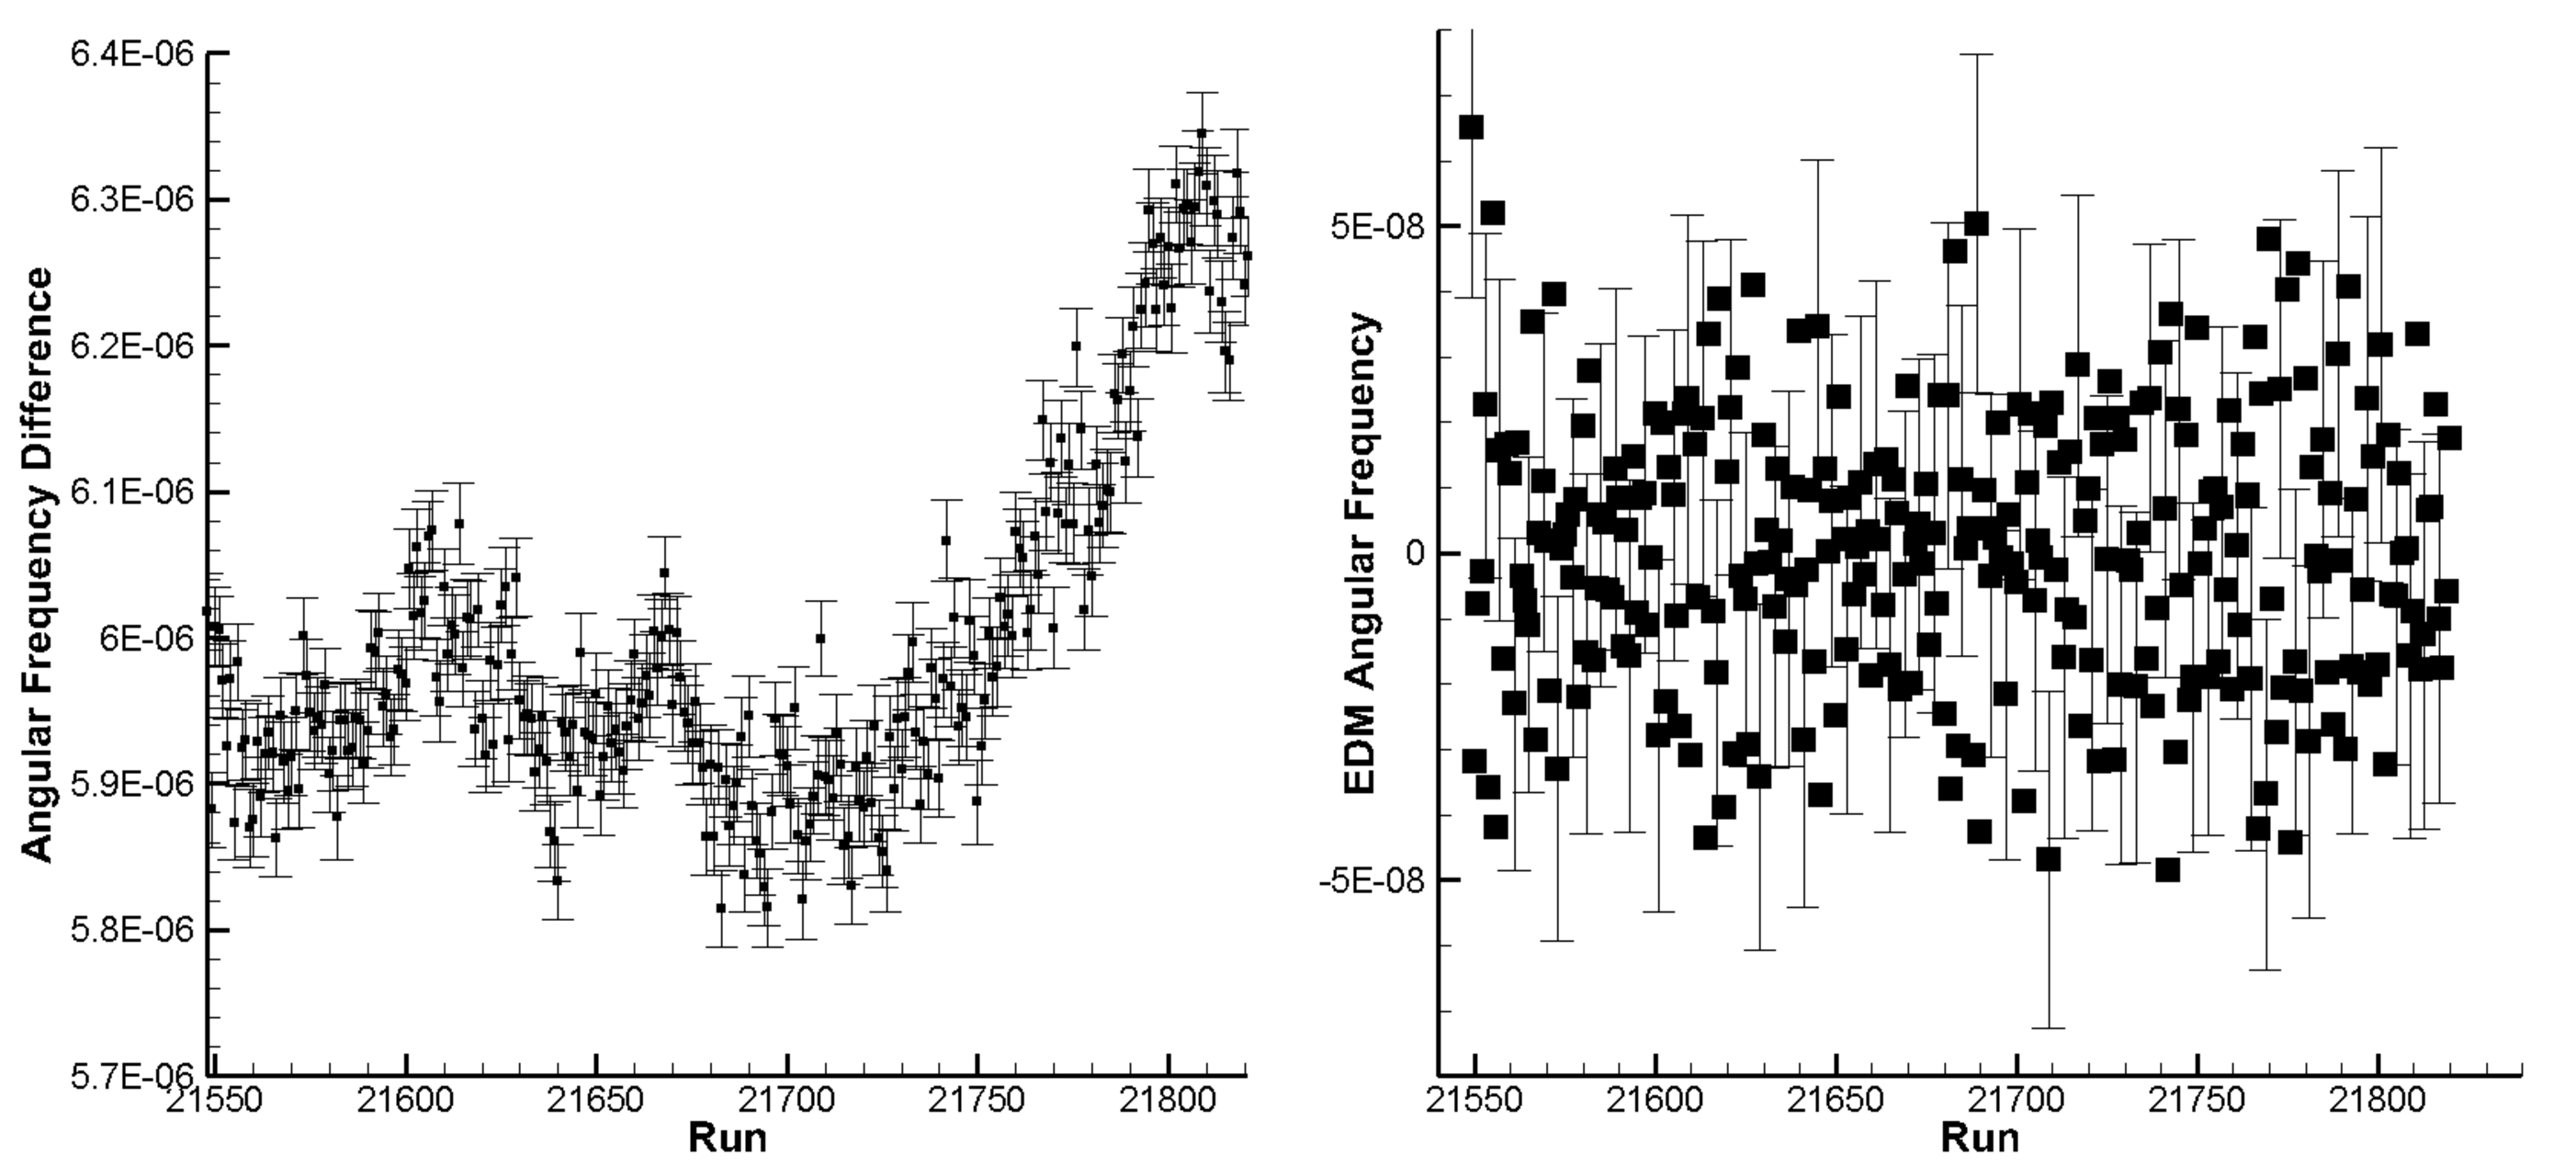
\includegraphics[scale=0.3]{Figures/SampleRun.pdf}
\end{center}
\caption[EDM frequency difference $\Delta\omega_{EDM}$ raw data]%
{\narrower Left: Individual raw points corresponding to the measured value of $\Delta\omega_{EDM}$ for successive pump-probe cycles. Note the large offset from zero due to the static third-order field gradients, and the slow drift with time. Right: The data after filtering with a simple 3-point high pass digital filter}
\label{SampleRun}
\end{figure}

In reality, $\Delta \omega_{MT-MB}$ is also sensitive to fluctuations in the gradients of $\mathbf{B}_0$. To reduce the impact of ambient magnetic field gradient noise, we use the outer cells as magnetometers and define our EDM signal as $\Delta \omega_{EDM} = \Delta \omega_{MT-MB}- (1/3)\Delta \omega_{OT-OB}$.

To reduce the impact of ambient magnetic field gradient noise, we use the outer cells as magnetometers and define our EDM signal as $\Delta \omega_{EDM} = \Delta \omega^D_{MT-MB}- k\Delta \omega^D_{OT-OB},$ where $k$ is the coefficient that minimizes the variance of the HV-correlated part of $\Delta \omega_{EDM}$ within each daily set of measurements. Runs with small values for $k$ reflect a low level of gradient noise (which is common to $\Delta \omega^D_{MT-MB}$ and $\Delta \omega^D_{OT-OB}$) relative to the statistical uncertainty in $\Delta \omega^D_{OT-OB}$, which simply adds noise to $\Delta \omega_{EDM}$ if $k > 0$ and gradient noise is absent. When gradient noise dominates, the value of $k$ goes to $1/3$ for maximum common-mode noise rejection. Throughout the data set, the value of $k$ varied from 0.18 to 0.33 with an average of 0.25.

\section{Shot noise limit}
The fundamental limitations on the EDM experiment performance derive from the finite number of photons used to make the measurement.\footnote{A similar noise limit can be calculated based on the number of atoms, but in practice the shot noise limit on the detected photons is much higher \cite{Swallows}.} The photodiode detectors used produce one electron of current for each detected photon, so we can obtain the photon shot noise limit by considering the photocurrent. The shot noise on the current can be derived simply from counting statistics: if, on average, N electrons worth of current arrive within a measurement time $\Delta t$, the standard deviation on the number counted in any given sample is $\sqrt{N}$, and the corresponding rms fluctuation on the current is $q\sqrt{N}/\Delta t$, where q is the charge. The voltage produced at the output of the transimpedance amplifiers follows $V=IR$, so the rms voltage fluctuations $\sigma_V$ obey the relation
\begin{equation}
\sigma_V = \sigma_I R = q R \sqrt{N}/\Delta t.
\end{equation}
Substituting for N, we have
\begin{equation}
\sigma_V = \dfrac{q R \sqrt{V\Delta t/qR}}{\Delta t} = \sqrt{\dfrac{VqR}{\Delta t}}.
\end{equation}
Because the shot noise is frequency independent (or white), the rms fluctuations diminish as $1/\sqrt{\Delta t}$. Dividing by bandwidth $B = 1/2\Delta t$, we get the noise amplitude per unit bandwidth
\begin{equation}
\sigma_V = \sqrt{2qVR}/\sqrt{\text{Hz}}.
\end{equation}
Using a typical value for an inner-cell photodiode intensity of 3.5 V and an impedance gain of $5 \cdot 10^{-7} \Omega$, together with an effective sampling frequency of 200 Hz,\footnote{Photodiode signals are digitized at 2 kHz, the average of each 10 sampled is recorded on file.} the shot noise limit on the voltage is $\approx 1.0 10^{-4}$ V. Similarly for the outer cells, a typical average photodiode intensity is 4.0 V across $1 \cdot 10^{-8} \Omega$, giving a shot noise limit of $\approx 1.6 \cdot 10^{-4}$ V. 

Monte Carlo simulations of the experiment using synthesized data trains with Gaussian-distributed noise added at the above levels returned an overnight (265 scans of 240 s each) EDM frequency error bar of $\Delta \omega_{EDM} = 1.44 \cdot 10^{-9}$ s$^{-1}$. Typical error bars for daily runs range from 2.0 to 3.0 $\cdot 10^{-9}$ s$^{-1}$, suggesting that we are a factor of 2 over photon shot noise.  However, the photon shot noise only enters into the calculation of $\Delta\phi$ for each probe period. For an arbitrarily long dark time $\Delta t$, a given statistical uncertainty in $\Delta\phi$ has no influence on $\Delta\omega = (\Delta\phi_B - \Delta\phi_A)/\Delta t$, so the shot noise is not a fundamental limit on the performance of the experiment.

\section{Blind data cuts}
To make data cuts without biasing the result, the frequency difference of each cell pair is added to a computer-generated blind offset during the HV correlation portion of the data analysis. For each probe period, the offset is applied to the phase difference $\Delta\phi$ of any pair of cells which has a non-zero $\mathbf{E}$-field difference (the only exception being $\Delta\omega_{OT-OB}$). The phase offset has opposite sign for probe periods $A$ and $B$, so the frequency difference is offset by twice the phase offset divided by the measurement dark time. The value of the phase offset is encoded within a binary file which is kept separate from the data analysis code to prevent inadvertent discovery when changes are made to the HV correlation analysis program. The value of the offset is proportional to the polarity and magnitude of the voltage across each cell, and the sign also changes with the direction of $\mathbf{B}_0$ to mimic the symmetry properties of an EDM. The magnitude of the offset per unit voltage was randomized with each new sequence to prevent introducing bias by ``herding'' the data--preferentially discarding runs far from the average value of the data already gathered.

The EDM data set is defined as the set of all dipole runs (with $+-+-$ HV pattern) which meet three criteria:
\begin{enumerate}
\item The run consists of at least 35 3-point strings (37 independent frequency scans)
\item The dipole scans are immediately followed by a set of quadrupole scans ($+0-0$ HV pattern)
\item The run is part of a sequence with at least 3 $\mathbf{B}_0$ reversals with 10 kV and 6 kV runs in between
\end{enumerate}
The cuts are made to enforce the assumption that when the apparatus is working properly, the EDM-insensitive frequency combinations should have no measurable HV correlation. The final cuts were made based on the two lowest-order symmetric and anti-symmetric frequency difference combinations, as follows: 
\begin{enumerate}
\item $|\Delta\omega_{OT-OB}| > 2.0 \sigma$ 
\item $|\Delta\omega_{OT-OB}| > 2.2 \cdot 10^{-8}$ s$^{-1}$
\item $|\Delta\omega_{Leak Test}| > 3.0 \sigma$ 
\item $|\Delta\omega_{Leak Test}| > 1.5 \cdot 10^{-8}$ s$^{-1}$ 
\end{enumerate}

Each channel is subject to two related cuts. Cuts \#1 and 3 remove runs which have a central value resolved by their own error bar $\sigma$, where $\sigma$ is determined by the standard deviation of the individual string points in the run. Cuts \#2 and 4 are intended to remove runs with relatively large error bars which may not be resolved, but which have central values more than 2.0 (3.0) standard deviations from the average of all 284 EDM runs on $\Delta\omega_{OT-OB}$ $(\Delta\omega_{Leak Test})$, where the standard deviation is computed from the set of runs. $\Delta\omega_{OT-OB}$ is sensitive to changes in a linear field gradient $\partial B_y/\partial y$, while $(\Delta\omega_{Leak Test})$ is equivalent to the difference between the average frequencies of the inner and outer cells and can indicate HV correlations in the second derivative $\partial^2B_y/\partial y^2.$ After the final cuts, our data set consists of 252 runs encompassing $\sim$65,000 frequency scans to be analyzed for an EDM. The effect of the data cuts on the EDM result is covered in detail in the discussion of systematic uncertainties in chapter \ref{SystematicChapter}.

\chapter{Statistical Fluctuations and Noise Sources}
\section{Statistical uncertainty}
\begin{figure}[t] \label{10kV_final_result_graph}
\begin{center}
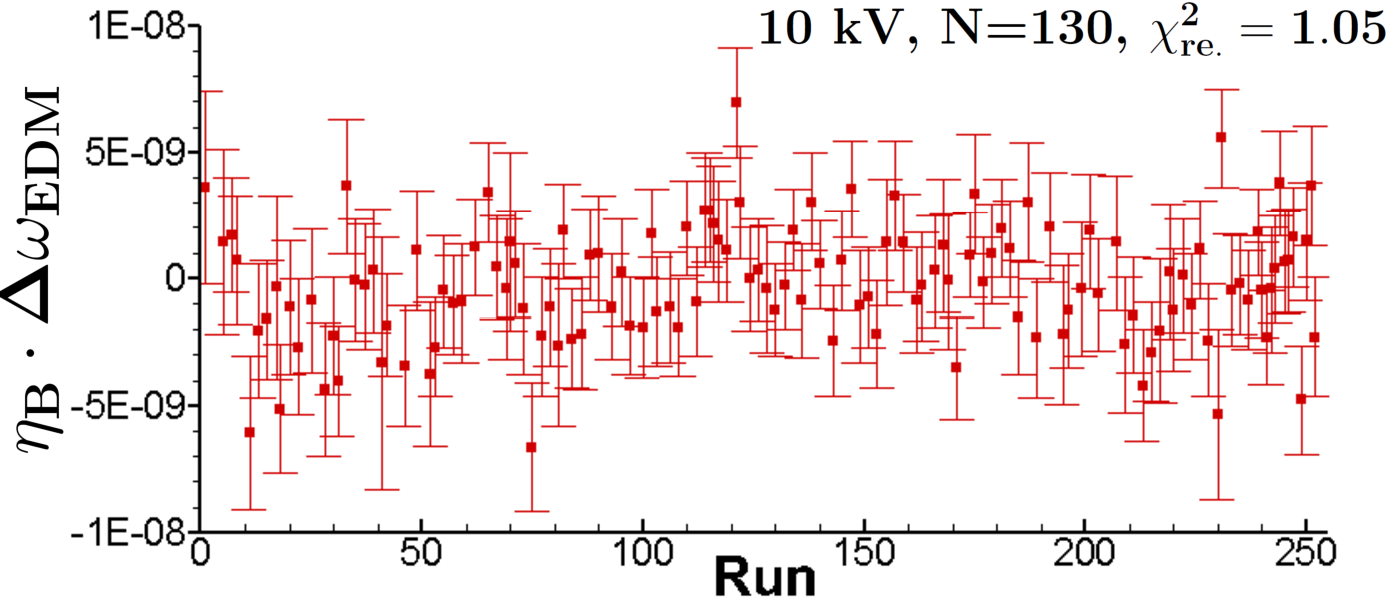
\includegraphics[scale=0.6]{Figures/10kV_Final_Datatset_Graph.pdf}
\end{center}
\caption[Final EDM data set, $\pm$10 kV runs]
{\narrower The measured EDM frequency shift $\eta_{\mathbf{B}}\cdot\Delta \omega_{EDM}$ for each of the 122 runs in the final data set measured between $\pm 10$ kV/cm. Error bars are obtained from the variance between individual frequency difference measurements within each daily run.}
\end{figure} 
The primary source of uncertainty in the EDM measurement is the statistical fluctuations in the measured value of $\Delta\omega$ for any pair of cells between one measurement and the next. Figures \ref{10kV_final_result_graph} and \ref{6kV_final_result_graph} show the 252 runs in the final dataset, broken out by the magnitude of the applied voltage. All data points represent the frequency shift measured from positive to negative applied voltage $\omega_{HV+} - \omega_{HV-}$. The central values of the runs in these graphs are multiplied by $\eta_{\mathbf{B}} = \pm 1$ depending on the projection of $\mathbf{B}_0$ onto the vertical axis. For runs with $\mathbf{B}_0$ directed up, $\eta_{\mathbf{B}} = 1$, and $\eta_{\mathbf{B}} = -1$ for runs with $\mathbf{B}_0$ directed down. With this sign change in place, a non-zero EDM value will manifest as a nonzero average value for the frequency shift. Because the frequency shift for a given EDM value is also linear in the applied $\mathbf{E}$ field, a non-zero frequency shift should also scale with the HV. 

\begin{figure}[t] \label{6kV_final_result_graph}
\begin{center}
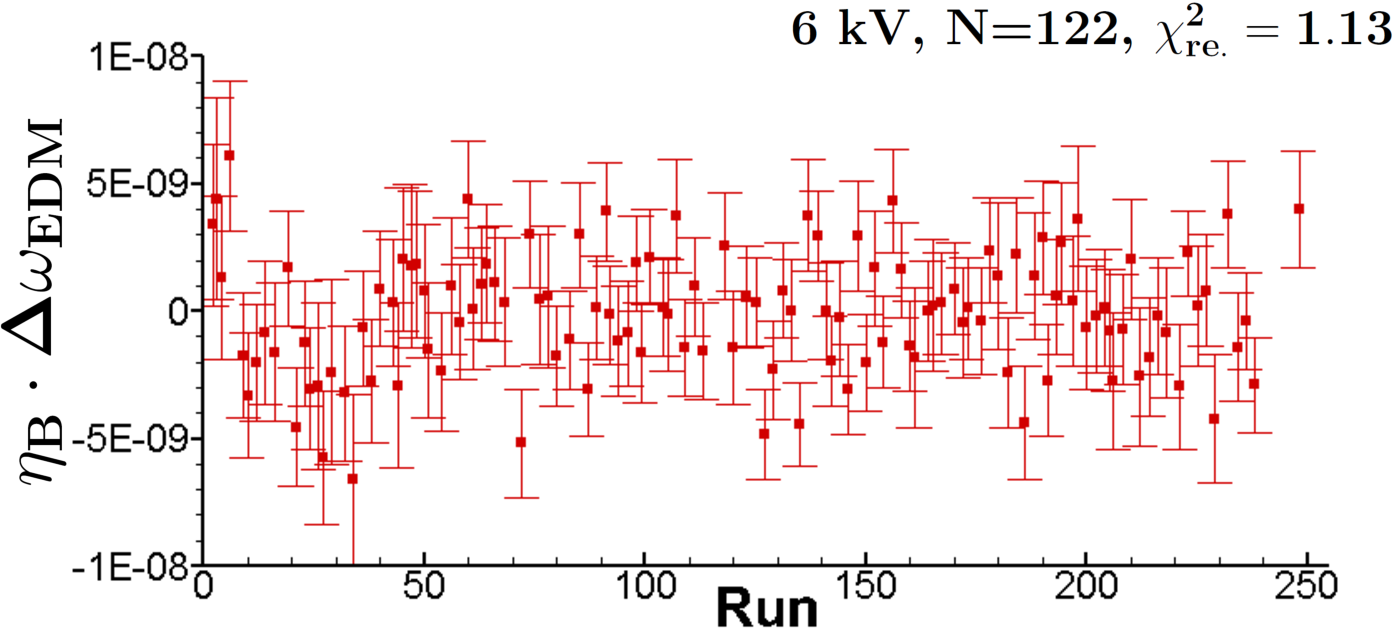
\includegraphics[scale=0.6]{Figures/6kV_Final_Datatset_Graph.pdf}
\end{center}
\caption[Final EDM data set, $\pm$6 kV runs]
{\narrower The measured EDM frequency shift $\eta_{\mathbf{B}}\cdot\Delta \omega_{EDM}$ for each of the 122 runs in the final data set measured between $\pm 6$ kV/cm.}
\end{figure}

\begin{table} \label{final_result_table}															
\begin{center}
\caption[Measured frequency shifts by field configuration]
{\narrower Measured HV-correlated frequency shifts for various field configurations. Entries for $\Delta\omega$ are specified in units of $10^{-11}$ (kV$\cdot$s/cm)$^{-1}$.}
\begin{tabular}{cccc}													% centered columns (4 columns) 
\hline \hline	 														% inserts double horizontal lines 
Voltage & $\mathbf{B_0} \cdot \hat{y}$ & $\eta_{\mathbf{B}}\cdot\Delta\omega_{EDM}$ & $\eta_{\mathbf{B}}\cdot\Delta\omega_{OT-OB}$ \\ %header
\hline																	% inserts single line
$\pm$10 kV & +10 mG & $(1.16\pm2.6)$ & $(-8.8\pm9.9)$ \\ % body 
$\pm$10 kV & -10 mG & $(-3.15\pm2.8)$ & $(-11.5\pm10.4)$ \\ % body 
$\pm$ 6 kV & +10 mG & $(3.69\pm5.0)$ & $(5.9\pm16.7)$ \\ % body 
$\pm$ 6 kV & -10 mG & $(-8.56\pm4.7)$ & $(-29.1\pm17.1)$ \\ % body 
\hline \hline
\end{tabular} 
\end{center}
\end{table}	
	
Note that this convention, combined with the EDM frequency difference defined as $\Delta\omega_{EDM} = (\omega_{MT} - \omega_{MB}) - k(\omega_{OT} - \omega_{OB})$ is equivalent to taking the difference between a cell with antiparallel fields and a cell with parallel fields: $\omega_{\upharpoonleft\downharpoonright} - \omega_{\upharpoonleft\upharpoonright}$. In order to translate to an EDM value projected onto the nuclear spin axis, a sign change must then be added to the measured frequency shift $\Delta\omega_{EDM}$. In the previous iteration of the experiment \cite{2009_Hg_EDM, 2013_Hg_EDM_PRA}, this sign change was not necessary because the convention had been adopted that a `positive' current through the magnet coil created a $\mathbf{B}_0$ field which points down (equivalent to reversing the sign of $\eta_{\mathbf{B}}$). One of the first changes made to the apparatus following the publication of \cite{2009_Hg_EDM} was to remove and replace the main magnet coil, and the convention for the `positive' direction of $\mathbf{B}_0$ was inadvertently changed. 

Table \ref{final_result_table} gives the averaged values of the measured frequency shift for the four field configurations: $\pm \mathbf{B_0}$, 6 kV and 10 kV. The combined statistical error bar is $2.75 \cdot 10^{-30} e \cdot \text{cm}$.

\section{Timing uncertainty}
Within a given nightly run, the dataset is characterized by a relatively large $\chi^2$, indicating the scatter in the data points $\Delta\omega_i$ is larger than the errors assigned to the individual phase difference determinations $\Delta\phi_i^{A,B}$. At first glance, this may be ascribed to a non-reproducible $\Delta t_i$ and an analysis which fails to take into account the associated uncertainty. However, the static magnetic field gradients are small enough that the measured phase differences are typically on the order of $10^{-5}$ or less in a typical pump-probe cycle. With $\Delta t$ on the order of hundreds of seconds, the individual frequency difference measurements $\Delta\omega_i$ are usually of order $10^{-7}$ s$^{-1}$, while the observed scatter in the central values (after taking the HV correlation) is of order $10^{-8}$ s$^{-1}$. To produce the observed scatter in $\Delta\omega_i = (\Delta\phi_i^B - \Delta\phi_i^A)/\Delta t_i$ by adding uncertainty to the denominator, the fractional change in $\Delta t_i$ would thus need to be of order 10\%, corresponding to an absolute time uncertainty of tens of seconds. 

Taking a more realistic timing uncertainty of 5 ms (the gap between individual photodiode current measurements), we may obtain a crude estimate of the maximum likely uncertainty due to timing errors. 
With a typical $\Delta\phi_i^{A,B} = 10^{-5}$, we obtain
\begin{equation}
\Delta\omega_i = \dfrac{\Delta\phi_i^B - \Delta\phi_i^A}{\Delta t} = \dfrac{10^{-5}}{(100 \pm 0.005 )\text{ s}} \approx (10^{-7}\pm  10^{-11}) \text{ s}^{-1},
\end{equation}
or a $\Delta\omega_i$ variance approximately 3 orders of magnitude smaller than normal. In short, while the quasi-static $\mathbf{B}$-field gradients are large enough to be a cause for concern if the cells are moving from scan to scan, the gradients (and thus the measured phase differences on each shot) are small enough that a timing jitter cannot plausibly account for the observed variance in the frequency differences.


\section{Light shift noise and vertical magnetization}\label{light_shift_noise} 
%resid. circ. polarization measurements
If the probe light has some residual circular polarization, the associated light shift can cause a change in the precession frequency observed when the light is on. The vector component of the shift creates an effective magnetic field $\mathbf{B}_{LS}$ parallel to $\mathbf{k}$, with a magnitude proportional to the degree of circular polarization. If the frequency, polarization, or intensity of the beam changes between probe periods, those fluctuations may be converted to frequency shifts. If $\mathbf{k} \cdot \mathbf{B}_0 = 0$, then any light shift field $\mathbf{B}_{LS}$ adds to $\mathbf{B}_0$ quadratically and is of little concern. However, if there is a nonzero $\mathbf{k} \cdot \mathbf{B}_0$, $\mathbf{B}_{LS}$ can lead to a considerable frequency shift. The probe light is linearly polarized when it enters the magnetic shields, but any birefringence in the cells or other optical elements can could induce some circular polarization. Previous iterations of the experiment also discovered the possibility that light shifts acting during the pump phase (when the laser light is circularly polarized and relatively intense) may cause the atomic magnetization to tilt out of the horizontal plane if the chopper does not remain in sync with each cell over the pump period (see \cite{Swallows}, Fig. 4.9). An associated light shift during the probe phase (whether or not $\mathbf{B}_{LS}$ is perpendicular to $\mathbf{B}_0$) can then lead to a phase shift while the probe light is on. 

If light shift noise were a significant source of statistical error in our experiment, evidence of its effect could be seen in Tables \ref{PFitV} and \ref{VPFitV}, where the EDM frequency difference is compared for the two methods of extracting $\Delta\omega$ from $\Delta\phi(t)$. Only the raw difference method is sensitive to the effect of light shifts during the probe phase, but the associated statistical error bars for the phase fit method (which is immune to light shifts) are approximately 20\% larger. Part of this decrease in sensitivity is due to the fact that the raw difference method extends the denominator of $\Delta\omega = (\Delta\phi_B - \Delta\phi_A)/\Delta t$ by incorporating the initial probe period (usually 20s) instead of looking at phase differences spanning the dark time alone (usually 170s). However, the introduction of any light shift noise seems to have had no detrimental effect on the statistical error bars, indicating that uncontrolled light shifts cannot be a substantial noise contribution at our present level of sensitivity.\footnote{While the statistical error bars can rule out major light shift \textit{noise}, they say nothing about the possibility of light shift-induced \textit{systematics}, which ultimately prevented us from using the raw difference method to obtain our final result.}

%\section{Conductor field noise} %theoretical calculation
%In the abscence of a permanent EDM, the Hg vapor cells function as low-field magnetometers. While most of the sources of magnetic noise are common to two or four cells, at the present level of sensitivity it is important to consider the role of magnetic noise generated by the proximity to the nearest conducting surface. 

%which is within 5\% of the value for an infinitely-long cylinder \cite{2008_Romalis_Lee_Mag_Field_Noise}.

\section{Beam and table movement} %quad. photodetector
Another possible contributing noise source is the pointing stability of the laser beam between the two probe periods. Because the phase of the atomic precession is measured by the Faraday effect, which depends on the projection of the atomic polarization onto the light propagation axis, any change in the propagation vector $\mathbf{k}$ will appear in the data as a phase shift for a given cell. Beam pointing instability may be caused by changes in the laser wavelength on each transition between pumping and probing the atomic polarization. When the wavelength is changed, the piezo-mounted mirrors inside the frequency-doubling cavities must be moved to maintain the cavities on-resonance. If this mirror motion translates into deflection of the beam, each probe cycle begins with a slightly different beam angle through the apparatus.

However, the measurement of the EDM signal is derived from the dark time between probe periods, and there is no obvious mechanism which can cause the beam to move while the wavelength is fixed. In addition, any deflection of the beam between the two probe periods would likely be a common-mode effect in the two middle cells as well as the two outer cells, since the beam paths for each pair are very nearly parallel to one another. To check for the possibility that beam motion couples to the observed frequency difference, a 4-quadrant segmented photodiode was installed on the optical table and monitored throughout the course of the experiment. The difference in intensity between the upper and lower quadrants was recorded as well as the intensity difference between left and right sides. As shown in Table \ref{ParameterCorrelations}, no resolved correlation between the EDM signal and either the vertical or horizontal beam displacement channel was observed.  

\section{Mercury migration} %the bad one
One of the most pernicious possible sources of noise is the potential for movement of the mercury atoms within each cell due to the laser light or the electric field. As mentioned in section \ref{HgNucleation}, exposure to resonant laser light can have an impact on the cell lifetimes; if the observed lifetime changes are driven by migration of liquid Hg droplets around the surface of the cell, the distribution of polarized vapor-phase atoms will slowly change from one scan to the next. Combined with a magnetic field gradient, this effect will alter the observed precession frequency difference between cells, even while the probe light is blocked. 

The solution to Hg migration inside the cells is to improve the uniformity of the magnetic field. In the limit that the field is perfectly uniform, the phase of a precessing atom becomes independent of its location or path around the cell (except in circumstances involving velocity-dependent frequency shifts or geometric phase, both of which are discussed in the following chapter). The field gradients may be improved through the use of more sophisticated trim coils, additional shielding, and better shield degauss procedures, all of which are currently being pursued.

\chapter{Systematic Uncertainties}
\label{SystematicChapter}
While the statistical error bar is the largest contribution to the experimental uncertainty, there are several important effects which could potentially bias the result. This chapter treats these effects in descending order of importance, and presents the final systematic error budget for the current iteration of the $^{199}$Hg EDM experiment.

\section{Magnetic field environment and cell motion}
The experimental Hamiltonian couples the observed precession frequency to both the electric and magnetic fields. At the field strengths used in our experiment, the energy splitting due to the magnetic dipole interaction is at least 11 orders of magnitude larger than the corresponding energy splitting due to an EDM. Because of this enormous discrepancy in the strength of the coupling to $\mathbf{E}$ and $\mathbf{B}$, any HV-correlated shift in the average magnetic field of a cell produces a change in the precession frequency which can mimic an EDM. Within the EDM data set, some EDM-insensitive cell combinations with and without applied $\mathbf{E}$ fields exhibit evidence for HV-correlated frequency shifts, indicating the possibility of systematics linked to the magnetic environment. The most important cell combinations for diagnosing these systematics are the outer cell difference $\Delta\omega_{OT-OB}$ and the `Leak Test' combination $\Delta\omega_{LT} = (1/2)[(\omega_{OT}+\omega_{OB}) - (\omega_{MT}+\omega_{MB})]$, which is named for its sensitivity to asymmetric shifts in the middle cells due to leakage currents. During data taking, runs would occasionally exhibit well-resolved nonzero correlations between the HV and these channels, especially the outer cell frequency difference. There are several possible explanations for these signals.

\subsection{Magnetic contaminants}
The first potential cause is the presence of magnetic contaminants which can move under the influence of the electric field. Previous iterations of the experiment were plagued by large false EDM signals which were thought to be caused by the presence of such contaminants \cite[Appendix C]{Griffith}. It is worth noting that the gas pressure regulator which had been used to periodically purge the vessel with N$_2$ or SF$_6$ appeared to have a patina of iron oxide particles located inside the threads used to attach hose fittings, which may have ultimately been the source of spurious EDM signals. Our work bypasses the need for gas from a cylinder by using pressurized air supplied throughout the lab, which is passed through a dessicating column to minimize moisture inside the apparatus and keep the leakage currents to a minimum. If the initial runs in a sequence showed a consistent nonzero HV correlation with $\Delta\omega_{OT-OB}$ and $\Delta\omega_{LT}$, the possibility of contaminants near the cells was addressed by opening the apparatus and using cellophane tape to remove any dust specks which could be seen on the interior surfaces of the vessel. Data gathered prior to these adjustments were cut from the final set. 

\subsection{B and E field drift}
Another potential link between the electric field and the magnetic environment is possible changes in magnet coil currents caused by changing the HV. This effect is easily constrained by measuring the correlation between the EDM signal and each of the magnet coil currents, then measuring the correlations between the currents and the HV. The product of the two separate correlations can then be used to set an upper bound on any effect which may cause the HV to change the coil currents and feed through onto $\Delta\omega_{EDM}$. This method is used in section \ref{ParameterCorr} to constrain the effect of other measurable parameters on the EDM result. If the set of all magnet coil currents are broken out as a separate systematic, the quadrature sum of the feedthroughs onto $\Delta\omega_{EDM}$ is $4.23 \cdot 10^{-13}$ s$^{-1}$, corresponding to an EDM uncertainty of $6.75 \cdot 10^{-33} e\cdot \text{cm}$. This is a substantial improvement on the corresponding effect in previous iterations of the experiment, which reported a feedthrough of $3.29 \cdot 10^{-30} e\cdot \text{cm}$ onto $\Delta\omega_{EDM}$ from the main magnet coil current alone \cite{2013_Hg_EDM_PRA}.

A third effect by which the HV may influence the magnetic field is a change in the electric field strength over time $\partial|\mathbf{E}|/\partial t \neq 0$. In the absence of a charge density, Amp\`{e}re's law gives \cite{Jackson}
\begin{equation}
\oint_s d\ell \cdot \mathbf{B} = \dfrac{1}{c^2}\dfrac{\partial}{\partial t} \int \mathbf{E} \cdot d\mathbf{A}
\end{equation}
where $s$ is a closed loop with unit vector $\mathbf{A}$ normal to the enclosed surface. However, not only is the induced field $\mathbf{B}$ suppressed by the factor of $1/c^2$, any non-negligible electric field change takes place in the vertical direction, so the induced $\mathbf{B}$ is horizontal everywhere and adds quadratically to $\mathbf{B}_0$. Calculating the tangential component of the magnetic field around a circle of radius $r$ which is concentric with an inner cell, we have 
\begin{equation}
\oint_s d\ell \cdot \mathbf{B} = 2\pi r B = \dfrac{\pi r^2}{c^2} \dfrac{\partial E}{\partial t}
\end{equation} 
which gives $B = \frac{r}{2c^2} \partial E/\partial t$. The HV supply ripple was directly measured to be less than 1 V, and has a spec sheet value of less than 10 mV. Using 1 cm as the approximate cell radius and 1 V/(cm$\cdot$s) as a conservative upper limit to the electric field derivative gives a field strength of approximately $5 \cdot 10^{-14}$ G. This field would add in quadrature with $\mathbf{B_0}$, changing the field magnitude by approximately 10$^{-23}$ G and the precession frequency by $5 \cdot 10^{-20}$ s$^{-1}$.\footnote{If it were parallel to $\mathbf{B}_0$, a field of $5 \cdot 10^{-14}$ G would shift the precession frequency by $2.7 \cdot 10^{-11}$ s$^{-1}$, just enough to make it a potential cause for concern.} 

\begin{figure}
\begin{center}
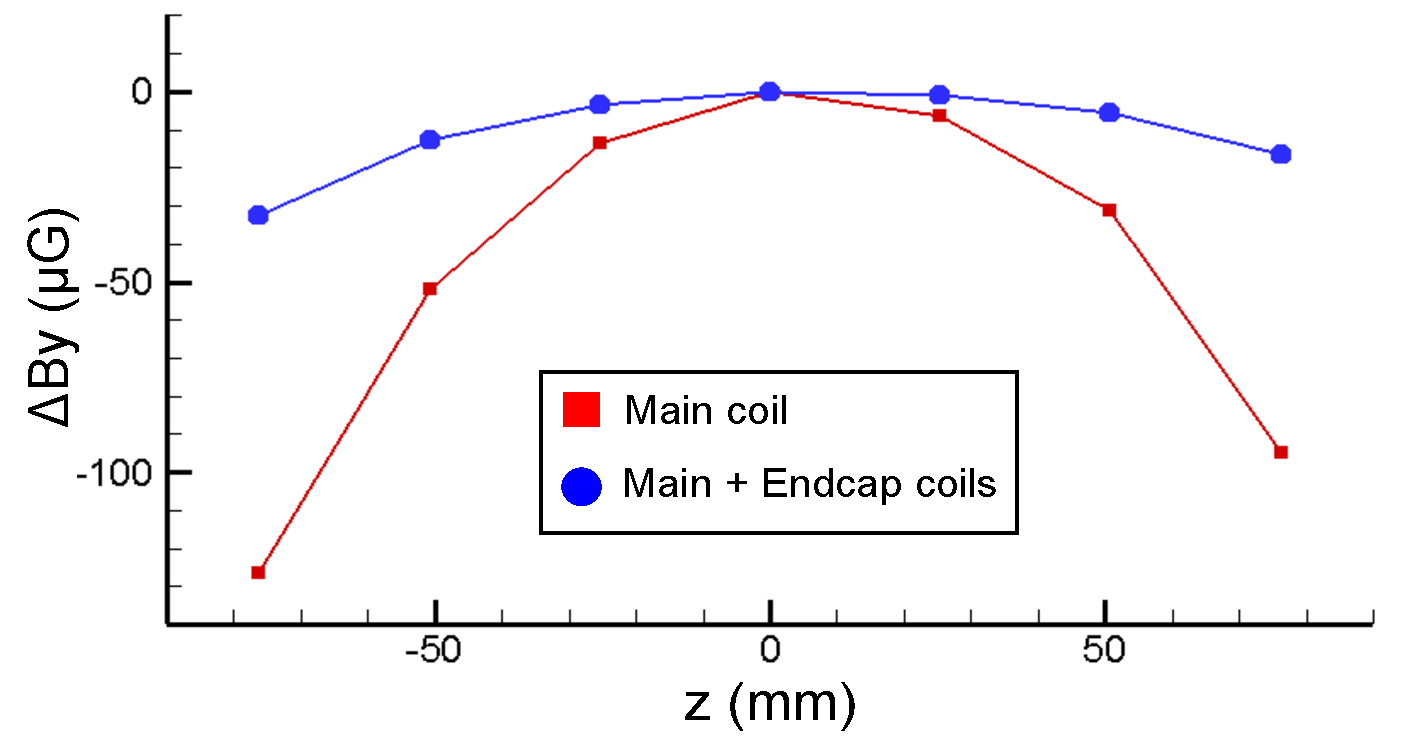
\includegraphics[scale=0.6]{Figures/Fluxgate_By_Measurements.pdf}
\end{center}
\caption[Field map of $\mathbf{B_y}(z)$]%
{\narrower An initial field map of the main magnet coil using a 3-axis fluxgate probe. The map is shown relative to the field in the center of the coil ($z=0$). Without the endcap correction coils, $\mathbf{B_0} = 7.95$ mG (red squares). When the endcap coils were installed in series with the main coil current, $\mathbf{B_0} = 8.29$ mG (blue dots). Linear and quadratic gradients are clearly visible, with the field stronger in the negative z direction (towards the front end of the shields).}
\label{ByMap2010}
\end{figure}

\subsection{Cell motion}
By far the most likely cause for measured HV-correlated frequency differences is cell displacement under the HV within some static gradient field. If the HV exerts some force or mechanical stress on the vessel, the cells may move (individually or as a unit) to some part of the magnet coil with a different average field and different field gradients. If a new sequence began with a resolved HV correlation with $\Delta\omega_{OT-OB}$ and/or $\Delta\omega_{LT}$, the vessel was removed from the apparatus and the nylon bolts which hold the HV feedthroughs in the vessel lids were inspected and adjusted for tightness. The feedthroughs contact the outer cell electrodes, so any expansion, contraction, flexing, tilt, or other motion in the feedthroughs would likely be transmitted to the vapor cells. After a prolonged set of runs during sequence \#7 showed nonzero HV correlation values on the outer cell frequency difference, the top and bottom polyethylene walls of the vessel were removed and replaced with phenolic laminate plates (lined with a thin layer of conducting plastic on the inner surface) to provide extra mechanical rigidity and prevent any HV-generated force from distorting the walls of the vessel. At this point, most of the nylon bolts in the feedthroughs and the vessel walls were replaced with titanium for the same reason.\footnote{Sequence \#7 is also included in the set of auxiliary data to constrain the effect of cell motion on $\Delta\omega_{EDM}.$}

\subsubsection{Wedged cell}
During data gathering, it was discovered that one of the best-performing cells (marked as cell II) has endcaps which are visibly non-parallel. The wedge angle is approximately 0.08$^{\circ}$, which corresponds to a height difference of 0.05mm across the diameter of the endcap ($\approx$ 37mm). While small, this wedge angle may cause cell II to slide or tilt more than other cells under an applied vertical force from the HV electrodes. 
\begin{table}[ht]
\begin{center} 																						
\caption[Middle cell HV frequency shift by sequence] 
{\narrower The HV-correlated frequency shifts observed during each sequence for combinations involving only one cell with non-zero electric field. Each channel MT$\Delta\omega$ and MB$\Delta\omega$ are three-cell combinations which are insensitive to linear magnetic field gradients: MT$\Delta\omega = (2/3)(\omega_{MT}-\omega_{OT}) + (1/3)(\omega_{MT}-\omega_{OB}) $
MB$\Delta\omega = -(1/3)(\omega_{MB}-\omega_{OT}) - (2/3)(\omega_{MB}-\omega_{OB})$
} \label{Single_cell_EDM_sig}	
\begin{tabular}{ccccc}
\hline \hline 
Sequence & MT cell & MT$\Delta\omega (10^{-10}$s$^{-1})$ & MB cell & MB$\Delta\omega(10^{-10}$s$^{-1})$ \\ [0.5ex]	
\hline                   		
1&IV&  $(-6.82 \pm 7.7)$	&II&	$(-7.32 \pm 7.7)$\\
2&II&  $(-31.70\pm 7.5)$	&IV&	$(17.20 \pm 8.3)$\\
4&V&   $(-8.05 \pm 9.0)$	&IV&	$(-5.20 \pm 8.7)$\\
5&IV&  $(-5.17 \pm 8.2)$	&V&		$(1.28  \pm 7.1)$\\
6&II&  $(-7.35 \pm 6.9)$	&V&		$(-2.29 \pm 6.6)$\\
7&II&  $(2.16  \pm 5.8)$	&V&		$(10.00 \pm 5.5)$\\
8&V&   $(2.50  \pm 6.5)$	&II&	$(-2.05 \pm 6.1)$\\
9&II&  $(13.10 \pm 6.8)$	&V&		$(-15.6 \pm 6.6)$\\
10&IV& $(6.28  \pm 7.9)$	&V&		$(-7.33 \pm 7.4)$\\
11&V&  $(7.52  \pm 8.8)$	&IV&	$(-6.49 \pm 8.8)$\\
12&IV& $(-9.45 \pm 9.4)$	&II&	$(-0.98 \pm 9.2)$\\
13&II& $(-4.04 \pm 7.2)$	&IV&	$(-7.48 \pm 7.2)$\\
14&V&  $(-27.30\pm 8.3)$	&II&	$(28.50 \pm 8.3)$\\
Average:&&  $(-4.24\pm 2.1)$&&		$(-0.02 \pm 2.0)$\\
[1ex]	
\hline
\end{tabular}
\end{center} 														
\end{table}

The effect of the cell shape on the dataset can be quantified by breaking out the 4-cell EDM signal $\Delta\omega_{EDM}$ into two signals, each of which incorporates one inner cell as well as both outer cells. The middle top 3-cell signal MT$\Delta\omega = (2/3)(\omega_{MT}-\omega_{OT}) + (1/3)(\omega_{MT}-\omega_{OB})$, while the middle bottom cell signal MB$\Delta\omega = -(1/3)(\omega_{MB}-\omega_{OT}) - (2/3)(\omega_{MB}-\omega_{OB})$. The sum of MT$\Delta\omega$ and MB$\Delta\omega$ is equivalent to the 4-cell EDM signal, and each can be used to examine individual cells for anomalous behavior under voltage. Table \ref{Single_cell_EDM_sig} gives the values of MT$\Delta\omega$ and MB$\Delta\omega$ signals. Table \ref{Single_cell_EDM_AVG} gives the averaged 3-cell signal value for each of the cells used in the center positions; none of the cells has a well-resolved signal, and cell II agrees well with the two cells that have more parallel endcaps, so the wedged endcaps are not likely to be the primary cause of cell motion.

\begin{table}[ht]
\begin{center} 																				
\caption[Average HV frequency shift by cell] 
{\narrower The value of single-cell EDM frequency shifts averaged across all sequences for each cell. The two signals MT$\Delta\omega$ and MB$\Delta\omega$ include a relative sign change so that they can be averaged independently of cell position.} \label{Single_cell_EDM_AVG}	
\begin{tabular}{cc}
\hline \hline 
Cell Number & Average 3-cell $\Delta\omega$ \\ [0.5ex]	
\hline     
II&$(-1.24\pm 2.4)\cdot10^{-10}$\\
IV&$(-2.03\pm 2.9)\cdot10^{-10}$\\
V&$(-2.89\pm 2.4)\cdot10^{-10}$\\          		
[1ex]	
\hline
\end{tabular}
\end{center} 														
\end{table}

While the 4-cell EDM combination removes linear and quadratic field gradients, each 3-cell signal is sensitive to HV-correlated shifts in the second-order magnetic field gradient across the cell stack. Table \ref{Single_cell_EDM_sig} shows that multiple sequences have well-resolved 3-cell EDM-like signals of opposite sign for MT$\Delta\omega$ and MB$\Delta\omega$, which are mostly canceled when the the two signals are summed to the 4-cell EDM value. This behavior is consistent with a quadratic field gradient in the vertical direction $\partial^2 B_y/\partial y^2$ which varies with cell or vessel position. In addition, the 3-cell signals are inconsistent from sequence to sequence, which suggests that the pattern of cell motion is idiosyncratic with each sequence, and is likely to be driven by the different mechanical stresses within the vessel each time the cells are re-arranged, the HV feedthroughs are situated, and the apparatus is put back together. It is also worth noting that during the course of data taking, relatively little attention was paid to the 3-cell signals as indicators of a potential systematic because each incorporates one half of the blind offset used for the 4-cell signal. While experience with the HV-correlated $\Delta\omega_{OT-OB}$ signals during the initial runs of sequence 7 was enough to reject these runs and prompt a re-design of the top and bottom parts of the vessel, sequences with resolved 3-cell signals were tolerated and therefore appear throughout the dataset.

\subsubsection{Dependence on $\mathbf{B_0}$ direction}
Because a real EDM signal changes sign under reversal of both $\mathbf{E}$ and $\mathbf{B_0}$, only a HV-correlated shift in the frequency difference $\Delta\omega_{MT-MB}$ which reverses with the main magnet coil current will systematically alter the measured EDM value.
\begin{figure}
\begin{center}
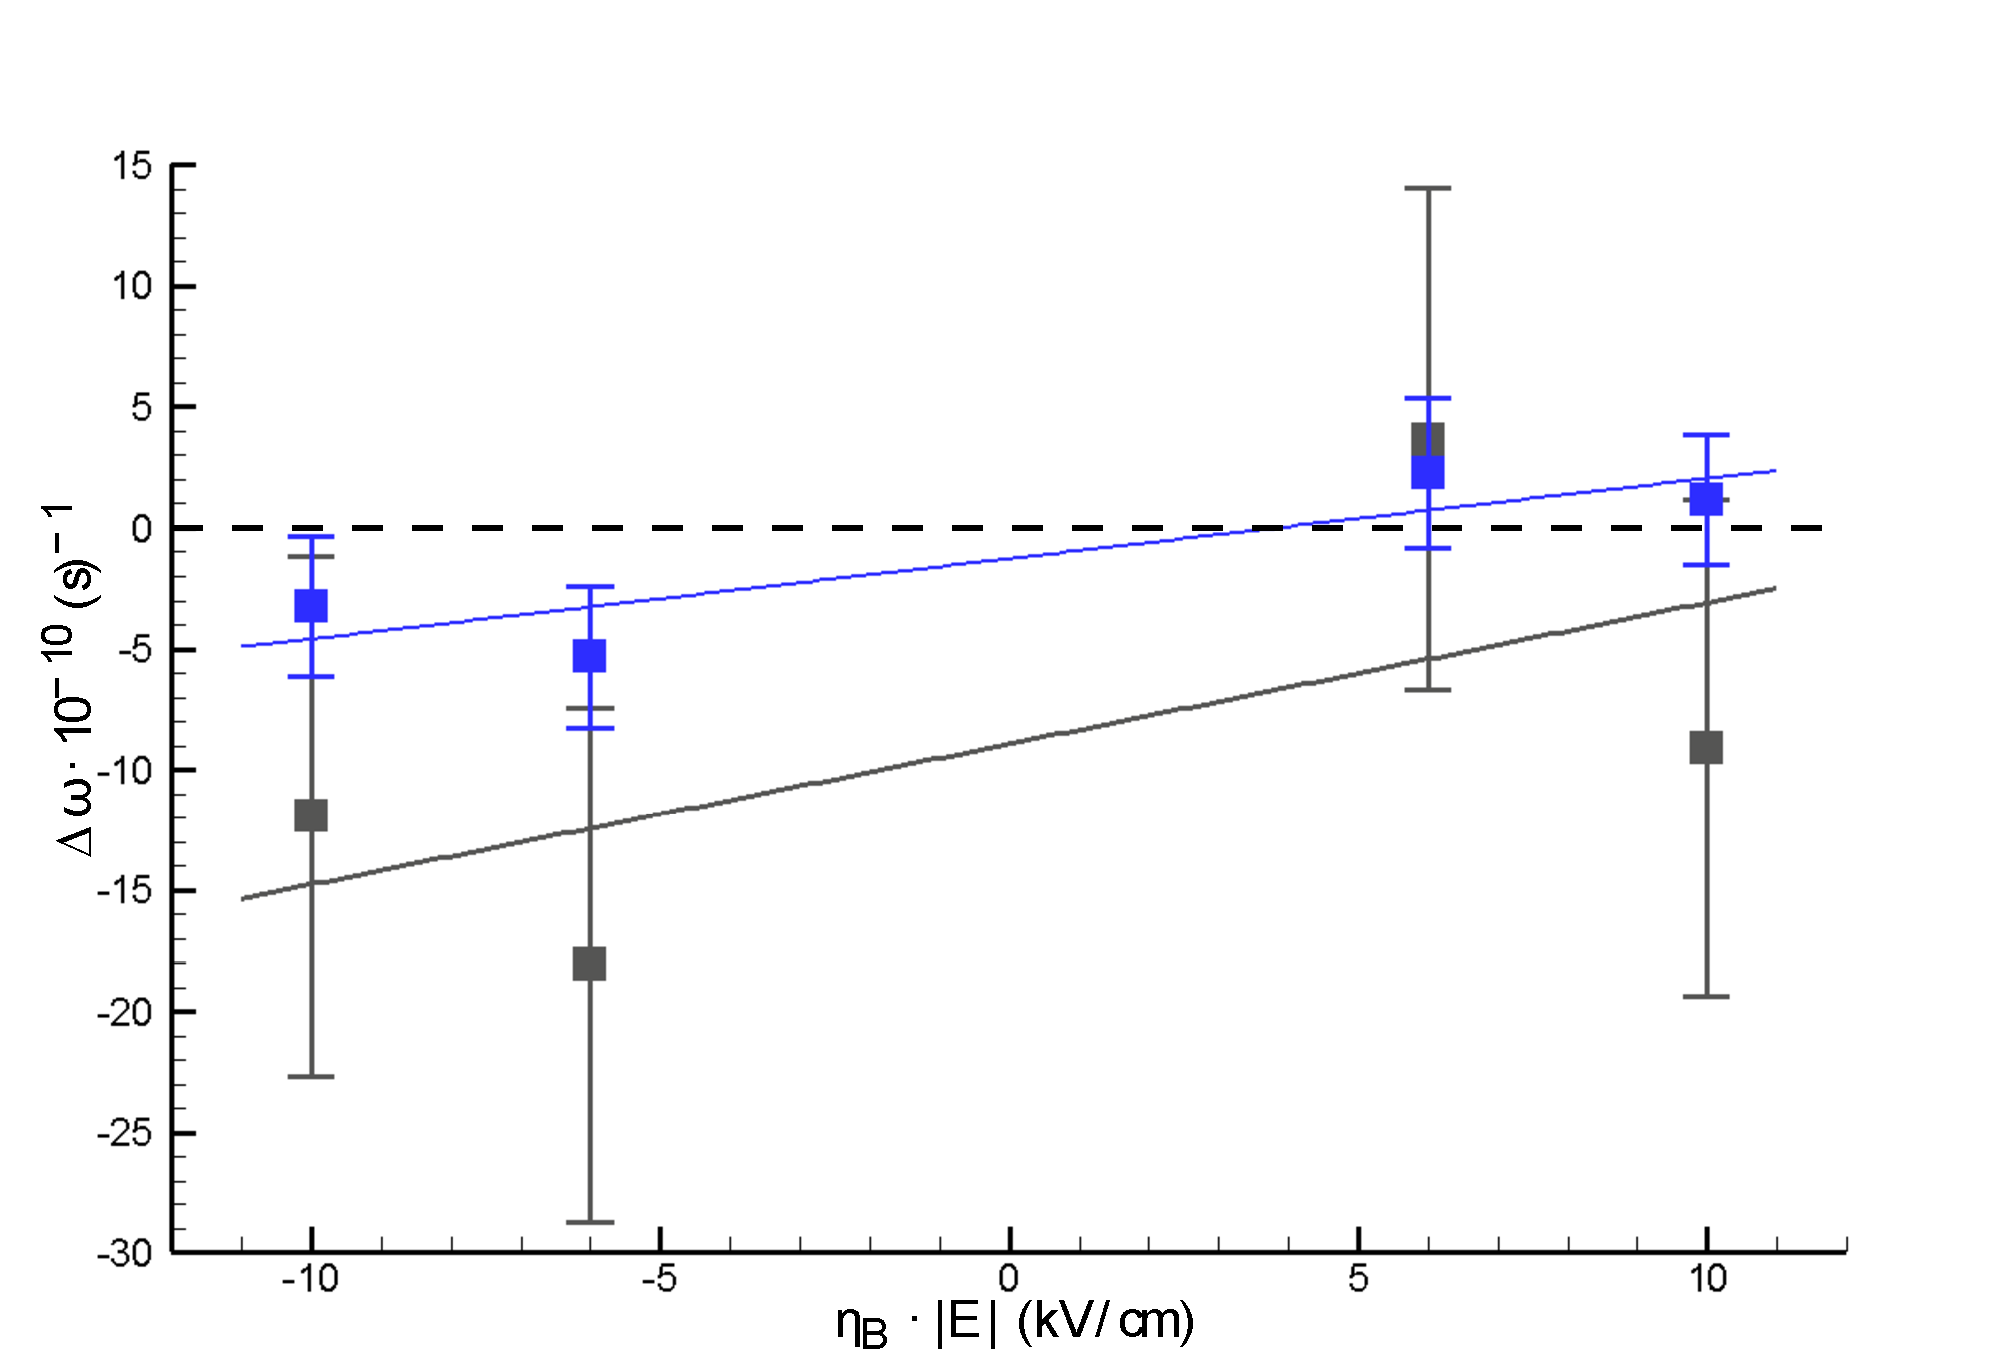
\includegraphics[scale=0.42]{Figures/Unscaled_EDM_OT-OB_Results.pdf}
\end{center}
\caption[$\Delta\omega_{EDM}$ and $\Delta\omega_{OT-OB}$ frequency shifts vs. field configuration]
{\narrower HV-correlated $\Delta\omega_{EDM}$ (in blue) and $\Delta\omega_{OT-OB}$ (in gray) vs. $\eta_{\mathbf{B_0}}\cdot |\mathbf{E}|$, with error-weighted linear fits. The signature of an EDM would be a fit for $\Delta\omega_{EDM}$ with nonzero slope that intersects the origin, along with $\Delta\omega_{OT-OB}$ values consistent with zero. While the values of $\Delta\omega_{EDM}$ ave opposite sign for the two field directions, the best fit line for the outer cell frequency difference is negative across all field configurations. The offset value of $\Delta\omega_{OT-OB}$ is accounted for by HV-induced motion along the magnet coil axis in a linear $\partial B_y/\partial y$ that changes with $z$. The potential bias in the measured EDM value due to the nonzero average $\Delta\omega_{OT-OB}$ is incorporated into the axial cell motion systematic, which is the dominant contribution to the systematic error budget.}
\label{Frequency_Shifts}
\end{figure}
This point may be illustrated by defining the magnetic field direction $\eta_{\mathbf{B}} = \mathbf{B}_0 \cdot \hat{y}/|\mathbf{B}_0| = \pm 1$ and plotting the measured $\Delta \omega_{EDM}$ (defined always as the value of $\Delta\omega_{MT-MB}$ for positive HV minus the same for negative HV) vs. the value of $\eta_{\mathbf{B}}|\mathbf{E_+}-\mathbf{E_-}|$. The relevant data are given in Table \ref{Results}. The signature of a non-zero EDM would be a straight line through the origin, with frequency shifts of equal magnitude with opposite sign for the different magnetic field directions $\eta_{\mathbf{B}}$. However, we find that there is a frequency shift component which appears independent of the magnetic field direction, indicating that at least some of the effect of cell motion does not influence the measured EDM value.

\begin{table}[ht]
\begin{center}													% h = 'here'
\caption[Average HV frequency shift by field configuration] 
{\narrower Measured HV-correlated frequency shifts for various field configurations, normalized by $\mathbf{E}$-field strength. Entries for $\Delta\omega$ are specified in units of $10^{-11}$ (kVs/cm)$^{-1}$.}
\begin{tabular}{cccc}													% centered columns (4 columns) 
\hline \hline	 														% inserts double horizontal lines 
Voltage & $\mathbf{B_0} \cdot \hat{y}$ & $\eta_{\mathbf{B}}\cdot\Delta\omega_{EDM}$ & $\eta_{\mathbf{B}}\cdot\Delta\omega_{OT-OB}$ \\ %header
\hline																	% inserts single line
$\pm$10 kV & +10 mG & $(1.16\pm2.6)$  & $(-8.8\pm9.9)$ \\ 
$\pm$ 6 kV & +10 mG & $(3.69\pm5.0)$  & $(5.9\pm16.7)$ \\  
$\pm$ 6 kV & -10 mG & $(-8.56\pm4.7)$ & $(-29.1\pm17.1)$ \\ 
$\pm$10 kV & -10 mG & $(-3.15\pm2.8)$ & $(-11.5\pm10.4)$ \\ 
\hline
\textbf{Average:} && $(-1.34\pm1.67)$ & $(-10.39\pm6.15)$ \\
\hline
\end{tabular} 
\label{Results} 									
\end{center}
\end{table} 

The impact of cell motion on the EDM dataset is determined by the magnitude of the $\mathbf{B}$-field gradients inside the apparatus and the extent to which these gradients reverse with the direction of coil current. If there is cell motion due to the application of HV, a field gradient that reverses sign with the direction of $\mathbf{B_0}$ will generate a HV-correlated frequency shift $\Delta\omega_{MT-MB}$ that does \textbf{not} change sign with the magnet coil current. This point is illustrated in Figure \ref{Reversible_dBy}: because the precession frequency couples to the magnitude of the total field, and gradients which reverse with $\mathbf{B_0}$ maintain the strength of the field at all points, the change in the frequency difference for any HV-induced displacement is constant. By contrast, gradients which do \textbf{not} change sign with the direction of $\mathbf{B_0}$ will add constructively to $\mathbf{B_0}$ in one direction and destructively in the other. This superposition will change the magnitude of the field at any point based on the direction of $\mathbf{B_0}$, leading to a frequency shift that reverses with magnet coil current. 

\begin{figure}
\begin{center}
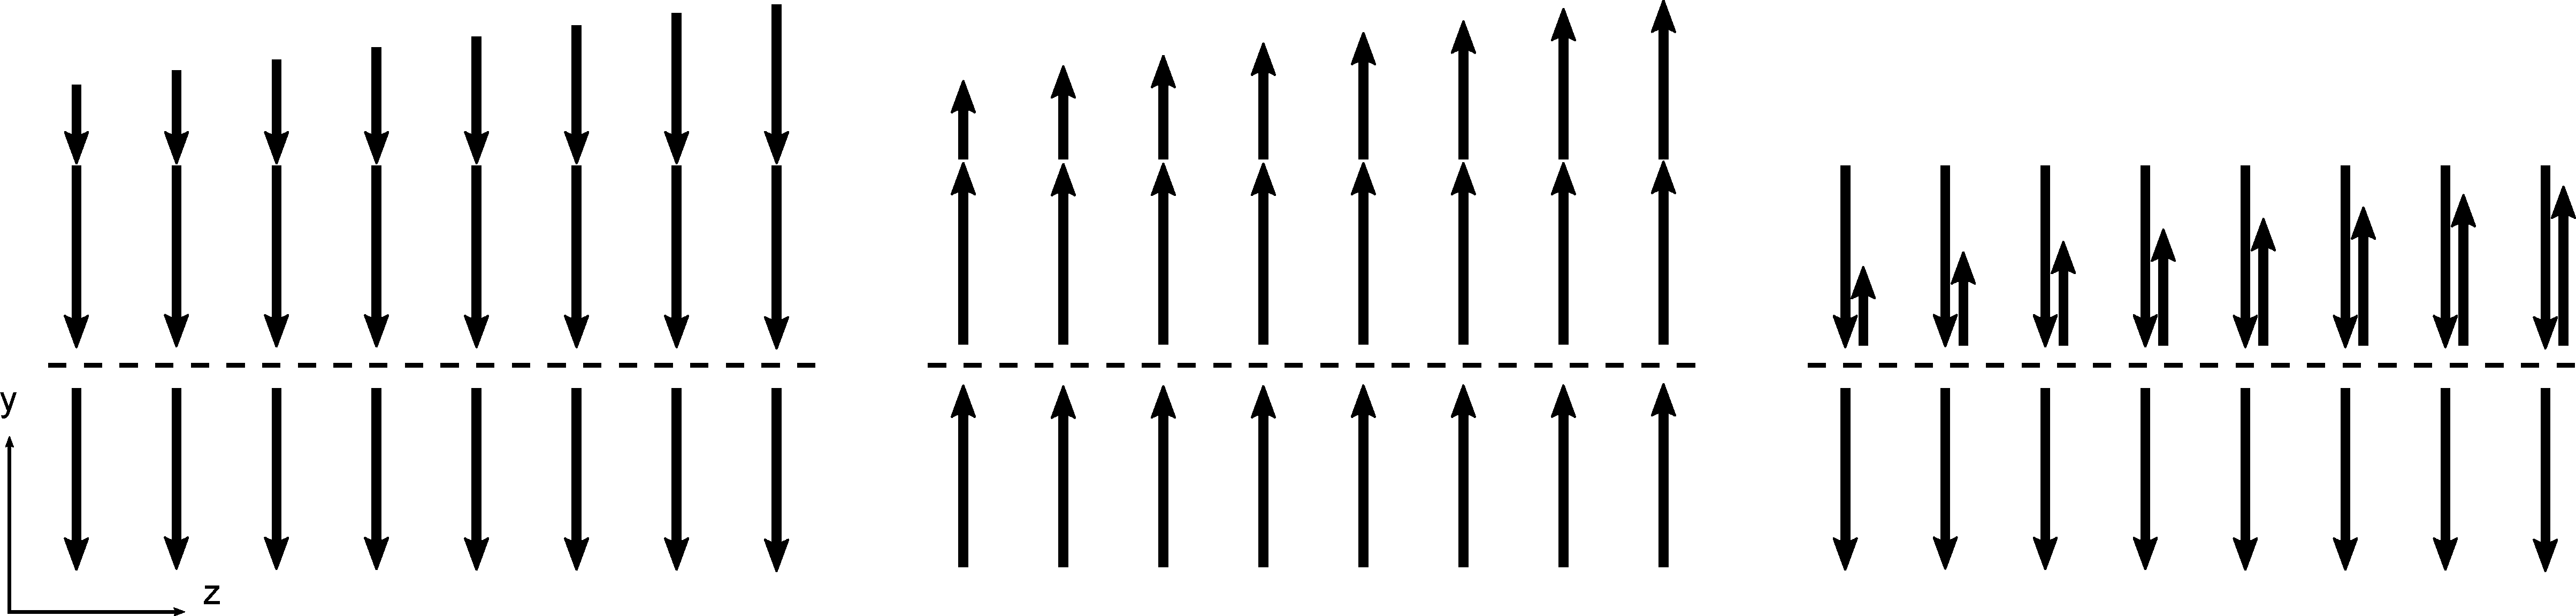
\includegraphics[scale=0.175]{Figures/(Ir)reversible_dBy.pdf}
\end{center}
\caption[Diagram of reversible vs. irreversible vertical field gradients]
{\narrower Simplified representation of reversible vs. irreversible gradients $(\partial/\partial z)(\nabla B_y\cdot\hat{y})$. Center: the vertical gradient $\nabla B_y\cdot\hat{y}$ is positive everywhere and increases with $z$. Left: on reversal of $\mathbf{B_0}$, the gradient also reverses and $\nabla B_y\cdot\hat{y}$ becomes more negative with increasing $z$. The frequency difference between top and bottom cells is thus independent of the direction of $\mathbf{B_0}$ for any given value of $z$, so the periodic $\mathbf{B_0}$ reversals decouple the average change in $\Delta\omega_{MT-MB}$ from any motion induced by the HV. Right: $(\partial/\partial z)(\nabla B_y\cdot\hat{y})$ is independent of $\mathbf{B_0}$; the field magnitude $B_y$ seen by the top cell decreases with $z$. This behavior leads to a frequency difference $\Delta\omega_{MT-MB}$ that changes sign with the direction of $\mathbf{B_0}$, causing HV-correlated cell motion to generate a false EDM signal.}
\label{Reversible_dBy}
\end{figure}

Taking error-weighted average values for each field direction from Table \ref{Results}, the frequency difference signals can be decomposed into $\mathbf{B_0}$-dependent and $\mathbf{B_0}$-independent parts using linear combinations of up and down. The results are given in Table \ref{B_even_odd}. Combined with detailed information on the gradients inside the apparatus, these signals can be used to constrain the effect that cell motion in a given direction may have on the measured EDM value.

\begin{table}													
\begin{center}																					
\caption[Frequency difference channel dependence on $\mathbf{B_0}$ direction] 
{\narrower Averaged values of frequency differences in the EDM dataset for each $\mathbf{B_0}$ direction. $(1/2)(\uparrow + \downarrow)$ isolates the $\mathbf{B_0}$-independent or ``B-even" piece of the signal, while $(1/2)(\uparrow - \downarrow)$ corresponds to the change induced by flipping $\mathbf{B_0}$, or the ``B-odd" piece of the signal.}
\begin{tabular}{cccc}													% centered columns (5 columns) 
\hline \hline	
$\mathbf{B_0}$                 &      OT-OB (kVs/cm)$^{-1}$       &       EDM (kVs/cm)$^{-1}$           \\ \hline
$\uparrow$                     & $(-4.99 \pm 8.44)\cdot10^{-11}$  & $(1.70 \pm 2.31)\cdot10^{-11}$  \\
$\downarrow$                   & $(-16.21 \pm 8.86)\cdot10^{-11}$ & $(-4.57 \pm 2.41)\cdot10^{-11}$ \\
$(1/2)(\uparrow + \downarrow)$ & $(5.61 \pm 6.11)\cdot10^{-11}$   & $(3.13 \pm 1.66)\cdot10^{-11}$  \\
$(1/2)(\uparrow - \downarrow)$ & $(-10.60 \pm 6.11)\cdot10^{-11}$ & $(-1.43 \pm 1.66)\cdot10^{-11}$ \\
\hline
\end{tabular}
\label{B_even_odd} 									
\end{center}
\end{table}


\subsubsection{Field gradient measurements}
After the EDM dataset was complete, a jig was constructed to translate the vessel repeatably in the horizontal and vertical directions, and the vertical gradients were measured across the 4-cell stack in different positions and field directions. Table \ref{Field_gradient_map_x} summarizes the results obtained for changes in vertical gradients as the vessel was moved in the horizontal direction, $(\partial/\partial x)(\nabla B_y\cdot\hat{y})$. The `EDM coupling' results are defined as the ratio of EDM cell frequency difference shifts to outer cell frequency difference shifts. With this ratio, the expected change in $\Delta\omega_{EDM}$ due to to cell motion can be calculated from the measured $\Delta\omega_{OT-OB}$. 

\begin{table} [h]												
\begin{center}											
\caption[Field gradient measurements $(\partial/\partial x)(\nabla B_y\cdot\hat{y})$] 
{\narrower Change in angular frequency differences for vessel displacement of 10mm along $\hat{x}$. For each field configuration, the tabulated values represent the shift in the measured frequency difference when the vessel is translated 5mm in or out of the centered position along the probe beam axis.}
\begin{tabular}{ccccc}													% centered columns (5 columns) 
\hline \hline														
$\mathbf{B_0}$                 & $\Delta\omega_{OT-OB}$ (s$^{-1}$) & $\Delta\omega_{LT}$ (s$^{-1}$)& $\Delta\omega_{EDM}$ (s$^{-1}$) & $\frac{OT-OB}{EDM}$ \\ \hline      
$\uparrow$                     & $-1.40\cdot10^{-3}$ & $-3.57\cdot10^{-4}$ & $6.59\cdot10^{-5}$  & -4.71\%          \\
$\downarrow$                   & $-1.14\cdot10^{-3}$ & $-4.13\cdot10^{-4}$ & $7.02\cdot10^{-5}$  & -6.16\%          \\
$(1/2)(\uparrow + \downarrow)$ & $-1.27\cdot10^{-3}$ & $-3.85\cdot10^{-4}$ & $6.81\cdot10^{-5}$  & \textbf{-5.35\%} \\
$(1/2)(\uparrow - \downarrow)$ & $-1.30\cdot10^{-4}$ & $2.82\cdot10^{-5}$  & $-2.15\cdot10^{-6}$ & \textbf{1.69\%}  \\
\hline
\end{tabular} 
\label{Field_gradient_map_x} 									
\end{center}
\end{table}

Along the $\hat{x}$ direction, the third order gradient is smaller than the linear gradient by a factor of 20. Because the non-reversing part of the linear gradient is dominant, the systematic contribution to the $\Delta\omega^{odd}_{EDM}$ channel can be constrained by the `B-even' part of $\Delta\omega_{OT-OB}$. Denoting the change in the frequency difference between $x$-positions as $\Delta^2\omega$, we have
\begin{equation}
\Delta\omega^{odd}_{EDM} = \Delta\omega^{even}_{OT-OB} \dfrac{\Delta^2\omega^{odd}_{EDM}}{\Delta^2\omega^{even}_{OT-OB}}.
\end{equation}
While the value for $\Delta^2\omega^{odd}_{EDM}$ in Table \ref{Field_gradient_map_x} is on the order of $10^{-6}$, the change in the variable-coefficient EDM signal $\Delta^2\omega_{MT-MB} - k\Delta^2\omega_{OT-OB}$ is $1.09\cdot10^{-5}$(s$^{-1}$). Using this more conservative value for the third-order gradient shift, the expected EDM frequency shift is
\begin{equation}
\Delta\omega^{odd}_{EDM} = (5.60\pm6.11)\cdot10^{-11} \times \dfrac{1.09\cdot10^{-5}}{-1.27\cdot10^{-3}} = (4.80\pm5.23)\cdot10^{-13} \text{(kVs/cm)}^{-1}.
\end{equation}
The systematic contribution is taken to be the 1-$\sigma$ limit of the frequency shift: 
\begin{equation}
\delta d_x = (\hbar/4) \times 1.00 \cdot10^{-12} \text{(kVs/cm)}^{-1} =  1.65\cdot10^{-31} e\cdot \text{cm}.
\end{equation}

\begin{table} [h]													
\begin{center}																					
\caption[Field gradient measurements $(\partial/\partial y)(\nabla B_y\cdot\hat{y})$] 
{\narrower Change in angular frequency differences for vessel displacement of 2mm along $\hat{y}$. The vessel is translated 1mm in or out of the centered position along the vertical axis.}
\begin{tabular}{ccccc}													% centered columns (5 columns) 
\hline \hline									
$\mathbf{B_0}$                 & $\Delta\omega_{OT-OB}$ (s$^{-1}$) & $\Delta\omega_{LT}$ (s$^{-1}$) & $\Delta\omega_{EDM}$ (s$^{-1}$) & $\frac{OT-OB}{EDM}$ \\ \hline      
$\uparrow$                     & $4.88\cdot10^{-4}$  & $-1.50\cdot10^{-6}$ & $-3.35\cdot10^{-4}$ & -68.6\%          \\
$\downarrow$                   & $5.26\cdot10^{-4}$  & $-9.00\cdot10^{-6}$ & $-3.50\cdot10^{-4}$ & -66.6\%          \\
$(1/2)(\uparrow + \downarrow)$ & $5.07\cdot10^{-4}$  & $-5.25\cdot10^{-6}$ & $-3.43\cdot10^{-4}$ & \textbf{-67.6\%} \\
$(1/2)(\uparrow - \downarrow)$ & $-1.90\cdot10^{-5}$ & $3.75\cdot10^{-6}$  & $7.83\cdot10^{-6}$  & \textbf{-0.99\%} \\
\hline
\end{tabular}
\label{Field_gradient_map_y} 									
\end{center}
\end{table}

Unlike the field gradient scans in $x$, the change in the third-order vertical gradients with $y$ is comparable to that of the linear gradient, while the quadratic gradient (proportional to $\Delta\omega_{LT}$) is suppressed relative to either. This behavior is due to the quadratic correction coil $\partial^2B_y/\partial y^2$, shown in Figure \ref{Coil_Currents_On_Axis}. The windings are placed such that the second-order gradient created by the primary coil is locally canceled near the center by the comparatively large fourth-order correction coil gradient in the opposite direction. While signals that incorporate the difference of two or more cells on opposite sides of the groundplane should take out quadratic and quartic gradients by symmetry, motion in this fourth-order gradient couples explicitly to both $\Delta\omega_{OT-OB}$ and $\Delta\omega_{EDM}$. Appendix \ref{nth_gradient} includes a discussion of this behavior, including the cancellation of lower-order gradients by $\Delta\omega_{EDM}$ even if the vessel moves under HV. 

While the impact of cell motion in $y$ cannot be well constrained by comparing the third-order gradients to the linear gradients, both gradients are largely unchanged by the direction of $\mathbf{B_0}$, indicating that they reverse with the sense of the coil current. Measurements of the vertical field gradient dependence on $y$ indicate that the $\Delta\omega{OT-OB}$ signal reverses to within 3.7\% . Similarly, the the $\Delta\omega_{EDM}$ signal reverses to within 2.3\%. We use the larger value as an upper limit on the reversibility of the fields, and derive the feedthrough onto a $\mathbf{B_0}$-sensitive EDM using the `B-even' part of $\Delta\omega_{EDM}^e = (3.1\pm1.7)\cdot10^{-11}$. The estimated EDM frequency shift due to motion in $\hat{y}$ is then $(3.1\pm1.7)\cdot10^{-11} \times 0.037 = (1.15\pm0.63)\cdot10^{-12} \text{(kVs/cm)}^{-1}$. Taking the 1-$\sigma$ value as an upper limit, the systematic contribution for cell motion along $\hat{y}$ is
\begin{equation}
\delta d_y = (\hbar/4) \times 1.78 \cdot10^{-12} \text{(kVs/cm)}^{-1} =  2.93\cdot10^{-31} e\cdot \text{cm}.
\end{equation}
The systematic contributions of motion in the $x$ and $y$ directions are added in quadrature to give the \textit{Radial Cell Motion} systematic:
\begin{equation}
\delta d_{RCM} = 3.36\cdot10^{-31} e\cdot \text{cm}.
\end{equation}
 
\begin{table} [h]													
\begin{center}																					
\caption[Field gradient measurements $(\partial/\partial z)(\nabla B_y\cdot\hat{y})$] 
{\narrower Change in angular frequency differences for vessel displacement of 10mm along $\hat{z}$. For each field configuration, the tabulated values represent the shift in the measured frequency difference when the vessel is translated 5mm in or out of the centered position along the magnet coil axis.}
\begin{tabular}{ccccc}													% centered columns (4 columns) 
\hline \hline									
$\mathbf{B_0}$                 & $\Delta\omega_{OT-OB}$ (s$^{-1}$) & $\Delta\omega_{LT}$ (s$^{-1}$) & $\Delta\omega_{EDM}$ (s$^{-1}$) & $\frac{OT-OB}{EDM}$ \\ \hline      
$\uparrow$                     & $3.22\cdot10^{-4}$  & $-7.16\cdot10^{-5}$ & $-2.79\cdot10^{-5}$ & -8.67\% \\
$\downarrow$                   & $-6.69\cdot10^{-4}$ & $-4.80\cdot10^{-5}$ & $-2.00\cdot10^{-5}$ & 2.99\%  \\
$(1/2)(\uparrow + \downarrow)$ & $-1.74\cdot10^{-4}$ & $-5.98\cdot10^{-5}$ & $-2.40\cdot10^{-5}$ & \textbf{13.8\%}  \\
$(1/2)(\uparrow - \downarrow)$ & $4.96\cdot10^{-4}$  & $-1.18\cdot10^{-5}$ & $-3.97\cdot10^{-6}$ & \textbf{-0.80\%} \\ \hline
\end{tabular} 
\label{Field_gradient_map_z} 									
\end{center}
\end{table}

The vessel was also translated along the shield axis in the $\hat{z}$ direction to measure $(\partial/\partial z)(\nabla B_y\cdot\hat{y})$. The results are summarized in Table \ref{Field_gradient_map_z}. Unlike the changes in $\nabla B_y\cdot\hat{y}$ when the vessel is moved in $\hat{x}$ or $\hat{y}$, the linear vertical field gradients in $\hat{z}$ are substantially different for the two directions of magnet coil current. This behavior implies that motion under the HV along the coil axis can induce a signal on the $\Delta\omega_{OT-OB}$ channel that does not cancel when data from the two $\mathbf{B}$-field directions are compared. Because the outer cell difference is a direct input to $\Delta\omega_{EDM}$, it appears likely that a residual nonzero average $\Delta\omega_{OT-OB}$ would skew the measured EDM value. However, $\Delta\omega_{EDM}$ was found to reverse much better than $\Delta\omega_{OT-OB}$, indicating that the lab-fixed part of the third order gradient is relatively small. Motion in a purely linear gradient would manifest itself as a nonzero value for $\Delta\omega_{OT-OB}$ and $\Delta\omega_{MT-MB}$, which would cancel for $\Delta\omega_{EDM}$. 

\begin{figure} \begin{center}
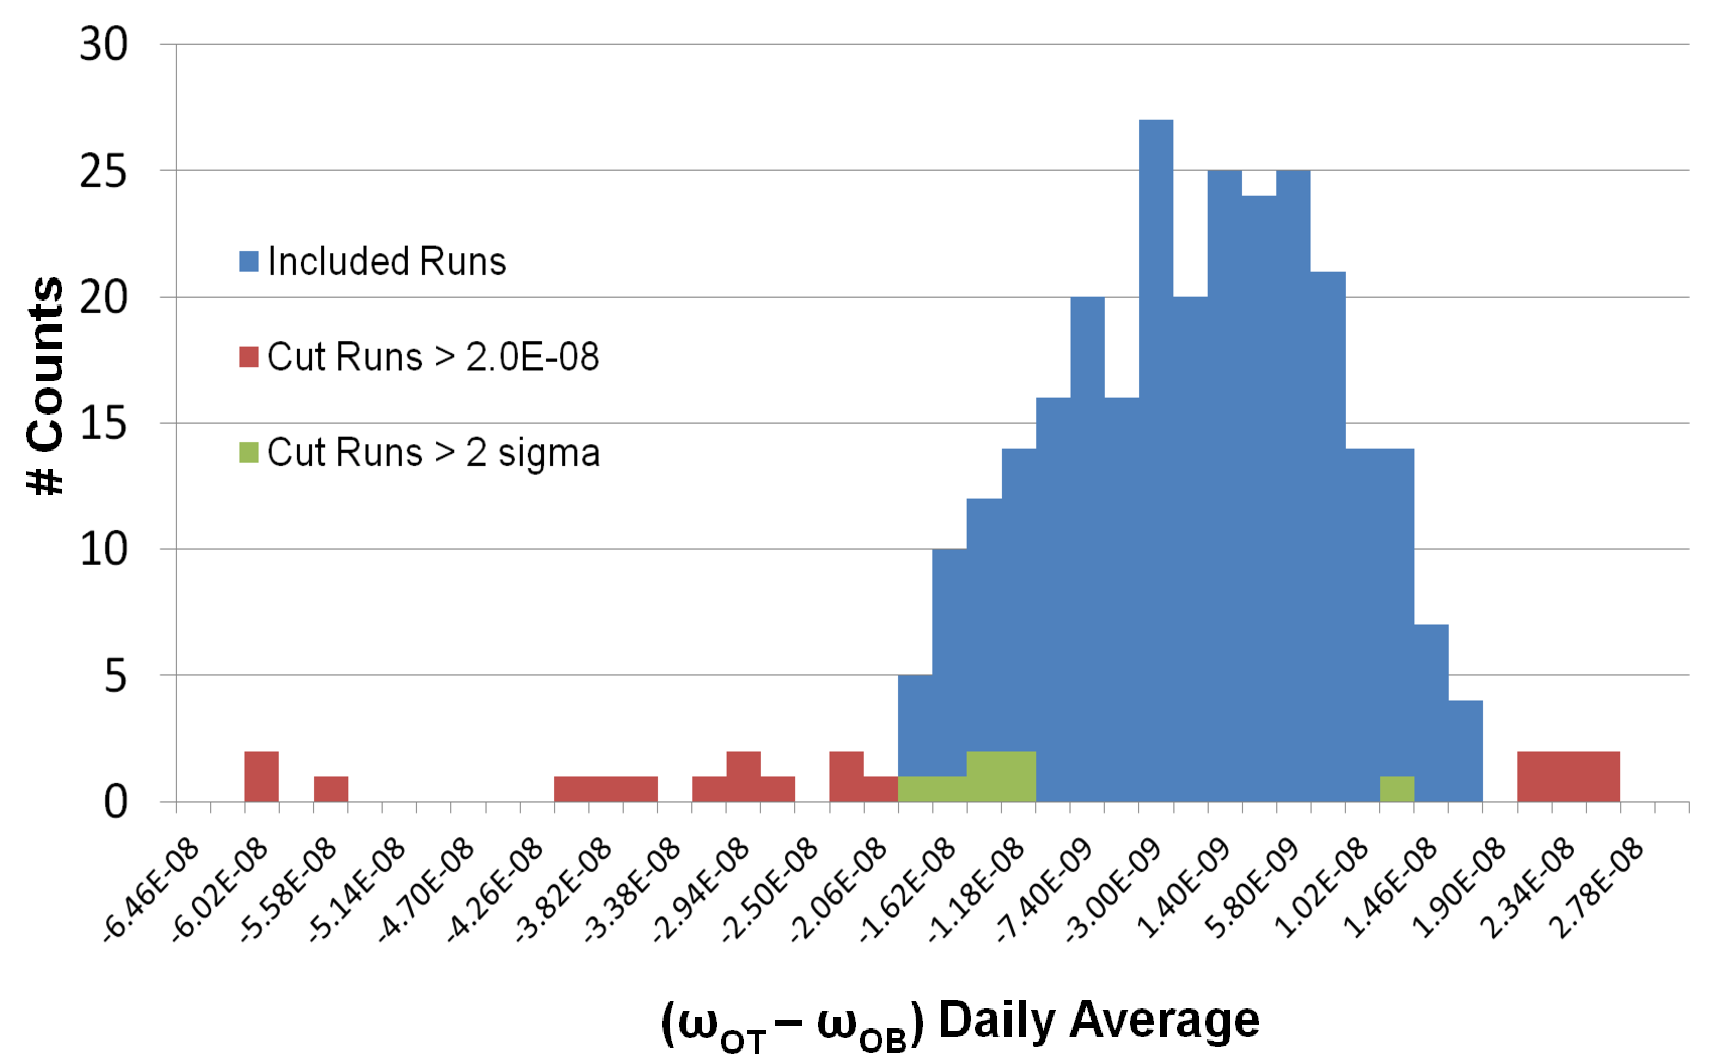
\includegraphics[scale=0.4]{Figures/Outer_Cell_Histogram.pdf}
\end{center}
\caption[Histogram of HV-correlated outer cell frequency difference]%
{\narrower A histogram of the high-voltage-correlated frequency difference $\eta_{\mathbf{B}}\cdot\Delta\omega_{OT-OB}$ for each daily run, accounting for changes in the direction of $\mathbf{B}_0$. Outlying points are clearly skewed towards negative values, which results in a change in the mean value when the data cuts (plotted in red and green) are applied. Several red-plotted runs meet both cut criteria.}
\label{Outer_Cell_Histogram}
\end{figure}
\begin{figure}
\begin{center}
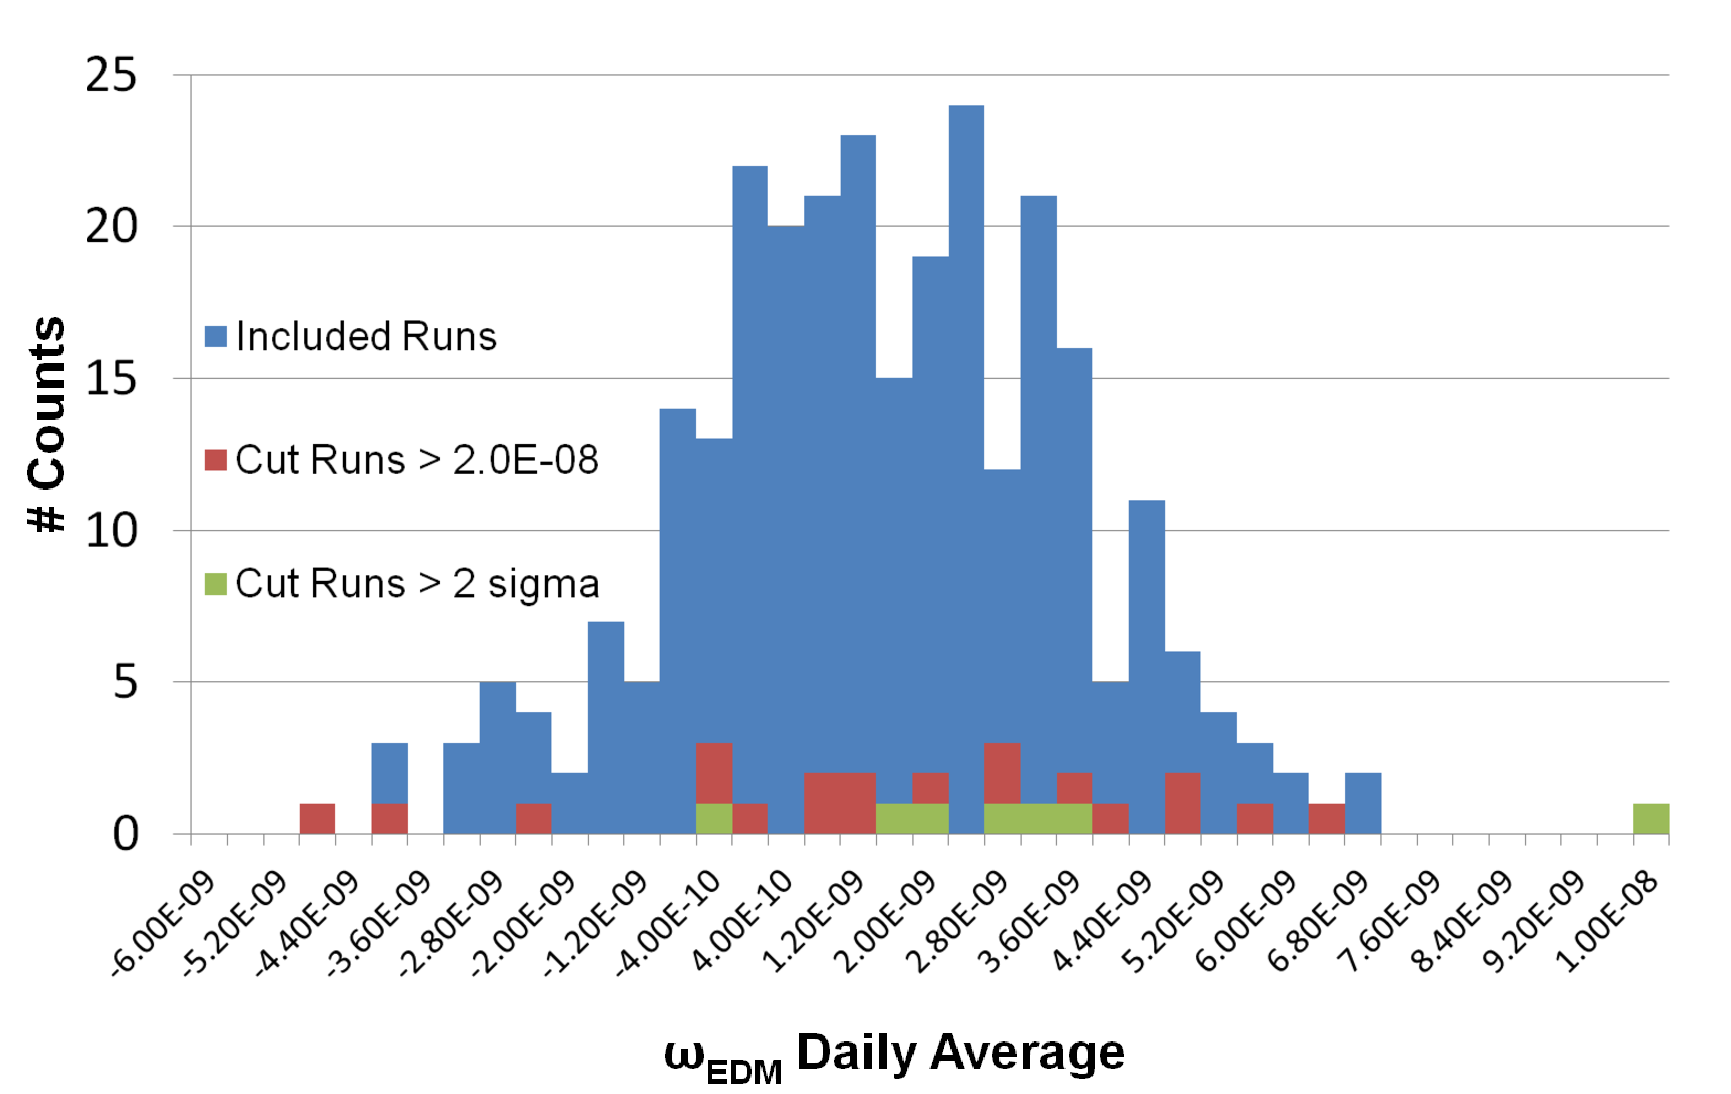
\includegraphics[scale=0.4]{Figures/Combo_Histogram.pdf}
\end{center}
\caption[Histogram of HV-correlated $\Delta\omega_{EDM}$]%
{\narrower A histogram of the high-voltage-correlated EDM frequency difference $\eta_{\mathbf{B}}\cdot\Delta\omega_{EDM}$ for each daily run, accounting for changes in the direction of $\mathbf{B}_0$. The set of cut runs is identical to that of Figure \ref{Outer_Cell_Histogram}, but is distributed across the set of $\Delta\omega_{EDM}$ runs much more uniformly, indicating that the application of data cuts will change the final measured EDM frequency shift much less than the change in $\eta_{\mathbf{B}}\cdot\Delta\omega_{OT-OB}$. This is likely due to cell displacement under HV reversal in a $z$-dependent first-order magnetic field gradient $\partial B_y/\partial y$, which is effectively removed by the 4-cell signal.}
\label{Combo_Histogram}
\end{figure}

Instead of relying on the maps of field gradients in $z$, the systematic contribution of axial cell motion is constrained using the runs that were cut from the final dataset, which are listed in Appendix \ref{Data_Cut_Appendix}. Most of these runs were cut due to unusually large and well resolved daily average values of $\Delta\omega_{OT-OB}$. The set of 95 excluded runs was divided between field directions, and the current-reversing part of $\Delta^{ex}\omega^{odd}_{OT-OB} = (-10.04\pm2.24)\cdot 10^{-9} \text{(s)}^{-1}$. For the included runs, the current-reversing $\Delta^{in}\omega^{odd}_{OT-OB} = (1.18\pm0.63)\cdot 10^{-9} \text{(s)}^{-1}$. The exaggerated change of $\Delta\omega_{OT-OB}$ between field directions for the set of excluded runs presents a natural measurement of the relative impact of non-reversing gradients on $\Delta\omega_{OT-OB}$ and $\Delta\omega_{EDM}$. The feedthrough of a ``$\mathbf{B}$-odd'' change in $\Delta\omega^{odd}_{OT-OB}$ onto $\Delta\omega^{odd}_{EDM}$ is calculated from the difference in average values between included and excluded runs:
\begin{equation}
R =\dfrac{\Delta^{ex}\omega^{odd}_{EDM} - \Delta^{in}\omega^{odd}_{EDM}}{\Delta^{ex}\omega^{odd}_{OT-OB} - \Delta^{in}\omega^{odd}_{OT-OB}}
\end{equation}
\begin{equation}
R =\dfrac{[(1.58\pm0.47) - (1.72\pm0.17)]\cdot 10^{-9} \text{(s)}^{-1}}{[(-10.04\pm2.24) - (1.18\pm0.63)]\cdot 10^{-9} \text{(s)}^{-1}} = (1.6\pm5.7)\text{\%}.
\end{equation}
This systematic constraint is illustrated in Figures \ref{Outer_Cell_Histogram} and \ref{Combo_Histogram}. The outlying daily averages for $\eta_{\mathbf{B}}\cdot\Delta\omega_{OT-OB}$ are obviously skewed towards negative values, and would bias the average of the dataset if they were not removed. By contrast, the same set of cut runs is distributed more symmetrically on either side of the centroid of $\eta_{\mathbf{B}}\cdot\Delta\omega_{EDM}$. Because the outlying runs on the outer cell difference do not correspond to outlying runs on the EDM frequency difference, the coupling between the two must be weaker than would be expected from the definition of $\Delta\omega_{EDM}$. 

The expected value for the reversing part of the EDM frequency shift $\Delta\omega^{odd}_{EDM}$ due to motion along the coil axis can then be determined using the average in $\eta_{\mathbf{B}}\cdot\Delta\omega_{OT-OB}$ from Table \ref{Results}:
\begin{equation}
\Delta\omega^{odd}_{EDM} = (-10.39 \pm 6.15)\cdot 10^{-11}\text{(kVs/cm)}^{-1} \times (0.016 \pm 0.057) = (-1.66 \pm 6.00)\cdot 10^{-12}\text{(kVs/cm)}^{-1}.
\end{equation}
The 1-$\sigma$ limit on $\Delta\omega^{odd}_{EDM}$ is used to determine the \textit{Axial Cell Motion} contribution to the systematic error budget:
\begin{equation}
\delta d_{ACM} = (\hbar/4)\times |(-1.66 - 6.00)\cdot 10^{-12}|\text{(kVs/cm)}^{-1} = 12.64\cdot 10^{-31} e\cdot \text{cm}.
\end{equation} 

It is worth pointing out that $\eta_{\mathbf{B}}\cdot\Delta\omega_{EDM}$ is decoupled from $\eta_{\mathbf{B}}\cdot\Delta\omega_{OT-OB}$ because the EDM frequency difference removes the effect of motion in a linear gradient. Along $z$, the third-order lab-fixed gradients are much smaller than the first-order gradients, but they are measureable. Therefore, it is possible to compute a correction to the average EDM frequency shift based on the ratio of lab-fixed first-order and third-order gradients (approximately 0.8\%). However, Table \ref{Field_gradient_map_z} suggests that any bias on $\Delta\omega^{odd}_{EDM}$ would be approximately 0.8\% of $10.39\cdot 10^{-11}$ (kVs/cm)$^{-1}$, which is one tenth of the axial cell motion systematic.

Finally, the scale of the HV-correlated motion can be estimated by dividing the non-reversing component of $\Delta\omega_{EDM}$ from Table \ref{B_even_odd} by the largest non-reversing gradient: $(\partial/\partial y)(\nabla B_y\cdot\hat{y})$ from Table \ref{Field_gradient_map_y}. This gives a displacement of $3.1\cdot10^{-11} \text{(s)}^{-1} /( 1.7 \cdot 10^{-4} \text{(s)}^{-1}\text{/mm}) \approx 2\cdot10^{-7} \text{mm}$. Thus, HV-correlated cell motion on the order of 2 nanometers could be sufficient to cause the residual signals on $\Delta\omega_{EDM}.$ 

\section{Leakage currents} \label{leakage_systematic}
As mentioned in Chapter \ref{Leakage_methodology}, the measured steady-state currents to the top and bottom groundplanes were each $\le 40$ fA. Using this value for an upper limit on the leakage currents, the impact on $\Delta\omega_{EDM}$ follows from considerations presented in \cite{2009_Hg_EDM}: the average leakage current per cell was 420 fA, and the cell stems are assumed to be stopping points for helical leakage currents, so the ``worst-case current path" consists of $1/2$ turn around each of the middle cells. The current can take a path in either direction around the cell ($\curvearrowleft$ or $\curvearrowright$), so the effect on the EDM frequency difference should add in quadrature. The currents are assumed to be equal on both middle cells, so 420 pA $\cdot \sqrt{2}$ = 590 pA. Each cell is also assumed to have its' own idiosyncratic preferred path for leakage currents. Four cells were the primary contributors to the error-weighted average EDM, so the effect of the currents is divided by 2. This 295 fA effective leakage current yielded a systematic of of $4.53\cdot10^{-30} e\cdot \text{cm}$ as calculated in \cite{2013_Hg_EDM_PRA}. Repeating the above calculation with an average leakage current of 40 fA and three vapor cells in the EDM-sensitive positions gives an effective leakage current of $\sqrt{2/3}\cdot\text{40 fA} = \text{32.6 fA}$. This gives a leakage current systematic of 
\begin{equation}
\delta_{LC} = 5.02 \cdot 10^{-31} e\cdot \text{cm}.
\end{equation}

\section{$|\mathbf{E}|$ effects} \label{|E|_effects}
It is possible that some (heretofore unknown) mechanism exists which couples the frequency of precession to the magnitude of the applied electric field $|\mathbf{E}|$, regardless of direction. If the magnitude $|\mathbf{E}|$ is different for the two polarities of the applied voltage, the combination of these effects would produce a frequency shift which appears to reverse with the direction of $\mathbf{E}$. While any effect of $|\mathbf{E}|$ on the frequency would necessarily be small enough to have gone undiscovered until now, the unparalleled sensitivity of the EDM measurement can be substantially biased by even a fraction of the smallest extraneous effects. 

Our strategy to limit the effect of a frequency shift proportional to $|\mathbf{E}|$ has two steps: After each \textit{dipole} EDM data run (with a $+-+-$ HV sequence), shorter \textit{quadrupole} runs (typically 30 pump-probe cycles) are taken with a $+0-0$ HV sequence. The average value of the frequency difference between the $\pm$ 10 kV runs is compared to the average precession frequency difference with $\mathbf{E}=0$ to measure effects which couple the frequency to $|\mathbf{E}|$. After the end of each sequence, the scalar Stark shift (proportional to $\mathbf{E^2}$) is measured at both HV polarities to obtain a limit on the change in $\mathbf{E}^2$ with field reversal.

\begin{table} 
\footnotesize													
\begin{center}
\caption[Top cell quadratic Stark shift results] 
{\narrower Stark shift results from the middle top cell for positive and negative voltage. The average Stark shift difference between HV polarities is 1.05\% $\pm$ 0.90\%.}   
\label{Stark_MT}
\begin{tabular}{cccc}
\hline \hline									
Seq. & +10 kV Stark shift (V) & -10 kV Stark shift (V) & $\Delta \mathbf{E}^2/\mathbf{E}^2$ \\
\hline        	
1   & $-2.29 \cdot 10^{-4} \pm 4.23 \cdot 10^{-6}$ & $-2.25 \cdot 10^{-4} \pm 3.22 \cdot 10^{-6}$ & 1.76\%  \\
2   & $-1.97 \cdot 10^{-4} \pm 5.30 \cdot 10^{-6}$ & $-1.99 \cdot 10^{-4} \pm 6.24 \cdot 10^{-6}$ & -1.01\% \\
4   & $-2.59 \cdot 10^{-4} \pm 10.8 \cdot 10^{-6}$ & $-2.65 \cdot 10^{-4} \pm 12.3 \cdot 10^{-6}$ & -2.29\% \\
5   & $-1.94 \cdot 10^{-4} \pm 5.36 \cdot 10^{-6}$ & $-1.83 \cdot 10^{-4} \pm 8.17 \cdot 10^{-6}$ & 5.83\%  \\
7'  & $-2.80 \cdot 10^{-4} \pm 4.86 \cdot 10^{-6}$ & $-2.73 \cdot 10^{-4} \pm 4.71 \cdot 10^{-6}$ & 2.53\%  \\
8   & $-2.50 \cdot 10^{-4} \pm 5.40 \cdot 10^{-6}$ & $-2.48 \cdot 10^{-4} \pm 5.38 \cdot 10^{-6}$ & 0.80\%  \\
8*  & $-2.51 \cdot 10^{-4} \pm 2.47 \cdot 10^{-6}$ & $-2.58 \cdot 10^{-4} \pm 2.49 \cdot 10^{-6}$ & -2.75\% \\
9   & $-3.09 \cdot 10^{-4} \pm 2.16 \cdot 10^{-6}$ & $-3.11 \cdot 10^{-4} \pm 2.48 \cdot 10^{-6}$ & -0.64\% \\
10  & $-2.91 \cdot 10^{-4} \pm 2.71 \cdot 10^{-6}$ & $-2.95 \cdot 10^{-4} \pm 3.13 \cdot 10^{-6}$ & -1.36\% \\
11  & $-2.12 \cdot 10^{-4} \pm 6.98 \cdot 10^{-6}$ & $-2.13 \cdot 10^{-4} \pm 6.73 \cdot 10^{-6}$ & -0.47\% \\
12  & $-2.58 \cdot 10^{-4} \pm 9.79 \cdot 10^{-6}$ & $-2.60 \cdot 10^{-4} \pm 9.13 \cdot 10^{-6}$ & -0.77\% \\
13' & $-3.13 \cdot 10^{-4} \pm 7.58 \cdot 10^{-6}$ & $-2.90 \cdot 10^{-4} \pm 6.04 \cdot 10^{-6}$ & 7.63\%  \\
13'*& $-3.22 \cdot 10^{-4} \pm 3.69 \cdot 10^{-6}$ & $-3.04 \cdot 10^{-4} \pm 3.79 \cdot 10^{-6}$ & 5.75\%  \\
14  & $-3.29 \cdot 10^{-4} \pm 3.56 \cdot 10^{-6}$ & $-3.30 \cdot 10^{-4} \pm 2.82 \cdot 10^{-6}$ & -0.30\% \\
\hline
\end{tabular}			
\end{center}										
\end{table}

The Stark shift is measured after each EDM data sequence by locking the laser wavelength to the steepest point on the absorption profile of the EDM cells, then ramping the voltage up and down and observing the change in transmitted light as the excited state energy levels shift with $\mathbf{E}^2$. Each middle cell is measured independently for each voltage polarity. The results of the Stark shift analysis are given in Tables \ref{Stark_MT} and \ref{Stark_MB}. We find that the electric field strength in the middle top cell is the same for both voltage polarities to within 0.52\% $\pm$ 0.45\%, and for the middle bottom cell to within 0.47\% $\pm$ 0.70\%.\footnote{The fractional change in the electric field strength $\Delta|\mathbf{E}|/|\mathbf{E}|$ is approximated as 1/2 the change in the scalar Stark shift because the latter is proportional to $\Delta\mathbf{E}^2/\mathbf{E}^2$. } 

\begin{table} 
\footnotesize													
\begin{center}
\caption[Bottom cell quadratic Stark shift results] 
{\narrower Stark shift results from the middle bottom cell for positive and negative voltage. The average Stark shift difference between HV polarities is 0.94\% $\pm$ 1.40\%.}   
\label{Stark_MB}
\begin{tabular}{ccccc}
\hline \hline									
Seq. & +10 kV Stark shift (V) & -10 kV Stark shift (V) & $\Delta \mathbf{E}^2/\mathbf{E}^2$ \\
\hline        	
1   & $-2.40 \cdot 10^{-4} \pm 5.40 \cdot 10^{-6}$ & $-2.43 \cdot 10^{-4} \pm 5.34 \cdot 10^{-6}$ & -1.24\% \\
2   & $-1.92 \cdot 10^{-4} \pm 3.83 \cdot 10^{-6}$ & $-1.92 \cdot 10^{-4} \pm 4.87 \cdot 10^{-6}$ & 0.00\%  \\
4   & $-2.35 \cdot 10^{-4} \pm 8.02 \cdot 10^{-6}$ & $-2.21 \cdot 10^{-4} \pm 9.31 \cdot 10^{-6}$ & 6.14\%  \\
5   & $-1.81 \cdot 10^{-4} \pm 9.75 \cdot 10^{-6}$ & $-2.04 \cdot 10^{-4} \pm 5.41 \cdot 10^{-6}$ & -11.9\% \\
7'  & $-3.12 \cdot 10^{-4} \pm 8.98 \cdot 10^{-6}$ & $-3.10 \cdot 10^{-4} \pm 8.73 \cdot 10^{-6}$ & 0.64\%  \\
8   & $-3.21 \cdot 10^{-4} \pm 14.0 \cdot 10^{-6}$ & $-2.92 \cdot 10^{-4} \pm 13.4 \cdot 10^{-6}$ & 9.46\%  \\
8*  & $ 2.77 \cdot 10^{-4} \pm 2.67 \cdot 10^{-6}$ & $ 2.73 \cdot 10^{-4} \pm 2.56 \cdot 10^{-6}$ & 1.45\%  \\
9   & $ 2.51 \cdot 10^{-4} \pm 2.76 \cdot 10^{-6}$ & $ 2.41 \cdot 10^{-4} \pm 2.53 \cdot 10^{-6}$ & 4.06\%  \\
10  & $-2.28 \cdot 10^{-4} \pm 5.44 \cdot 10^{-6}$ & $-2.28 \cdot 10^{-4} \pm 5.89 \cdot 10^{-6}$ & 0.00\%  \\
11  & $-2.65 \cdot 10^{-4} \pm 6.00 \cdot 10^{-6}$ & $-2.47 \cdot 10^{-4} \pm 6.77 \cdot 10^{-6}$ & 7.03\%  \\
12  & $-3.37 \cdot 10^{-4} \pm 3.31 \cdot 10^{-6}$ & $-3.40 \cdot 10^{-4} \pm 2.73 \cdot 10^{-6}$ & -0.88\% \\
13' & $-2.73 \cdot 10^{-4} \pm 5.02 \cdot 10^{-6}$ & $-2.73 \cdot 10^{-4} \pm 3.14 \cdot 10^{-6}$ & 0.00\%  \\
13'*& $-2.78 \cdot 10^{-4} \pm 3.18 \cdot 10^{-6}$ & $-2.80 \cdot 10^{-4} \pm 3.30 \cdot 10^{-6}$ & -0.71\% \\
14  & $-3.37 \cdot 10^{-4} \pm 3.31 \cdot 10^{-6}$ & $-3.40 \cdot 10^{-4} \pm 2.73 \cdot 10^{-6}$ & -0.88\% \\
\hline
\end{tabular}			
\end{center}										
\end{table}

Results for the quadrupole HV correlation and the electric field reversibility are combined for each cell with nonzero field to produce an estimate of the systematic effect. The frequency combinations used to measure the quadrupole HV correlation isolate one inner cell and a combination of the two outer cells which remove the sensitivity to a linear magnetic field gradient: $\Delta\omega_{MT} = \omega_{MT} - \frac{2}{3}\omega_{OT} - \frac{1}{3}\omega_{OB}$, $\Delta\omega_{MB} = \omega_{MB} - \frac{2}{3}\omega_{OB} - \frac{1}{3}\omega_{OT}$. Finally, the difference in the systematic shifts for the two inner cell frequency combinations is taken as the limit on the HV correlation of the EDM signal $\Delta\omega_{EDM}$ due to changes in the magnitude of $\mathbf{E}$. Averaged over all sequences, the measured effect is $(0.80 \pm 2.24) \cdot 10^{-31}$ $e \cdot \text{cm}$. We use a 1-$\sigma$ limit for the contribution to the EDM systematic error budget: 
\begin{equation}
\delta d_{|\mathbf{E}|} = 3.04 \cdot 10^{-31} e \cdot \text{cm}.  
\end{equation}

\begin{table}[t] 
\footnotesize													
\begin{center}
\caption[$\Delta|\mathbf{E}|$ frequency shift limits] 
{\narrower Results for the systematic frequency shift due to $\Delta|\mathbf{E}|$. Correlation values and systematic values are given in units of angular frequency (s$^{-1}$). The difference between the middle top cell and middle bottom cell systematics are used to determine the correlation between the HV polarity, the electric field strength $|\mathbf{E}|$, and the EDM-sensitive frequency difference $\Delta\omega_{MT-MB}$. Averaged over all sequences, the systematic is $(5.00 \pm 14.0) \cdot 10^{-12}$ s$^{-1}$.}   
\begin{tabular}{c|ccc|ccc|c}
\hline \hline									
Seq. & $\Delta\omega_{MT}$ ($\cdot 10^{-9}$)&$\Delta|\mathbf{E}|/|\mathbf{E}|$ & Systematic & $\Delta\omega_{MB}$ ($\cdot 10^{-9}$)&$\Delta|\mathbf{E}|/|\mathbf{E}|$ & Systematic & Difference \\
\hline 
1    & $-0.67 \pm 2.23 $ &  0.88\% & $-5.88 \cdot 10^{-12}$ & $ 2.59 \pm 2.56$  & -0.62\% & $-1.06 \cdot 10^{-11}$ & $  1.02 \cdot 10^{-11}$\\
2    & $-0.82 \pm 1.61 $ & -0.50\% & $ 4.13 \cdot 10^{-12}$ & $ 3.21 \pm 1.85$  &  0.00\% & $ 0.00 \cdot 10^{-12}$ & $  4.13 \cdot 10^{-12}$\\
4    & $-0.63 \pm 2.73 $ & -1.14\% & $ 7.21 \cdot 10^{-12}$ & $ 3.29 \pm 2.98$  &  3.07\% & $ 1.01 \cdot 10^{-10}$ & $ -9.38 \cdot 10^{-11}$\\
5    & $ 1.46 \pm 2.38 $ &  2.91\% & $ 4.26 \cdot 10^{-11}$ & $ 0.93 \pm 2.34$  & -5.97\% & $-5.53 \cdot 10^{-11}$ & $  9.79 \cdot 10^{-11}$\\
7'   & $-0.79 \pm 1.89 $ &  1.26\% & $-1.00 \cdot 10^{-11}$ & $ 2.63 \pm 1.72$  &  0.32\% & $ 8.46 \cdot 10^{-12}$ & $ -1.84 \cdot 10^{-11}$\\
8    & $-2.65 \pm 2.40 $ &  0.80\% & $-1.06 \cdot 10^{-11}$ & $-1.14 \pm 2.18$  &  4.73\% & $-5.39 \cdot 10^{-11}$ & $  4.33 \cdot 10^{-11}$\\
8*   & $-2.65 \pm 2.40 $ & -1.37\% & $ 3.64 \cdot 10^{-11}$ & $-1.14 \pm 2.18$  &  0.73\% & $-8.29 \cdot 10^{-12}$ & $  4.47 \cdot 10^{-11}$\\
9    & $ 3.34 \pm 2.10 $ & -0.32\% & $-1.08 \cdot 10^{-11}$ & $-4.30 \pm 2.01$  &  2.03\% & $-8.74 \cdot 10^{-11}$ & $  7.66 \cdot 10^{-11}$\\
10   & $-2.07 \pm 2.36 $ & -0.68\% & $ 1.41 \cdot 10^{-11}$ & $-0.06 \pm 2.46$  &  0.00\% & $ 0.00 \cdot 10^{-12}$ & $  1.41 \cdot 10^{-11}$\\
11   & $-2.45 \pm 3.29 $ & -0.24\% & $ 5.76 \cdot 10^{-12}$ & $ 1.85 \pm 3.23$  &  3.52\% & $ 6.50 \cdot 10^{-11}$ & $ -5.93 \cdot 10^{-11}$\\
12   & $ 3.09 \pm 2.95 $ & -0.39\% & $-1.19 \cdot 10^{-11}$ & $-4.14 \pm 3.14$  & -0.44\% & $ 1.83 \cdot 10^{-11}$ & $ -3.03 \cdot 10^{-11}$\\
13'  & $-0.34 \pm 2.46 $ &  3.81\% & $-1.31 \cdot 10^{-11}$ & $-0.46 \pm 2.42$  &  0.00\% & $ 0.00 \cdot 10^{-12}$ & $ -1.31 \cdot 10^{-11}$\\
13'* & $-0.34 \pm 2.46 $ &  2.88\% & $-9.89 \cdot 10^{-12}$ & $-0.46 \pm 2.42$  & -0.36\% & $ 1.64 \cdot 10^{-12}$ & $ -1.15 \cdot 10^{-11}$\\
14   & $ 0.30 \pm 1.88 $ & -0.15\% & $-4.48 \cdot 10^{-13}$ & $ 1.31 \pm 1.83$  & -0.44\% & $-5.80 \cdot 10^{-12}$ & $  5.36 \cdot 10^{-12}$\\
\hline
\end{tabular}			
\end{center}										
\label{|E|_systematic}
\end{table}

\section{Parameter correlations} \label{ParameterCorr}
It is not possible guarantee that all relevant systematic sources of error have been properly accounted for. New and subtle systematic effects relevant to EDM experiments have been discovered in the recent past, including the possibility of errors induced by geometric phase \cite{2004_Geometric_Phase_ILL_nEDM} and gravitational UCN depolarization effects \cite{2015_ILL_nEDM_gravity_correction}. In order to account for the contribution of some unknown mechanism to a field-correlated frequency shift, approximately 30 different parameters were monitored in conjunction with the frequency differences and analyzed for a correlation with $\mathbf{E}\cdot\mathbf{B}$. These parameters were also analyzed for a correlation with the EDM frequency difference signal. The correlation of each parameter with the EDM signal is multiplied by the correlation between the same parameter and $\mathbf{E}\cdot\mathbf{B}$, and the product is used as an estimate of the dependence of the EDM signal on the fields $\mathbf{E}\cdot\mathbf{B}$ mediated by some unknown mechanism associated with the measured parameter. The systematic contributions are added in quadrature because they are assumed to be independent. The final systematic contribution is 
\begin{equation}
\delta d_{PC} = 2.33 \cdot 10^{-31} e\cdot \text{cm}.
\end{equation}

\begin{table}[p] 
\footnotesize													
\begin{center}
\caption[Parameter correlation systematic error estimates] 
{\narrower Correlation values for various parameters of interest with the EDM signal $\Delta\omega_{EDM}$ and the field configuration $\mathbf{E}\cdot\mathbf{B}$. Values in the first column are recorded in units such that they yield a frequency shift when multiplied by the units of the second column. For example, the laser intensity vs. $\mathbf{E}\cdot\mathbf{B}$ is measured in volts on a photodetector, and the second column has units of s$^{-1}$/V, so the product of the correlations is a frequency shift. Limits are taken by adding 1-$\sigma$ to the absolute value of the product.}   
\begin{tabular}{cccccc}
\hline \hline									
Parameter&$\mathbf{E}\cdot\mathbf{B}$ Correlation&$\Delta\omega_{EDM}$ Correlation&Product&Error&1-$\sigma$ limit\\
\hline        	
MT Dark Lifetime	& $ (-2.03 \pm 0.72) \cdot10^{-3} $ & $  (-9.89 \pm 5.37) \cdot10^{-10} $ & $  2.01\cdot10^{-12} $ & $ 1.31\cdot10^{-12} $ & $  3.32\cdot10^{-12} $ \\
MB Dark Lifetime	& $  (2.18 \pm 0.98) \cdot10^{-3} $ & $  (-10.9 \pm 6.36) \cdot10^{-10} $ & $ -2.37\cdot10^{-12} $ & $ 1.75\cdot10^{-12} $ & $  4.12\cdot10^{-12} $ \\
OT Dark Lifetime	& $  (4.28 \pm 3.12) \cdot10^{-4} $ & $  (-2.29 \pm 1.43) \cdot10^{-9}  $ & $ -9.81\cdot10^{-13} $ & $ 9.41\cdot10^{-13} $ & $  1.92\cdot10^{-12} $ \\
OB Dark Lifetime	& $ (-6.81 \pm 2.15) \cdot10^{-4} $ & $  (-16.3 \pm 5.84) \cdot10^{-10} $ & $  1.11\cdot10^{-12} $ & $ 5.30\cdot10^{-13} $ & $  1.64\cdot10^{-12} $ \\
MT Amplitude 		& $  (2.01 \pm 1.51) \cdot10^{-6} $ & $  (-8.54 \pm 7.62) \cdot10^{-7}  $ & $ -1.72\cdot10^{-12} $ & $ 2.00\cdot10^{-12} $ & $  3.72\cdot10^{-12} $ \\
MB Amplitude 		& $  (2.06 \pm 1.27) \cdot10^{-6} $ & $  (-5.11 \pm 6.26) \cdot10^{-7}  $ & $ -1.05\cdot10^{-12} $ & $ 1.44\cdot10^{-12} $ & $  2.50\cdot10^{-12} $ \\
OT Amplitude 		& $  (2.74 \pm 1.75) \cdot10^{-6} $ & $  (-3.99 \pm 5.26) \cdot10^{-7}  $ & $ -1.09\cdot10^{-12} $ & $ 1.60\cdot10^{-12} $ & $  2.70\cdot10^{-12} $ \\
OB Amplitude 		& $  (2.98 \pm 1.46) \cdot10^{-6} $ & $  (-8.39 \pm 4.95) \cdot10^{-7}  $ & $ -2.50\cdot10^{-12} $ & $ 1.92\cdot10^{-12} $ & $  4.42\cdot10^{-12} $ \\
MT Transmission		& $ (-6.40 \pm 6.97) \cdot10^{-6} $ & $   (2.67 \pm 2.50) \cdot10^{-8}  $ & $ -1.71\cdot10^{-13} $ & $ 2.46\cdot10^{-13} $ & $  4.17\cdot10^{-13} $ \\
MB Transmission		& $ (-1.65 \pm 6.12) \cdot10^{-6} $ & $   (3.43 \pm 2.99) \cdot10^{-8}  $ & $ -5.66\cdot10^{-14} $ & $ 2.16\cdot10^{-13} $ & $  2.72\cdot10^{-13} $ \\
OT Transmission		& $ (-4.32 \pm 5.88) \cdot10^{-6} $ & $   (3.04 \pm 2.50) \cdot10^{-8}  $ & $ -1.31\cdot10^{-13} $ & $ 2.09\cdot10^{-13} $ & $  3.40\cdot10^{-13} $ \\
OB Transmission		& $ (-1.24 \pm 5.58) \cdot10^{-6} $ & $   (2.18 \pm 3.14) \cdot10^{-8}  $ & $ -2.70\cdot10^{-14} $ & $ 1.28\cdot10^{-13} $ & $  1.55\cdot10^{-13} $ \\
Laser Int.		& $ (-3.06 \pm 7.91) \cdot10^{-7} $ & $   (9.54 \pm 9.93) \cdot10^{-8}  $ & $ -2.92\cdot10^{-14} $ & $ 8.14\cdot10^{-14} $ & $  1.11\cdot10^{-13} $ \\
Diode Current		& $  (0.67 \pm 4.62) \cdot10^{-8} $ & $   (8.82 \pm 7.42) \cdot10^{-6}  $ & $  5.92\cdot10^{-14} $ & $ 4.10\cdot10^{-13} $ & $  4.70\cdot10^{-13} $ \\
Green Piezo		& $  (0.05 \pm 3.55) \cdot10^{-6} $ & $   (0.64 \pm 3.93) \cdot10^{-9}  $ & $  3.30\cdot10^{-17} $ & $ 2.26\cdot10^{-15} $ & $  2.30\cdot10^{-15} $ \\
UV Piezo		& $  (2.29 \pm 3.12) \cdot10^{-7} $ & $  (-0.54 \pm 2.62) \cdot10^{-9}  $ & $ -1.23\cdot10^{-16} $ & $ 6.22\cdot10^{-16} $ & $  7.45\cdot10^{-16} $ \\
dBy/dy Coil 1		& $  (0.21 \pm 1.64) \cdot10^{-9} $ & $  (-0.57 \pm 3.34) \cdot10^{-4}  $ & $ -1.21\cdot10^{-14} $ & $ 1.18\cdot10^{-13} $ & $  1.30\cdot10^{-13} $ \\
dBy/dy Coil 2		& $  (0.09 \pm 1.37) \cdot10^{-9} $ & $   (1.04 \pm 2.65) \cdot10^{-4}  $ & $  8.94\cdot10^{-15} $ & $ 1.44\cdot10^{-13} $ & $  1.53\cdot10^{-13} $ \\
dBy/dx Coil		& $  (0.11 \pm 2.85) \cdot10^{-9} $ & $   (3.53 \pm 2.69) \cdot10^{-5}  $ & $  3.85\cdot10^{-15} $ & $ 1.01\cdot10^{-13} $ & $  1.04\cdot10^{-13} $ \\
Endcap Coil		& $  (1.71 \pm 2.81) \cdot10^{-9} $ & $  (-0.39 \pm 1.12) \cdot10^{-4}  $ & $ -6.65\cdot10^{-14} $ & $ 2.21\cdot10^{-13} $ & $  2.87\cdot10^{-13} $ \\
Main Coil		& $ (-1.30 \pm 3.40) \cdot10^{-9} $ & $   (0.19 \pm 1.37) \cdot10^{-4}  $ & $ -2.46\cdot10^{-14} $ & $ 1.89\cdot10^{-13} $ & $  2.14\cdot10^{-13} $ \\
External Bx		& $ (-2.41 \pm 2.46) \cdot10^{-5} $ & $  (-13.6 \pm 1.83) \cdot10^{-8}  $ & $  3.28\cdot10^{-12} $ & $ 3.37\cdot10^{-12} $ & $  6.66\cdot10^{-12} $ \\
External By		& $  (0.51 \pm 1.60) \cdot10^{-7} $ & $  (-23.7 \pm 6.62) \cdot10^{-9}  $ & $ -1.20\cdot10^{-15} $ & $ 3.82\cdot10^{-15} $ & $  5.01\cdot10^{-15} $ \\
External Bz		& $ (-13.5 \pm 5.96) \cdot10^{-6} $ & $  (-41.0 \pm 4.49) \cdot10^{-8}  $ & $  5.53\cdot10^{-12} $ & $ 2.52\cdot10^{-12} $ & $  8.05\cdot10^{-12} $ \\
External By (2)*	& $  (0.27 \pm 2.36) \cdot10^{-8} $ & $   (6.47 \pm 4.69) \cdot10^{-7}  $ & $  1.74\cdot10^{-15} $ & $ 1.53\cdot10^{-14} $ & $  1.71\cdot10^{-14} $ \\
Vert. beam disp.	& $  (11.7 \pm 9.62) \cdot10^{-8} $ & $  (-0.69 \pm 1.27) \cdot10^{-6}  $ & $ -8.03\cdot10^{-14} $ & $ 1.62\cdot10^{-13} $ & $  2.43\cdot10^{-13} $ \\
Horiz. beam disp.	& $  (6.70 \pm 9.78) \cdot10^{-8} $ & $  (-0.69 \pm 1.27) \cdot10^{-6}  $ & $ -4.61\cdot10^{-14} $ & $ 1.08\cdot10^{-13} $ & $  1.55\cdot10^{-13} $ \\
Chopper Freq.		& $  (2.21 \pm 4.19) \cdot10^{-6} $ & $   (6.19 \pm 3.56) \cdot10^{-7}  $ & $  1.37\cdot10^{-12} $ & $ 2.71\cdot10^{-12} $ & $  4.08\cdot10^{-12} $ \\
Table Temp.		& $ (-0.48 \pm 1.41) \cdot10^{-6} $ & $  (-13.8 \pm 8.59) \cdot10^{-7}  $ & $  6.58\cdot10^{-13} $ & $ 1.99\cdot10^{-12} $ & $  2.65\cdot10^{-12} $ \\
Laser Temp.		& $ (-0.66 \pm 1.46) \cdot10^{-6} $ & $  (-2.83 \pm 5.52) \cdot10^{-7}  $ & $  1.88\cdot10^{-13} $ & $ 5.53\cdot10^{-13} $ & $  7.40\cdot10^{-13} $ \\
Air Temp.		& $ (-1.34 \pm 1.92) \cdot10^{-5} $ & $  (-4.72 \pm 4.20) \cdot10^{-8}  $ & $  6.31\cdot10^{-13} $ & $ 1.07\cdot10^{-12} $ & $  1.70\cdot10^{-12} $ \\
\hline
\textbf{Quadrature Sum:}		&&&&&	    $\mathbf{1.46\cdot10^{-11} \text{s}^{-1}}$ \\	 
\hline					
\end{tabular}			
\end{center}										
\label{ParameterCorrelations}
\end{table}

While none of the measured parameters is the dominant contribution to the EDM systematic, there are several well-resolved correlations between an individual parameter and either the field configuration or the EDM signal $\Delta\omega_{EDM}$. In particular, there is strong evidence of a correlation between $\Delta\omega_{EDM}$ and changes in the external magnetic field environment, especially along the $\hat{z}$ axis. The $\hat{z}$ axis is unique because it is the axis of the magnetic shields and thus has the lowest shielding factor for external fluctuations. Although the correlations with the magnetic fields are well-resolved, they are small enough that they do not create large systematics when combined with the correlation between the external fields and the applied fields $\mathbf{E}\cdot\mathbf{B}$.\footnote{*The $B_x$, $B_y$, and $B_z$ channels are derived from a single, 3-axis fluxgate magnetometer fastened outside the shield endcaps. The second $B_y$ channel  is derived from a less-sensitive single-axis magnetometer mounted on top of the outermost shield, oriented in the vertical direction.}

The correlations between $\mathbf{E}\cdot\mathbf{B}$ and the cell lifetimes are several orders of magnitude greater (although at 2$\sigma$ or 3$\sigma$ they are less well-resolved), and would be a serious issue if the lifetimes were found to be correlated with $\Delta\omega_{EDM}$. However, these correlations have the tightest upper bound of any of the measured parameters, so the connection between $\mathbf{E}\cdot\mathbf{B}$ and $\Delta\omega_{EDM}$ through some mechanism associated with the cell lifetimes is minimal. The relatively strong correlation between $\Delta\omega_{EDM}$ and the cell lifetimes may also be further evidence that the cells are moving in a magnetic field gradient. While wall collisions and exchange with liquid-phase Hg mostly determine the cell lifetime, $\mathbf{B}$-field gradients across the vapor cell also have an effect. If the cells are moving slightly under the influence of the high voltage between areas where gradients are smaller or larger, then the lifetime can be coupled to the direction of $\mathbf{E}$. If the magnetic field gradients inside the shields are also changing with the direction of the main magnet coil current, it would explain the observed correlation between the cell lifetimes and $\mathbf{E}\cdot\mathbf{B}$.

\section{Motional B fields}
Relativistic considerations of Maxwell's equations show that a static electric field in one reference frame can be transformed into a magnetic field by boosting into a reference frame with some different velocity \cite[11.150]{Jackson}. Since the atoms precess about the magnetic field of their own rest frame, the electric field applied in the lab rest frame will induce a change in the magnetic field in the atom's reference frame $\mathbf{B}' = \mathbf{\beta} \times \mathbf{E}/c,$ where $\mathbf{\beta} = \mathbf{v}/c$ and $\mathbf{E}$ is expressed in S.I. units of V/m. Such motional fields have become the dominant systematic in many beam-based EDM experiments due to the considerable velocities involved, and experimenters have gone to great lengths to control their effects \cite{2002_Tl_EDM}. 

\begin{figure}
\begin{center}
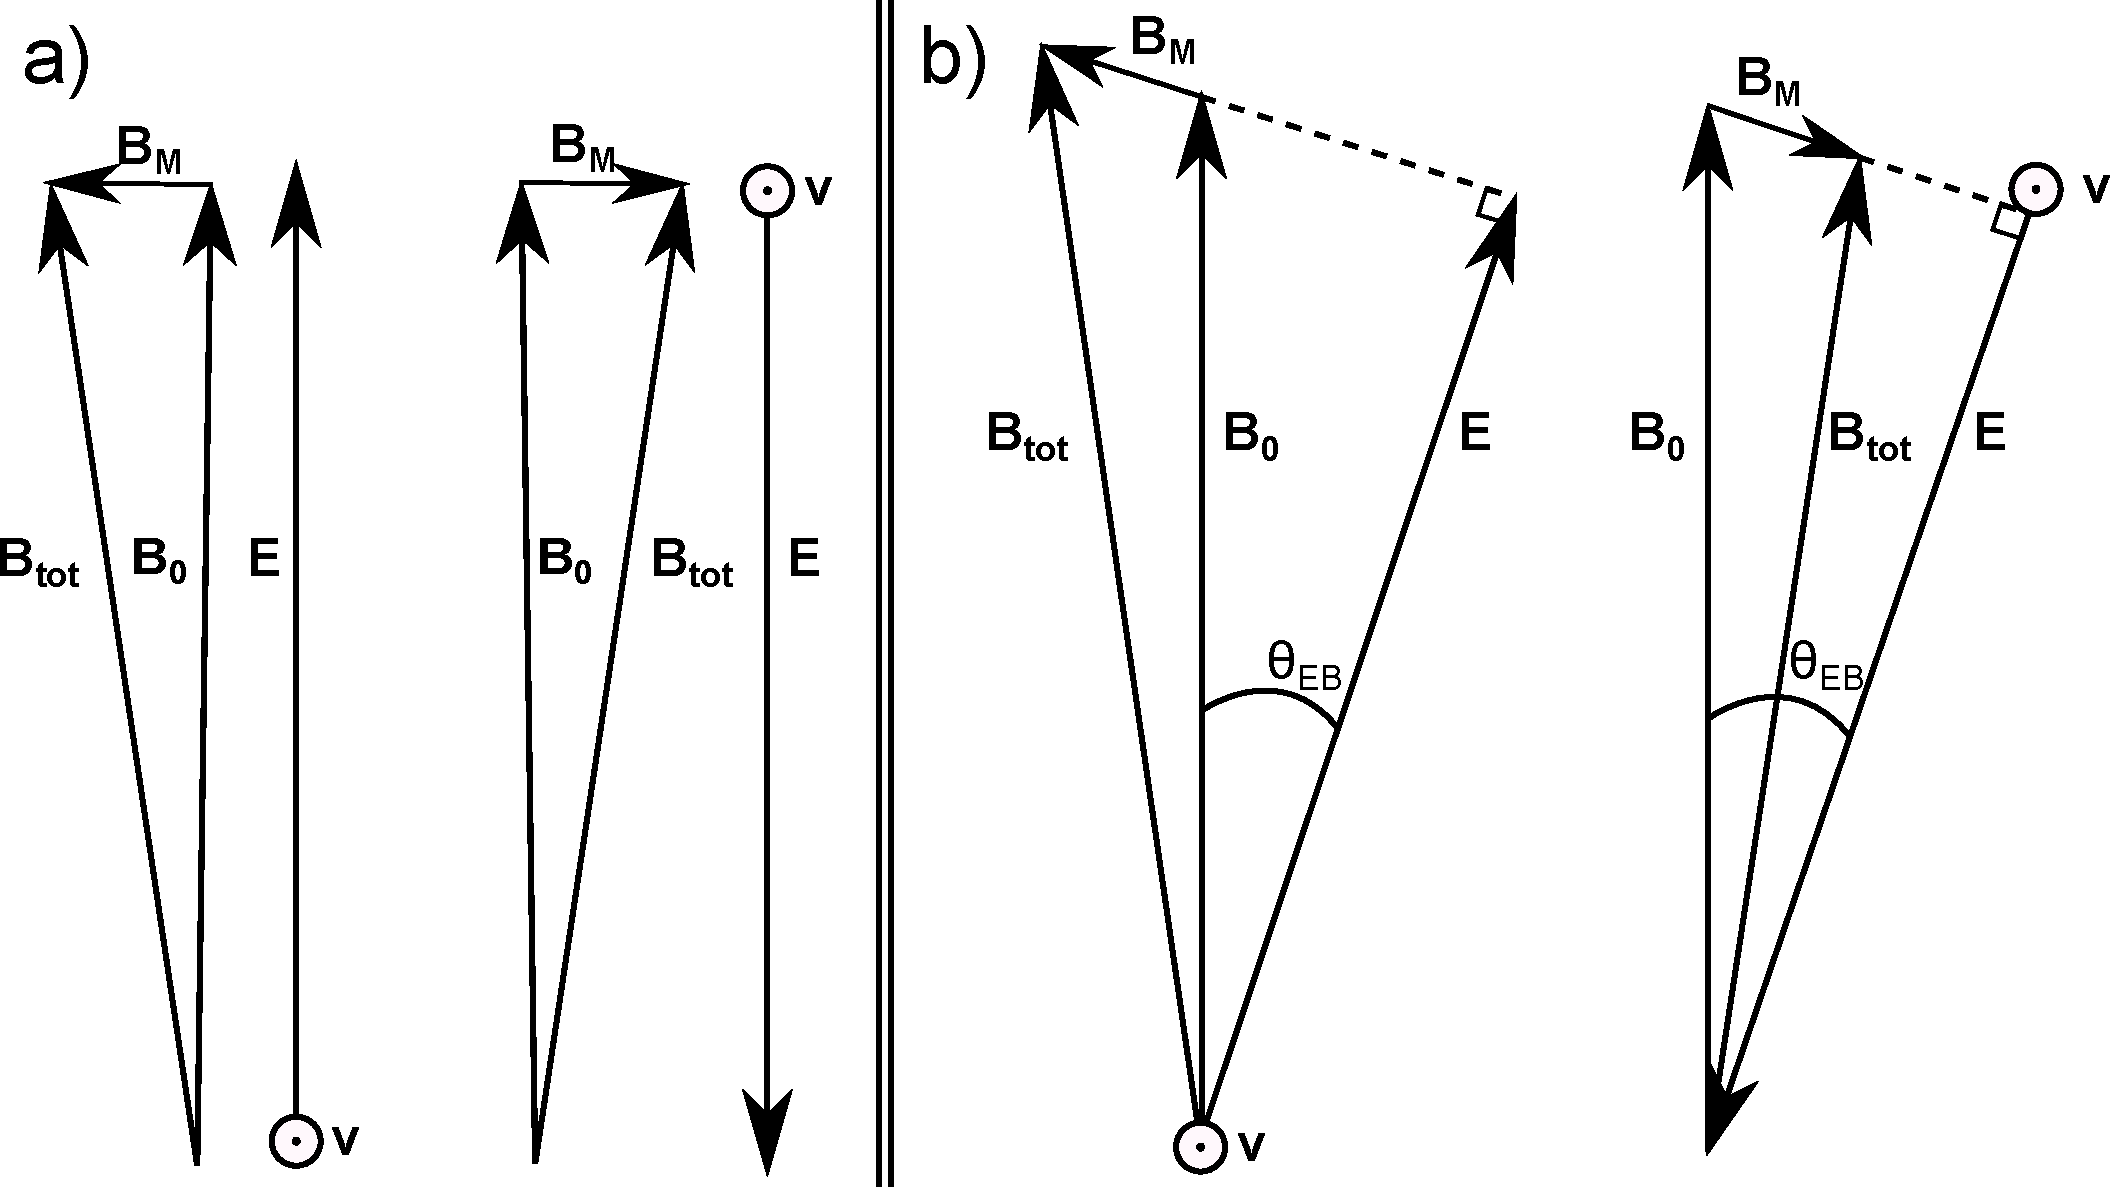
\includegraphics[scale=0.3]{Figures/Motional_Field_Diagram.pdf}
\end{center}
\caption[Diagram of motional field frequency shift]%
{\narrower Diagram of the vectors associated with a motional field frequency shift. Boosting into the rest frame of a particle with lab-frame velocity $\mathbf{v}$ partially transforms the lab-frame $\mathbf{E}$-field into an additional $\mathbf{B_M}$. a) In the limit that the fields $\mathbf{E}$ and $\mathbf{B}$ are (anti)parallel, the motional field adds quadratically to $\mathbf{B}_0$ and changes the magnitude of $\mathbf{B_{tot}}$ by the same degree for both $\mathbf{E}$-field orientations. b) If $\mathbf{E}$ and $\mathbf{B}$ are out of alignment, $\mathbf{B_M}$ acquires a component along $\mathbf{B}_0$ which adds constructively with one voltage polarity and destructively with the other.}
\label{MotionalFieldDiagram}
\end{figure}

To first order, the Hg EDM experiment is immune to such effects simply because the vapor cells are macroscopically at rest inside the apparatus. However, the distribution of polarized atoms can evolve under the de-polarizing influence of the probe beam, which undergoes absorption as it traverses the cell. Because the electric field is flipped between each pump-probe cycle, any repeated motion of the center of polarization will create a magnetic field in the rest frame of the polarized atoms which follows the high-voltage reversal. However, the vector character of the shift is such that $\mathbf{B}'$ and $\mathbf{B}_0$ add only quadratically if $\mathbf{E}$ is parallel to $\mathbf{B_0}.$ Therefore, the leading-order effect of motional magnetic fields is due to the projection of $\mathbf{B}'$ onto $\mathbf{B}_0$, proportional to the sine of the angle $\theta_{EB}$ between the electric field and $\mathbf{B_0}.$

Integrating the frequency shift $\Delta\omega = \gamma \beta E \sin\theta_{EB}/c$ with respect to time gives an expression for the accumulated phase 
\begin{equation}
\Delta \phi = \int^t_0 \Delta\omega dt' = \dfrac{\gamma E \sin\theta_{EB}}{c} \int^t_0 \beta dt' =  \dfrac{\gamma E \sin\theta_{EB}\Delta x}{c^2}
\end{equation}
which depends on the total displacement of the center of polarization $\Delta x$ \cite{2013_Hg_EDM_PRA}. Utilizing our knowledge of the magnetic field gradients inside the EDM apparatus, we can extract the displacement from the average phase shift observed in the probe phase as the center of polarization moves across a known $\partial^2 B_y/\partial y \partial x.$ Figure \ref{MotionalFieldShift} shows the result for the phase shift of the second probe period averaged over a sample of 8 days worth of data, spanning multiple sequences. From the first recorded data point, the initial phase changes by $\sim$1.2$\cdot 10^{-5}$ s$^{-1}$, which we combine with a field gradient of $2.0 \cdot 10^{-4}$ s$^{-1}$/mm for a total displacement $\Delta x = 0.06$ mm. With $\gamma = 4.844 \cdot 10^7$ s$^{-1}$/T and $E = 10^6$ V/m, the limit on the accumulated phase shift is $\Delta \phi = 3.23 \cdot 10^{-8} \sin\theta_{EB}.$ Estimating $\theta_{EB} \leq 20$ mrad and dividing the accumulated phase difference by 170 s, the limit on the frequency shift induced by motional field effects is $\Delta \omega \leq 3.8 \cdot 10^{-12}$ s$^{-1}$, which gives an EDM systematic 
\begin{equation}
\delta d_{MF} = 2.49 \cdot 10^{-31} e\cdot \text{cm}.
\end{equation}

\begin{figure}
\begin{center}
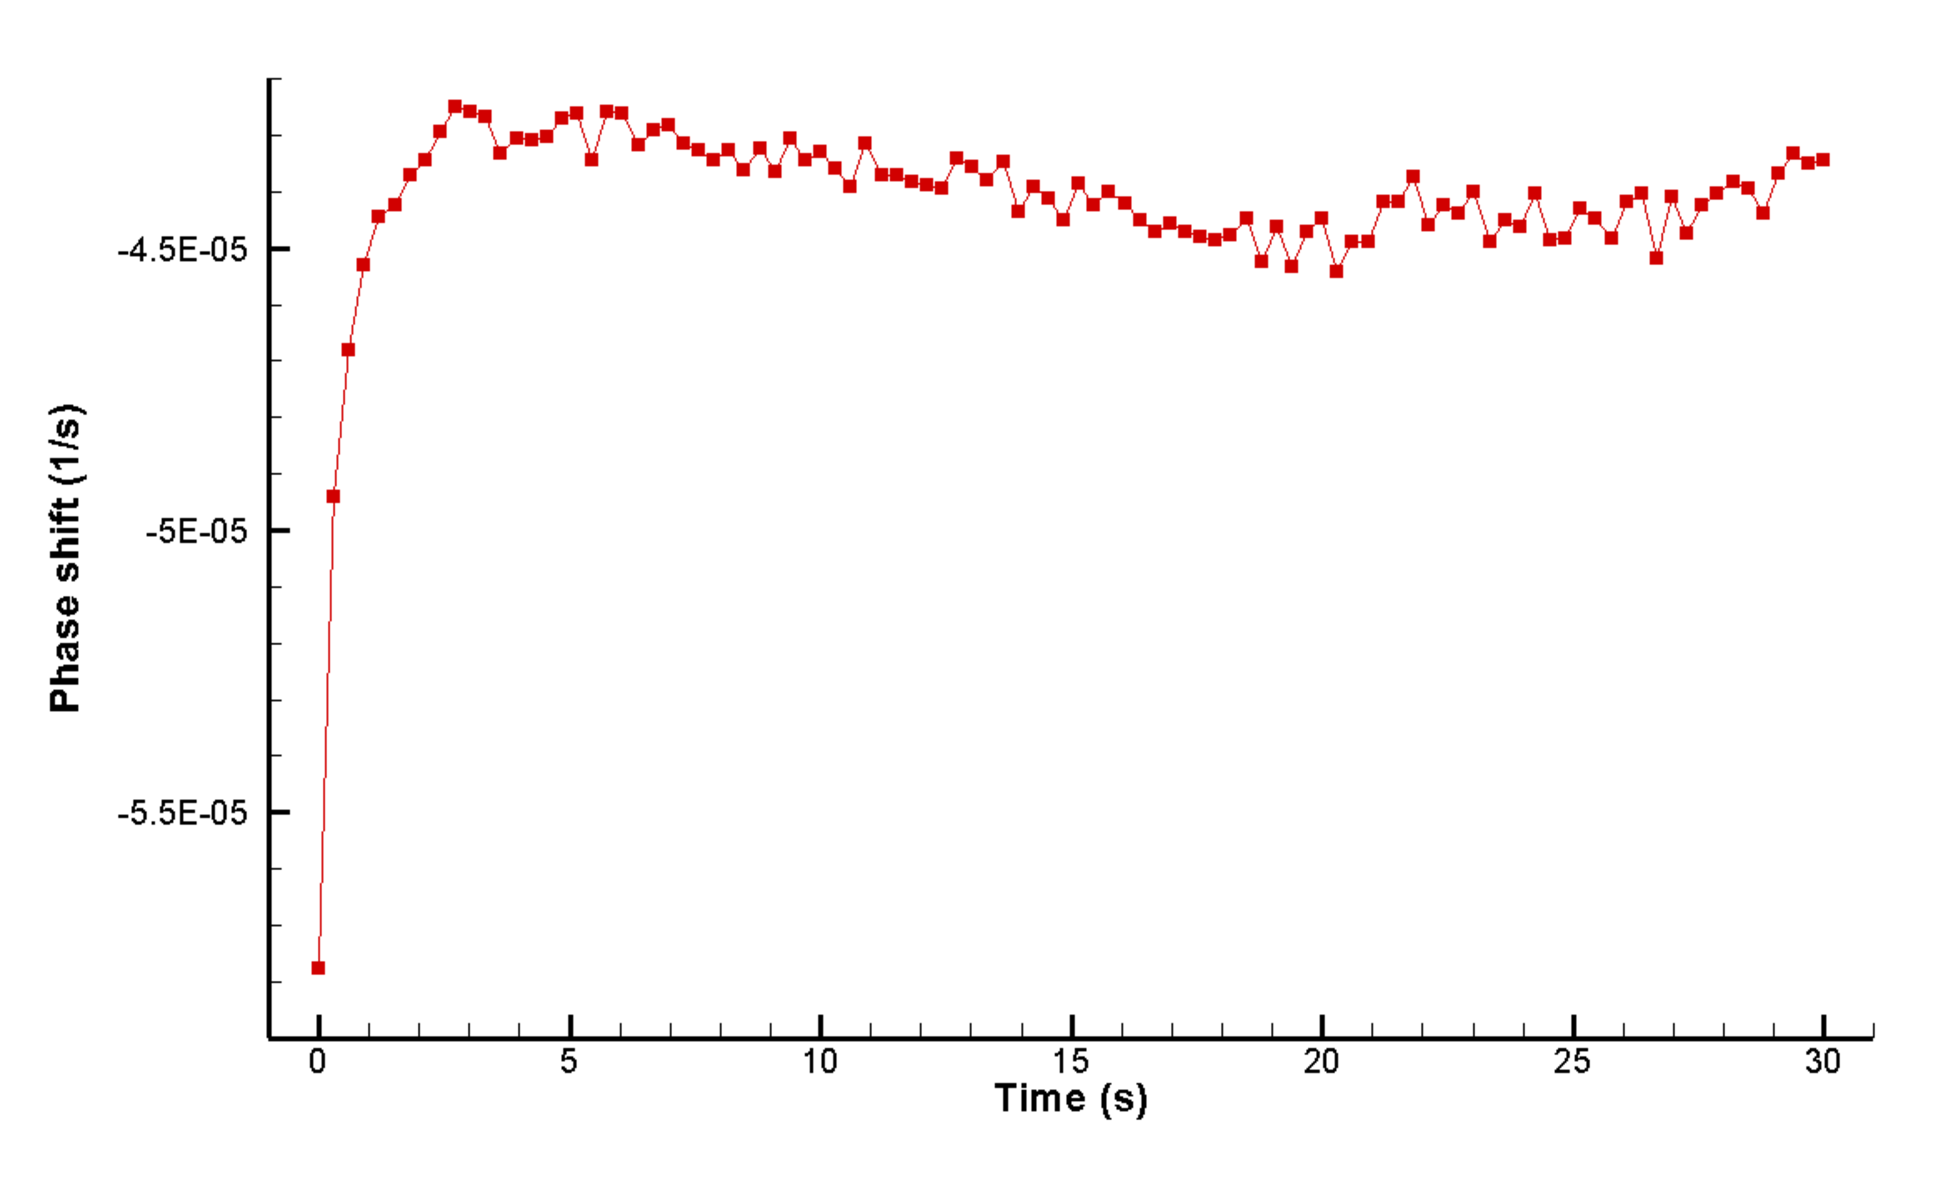
\includegraphics[scale=0.3]{Figures/Motional_Field_Phase_Shift.png}
\end{center}
\caption[Average Phase Shift $\Delta\phi_{MT_MB}(t)$]%
{\narrower The phase shift between the two middle cells for the second probe period, averaged over 8 daily runs from separate sequences ($\sim$1800 pump-probe cycles). The phase accumulated during the first 1.0 s of the probe period is consistent with a displacement of the center of polarization by 0.06 mm.}
\label{MotionalFieldShift}
\end{figure}	

\section{Charging currents}
The action of ramping the high voltage up or down causes displacement currents to flow in or out of the walls of the cell vessel and the tin-oxide coated groundplane surfaces. If these currents cause any residual magnetization of the groundplane, vessel walls, or the cells themselves, the associated magnetic field would induce a frequency shift that changes with HV reversal.\footnote{While it may be difficult to see how a change in the relatively small voltage across the cells can significantly alter their behavior, the authors of \cite{2006_ILL_nEDM} have found that changing the HV polarity (from any starting point) in the neutron EDM apparatus causes substantial drops in the Hg co-magnetometer coherence time, for unknown reasons.} To constrain the impact of charging currents, EDM data were gathered at two distinct voltage ramp rates. The slower voltage ramp would cover the full 20 kV slew in 30 seconds, or 670 V/s; the faster rate would ramp between $\pm$ 10 kV in 5 seconds, or 4 kV/s. At the slow ramp rate, the inner groundplane channels recorded an average charging current of 0.81 nA (0.80 on top, 0.82 on the bottom), and the outer channels averaged 1.89 nA (2.02 on top, 1.76 on the bottom). While the current monitors were saturated during the HV ramp at the faster rate, we can assume that the charging currents were enlarged by a factor of 6. 

To leading order, any magnetization of the apparatus is likely to affect the average magnetic field more strongly than a $\mathbf{B}$-field gradient. Therefore, we constrain the systematic effect by taking the correlation between the HV ramp rate and the average HV-correlated precession frequency of the atoms $\bar{\omega}$ while the probe light is on. Comparing the HV correlation values obtained using the two different ramp rates, we have a correlation slope of $\bar{\omega}(I_{ch}) = (7.4 \pm 15.3) \cdot 10^{-9}$ s$^{-1}$/nA. The average charging current from each side of the groundplane (inner + outer channels) is 9.46 nA. To obtain an EDM systematic estimate, we multiply the current by the correlation of $\bar{\omega}(I_{ch})$ and the correlation between $\Delta\omega_{EDM}(\bar{\omega}) = (3.07 \pm 0.77) \cdot 10^{-5}$. Our result for the charging current-induced EDM frequency shift is $(2.95 \pm 9.34) \cdot 10^{-12}$ s$^{-1}$, which gives a 1-$\sigma$ EDM systematic contribution 
\begin{equation}
\delta d_{CC} = 1.89 \cdot 10^{-31} e\cdot \text{cm}.
\end{equation}

\section{Geometric phase (Berry's phase)}
One of the most subtle systematic effects in any EDM experiment in which the particles are macroscopically at rest is the influence of \textit{geometric phase} (also known as \textit{Berry's phase}). The effect was originally discovered and analyzed in the context of an EDM experiment with an atomic beam of neutral atoms \cite{1991_Commins_Geometric_Phase}, and was treated extensively in the context of ultracold-neutron-based EDM experiments \cite{2004_Geometric_Phase_ILL_nEDM}. Motion of particles in the plane orthogonal to the applied fields $\mathbf{E}$ and $\mathbf{B}_0$ creates motional magnetic fields $\mathbf{B}_m = (\mathbf{v}\times \mathbf{E})/c^2$. If there is a non-zero gradient in the direction of $\mathbf{B}_0$, then the condition $\nabla \cdot \mathbf{B} = 0$ implies there must be some corresponding gradients in the radial direction. If specular reflections at the walls allow the particles to trace out a semi-circular `orbit' around the vessel, then the combination of motional and transverse gradient fields can create an additional magnetic field shift that is linear in $\mathbf{E}$ and differs for particles circling the vessel in opposite directions. The coupling between the observed frequency and the electric field due to geometric phase is illustrated in Figure \ref{GeometricPhase}.
\begin{figure}
\begin{center}
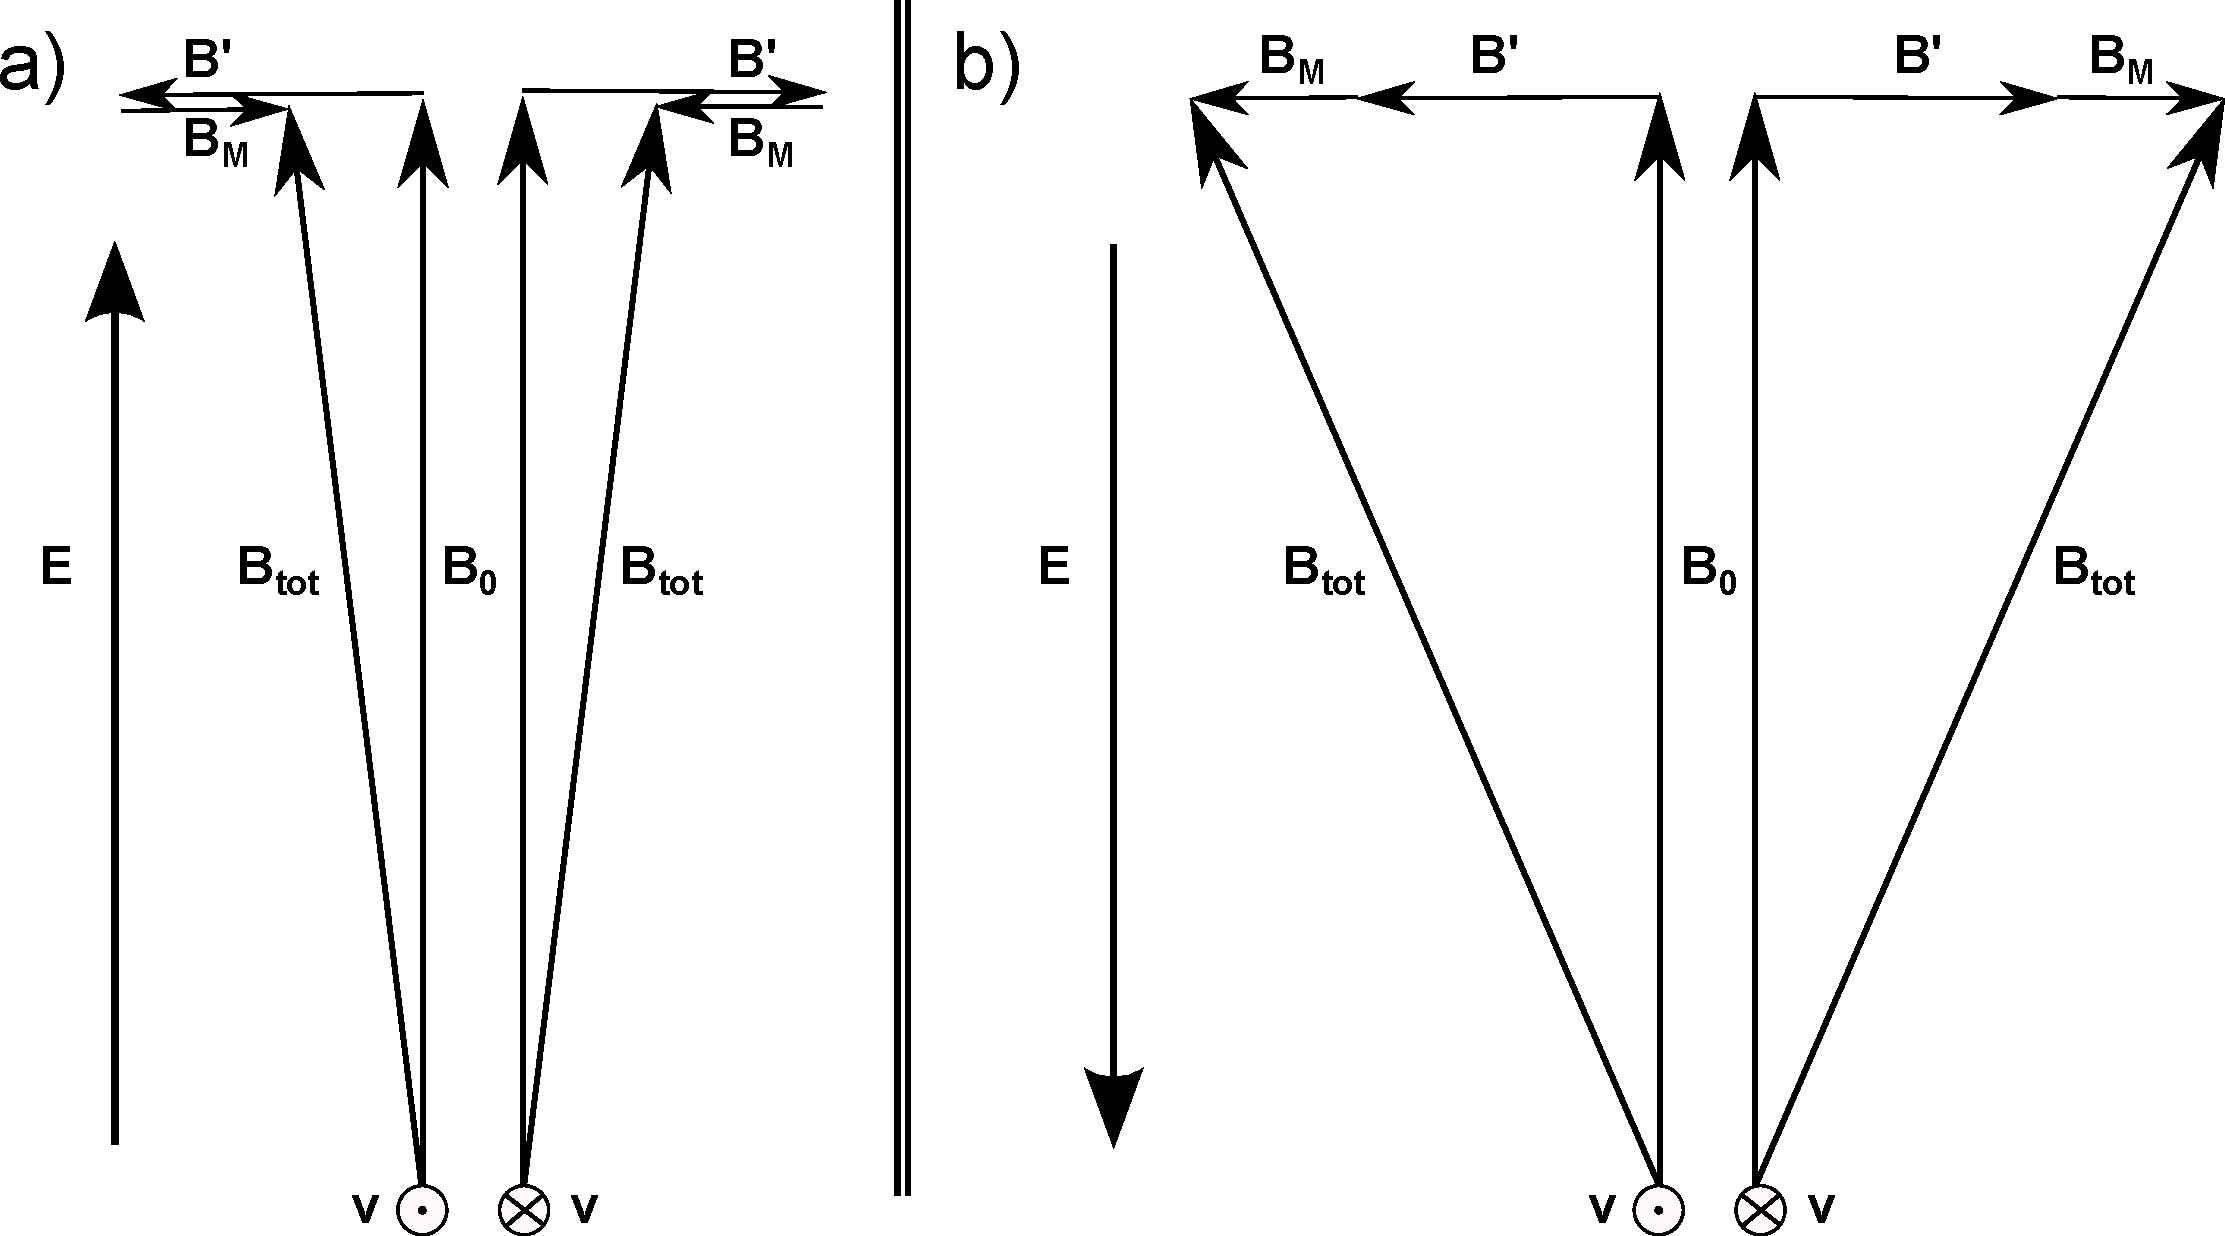
\includegraphics[scale=0.3]{Figures/Geometric_Phase.pdf}
\end{center}
\caption[Vector Diagram of Geometric Phase Shift]%
{\narrower A diagram of the fields as seen by a confined particle undergoing shallow-angle, specular reflections on the walls of a cylindrical container, moving CCW (when viewed from above) with a radial magnetic field gradient $\mathbf{B'}$. a) The fields seen on either side of the container with $\mathbf{E}$ directed up. The motional field $\mathbf{B_M}$ points radially inward, opposite the gradient field $\mathbf{B'}$, while the vector sum with $\mathbf{B}_0$ determines the measured precession frequency. b) When $\mathbf{E}$ is flipped, $\mathbf{B_M}$ points outward (assuming the particle's motion is unchanged), adding constructively to $\mathbf{B'}$ at all points on the particle's path around the rim, thus increasing the total field $\mathbf{B_{tot}}$ relative to case (a). In this manner, the combination of a vertical field gradient and a preferred CCW (or CW) motion of the particles around the container can couple the precession frequency to $\mathbf{E},$ resulting in a systematic shift of the measured EDM value.}
\label{GeometricPhase}
\end{figure}

The authors of \cite{2005_Lamoreaux_and_Golub_nEDM_geometric_phase} give an expression for the effect of geometric phase on the measured precession frequency:
\begin{equation}
\label{GPsystematic}
\delta \omega = \dfrac{R^2\gamma^2E}{2 c^2}\dfrac{\partial B_y}{\partial y} \dfrac{4}{(x_1^4- x_1^2)} \dfrac{1}{1+(\omega_0 R^2/Dx_1^2)^2}
\end{equation}	
where $R$ is the radius of the containing vessel, $D$ is the diffusion constant, $x_1 = 1.84$ is a constant for cylindrical geometry, $\gamma$ is the gyromagnetic ratio, $E$ is the electric field strength, $\partial B_y / \partial y$ is the magnetic field gradient in the direction of $\mathbf{B}_0$, and $c$ is the speed of light in vacuum.\footnote{The authors of \cite{2005_Lamoreaux_and_Golub_nEDM_geometric_phase} express the result for $\delta \omega$ in Gaussian units, subsuming a factor of $1/c$.} Using $D = 3\cdot10^{-5}$ m$^2$/s, $\gamma = 4.84\cdot 10^7$ s$^{-1}$/T, $E = 10^6$ V/m, $R = 1.15 \cdot 10^{-3}$ m, and $\partial B_y / \partial y \approx \Delta \omega / \gamma \Delta y  = 2.0 \cdot 10^{-9}$ T/m, we obtain $\delta \omega = 3.93\cdot 10^{-13}$s$^{-1}$, for an EDM systematic  
\begin{equation}
\delta d_{GP} = 6.46\cdot 10^{-33} e\cdot \text{cm}.
\end{equation} 
This limit is substantially smaller than the corresponding uncertainty of $1.0\cdot 10^{-27} e \cdot \text{cm}$ in the neutron EDM results \cite{2006_ILL_nEDM}. This is mostly due to the size of the Hg EDM cells and the presence of buffer gas. The radius of the neutron/Hg volume in \cite{2006_ILL_nEDM} is approximately 10-20 times that of the Hg EDM cells, leading to suppression of the effect in the Hg experiment by a factor of 100-400. In addition, the small diffusion constant $D$ for cells with $\sim$0.5 atm of buffer gas enhances the denominator of the final term in Eq. \ref{GPsystematic}, reducing the effect for our experiment by a factor $\approx 1/\omega_0 \approx 1/2700$ relative to the ultracold neutron experiment \cite{2006_ILL_nEDM}. The authors of \cite{2005_Lamoreaux_and_Golub_nEDM_geometric_phase} note that the effect of geometric phase may be enhanced when the orbital frequency $\omega_r$ of a particle undergoing specular reflections at some shallow angle at the vessel walls is near the Larmor frequency $\omega_0$. In the case of the Hg EDM experiment, the presence of high-pressure buffer gas causes a given atom to undergo velocity-changing collisions approximately $10^9$ times per second, severely limiting the diffusion speed and ensuring $\omega_0 \gg \omega_r$. Finally, the size of the gradients in the magnetic fields is smaller in the Hg EDM experiment than in the larger ultracold neutron apparatus. We estimate the magnetic field gradient in the vertical direction $\partial B_y / \partial y \approx \Delta \omega / \gamma \Delta y  = 2.0 \cdot 10^{-9}$ T/m, equivalent to $2.0 \cdot 10^{-7}$ G/cm.\footnote{The geometric phase effect reported in \cite{2009_Hg_EDM} was overestimated by 2 orders of magnitude due to an error in converting the frequency difference to an EDM systematic. The correct error is $1.8\cdot10^{-33} e \cdot \text{cm}$, not $1.8\cdot10^{-31} e \cdot \text{cm}$, as quoted. Similarly, the result for geometric phase in \cite{2013_Hg_EDM_PRA} is too large by one order of magnitude.} 

\section{Stark interference}
Stark interference refers to an effect on the $^1S_0 \rightarrow ^3P_1$ transition amplitude caused by application of a static electric field. The field can mix in magnetic dipole (M1) and electric quadrupole (E2) amplitudes, changing the absorption profile of the E1 transition \cite{Khriplovich_Lamoreaux}. The effect was first measured in Hg using the EDM apparatus in \cite{2011_Hg_Stark_Interference}. Denoting the atomic polarization as $\mathbf{\sigma}$ and the unit vector in the direction of the light polarization vector as $\hat{\epsilon}$, the vector dependence of the Stark interference effect is is similar for the $F=1/2 \rightarrow F=1/2$ and $F=1/2 \rightarrow F=3/2$ hyperfine components in $^{199}$Hg:
\begin{equation}
(\delta\alpha/\alpha)_{1/2} = -2(\delta\alpha/\alpha)_{3/2} = a_{SI}(\hat{\epsilon} \cdot \mathbf{E})(\hat{k} \times \mathbf{E}) \cdot \mathbf{\sigma}.
\end{equation}
In both expressions, the M1 and E2 amplitudes have been combined into a single coefficient a$_{SI}$. Comparing the $(\hat{k} \times \mathbf{E}) \cdot \mathbf{\sigma}$ vector dependence of the effect to the Hamiltonian term $\mathbf{B} \cdot \mathbf{\mu}$, the effect of Stark interference on the Larmor frequency is comparable to an effective magnetic field along $(\hat{k} \times \mathbf{E})$. If $(\hat{k} \times \mathbf{E})$ has some non-zero projection onto the applied field $\mathbf{B}_0$, The effect of Stark interference on the atomic precession frequency is linear in $\mathbf{E}$, causing it to behave like an EDM. 

\begin{table}	
\begin{center}
\caption[Systematic error budget]%
{\narrower Final estimates of systematic uncertainties on the measured EDM value.}
\label{Systematics} 
\begin{tabular}{cc}	
\hline \hline
Effect & Systematic Estimate \\
\hline	
Axial Cell Motion 						& $12.6 \cdot 10^{-31} e\cdot \text{cm}$ \\
Radial Cell Motion 						& $3.36 \cdot 10^{-31} e\cdot \text{cm}$ \\
Leakage Currents						& $5.02 \cdot 10^{-31} e\cdot \text{cm}$ \\
$\mathbf{E}^2$ Effects					& $3.04 \cdot 10^{-31} e\cdot \text{cm}$ \\
Parameter Correlations					& $2.33 \cdot 10^{-31} e\cdot \text{cm}$ \\
$\mathbf{v}\times\mathbf{E}/c$ Fields	& $2.29 \cdot 10^{-31} e\cdot \text{cm}$ \\
Charging Currents						& $1.89 \cdot 10^{-31} e\cdot \text{cm}$ \\
Geometric Phase							& $0.06 \cdot 10^{-31} e\cdot \text{cm}$ \\
\hline
\textbf{Quadrature Sum:}				& $14.78 \cdot 10^{-31} e\cdot \text{cm}$ \\
\hline \hline
\end{tabular} 
\end{center}
\end{table}

While Stark interference was included as a systematic effect in previous iterations of the experiment, it only operates while the probe light is on. Because the newest EDM result extracts the accumulated phase difference between cells while the probe light is blocked, this effect was not part of the systematic error budget presented in \cite{2016_Hg_EDM}.

\section{Final result}

\begin{figure}
\begin{center}
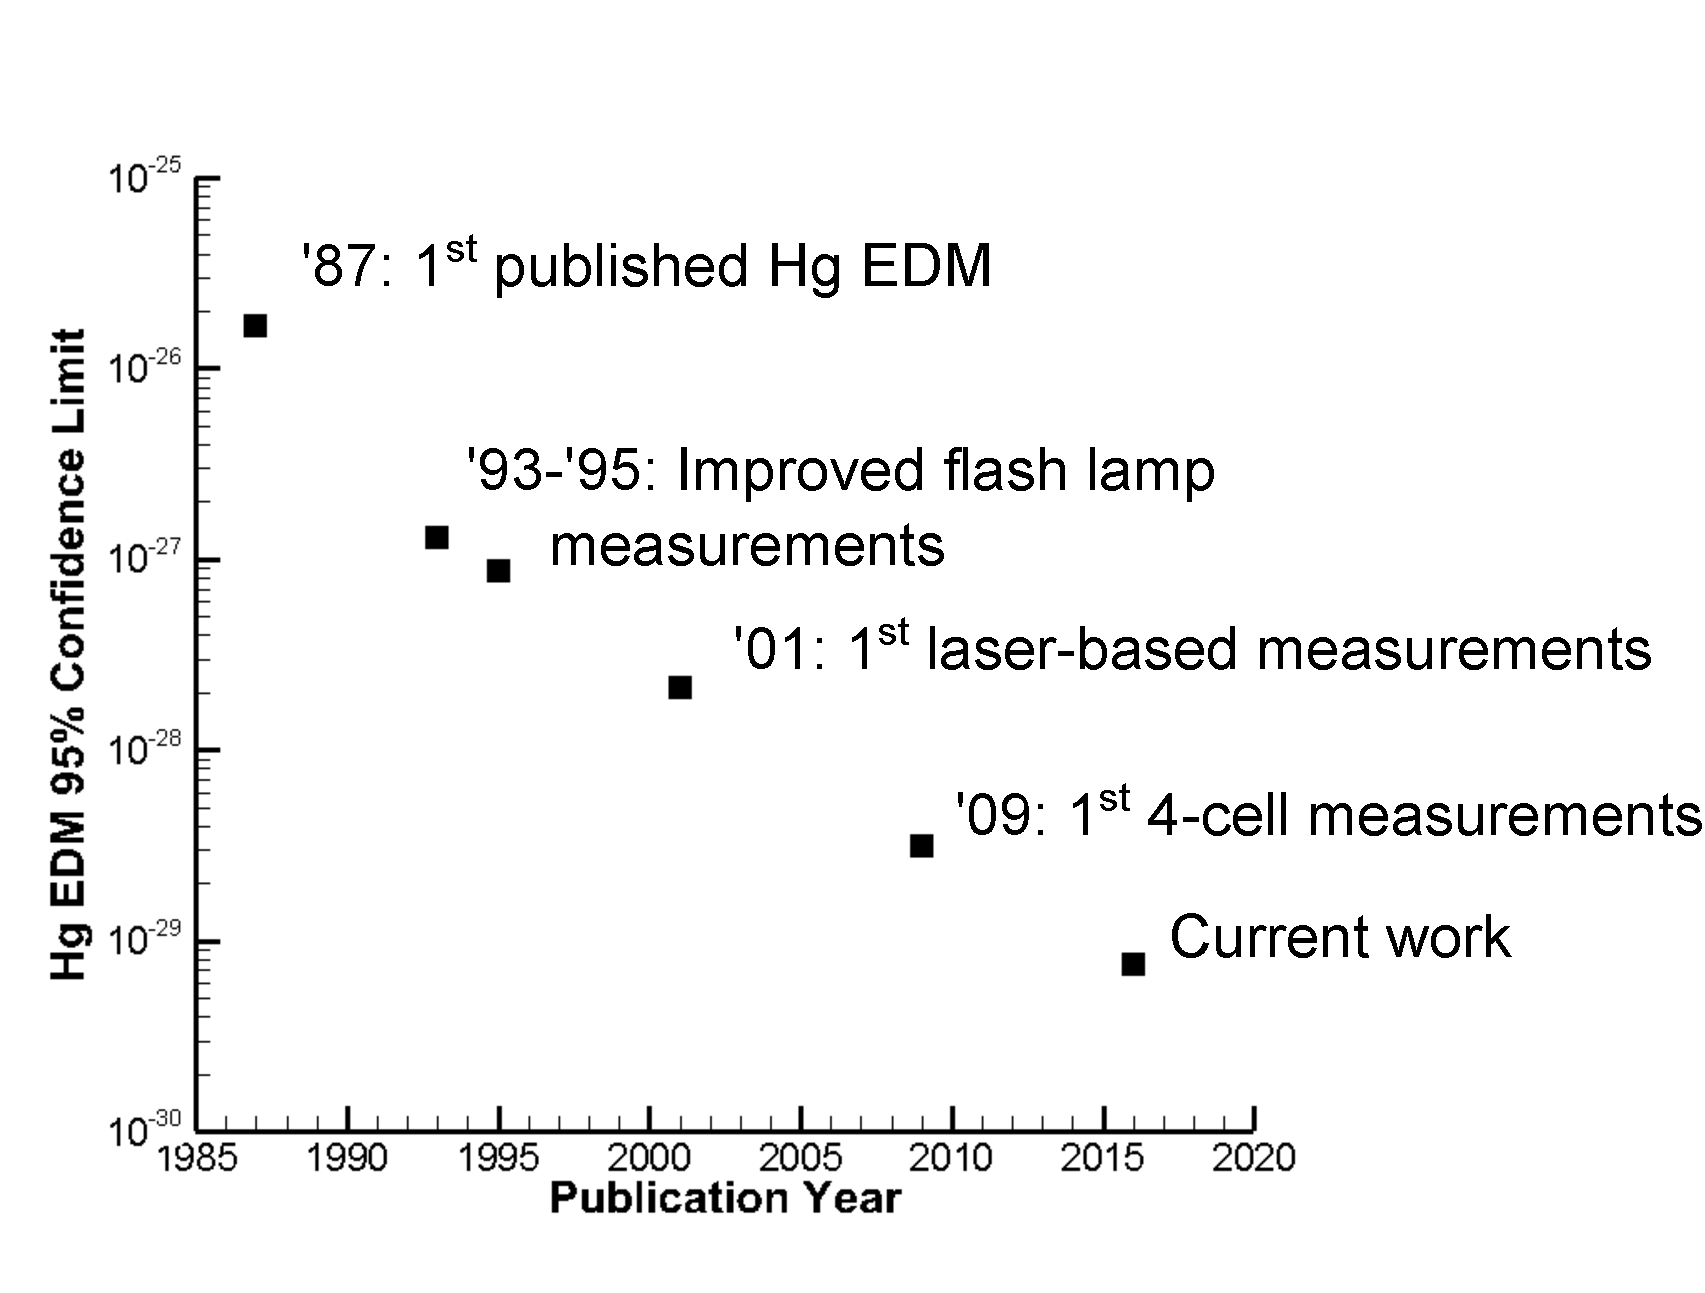
\includegraphics[scale=0.45]{Figures/Hg_EDM_Limits_vs_time.pdf}
\end{center}
\caption[$^{199}$Hg EDM limits vs. time]%
{\narrower The 95\% confidence limits established by each successive iteration of the Hg EDM experiment. Early generations of the experiment used flash lamps to pump and probe two cells with Hg atoms. The first laser-based measurements were published in 2001, and the first 4-cell results were published in 2009.}
\label{Limits_vs_time}
\end{figure}	

The combined systematic error budget for the EDM experiment is presented in Table \ref{Systematics}. When combined in quadrature with the statistical error of $2.75 \cdot 10^{-30} e \cdot \text{cm}$, the final experimental result is
\begin{equation}
d_{Hg} = (2.20 \pm 3.12) \times 10^{-30} e\cdot \text{cm}.
\end{equation}
We place a symmetric confidence limit on the magnitude of the EDM by solving 
\begin{equation}
\dfrac{1}{\sigma\sqrt{2\pi}}\int^L_{-L}e^{-(\mu-x)^2/2\sigma^2}dx\geq \alpha
\end{equation}
for the value of $L$ which satisfies the above relation for a chosen value of $\alpha$. We take $\alpha$ to be 95\%, which returns an upper limit on the $^{199}$Hg EDM
\begin{equation}
|d_{Hg}| < 7.4\times 10^{-30} e\cdot \text{cm} \text{ (95\% C.L.).}
\end{equation}
This limit is the basis for the limits on $CP$-violating quantities presented in the following chapter.

\chapter{Theoretical Interpretation of EDM Limit}	
\label{TheoryChapter}
The level of precision attained in limiting (or measuring) an EDM of the $^{199}$Hg atom is of little use for fundamental physics without the detailed knowledge of atomic, nuclear, and hadronic physics necessary to translate the results described in this thesis to meaningful constraints on theories of physics beyond the standard model. Unfortunately, the $^{199}$Hg nucleus is considered especially difficult to model, even relative to similarly massive nuclei. As such, relatively few attempts have been made by the community of theorists to calculate the physical quantities underlying the atomic EDM. Equally unfortunate is the fact that there is little agreement within the set of calculations that have been made. This chapter summarizes some of the relevant results, beginning with the transition from atomic quantities of interest to nuclear moments, and works downward to possible constraints on theories of `new physics'.

\section{Schiff moment limits from atomic physics}
The most important theoretical results are those which relate the atomic EDM to the nuclear Schiff moment, discussed in detail in Section \ref{Schiff_Moment}. The Schiff moment is the basis for limiting all the $CP$-violating nuclear observables of interest, and the upper bounds on electronic or semi-leptonic observables which can be set based on the $^{199}$Hg EDM measurement are far less rigorous than the corresponding nuclear quantities. Fortunately, the relationship between the nuclear Schiff moment and the atomic EDM is fairly well understood. Recent results of atomic structure calculations are compiled in Table \ref{SchiffMomentValues}. Despite the presence of a few outliers, there is good agreement at the 25\% level across various methods.
\begin{table}[t] 									% ht specifies location
\begin{center} 																	% used for centering table
\caption[Schiff moment contributions to $^{199}$Hg EDM]
{\narrower Calculations of the $^{199}$Hg EDM contributions from the nuclear Schiff moment $S$. Results are given for $\mathbf{d}_{Hg}$ in units of $\left(S/e \cdot  fm^3\right) e\cdot \text{cm}$.}\label{SchiffMomentValues} 
\begin{tabular}{cccc}	 														% 4 columns 
\hline \hline                													% inserts double horizontal lines 
Reference & Year  & Method & $\mathbf{d}_{Hg} \left(S/e \cdot  fm^3\right) e\cdot \text{cm}$  \\ [0.5ex]	
\hline                   														% inserts single horizontal line 
\cite{2015_Singh_and_Sahoo_Hg_Schiff_Moment}& 2015 & Coupled-cluster						&-2.1$\cdot 10^{-17}$ \\ 
\cite{2009_Latha_et_al_Hg_EDM, 2015_Latha_et_al_Hg_EDM_Correction}	& 2015 & Coupled-cluster 						&-2.5$\cdot 10^{-17}$ \\
\cite{2014_Radziute_et_al_DHF_EDM}         	& 2014 & Dirac-Hartree-Fock						&-2.5$\cdot 10^{-17}$ \\ 
\cite{2009_Dzuba_Flambaum_Porsev_EDMvSM}   	& 2009 & Dirac-Hartree-Fock						&-1.2$\cdot 10^{-17}$ \\
\cite{2009_Dzuba_Flambaum_Porsev_EDMvSM}   	& 2009 & Random Phase Approximation				&-3.0$\cdot 10^{-17}$ \\
\cite{2002_Dzuba_et._al._EDMvsSM} 		  	& 2002 & Averaged \textit{ab initio} results	&-2.8$\cdot 10^{-17}$ \\
\hline
\textbf{Average:}							&	   &								&$\mathbf{-2.4\cdot 10^{-17}}$\\
\hline 
\hline																			% inserts single line 
\end{tabular}  
\end{center}
													% used to refer to this table 
\end{table}	
	
\section{Schiff moment parameterization from nuclear physics}
The next step in interpreting the limits on an EDM in $^{199}$Hg is to calculate the Schiff moment from nuclear theory. The Schiff moment is typically parameterized in terms of a set of pion-nucleon-nucleon ($\pi NN$) coupling constants $\bar{g}_{(i)}$:
\begin{equation}
S = (a_0 + b) g\bar{g_0} + a_1 g\bar{g_1} + (a_2 - b)g\bar{g_2}
\end{equation}	 
where $g$ is an overall interaction strength parameter, and $g\bar{g_0}, g\bar{g_1}, g\bar{g_2}$ represent the $P$-odd, $T$-odd isoscalar, isovector, and isotensor $\pi NN$ couplings, respectively. The coefficients $a_i$ describe the dependence of the Schiff moment on a $P$-odd, $T$-odd part of the nuclear potential, while $b$ parameterizes the dependence on the nucleon EDMs \cite{2010_Engel_self-consistent_Schiff_moments}. Note that not all authors include values for $b$ in the calculations; the contribution from the nucleon EDMs is expected to be small relative to the Schiff moment, and the ratio of $b$ to $a_{0,2}$ is typically found to be 1/3 or less in calculations which take this into account.

Unfortunately, calculations of the nuclear Schiff moment in terms of the $\bar{g}_{\pi NN}^{(i)}$ are highly divergent. To date, even possible corrections to the definition of the Schiff moment remain controversial \cite{2007_Liu_et._al._Schiff_Theorem_and_Corrections, 2008_Schiff_Theorem_Rederivation}. A list of parameter calculation results (where $b=0$) was compiled in \cite{2013_Engel_et_al_EDM_review}; the data and references are reproduced in Table \ref{piNN} below. To set limits on $\bar{g}_{0,1,2}$, we use the quoted best values for $^{199}$Hg from the recent review \cite{2013_Engel_et_al_EDM_review}.\footnote{Note that the calculation has a sign ambiguity for the value of $\bar{g}_1$.} Using these values for the Shiff moment dependence, we have
\begin{equation}
|\bar{g}_0| \leq 2.3\cdot 10^{-12}, 
\end{equation}
\begin{equation}
|\bar{g}_1| \leq 1.1\cdot 10^{-12},
\end{equation}
\begin{equation}
|\bar{g}_2| \leq 1.1\cdot 10^{-12}. 
\end{equation}

\section{Nucleon EDMs}
Given the considerable uncertainty surrounding the Schiff moment of $^{199}$Hg in terms of possible $P$-odd, $T$-odd interactions between nuclei, any attempt to disregard the relevant nuclear physics and set a limit on $\mathbf{d}_{p,n}$ directly from the experimental limits on $\mathbf{d}_{atom}$ should be taken with a grain of salt. However, we may obtain limits on the nucleon EDMs $\mathbf{d}_{n,p}$ from the associated contributions to the Schiff moment from an RPA calculation with core-polarization \cite{2003_Dmitriev_and_Sen'kov_Hg_Schiff_Moment}. The proton contribution to the Schiff moment of $^{199}$Hg is relatively small because the un-paired valence nucleon in $^{199}$Hg (with $Z=80$) is a neutron. Using the result of \cite{2003_Dmitriev_and_Sen'kov_Hg_Schiff_Moment} $\mathbf{S}_{Hg} = (1.9 \cdot \mathbf{d}_n + 0.2 \cdot \mathbf{d}_p) \text{fm}^2$, we find
\begin{equation} \label{d_n}
|\mathbf{d}_n| < 1.6\cdot 10^{-26} e\cdot\text{cm} 
\end{equation}
\begin{equation} \label{d_p}
|\mathbf{d}_p| < 2.0\cdot 10^{-25} e\cdot\text{cm}. 
\end{equation}
There is an additional 30\% uncertainty in the calculation of the $\mathbf{d}_p$ contribution which is reflected in \ref{d_p}. In principle, the result for $\mathbf{d}_n$ we extrapolate from the $^{199}$Hg EDM limit supercedes the direct neutron precession experiment \cite{2015_ILL_nEDM_gravity_correction} as the world's best neutron EDM limit.

\begin{table}[t]  																
\begin{center} 																	
\caption[$\pi NN$ couplings parameterizing the Schiff moment]
{\narrower The results of several calculations of the $\pi NN$ coupling constant coefficients which can contribute to a nonzero Schiff moment in $^{199}$Hg. Note that the group of Engel \textit{et. al.} utilizes a diffferent sign convention for $\bar{g_0}, \bar{g_1}$ from other groups; the sign used in this table is consistent with \cite{2013_Engel_et_al_EDM_review}. RPA: random phase approximation, MFT: mean field theory CP: core polarization} \label{piNN}
\begin{tabular}{cccccc}															% 6 columns
\hline \hline                													% inserts double line 
Reference & Year  & Method & $a_0$ & $a_1$ & $a_2$  \\ [0.5ex]					% inserts table heading
\hline  
\cite{2010_Engel_self-consistent_Schiff_moments} & 2010 & Odd-A Skyrme MFT & 0.009 - 0.041 & -0.027 - +0.005 & 0.009 - 0.024\\ 
\cite{2005_de_Jesus_and_Engel_Hg_Schiff_Moment} & 2005 & Skyrme Quasi-RPA & 0.002 - 0.010 & 0.057 - 0.090 & 0.011 - 0.025\\  
\cite{2005_Dmitriev_et._al._Core_Polarization_in_NSM} & 2005 & RPA+CP & 0.00004 & 0.055 & 0.009\\       \cite{2005_Dmitriev_et._al._Core_Polarization_in_NSM} & 2005 & RPA & 0.09 & 0.09 & 0.18\\
\hline
\hline 																			% inserts single line 
\end{tabular} 
\end{center} 														 
\end{table}	 

\begin{figure}[p] 
\begin{center}
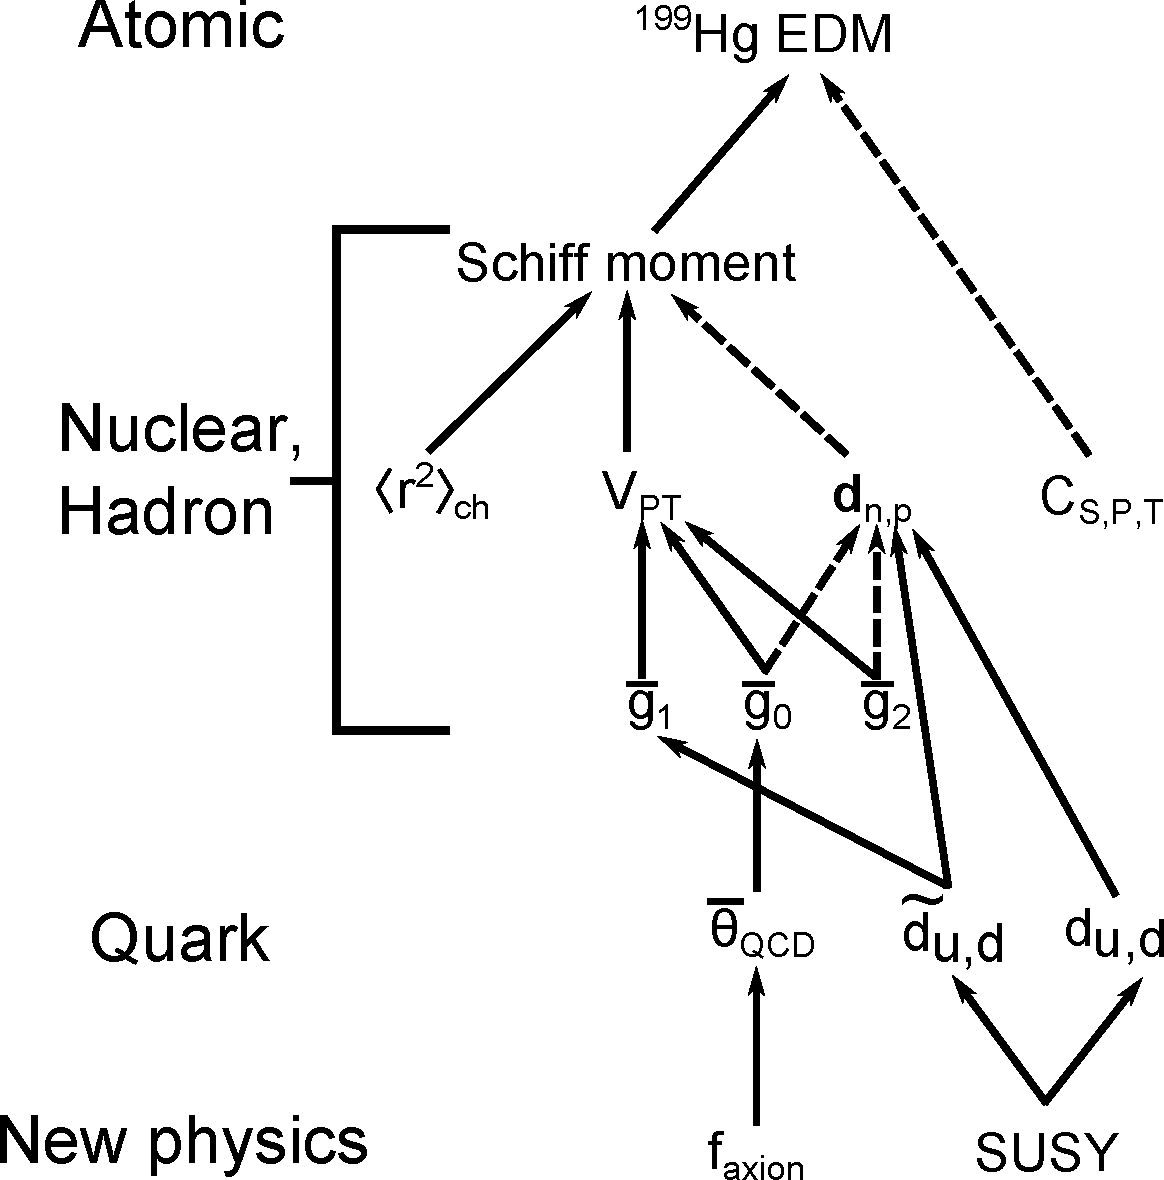
\includegraphics[scale=0.6]{Figures/Theory_Diagram.pdf}
\end{center}
\caption[EDM dependence on hadron EDMs, nuclear couplings, and fundamental physics]
{\narrower A diagrammatic view of the interrelated observables and theoretical coupling constants describing the EDM of the $^{199}$Hg atom. At each level, couplings which are expected to be below leading-order are indicated by dashed lines. The atomic EDM is primarily dependent on the Schiff moment, which depends on the size of the nuclear charge distribution $\langle r^2 \rangle _{ch}$, a $P,T$-odd piece of the nuclear Hamiltonian V$_{P,T}$, and the nucleon EDMs $\mathbf{d}_{n,p}$. $P,T$-odd electron-nucleon coupling constants $C_{S,P,T}$ may also induce an EDM; in Hg, the tensor component $C_T$ is expected to be dominant. The $P,T$-odd $\pi NN$ coupling constants $\bar{g_i}$ parameterize the nuclear interactions in terms of isoscalar ($\bar{g_0}$), isovector ($\bar{g_1}$), and isotensor ($\bar{g_2}$) components. ($\bar{g_1}$) has been calculated in terms of quark EDMs $d_{u,d}$ and quark-chromo EDMs $\tilde{d}_{u,d}$, as has the EDM of the neutron. In addition, the pseudoscalar coupling constant ($\bar{g_0}$) can be related to the CP violating term in the QCD Lagrangian, which is dependent on the nature of the axion field in Peccei-Quinn theory \cite{1977_Peccei_Quinn}. Additional contributions to an atomic EDM may come from the magnetic quadrupole or electric octupole moments, but the spin of $^{199}$Hg is too small to possess either one. A possible electron EDM may also contribute to an atomic EDM, but in Hg the electron screening makes the contribution almost negligible \cite{2004_Ginges_Flambaum_Fund._Symmetries_in_Atoms}, so it is omitted from the diagram.} \label{TheoryDiagram}
\end{figure}
 
\section{Limits on QCD parameters} 
Moving below the hadronic level of Figure \ref{TheoryDiagram}, nuclear and nucleon EDMs can be generated from $\bar{\theta}_{QCD}$, the Weinberg 3-gluon operator, or the EDMs or chromo-EDMs of the constituent quarks. Mathematically, we have a $CP$-violating Lagrangian \cite{2002_Pospelov_quark_chromo_EDM}
\begin{equation} \label{CPV_Lagrangian}
\mathcal{L}^{CPV} = \dfrac{g_s^2}{32\pi^2} \bar{\theta}_{QCD} G^a_{\mu\nu} \widetilde{G}^{\mu\nu,a} + \dfrac{1}{3}w f^{abc} G^a_{\mu\nu} \widetilde{G}^{\nu\beta,b} G_{\beta}^{\mu,c} -\dfrac{i}{2} \sum_{i=e,u,d,s} d_i \bar{\psi_i} (F \cdot\sigma) \gamma_5 \psi_i - \dfrac{i}{2} \sum_{i=u,d,s} \widetilde{d}_i  \bar{\psi_i} (G \cdot\sigma) \gamma_5 \psi_i
\end{equation} 
where $G$ represents the gluon field, $F$ is the photon field, $d$ is the EDM of an electron or quark, and $\widetilde{d}$ is the quark chromo-EDM (up, down, or strange). A quark chromo-EDM thus differs from a `conventional' EDM in that it results from a coupling of quarks to the gluon field instead of the photon field. Restricting our attention to nuclear interactions alone, the Weinberg three-gluon operator $G\widetilde{G}G$ contribution is small enough to be neglected , leaving only contributions from $\bar{\theta}_{QCD}$ and the possible quark chromo EDMs \cite{2002_Pospelov_quark_chromo_EDM}.

\subsection{$\bar{\theta}_{QCD}$}
We can set a limit on the $CP$-violating parameter in the QCD Lagrangian proportional to $\bar{\theta}_{QCD}$ using the relation $|\bar{g}_0| = 15.5\cdot 10^{-3}|\bar{\theta}_{QCD}|$. obtained independently by \cite{2015_deVries_Mereghetti_Walker_CP_violation_in_CPT} and \cite{2015_Bsaisou_et_al_Nucleon_EDMs_in_chiral_EFT}. When combined with our EDM limit, we find
\begin{equation} 
|\bar{\theta}_{QCD}| < 1.5\cdot 10^{-10}.
\end{equation}
Alternatively, we may consider lattice calculations of the neutron EDM dependence on $\bar{\theta}_{QCD}$, which seem to offer the possibility of a tighter bound. According to the results of \cite{2015_Guo_et_al_nEDM_from_lattice_QCD}, $\mathbf{d}_n = -3.9\cdot 10^{-3}|\bar{\theta}_{QCD}|$. Combining this result with the neutron EDM limit inferred in in Eq. \ref{d_n}, we obtain  
\begin{equation}
|\bar{\theta}_{QCD}| < 4.2\cdot 10^{-11},
\end{equation}
which represents nearly a factor of four reduction in the upper limit. However, since the authors of \cite{2015_Guo_et_al_nEDM_from_lattice_QCD} note that their work is to be considered ``exploratory'' rather than comprehensive, the less stringent bound of $1.5\cdot 10^{-10}$ appears more reliable for the time being.

\subsection{Quark chromo-EDMs}
In many models of new physics, the Peccei-Quinn mechanism forces $\bar{\theta}_{QCD} = 0$. In this case, the primary cause of $CP$-violating nuclear interactions is the chromo-EDMs of the quarks constituting the nucleus. An estimate was obtained in \cite{2002_Pospelov_quark_chromo_EDM} for the dependence of the isovector $\pi NN$ coupling constant $\bar{g}_{i}$ on the chromo-EDM of a linear combination of up and down quarks $\bar{g}_1=2\cdot10^{-14}\text{cm}^{-1}(\widetilde{d}_u-\widetilde{d}_d)$. Combining this with our limit on $\bar{g}_1$, we have
\begin{equation}
|(\widetilde{d}_u-\widetilde{d}_d)| < 5.7 \cdot 10^{-27} \text{cm}.
\end{equation}

Again, one could assume that one and only one quark has a non-zero chromo-EDM to obtain an `independent' limit on each quark flavor. 

\section{Limits on semi-leptonic interactions}
\begin{table}[t] 																% t = page top
\begin{center} 																	% used for centering table
\caption[Semi-leptonic tensor interaction contributions to the $^{199}$Hg EDM]
{\narrower Calculations of the atomic EDM $\mathbf{d}_{Hg}$ in units of C$_T$ $\langle\sigma_N\rangle$ e$\cdot \text{cm}$. C$_T$ is the coefficient of the tensor part of the hypothetical $P,T$-odd electron-nucleon interaction, $\langle\sigma_N\rangle$ is the magnitude of the nuclear spin vector. In the simple nuclear shell model, $\langle\sigma_N\rangle = -1/3$ \cite{2004_Ginges_Flambaum_Fund._Symmetries_in_Atoms}.}\label{C_Table} 	
\begin{tabular}{cccc}		 													% centered columns (4 columns)
\hline \hline                													% inserts horizontal lines 
Reference & Year  & Method & $\mathbf{d}_{Hg} (\text{C}_T\langle\sigma_N\rangle) \text{e}\cdot \text{cm}$  \\ [0.5ex]	
\hline 
\cite{2015_Singh_and_Sahoo_Hg_Schiff_Moment}	& 2015 & Coupled-cluster			& $-4.44\cdot 10^{-20}$ \\
\cite{2014_Radziute_et_al_DHF_EDM}				& 2014 & Multiconfiguration DHF 	& $-5.53\cdot 10^{-20}$ \\
\cite{2009_Dzuba_Flambaum_Porsev_EDMvSM}		& 2009 & Dirac-Hartree-Fock (DHF)	& $-2.4 \cdot 10^{-20}$ \\
\cite{2009_Dzuba_Flambaum_Porsev_EDMvSM}		& 2009 & Random Phase Approximation	& $-5.9 \cdot 10^{-20}$ \\
\cite{2009_Latha_et_al_Hg_EDM}					& 2009 & Coupled-cluster			& $-4.3 \cdot 10^{-20}$ \\
\cite{2008_Latha_et_al_Core_Polarization_EDM}	& 2008 & Coupled-perturbed HF		& $-6.75\cdot 10^{-20}$ \\
\cite{Khriplovich_Lamoreaux}					& 1997 & Analytical Calc.			& $-4.9 \cdot 10^{-20}$ \\ 
\cite{1985_Martensson_C_T_calc}					& 1985 & Dirac-Hartree-Fock	(DHF)	& $-2.0 \cdot 10^{-20}$ \\
\cite{1985_Martensson_C_T_calc}					& 1985 & Random Phase Approximation	& $-6.0 \cdot 10^{-20}$ \\
\hline
\textbf{Average:}								&	   &							&$\mathbf{-4.69\cdot 10^{-20}}$\\
\hline 
\hline																			% inserts single line 
\end{tabular} 
\end{center}														 
\end{table}	

Our result can also be used to place limits on $P,T$-odd scalar, pseudoscalar, and tensor electron-nucleon interactions (described by $C_S$, $C_P$, and $C_T$) which may induce an atomic EDM independent of the Schiff moment. In $^{199}$Hg the tensor interaction is expected to dominate. Many recent calculations of the tensor coefficient $C_T$ have been performed; the results are given in Table \ref{C_Table}. Using the average value of $\mathbf{d}_{Hg} = -4.69 \cdot 10^{-20} C_T \langle\sigma_N\rangle e\cdot \text{cm}$, we get a limit 
\begin{equation}
|C_T| < 1.5\cdot 10^{-10}. 
\end{equation}
Less-stringent bounds can be obtained for $C_S$ and $C_P$ using the results of \cite{2004_Ginges_Flambaum_Fund._Symmetries_in_Atoms}:
\begin{equation}
|C_S| < 1.3 \cdot 10^{-8}. 
\end{equation}
\begin{equation}
|C_P| < 1.2 \cdot 10^{-7}.
\end{equation}

\section{Electron EDM}
While it is possible to generate an atomic EDM from an EDM of the electron via the hyperfine interaction between the electron and nuclear spins, the lack of an unpaired electron spin in $^{199}Hg$ suppresses the resulting observed EDM relative to atoms or molecules with nonzero net electron spins such as Tl \cite{2002_Tl_EDM}, YbF \cite{2011_YbF_EDM}, or ThO \cite{2014_ACME_eEDM}. Because EDM experiments have been carried out with all the above systems (among others), the results of the $^{199}Hg$ EDM experiment are not particularly useful for setting an electron EDM limit. 

For the sake of completeness, we may obtain an estimate using the relation $\mathbf{d}_{Hg} = 0.012\cdot\mathbf{d}_e$ \cite{1987_Martensson_Oster_eEDM}. The result is
\begin{equation}
|\mathbf{d}_e| \leq 6.17 \cdot 10^{-28} e\cdot\text{cm (95\% C.L.)}.
\end{equation}
However, another calculation \cite{1985_Flambaum_Khriplovich_eEDM_bound} suggests the electron EDM has the opposite sign: $\mathbf{d}_{Hg} = -0.014 \cdot\mathbf{d}_e$, creating additional uncertainty about the usefulness of the $^{199}$Hg electron EDM bound. For comparison, the leading electron EDM upper bound was measured in \cite{2014_ACME_eEDM}, which obtained
\begin{equation}
|\mathbf{d}_e| \leq 8.7 \cdot 10^{-29} e\cdot\text{cm (90\% C.L.)},
\end{equation}
nearly an order of magnitude lower than our limit.

\section{Conclusion}
\begin{table}[t] 														% t = 'top'
\begin{center} 
\caption[Limits on $CP$-violating observables] 
{\narrower Limits on various $CP$-violating observables derived from the $^{199}$Hg EDM limit. Each limit is based on the assumption that it is the sole contribution to the atomic EDM.}\label{Limits}
\begin{tabular}{cccc}													% 4 columns 
\hline \hline	 														% inserts double horizontal lines 
Quantity & Expression & Limit & Ref. \\ 								% table header
\hline 																	% horizontal line underneath header
$\mathbf{d}_n$	& $\mathbf{S}_{Hg}/(1.9 \text{ fm}^2)$ 		& $1.6\cdot 10^{-26}$ $e\cdot\text{cm}$ & \cite{2003_Dmitriev_and_Sen'kov_Hg_Schiff_Moment}\\
$\mathbf{d}_p$	& $1.3\cdot\mathbf{S}_{Hg}/(0.2 \text{ fm}^2)$	& $2.0\cdot 10^{-25}$ $e\cdot\text{cm}$ & \cite{2003_Dmitriev_and_Sen'kov_Hg_Schiff_Moment}\\
$\mathbf{d}_e$	& $\mathbf{d}_{Hg}/0.012$ & $6.17 \cdot 10^{-28}$ $e\cdot\text{cm}$ & \cite{1987_Martensson_Oster_eEDM}\\
$\bar{g}_0$ 	& $\mathbf{S}_{Hg}/(0.135$ $e\cdot\text{fm}^3)$ & $2.3\cdot 10^{-12}$ & \cite{2013_Engel_et_al_EDM_review}\\
$\bar{g}_1$ 	& $\mathbf{S}_{Hg}/(0.27$ $e\cdot\text{fm}^3)$ 	& $1.1\cdot 10^{-12}$ & \cite{2013_Engel_et_al_EDM_review}\\
$\bar{g}_2$ 	& $\mathbf{S}_{Hg}/(0.27$ $e\cdot\text{fm}^3)$ 	& $1.1\cdot 10^{-12}$ & \cite{2013_Engel_et_al_EDM_review}\\
$\bar{\theta}_{QCD}$ 	& $\bar{g}_0/0.0155$ 					& $1.5\cdot 10^{-10}$ & \cite{2015_deVries_Mereghetti_Walker_CP_violation_in_CPT, 2015_Bsaisou_et_al_Nucleon_EDMs_in_chiral_EFT}\\
$(\widetilde{d}_u-\widetilde{d}_d)$ & $\bar{g}_1/(2\cdot10^{14} \text{cm}^{-1})$ & $5.7\cdot 10^{-27} \text{ cm}$& \cite{2002_Pospelov_quark_chromo_EDM}\\
$C_S$ 			& $\mathbf{d}_{Hg}/(5.9 \cdot10^{-22}$ $e\cdot\text{cm})$ & $1.3\cdot 10^{-8}$ & \cite{2004_Ginges_Flambaum_Fund._Symmetries_in_Atoms}\\
$C_P$			& $\mathbf{d}_{Hg}/(6.0\cdot10^{-23}$ $e\cdot\text{cm)}$ & $1.2\cdot 10^{-7}$ & \cite{2004_Ginges_Flambaum_Fund._Symmetries_in_Atoms}\\
$C_T$			& $\mathbf{d}_{Hg}/(4.89 \cdot10^{-20}$ $e\cdot\text{cm})$ & $1.5\cdot 10^{-10}$ & see text\\
\hline \hline															% inserts double horizontal lines				
\end{tabular} 
\end{center}
\end{table}

The results presented in this chapter are summarized in Table \ref{Limits}. On a final note, it is worth pointing out that $^{199}$Hg retains the most stringent limit on the EDM of any physical system. The authors of \cite{2015_Chupp_Xe_EDM_Motivation} performed a global analysis of EDM limits from the various possible sources of $CP$-violating interactions, attempting to constrain them using a variety of EDM results from bare neutrons, $^{199}$Hg, $^{129}$Xe, $^{225}$Ra, ThO, Cs, Tl, YbF, and TlF. They concluded that the theoretical understanding of the $^{199}$Hg Schiff moment is too poor to fully take advantage of the experimental EDM limit presented in \cite{2009_Hg_EDM}. Since our result improves the experimental limits from \cite{2009_Hg_EDM} yet further, there is reason to hope that the theoretical community will become more motivated to leverage this exceptional experimental sensitivity to improve limits on $CP$-violating parameters by making more sophisticated and reliable calculations.

\bibliographystyle{alpha}
\bibliography{Graner_EDM_Thesis}	

\appendix

\chapter{Cell Motion in an n-th order field gradient} \label{nth_gradient}
Consider a vertical gradient in $\mathbf{B}$ which goes as $y^n$: $B(y) = B_0 + B'y^n$. For some vertical translation $\delta y$, the gradient field at the center of the middle top (MT) cell is
\begin{equation}
B'_{MT}(h+\delta y) \approx B' h^n(1+n\frac{\delta y}{h})
\end{equation}
where $h$ is one half of the height of a cell (i.e., the approximate distance from the groundplane center to the center of an inner cell), and $\delta y$ is assumed to be much smaller than $h$. Similarly, for the middle bottom (MB) cell,
\begin{equation}
B'_{MB}(-h+\delta y) \approx B'(-h)^n(1-n\frac{\delta y}{h})
\end{equation}
The outer top (OT) and outer bottom (OB) cell centers are located at $\pm 3h$,
\begin{equation}
B'_{OT} = B'(3h+\delta y)^n \approx B'(3h)^n(1+n\frac{\delta y}{3h}).
\end{equation}
\begin{equation}
B'_{OB} = B'(-3h+\delta y)^n \approx B'(-3h)^n(1-n\frac{\delta y}{3h}).
\end{equation}
If the average position of the cells $\bar{y}$ is $\delta y$, the EDM-sensitive frequency combination becomes
\begin{equation}
\Delta\omega_{EDM}(\bar{y}=\delta y) = \gamma[B'(h+\delta y) - B'(-h + \delta y)] -  \frac{\gamma}{3}[B'(3h+\delta y) - B(-3h+\delta y)].
\end{equation}

The contribution to a systematic from cell motion in a gradient is proportional to the shift in the EDM cell frequency difference between $\bar{y} = \delta y$ and $\bar{y} = 0$. For the middle cell difference, this shift is
\begin{equation}
\Delta\omega_{MT-MB}(\delta y) - \Delta\omega_{MT-MB}(0) = \gamma B'([h^n(1+n\frac{\delta y}{h}) - (-h)^n(1-n\frac{\delta y}{h})] - [h^n-(-h)^n])
\end{equation}
\begin{equation}
\Delta\omega_{MT-MB}(\delta y) - \Delta\omega_{MT-MB}(0) = \gamma B'[h^n n\frac{\delta y}{h} + (-h)^n n\frac{\delta y}{h}].
\end{equation}
For the outer cells,
\begin{equation}
\Delta\omega_{OT-OB}(\delta y) - \Delta\omega_{OT-OB}(0) = \gamma B'([(3h)^n(1+n\frac{\delta y}{3h}) - (-3h)^n(1-n\frac{\delta y}{3h})] - [(3h)^n-(-3h)^n]).
\end{equation}
\begin{equation}
\Delta\omega_{OT-OB}(\delta y) - \Delta\omega_{OT-OB}(0) = \gamma B'[(3h)^n n\frac{\delta y}{3h} + (-3h)^n n\frac{\delta y}{3h}].
\end{equation}
Then the EDM systematic contribution is:
\begin{equation}
\Delta\omega_{EDM}(\delta y) - \Delta\omega_{EDM}(0) = \gamma B'[h^n n\frac{\delta y}{h} + (-h)^n n\frac{\delta y}{h}] - \gamma B'[(3h)^n n\frac{\delta y}{9h} + (-3h)^n n\frac{\delta y}{9h}].
\end{equation}
\begin{equation}
\Delta\omega_{EDM}(\delta y) - \Delta\omega_{EDM}(0) = \gamma B' n\frac{\delta y}{h}[h^n + (-h)^n] - \gamma B'(\frac{n}{9})(\frac{\delta y}{h})[(3h)^n + (-3h)^n].
\end{equation}
For odd powers of $n$, $h^n + (-h)^n = (3h)^n + (-3h)^n = 0$, so the frequency differences $\Delta\omega_{MT-MB}$ and $\Delta\omega_{OT-OB}$ vanish independently. For $n=2$, $(\frac{n}{9})(3h)^2 + (\frac{n}{9})(-3h)^2 = 2nh^2$, so $\Delta\omega_{OT-OB} = 3\Delta\omega_{MT-MB}$, and the change in the combination $\Delta\omega_{EDM}$ if the vessel is moved from $\bar{y}=0$ to $\bar{y} = \delta y$ is zero. This relation does not hold for even $n>2$. Therefore, the lowest power of $n$ for which $\Delta\omega_{EDM}$ has a nonzero change in value under translation is $n=4$.

\chapter{Data Tables and Cuts} \label{Data_Cut_Appendix}
Cuts were applied to the set of EDM runs according to the daily central value of the EDM-insensitive frequency difference channels $\Delta\omega_{OT-OB}$ and $\Delta\omega_{Leak Test}$, as measured by subtracting the $A$ and $B$ probe period phase difference signals point by point (referred to as the \textit{Tdiff} method). Each channel has two independent cuts applied; the first is set relative to the daily error bar for each frequency channel, while the second is determined according to the standard deviation in the set of all 284 EDM runs for that channel. The cuts are as follows:
\begin{enumerate}
\item $|\Delta\omega_{OT-OB}| > 2.0 \sigma$ 
\item $|\Delta\omega_{OT-OB}| > 2.2 \cdot 10^{-8}$ s$^{-1}$
\item $|\Delta\omega_{Leak Test}| > 3.0 \sigma$ 
\item $|\Delta\omega_{Leak Test}| > 1.5 \cdot 10^{-8}$ s$^{-1}$ 
\end{enumerate}
282 runs were included in the EDM dataset; 32 were removed by these four cuts, or approximately 11\% of the data.\footnote{Run \# 106407-106665 returned a value for $\Delta\omega_{Leak Test}$ of $1.91 \cdot 10^{-8}$ s$^{-1}$ and thus should have been removed in accordance with cut \#4, but was mistakenly included in the final dataset.} This appendix contains tables of all the EDM data runs with values for $\Delta\omega_{OT-OB}$ (Tdiff OT-OB), $\Delta\omega_{Leak Test}$ (Tdiff Leak Test), and the un-blinded values for $\Delta\omega_{EDM}$ (Phase Fit Var. Combo). Removed runs are marked according to the relevant cut criteria. In the following tables, runs are broken out by the magnetic field direction $\mathbf{B_0} \cdot \hat{z}$ and the applied voltage. Results in the tables indicate raw frequency difference results; no additional sign change is added to compare runs with different $\mathbf{B}_0$ directions, and no scaling factor is applied for consistency between $\pm 6$ kV runs and $\pm 10$ kV runs.

\newpage

{\footnotesize
\begin{longtable}[t]{|c|c|cccc|cccc|}
\caption[10 kV, $\mathbf{B_0} \uparrow$ data]{\narrower 10 kV runs, $\mathbf{B_0} \uparrow $.}	\\
\hline            													
Run & $\Delta\omega_{EDM}$ $(10^{-9})$ & $\Delta\omega_{OT-OB}$ $ (10^{-9})$ & $\sigma$ & $>22.0$ & $>2\sigma$  & $\Delta\omega_{LT}$ $(10^{-9})$ & $\sigma$ & $>15.0$ & $>3\sigma$\\
\hline
\endfirsthead
\caption[]{\narrower 10 kV runs, $\mathbf{B_0} \uparrow $.}	\\
\hline            													
Run & $\Delta\omega_{EDM}$ $(10^{-9})$ & $\Delta\omega_{OT-OB}$ $ (10^{-9})$ & $\sigma$ & $>22.0$ & $>2\sigma$  & $\Delta\omega_{LT}$ $(10^{-9})$ & $\sigma$ & $>15.0$ & $>3\sigma$\\
\hline
\endhead
323 	&  $(	3.59	  \pm  	3.83	)$  &  $(	-17.24	  \pm  	18.40	)$  &  	0.94	  &  		  &  		  &  $(	9.69	  \pm  	11.50	)$  &  	0.84	  &  		  &  		  \\
634 	&  $(	4.83	  \pm  	3.02	)$  &  $(	-39.67	  \pm  	18.41	)$  &  	2.16	  &  	X	  &  	X	  &  $(	2.86	  \pm  	9.50	)$  &  	0.30	  &  		  &  		  \\
1984	&  $(	1.46	  \pm  	3.63	)$  &  $(	13.88	  \pm  	18.33	)$  &  	0.76	  &  		  &  		  &  $(	-13.10	  \pm  	11.60	)$  &  	1.13	  &  		  &  		  \\
2096	&  $(	1.26	  \pm  	2.12	)$  &  $(	-28.63	  \pm  	11.38	)$  &  	2.52	  &  	X	  &  	X	  &  $(	9.48	  \pm  	7.16	)$  &  	1.32	  &  		  &  		  \\
5103	&  $(	-1.62	  \pm  	2.33	)$  &  $(	3.98	  \pm  	6.92	)$  &  	0.57	  &  		  &  		  &  $(	-4.87	  \pm  	4.52	)$  &  	1.08	  &  		  &  		  \\
5664	&  $(	-0.35	  \pm  	3.60	)$  &  $(	16.23	  \pm  	9.96	)$  &  	1.63	  &  		  &  		  &  $(	7.58	  \pm  	7.88	)$  &  	0.96	  &  		  &  		  \\
5990	&  $(	-5.11	  \pm  	2.56	)$  &  $(	-15.91	  \pm  	8.96	)$  &  	1.78	  &  		  &  		  &  $(	6.05	  \pm  	5.20	)$  &  	1.16	  &  		  &  		  \\
8136	&  $(	-0.87	  \pm  	2.82	)$  &  $(	-1.34	  \pm  	8.61	)$  &  	0.16	  &  		  &  		  &  $(	5.18	  \pm  	6.08	)$  &  	0.85	  &  		  &  		  \\
8960	&  $(	3.94	  \pm  	3.08	)$  &  $(	-30.55	  \pm  	10.34	)$  &  	2.95	  &  	X	  &  	X	  &  $(	1.02	  \pm  	7.22	)$  &  	0.14	  &  		  &  		  \\
9260	&  $(	-4.34	  \pm  	2.64	)$  &  $(	-10.63	  \pm  	6.16	)$  &  	1.72	  &  		  &  		  &  $(	7.72	  \pm  	4.76	)$  &  	1.62	  &  		  &  		  \\
9858	&  $(	-2.26	  \pm  	2.30	)$  &  $(	11.15	  \pm  	6.59	)$  &  	1.69	  &  		  &  		  &  $(	6.43	  \pm  	4.57	)$  &  	1.40	  &  		  &  		  \\
12332	&  $(	-0.06	  \pm  	2.39	)$  &  $(	-0.69	  \pm  	5.29	)$  &  	0.13	  &  		  &  		  &  $(	5.10	  \pm  	4.74	)$  &  	1.08	  &  		  &  		  \\
12902	&  $(	-0.29	  \pm  	2.46	)$  &  $(	-5.95	  \pm  	9.66	)$  &  	0.62	  &  		  &  		  &  $(	2.84	  \pm  	5.19	)$  &  	0.55	  &  		  &  		  \\
17809	&  $(	-3.45	  \pm  	2.35	)$  &  $(	6.20	  \pm  	7.56	)$  &  	0.82	  &  		  &  		  &  $(	3.82	  \pm  	4.63	)$  &  	0.83	  &  		  &  		  \\
18768	&  $(	1.10	  \pm  	2.38	)$  &  $(	-11.65	  \pm  	11.25	)$  &  	1.04	  &  		  &  		  &  $(	-1.94	  \pm  	5.13	)$  &  	0.38	  &  		  &  		  \\
21547	&  $(	-1.02	  \pm  	1.97	)$  &  $(	2.54	  \pm  	9.33	)$  &  	0.27	  &  		  &  		  &  $(	-1.52	  \pm  	5.96	)$  &  	0.26	  &  		  &  		  \\
22178	&  $(	-0.95	  \pm  	2.34	)$  &  $(	-10.97	  \pm  	21.67	)$  &  	0.51	  &  		  &  		  &  $(	-1.67	  \pm  	5.33	)$  &  	0.31	  &  		  &  		  \\
24449	&  $(	3.40	  \pm  	1.96	)$  &  $(	-1.85	  \pm  	7.99	)$  &  	0.23	  &  		  &  		  &  $(	1.21	  \pm  	5.56	)$  &  	0.22	  &  		  &  		  \\
25130	&  $(	0.46	  \pm  	2.02	)$  &  $(	-10.81	  \pm  	6.24	)$  &  	1.73	  &  		  &  		  &  $(	1.88	  \pm  	4.18	)$  &  	0.45	  &  		  &  		  \\
28102	&  $(	-1.17	  \pm  	2.56	)$  &  $(	4.37	  \pm  	5.52	)$  &  	0.79	  &  		  &  		  &  $(	0.13	  \pm  	5.06	)$  &  	0.03	  &  		  &  		  \\
28725	&  $(	-0.29	  \pm  	1.94	)$  &  $(	-29.58	  \pm  	5.34	)$  &  	5.54	  &  	X	  &  	X	  &  $(	2.73	  \pm  	4.32	)$  &  	0.63	  &  		  &  		  \\
29031	&  $(	-6.64	  \pm  	2.52	)$  &  $(	8.87	  \pm  	8.61	)$  &  	1.03	  &  		  &  		  &  $(	0.75	  \pm  	4.25	)$  &  	0.18	  &  		  &  		  \\
29691	&  $(	-2.26	  \pm  	2.35	)$  &  $(	-15.82	  \pm  	8.82	)$  &  	1.79	  &  		  &  		  &  $(	1.05	  \pm  	4.19	)$  &  	0.25	  &  		  &  		  \\
31025	&  $(	-1.14	  \pm  	2.28	)$  &  $(	-1.94	  \pm  	7.42	)$  &  	0.26	  &  		  &  		  &  $(	7.65	  \pm  	4.85	)$  &  	1.58	  &  		  &  		  \\
31711	&  $(	-2.63	  \pm  	3.20	)$  &  $(	10.28	  \pm  	8.68	)$  &  	1.18	  &  		  &  		  &  $(	-4.57	  \pm  	8.06	)$  &  	0.57	  &  		  &  		  \\
31874	&  $(	1.89	  \pm  	1.88	)$  &  $(	0.64	  \pm  	5.53	)$  &  	0.12	  &  		  &  		  &  $(	4.71	  \pm  	4.44	)$  &  	1.06	  &  		  &  		  \\
33698	&  $(	0.93	  \pm  	1.82	)$  &  $(	-1.61	  \pm  	7.35	)$  &  	0.22	  &  		  &  		  &  $(	-4.00	  \pm  	4.67	)$  &  	0.86	  &  		  &  		  \\
34283	&  $(	0.98	  \pm  	2.32	)$  &  $(	-3.13	  \pm  	9.72	)$  &  	0.32	  &  		  &  		  &  $(	0.85	  \pm  	4.48	)$  &  	0.19	  &  		  &  		  \\
42965	&  $(	-1.93	  \pm  	1.99	)$  &  $(	1.81	  \pm  	7.56	)$  &  	0.24	  &  		  &  		  &  $(	0.02	  \pm  	4.51	)$  &  	0.00	  &  		  &  		  \\
43588	&  $(	1.75	  \pm  	1.77	)$  &  $(	-11.51	  \pm  	6.96	)$  &  	1.65	  &  		  &  		  &  $(	3.71	  \pm  	3.28	)$  &  	1.13	  &  		  &  		  \\
45592	&  $(	-1.13	  \pm  	2.20	)$  &  $(	-19.74	  \pm  	11.49	)$  &  	1.72	  &  		  &  		  &  $(	-1.69	  \pm  	4.01	)$  &  	0.42	  &  		  &  		  \\
46234	&  $(	-1.93	  \pm  	1.90	)$  &  $(	-8.99	  \pm  	6.31	)$  &  	1.43	  &  		  &  		  &  $(	4.26	  \pm  	4.29	)$  &  	0.99	  &  		  &  		  \\
48368	&  $(	2.72	  \pm  	2.05	)$  &  $(	-0.30	  \pm  	7.47	)$  &  	0.04	  &  		  &  		  &  $(	-2.05	  \pm  	4.59	)$  &  	0.45	  &  		  &  		  \\
48692	&  $(	2.17	  \pm  	2.31	)$  &  $(	13.64	  \pm  	16.82	)$  &  	0.81	  &  		  &  		  &  $(	7.58	  \pm  	4.34	)$  &  	1.75	  &  		  &  		  \\
50945	&  $(	1.11	  \pm  	2.05	)$  &  $(	-7.15	  \pm  	7.78	)$  &  	0.92	  &  		  &  		  &  $(	-1.94	  \pm  	4.69	)$  &  	0.42	  &  		  &  		  \\
51591	&  $(	6.96	  \pm  	2.19	)$  &  $(	-0.11	  \pm  	14.97	)$  &  	0.01	  &  		  &  		  &  $(	-3.33	  \pm  	4.45	)$  &  	0.75	  &  		  &  		  \\
51907	&  $(	3.02	  \pm  	2.26	)$  &  $(	-9.88	  \pm  	6.91	)$  &  	1.43	  &  		  &  		  &  $(	1.69	  \pm  	6.14	)$  &  	0.28	  &  		  &  		  \\
52710	&  $(	-0.01	  \pm  	2.02	)$  &  $(	0.88	  \pm  	7.60	)$  &  	0.12	  &  		  &  		  &  $(	1.15	  \pm  	5.09	)$  &  	0.23	  &  		  &  		  \\ 
53286	&  $(	0.34	  \pm  	1.99	)$  &  $(	-0.02	  \pm  	5.70	)$  &  	0.00	  &  		  &  		  &  $(	2.51	  \pm  	4.38	)$  &  	0.57	  &  		  &  		  \\ \hline
55440	&  $(	-0.29	  \pm  	1.70	)$  &  $(	-3.30	  \pm  	5.61	)$  &  	0.59	  &  		  &  		  &  $(	-3.00	  \pm  	4.19	)$  &  	0.71	  &  		  &  		  \\
56054	&  $(	1.92	  \pm  	1.61	)$  &  $(	-6.67	  \pm  	5.51	)$  &  	1.21	  &  		  &  		  &  $(	-4.02	  \pm  	4.15	)$  &  	0.97	  &  		  &  		  \\
61469	&  $(	-1.09	  \pm  	2.18	)$  &  $(	2.20	  \pm  	6.60	)$  &  	0.33	  &  		  &  		  &  $(	-1.15	  \pm  	4.55	)$  &  	0.25	  &  		  &  		  \\
62059	&  $(	-0.74	  \pm  	2.00	)$  &  $(	7.36	  \pm  	6.17	)$  &  	1.19	  &  		  &  		  &  $(	2.67	  \pm  	4.65	)$  &  	0.57	  &  		  &  		  \\
64160	&  $(	3.28	  \pm  	2.15	)$  &  $(	-17.62	  \pm  	13.41	)$  &  	1.31	  &  		  &  		  &  $(	-3.37	  \pm  	4.91	)$  &  	0.69	  &  		  &  		  \\
64770	&  $(	1.42	  \pm  	1.94	)$  &  $(	4.08	  \pm  	6.09	)$  &  	0.67	  &  		  &  		  &  $(	4.65	  \pm  	5.46	)$  &  	0.85	  &  		  &  		  \\
65956	&  $(	-0.29	  \pm  	2.12	)$  &  $(	4.31	  \pm  	5.70	)$  &  	0.76	  &  		  &  		  &  $(	2.12	  \pm  	5.00	)$  &  	0.42	  &  		  &  		  \\
66914	&  $(	0.30	  \pm  	2.22	)$  &  $(	1.66	  \pm  	11.13	)$  &  	0.15	  &  		  &  		  &  $(	-5.04	  \pm  	5.34	)$  &  	0.94	  &  		  &  		  \\
67545	&  $(	1.31	  \pm  	2.62	)$  &  $(	-8.05	  \pm  	10.24	)$  &  	0.79	  &  		  &  		  &  $(	8.79	  \pm  	6.24	)$  &  	1.41	  &  		  &  		  \\
67839	&  $(	-0.10	  \pm  	2.65	)$  &  $(	-1.41	  \pm  	7.72	)$  &  	0.18	  &  		  &  		  &  $(	-11.03	  \pm  	6.75	)$  &  	1.63	  &  		  &  		  \\
70133	&  $(	-0.13	  \pm  	1.79	)$  &  $(	7.54	  \pm  	7.18	)$  &  	1.05	  &  		  &  		  &  $(	-1.84	  \pm  	5.13	)$  &  	0.36	  &  		  &  		  \\
70748	&  $(	0.99	  \pm  	1.99	)$  &  $(	0.37	  \pm  	7.52	)$  &  	0.05	  &  		  &  		  &  $(	1.08	  \pm  	5.10	)$  &  	0.21	  &  		  &  		  \\
72826	&  $(	-1.51	  \pm  	2.22	)$  &  $(	2.15	  \pm  	6.59	)$  &  	0.33	  &  		  &  		  &  $(	1.66	  \pm  	5.84	)$  &  	0.28	  &  		  &  		  \\
75445	&  $(	4.00	  \pm  	2.90	)$  &  $(	-1.73	  \pm  	11.76	)$  &  	0.15	  &  		  &  		  &  $(	23.85	  \pm  	12.22	)$  &  	1.95	  &  	X	  &  		  \\
75664	&  $(	3.02	  \pm  	2.38	)$  &  $(	1.99	  \pm  	8.33	)$  &  	0.24	  &  		  &  		  &  $(	-0.26	  \pm  	4.09	)$  &  	0.06	  &  		  &  		  \\
76286	&  $(	-2.34	  \pm  	2.33	)$  &  $(	-5.16	  \pm  	14.94	)$  &  	0.35	  &  		  &  		  &  $(	-4.94	  \pm  	6.70	)$  &  	0.74	  &  		  &  		  \\
79367	&  $(	-1.24	  \pm  	2.24	)$  &  $(	-5.48	  \pm  	12.49	)$  &  	0.44	  &  		  &  		  &  $(	-4.07	  \pm  	4.55	)$  &  	0.90	  &  		  &  		  \\
80316	&  $(	-0.40	  \pm  	2.61	)$  &  $(	-2.47	  \pm  	11.63	)$  &  	0.21	  &  		  &  		  &  $(	-3.61	  \pm  	6.04	)$  &  	0.60	  &  		  &  		  \\
83372	&  $(	1.43	  \pm  	2.66	)$  &  $(	13.13	  \pm  	19.51	)$  &  	0.67	  &  		  &  		  &  $(	8.96	  \pm  	6.69	)$  &  	1.34	  &  		  &  		  \\
83983	&  $(	-2.58	  \pm  	2.66	)$  &  $(	3.33	  \pm  	13.65	)$  &  	0.24	  &  		  &  		  &  $(	2.60	  \pm  	4.83	)$  &  	0.54	  &  		  &  		  \\
86445	&  $(	-2.89	  \pm  	1.95	)$  &  $(	-9.67	  \pm  	8.35	)$  &  	1.16	  &  		  &  		  &  $(	-1.65	  \pm  	5.52	)$  &  	0.30	  &  		  &  		  \\
87095	&  $(	-2.07	  \pm  	2.83	)$  &  $(	11.42	  \pm  	11.30	)$  &  	1.01	  &  		  &  		  &  $(	-9.37	  \pm  	8.36	)$  &  	1.12	  &  		  &  		  \\
88892	&  $(	0.10	  \pm  	2.23	)$  &  $(	-3.42	  \pm  	5.69	)$  &  	0.60	  &  		  &  		  &  $(	-5.37	  \pm  	5.40	)$  &  	0.99	  &  		  &  		  \\
98199	&  $(	-2.43	  \pm  	2.21	)$  &  $(	-7.34	  \pm  	12.53	)$  &  	0.59	  &  		  &  		  &  $(	12.00	  \pm  	6.98	)$  &  	1.72	  &  		  &  		  \\
98835	&  $(	-5.35	  \pm  	3.35	)$  &  $(	-3.70	  \pm  	9.06	)$  &  	0.41	  &  		  &  		  &  $(	4.85	  \pm  	6.27	)$  &  	0.77	  &  		  &  		  \\
99063	&  $(	5.56	  \pm  	1.95	)$  &  $(	5.06	  \pm  	10.73	)$  &  	0.47	  &  		  &  		  &  $(	-10.54	  \pm  	5.38	)$  &  	1.96	  &  		  &  		  \\
100750	&  $(	-0.85	  \pm  	1.93	)$  &  $(	3.53	  \pm  	8.71	)$  &  	0.41	  &  		  &  		  &  $(	-7.96	  \pm  	4.96	)$  &  	1.60	  &  		  &  		  \\
101385	&  $(	1.83	  \pm  	1.71	)$  &  $(	-4.09	  \pm  	8.42	)$  &  	0.49	  &  		  &  		  &  $(	-5.69	  \pm  	4.82	)$  &  	1.18	  &  		  &  		  \\
102274	&  $(	-0.44	  \pm  	1.90	)$  &  $(	3.95	  \pm  	7.33	)$  &  	0.54	  &  		  &  		  &  $(	2.78	  \pm  	4.33	)$  &  	0.64	  &  		  &  		  \\
102613	&  $(	-2.30	  \pm  	1.83	)$  &  $(	11.85	  \pm  	10.80	)$  &  	1.10	  &  		  &  		  &  $(	-1.47	  \pm  	4.36	)$  &  	0.34	  &  		  &  		  \\
106407	&  $(	-0.42	  \pm  	2.45	)$  &  $(	21.29	  \pm  	19.91	)$  &  	1.07	  &  		  &  		  &  $(	19.08	  \pm  	20.70	)$  &  	0.92	  &  	X	  &  		  \\
106722	&  $(	0.41	  \pm  	2.10	)$  &  $(	-18.92	  \pm  	12.36	)$  &  	1.53	  &  		  &  		  &  $(	-7.37	  \pm  	4.81	)$  &  	1.53	  &  		  &  		  \\
107908	&  $(	3.78	  \pm  	2.05	)$  &  $(	5.03	  \pm  	9.23	)$  &  	0.55	  &  		  &  		  &  $(	11.64	  \pm  	4.79	)$  &  	2.43	  &  		  &  		  \\
108240	&  $(	9.98	  \pm  	1.92	)$  &  $(	-16.77	  \pm  	8.29	)$  &  	2.02	  &  		  &  	X	  &  $(	3.22	  \pm  	4.37	)$  &  	0.74	  &  		  &  		  \\
108564	&  $(	0.64	  \pm  	2.03	)$  &  $(	15.43	  \pm  	8.17	)$  &  	1.89	  &  		  &  		  &  $(	1.71	  \pm  	5.10	)$  &  	0.34	  &  		  &  		  \\
108862	&  $(	0.71	  \pm  	2.02	)$  &  $(	12.75	  \pm  	7.40	)$  &  	1.72	  &  		  &  		  &  $(	5.24	  \pm  	4.71	)$  &  	1.11	  &  		  &  		  \\
109173	&  $(	1.63	  \pm  	1.98	)$  &  $(	7.13	  \pm  	8.87	)$  &  	0.80	  &  		  &  		  &  $(	2.28	  \pm  	5.17	)$  &  	0.44	  &  		  &  		  \\
111291	&  $(	3.69	  \pm  	2.38	)$  &  $(	10.74	  \pm  	11.86	)$  &  	0.91	  &  		  &  		  &  $(	8.79	  \pm  	4.43	)$  &  	1.99	  &  		  &  		  \\
111590	&  $(	-2.28	  \pm  	2.35	)$  &  $(	14.49	  \pm  	13.51	)$  &  	1.07	  &  		  &  		  &  $(	12.14	  \pm  	4.68	)$  &  	2.60	  &  		  &  		  \\ \hline
\end{longtable}
}

\newpage

{\footnotesize
\begin{longtable}[t]{|c|c|cccc|cccc|}																			\caption[10 kV, $\mathbf{B_0} \downarrow$ data]{\narrower 10 kV runs, $\mathbf{B_0} \downarrow $.}	\\
\hline            													
Run & $\Delta\omega_{EDM}$ $(10^{-9})$ & $\Delta\omega_{OT-OB}$ $ (10^{-9})$ & $\sigma$ & $>22.0$ & $>2\sigma$  & $\Delta\omega_{LT}$ $(10^{-9})$ & $\sigma$ & $>15.0$ & $>3\sigma$\\
\hline
\endfirsthead
\caption[]{\narrower 10 kV runs, $\mathbf{B_0} \downarrow $.}	\\
\hline            													
Run & $\Delta\omega_{EDM}$ $(10^{-9})$ & $\Delta\omega_{OT-OB}$ $ (10^{-9})$ & $\sigma$ & $>22.0$ & $>2\sigma$  & $\Delta\omega_{LT}$ $(10^{-9})$ & $\sigma$ & $>15.0$ & $>3\sigma$\\
\hline
\endhead
2662	&  $(	-1.70	  \pm  	2.27	)$  &  $(	12.59	  \pm  	9.93	)$  &  	1.27	  &  		  &  		  &  $(	-7.38	  \pm  	6.63	)$  &  	1.11	  &  		  &  		  \\
3025	&  $(	-0.72	  \pm  	2.53	)$  &  $(	-7.86	  \pm  	16.68	)$  &  	0.47	  &  		  &  		  &  $(	6.64	  \pm  	5.00	)$  &  	1.33	  &  		  &  		  \\
3899	&  $(	6.05	  \pm  	3.03	)$  &  $(	9.10	  \pm  	8.12	)$  &  	1.12	  &  		  &  		  &  $(	-7.22	  \pm  	6.04	)$  &  	1.20	  &  		  &  		  \\
4482	&  $(	2.06	  \pm  	2.64	)$  &  $(	4.68	  \pm  	10.82	)$  &  	0.43	  &  		  &  		  &  $(	-0.79	  \pm  	5.77	)$  &  	0.14	  &  		  &  		  \\
6635	&  $(	1.14	  \pm  	2.62	)$  &  $(	1.80	  \pm  	7.27	)$  &  	0.25	  &  		  &  		  &  $(	4.45	  \pm  	4.68	)$  &  	0.95	  &  		  &  		  \\
7233	&  $(	2.68	  \pm  	2.66	)$  &  $(	-1.16	  \pm  	9.56	)$  &  	0.12	  &  		  &  		  &  $(	0.18	  \pm  	6.60	)$  &  	0.03	  &  		  &  		  \\
10747	&  $(	4.02	  \pm  	2.20	)$  &  $(	12.79	  \pm  	7.66	)$  &  	1.67	  &  		  &  		  &  $(	-3.14	  \pm  	4.12	)$  &  	0.76	  &  		  &  		  \\
11382	&  $(	-3.66	  \pm  	2.67	)$  &  $(	9.56	  \pm  	8.86	)$  &  	1.08	  &  		  &  		  &  $(	-5.89	  \pm  	5.10	)$  &  	1.15	  &  		  &  		  \\
13564	&  $(	-0.29	  \pm  	2.44	)$  &  $(	1.51	  \pm  	6.68	)$  &  	0.23	  &  		  &  		  &  $(	-5.70	  \pm  	5.58	)$  &  	1.02	  &  		  &  		  \\
14136	&  $(	3.32	  \pm  	4.97	)$  &  $(	8.09	  \pm  	14.16	)$  &  	0.57	  &  		  &  		  &  $(	1.68	  \pm  	11.09	)$  &  	0.15	  &  		  &  		  \\
14370	&  $(	1.84	  \pm  	2.00	)$  &  $(	7.26	  \pm  	6.69	)$  &  	1.09	  &  		  &  		  &  $(	-5.20	  \pm  	4.25	)$  &  	1.22	  &  		  &  		  \\
16550	&  $(	-2.82	  \pm  	2.20	)$  &  $(	38.14	  \pm  	13.62	)$  &  	2.80	  &  	X	  &  	X	  &  $(	-3.92	  \pm  	5.89	)$  &  	0.67	  &  		  &  		  \\
17211	&  $(	2.11	  \pm  	2.52	)$  &  $(	57.54	  \pm  	15.08	)$  &  	3.82	  &  	X	  &  	X	  &  $(	0.11	  \pm  	6.54	)$  &  	0.02	  &  		  &  		  \\
19712	&  $(	3.78	  \pm  	2.83	)$  &  $(	-7.65	  \pm  	13.13	)$  &  	0.58	  &  		  &  		  &  $(	-1.90	  \pm  	5.37	)$  &  	0.35	  &  		  &  		  \\
19980	&  $(	2.68	  \pm  	1.95	)$  &  $(	-1.86	  \pm  	15.23	)$  &  	0.12	  &  		  &  		  &  $(	-0.93	  \pm  	5.73	)$  &  	0.16	  &  		  &  		  \\
20610	&  $(	2.54	  \pm  	4.11	)$  &  $(	-23.23	  \pm  	20.89	)$  &  	1.11	  &  	X	  &  		  &  $(	6.54	  \pm  	9.04	)$  &  	0.72	  &  		  &  		  \\
20917	&  $(	0.49	  \pm  	2.21	)$  &  $(	-0.76	  \pm  	11.48	)$  &  	0.07	  &  		  &  		  &  $(	-4.60	  \pm  	5.50	)$  &  	0.84	  &  		  &  		  \\
23170	&  $(	-1.24	  \pm  	1.91	)$  &  $(	10.23	  \pm  	6.37	)$  &  	1.61	  &  		  &  		  &  $(	3.56	  \pm  	4.50	)$  &  	0.79	  &  		  &  		  \\
23820	&  $(	-1.27	  \pm  	2.55	)$  &  $(	14.71	  \pm  	6.01	)$  &  	2.45	  &  		  &  	X	  &  $(	3.11	  \pm  	5.65	)$  &  	0.55	  &  		  &  		  \\
26110	&  $(	3.70	  \pm  	2.67	)$  &  $(	62.57	  \pm  	6.15	)$  &  	10.18	  &  	X	  &  	X	  &  $(	-19.29	  \pm  	4.83	)$  &  	3.99	  &  	X	  &  	X	  \\
26409	&  $(	0.40	  \pm  	2.77  )$  &    $(   1.18	  \pm  	8.61	)$  &  	0.14	  &  		  &  		  &  $(	-1.37	  \pm  	5.52	)$  &  	0.25	  &  		  &  		  \\
27075	&  $(	-1.46	  \pm  	3.52	)$  &  $(	16.58	  \pm  	14.20	)$  &  	1.17	  &  		  &  		  &  $(	-0.30	  \pm  	6.43	)$  &  	0.05	  &  		  &  		  \\
27420	&  $(	-0.59	  \pm  	2.09	)$  &  $(	6.21	  \pm  	5.36	)$  &  	1.16	  &  		  &  		  &  $(	-2.00	  \pm  	4.79	)$  &  	0.42	  &  		  &  		  \\
32513	&  $(	2.36	  \pm  	1.95	)$  &  $(	-4.15	  \pm  	7.13	)$  &  	0.58	  &  		  &  		  &  $(	5.85	  \pm  	4.98	)$  &  	1.18	  &  		  &  		  \\
33105	&  $(	2.15	  \pm  	2.21	)$  &  $(	-2.75	  \pm  	7.48	)$  &  	0.37	  &  		  &  		  &  $(	-1.46	  \pm  	4.42	)$  &  	0.33	  &  		  &  		  \\
35237	&  $(	1.11	  \pm  	2.10	)$  &  $(	8.08	  \pm  	6.78	)$  &  	1.19	  &  		  &  		  &  $(	5.27	  \pm  	4.34	)$  &  	1.21	  &  		  &  		  \\
35867	&  $(	-0.24	  \pm  	2.10	)$  &  $(	-5.06	  \pm  	7.89	)$  &  	0.64	  &  		  &  		  &  $(	8.44	  \pm  	5.44	)$  &  	1.55	  &  		  &  		  \\
36500	&  $(	1.84	  \pm  	1.91	)$  &  $(	-0.79	  \pm  	7.86	)$  &  	0.10	  &  		  &  		  &  $(	-0.88	  \pm  	3.77	)$  &  	0.23	  &  		  &  		  \\
44330	&  $(	1.32	  \pm  	2.14	)$  &  $(	13.75	  \pm  	6.89	)$  &  	1.99	  &  		  &  		  &  $(	-5.94	  \pm  	5.96	)$  &  	1.00	  &  		  &  		  \\
44965	&  $(	-0.87	  \pm  	1.91	)$  &  $(	12.93	  \pm  	6.12	)$  &  	2.11	  &  		  &  	X	  &  $(	-1.44	  \pm  	4.16	)$  &  	0.35	  &  		  &  		  \\
46829	&  $(	-2.01	  \pm  	1.88	)$  &  $(	-8.61	  \pm  	6.79	)$  &  	1.27	  &  		  &  		  &  $(	-2.16	  \pm  	3.68	)$  &  	0.59	  &  		  &  		  \\
47496	&  $(	0.91	  \pm  	2.12	)$  &  $(	-6.94	  \pm  	7.05	)$  &  	0.98	  &  		  &  		  &  $(	-0.78	  \pm  	4.53	)$  &  	0.17	  &  		  &  		  \\
48105	&  $(	-2.69	  \pm  	2.27	)$  &  $(	15.92	  \pm  	10.15	)$  &  	1.57	  &  		  &  		  &  $(	-1.47	  \pm  	5.23	)$  &  	0.28	  &  		  &  		  \\
50363	&  $(	-1.48	  \pm  	2.38	)$  &  $(	0.22	  \pm  	9.52	)$  &  	0.02	  &  		  &  		  &  $(	2.31	  \pm  	5.28	)$  &  	0.44	  &  		  &  		  \\
53974	&  $(	0.40	  \pm  	2.52	)$  &  $(	5.69	  \pm  	7.79	)$  &  	0.73	  &  		  &  		  &  $(	-3.91	  \pm  	6.28	)$  &  	0.62	  &  		  &  		  \\
54170	&  $(	-0.24	  \pm  	1.97	)$  &  $(	19.46	  \pm  	6.07	)$  &  	3.21	  &  		  &  	X	  &  $(	1.28	  \pm  	4.43	)$  &  	0.29	  &  		  &  		  \\
54800	&  $(	1.23	  \pm  	1.82	)$  &  $(	-1.65	  \pm  	5.43	)$  &  	0.30	  &  		  &  		  &  $(	-0.65	  \pm  	4.21	)$  &  	0.15	  &  		  &  		  \\
56711	&  $(	0.66	  \pm  	1.87	)$  &  $(	14.62	  \pm  	4.68	)$  &  	3.12	  &  		  &  	X	  &  $(	5.45	  \pm  	4.18	)$  &  	1.30	  &  		  &  		  \\
57033	&  $(	-0.41	  \pm  	1.86	)$  &  $(	23.71	  \pm  	12.57	)$  &  	1.89	  &  	X	  &  		  &  $(	7.72	  \pm  	4.71	)$  &  	1.64	  &  		  &  		  \\ \hline
57322	&  $(	0.87	  \pm  	2.21	)$  &  $(	11.82	  \pm  	7.88	)$  &  	1.50	  &  		  &  		  &  $(	-9.03	  \pm  	5.55	)$  &  	1.63	  &  		  &  		  \\
57927	&  $(	-3.04	  \pm  	1.94	)$  &  $(	-2.19	  \pm  	5.69	)$  &  	0.39	  &  		  &  		  &  $(	-0.20	  \pm  	4.35	)$  &  	0.05	  &  		  &  		  \\
58523	&  $(	-0.56	  \pm  	1.74	)$  &  $(	7.14	  \pm  	4.43	)$  &  	1.61	  &  		  &  		  &  $(	2.05	  \pm  	3.82	)$  &  	0.54	  &  		  &  		  \\
59445	&  $(	2.44	  \pm  	2.20	)$  &  $(	3.70	  \pm  	7.56	)$  &  	0.49	  &  		  &  		  &  $(	3.45	  \pm  	4.45	)$  &  	0.77	  &  		  &  		  \\
60252	&  $(	-0.73	  \pm  	1.98	)$  &  $(	-6.25	  \pm  	7.56	)$  &  	0.83	  &  		  &  		  &  $(	1.68	  \pm  	4.26	)$  &  	0.39	  &  		  &  		  \\
60842	&  $(	-3.52	  \pm  	1.91	)$  &  $(	5.47	  \pm  	6.84	)$  &  	0.80	  &  		  &  		  &  $(	7.63	  \pm  	4.35	)$  &  	1.75	  &  		  &  		  \\
62654	&  $(	2.19	  \pm  	2.10	)$  &  $(	-4.06	  \pm  	5.64	)$  &  	0.72	  &  		  &  		  &  $(	11.19	  \pm  	4.59	)$  &  	2.44	  &  		  &  		  \\
63235	&  $(	-1.45	  \pm  	2.49	)$  &  $(	5.09	  \pm  	12.06	)$  &  	0.42	  &  		  &  		  &  $(	4.90	  \pm  	5.68	)$  &  	0.86	  &  		  &  		  \\
65665	&  $(	0.86	  \pm  	2.07	)$  &  $(	-8.66	  \pm  	6.34	)$  &  	1.37	  &  		  &  		  &  $(	2.45	  \pm  	5.13	)$  &  	0.48	  &  		  &  		  \\
68390	&  $(	3.51	  \pm  	2.00	)$  &  $(	-2.44	  \pm  	9.98	)$  &  	0.24	  &  		  &  		  &  $(	-0.69	  \pm  	6.05	)$  &  	0.11	  &  		  &  		  \\
69237	&  $(	-0.94	  \pm  	1.67	)$  &  $(	-5.08	  \pm  	6.16	)$  &  	0.82	  &  		  &  		  &  $(	2.62	  \pm  	5.11	)$  &  	0.51	  &  		  &  		  \\
69612	&  $(	-3.36	  \pm  	2.38	)$  &  $(	1.92	  \pm  	7.14	)$  &  	0.27	  &  		  &  		  &  $(	7.47	  \pm  	7.15	)$  &  	1.04	  &  		  &  		  \\
71535	&  $(	-1.99	  \pm  	1.92	)$  &  $(	-2.68	  \pm  	5.60	)$  &  	0.48	  &  		  &  		  &  $(	10.79	  \pm  	5.35	)$  &  	2.02	  &  		  &  		  \\
72226	&  $(	-1.17	  \pm  	1.91	)$  &  $(	4.87	  \pm  	6.76	)$  &  	0.72	  &  		  &  		  &  $(	-5.05	  \pm  	4.53	)$  &  	1.12	  &  		  &  		  \\
77235	&  $(	-2.05	  \pm  	2.17	)$  &  $(	-7.61	  \pm  	5.58	)$  &  	1.36	  &  		  &  		  &  $(	7.97	  \pm  	6.20	)$  &  	1.28	  &  		  &  		  \\
77906	&  $(	-1.21	  \pm  	3.06	)$  &  $(	61.91	  \pm  	36.49	)$  &  	1.70	  &  	X	  &  		  &  $(	4.44	  \pm  	8.88	)$  &  	0.50	  &  		  &  		  \\
78193	&  $(	4.01	  \pm  	3.45	)$  &  $(	60.52	  \pm  	37.62	)$  &  	1.61	  &  	X	  &  		  &  $(	8.68	  \pm  	9.88	)$  &  	0.88	  &  		  &  		  \\
78790	&  $(	2.20	  \pm  	2.74	)$  &  $(	10.87	  \pm  	11.87	)$  &  	0.92	  &  		  &  		  &  $(	-4.14	  \pm  	6.06	)$  &  	0.68	  &  		  &  		  \\
80921	&  $(	-1.86	  \pm  	2.26	)$  &  $(	-9.03	  \pm  	12.22	)$  &  	0.74	  &  		  &  		  &  $(	7.23	  \pm  	6.65	)$  &  	1.09	  &  		  &  		  \\
81522	&  $(	0.63	  \pm  	2.20	)$  &  $(	-8.74	  \pm  	8.92	)$  &  	0.98	  &  		  &  		  &  $(	4.09	  \pm  	6.64	)$  &  	0.62	  &  		  &  		  \\
84582	&  $(	1.43	  \pm  	2.29	)$  &  $(	3.21	  \pm  	11.12	)$  &  	0.29	  &  		  &  		  &  $(	-10.02	  \pm  	5.72	)$  &  	1.75	  &  		  &  		  \\
85809	&  $(	4.20	  \pm  	2.18	)$  &  $(	14.20	  \pm  	10.18	)$  &  	1.40	  &  		  &  		  &  $(	7.76	  \pm  	6.06	)$  &  	1.28	  &  		  &  		  \\
87727	&  $(	-0.27	  \pm  	2.65	)$  &  $(	-7.02	  \pm  	10.81	)$  &  	0.65	  &  		  &  		  &  $(	-10.36	  \pm  	7.81	)$  &  	1.33	  &  		  &  		  \\
88043	&  $(	1.25	  \pm  	2.41	)$  &  $(	5.51	  \pm  	9.09	)$  &  	0.61	  &  		  &  		  &  $(	-2.13	  \pm  	6.41	)$  &  	0.33	  &  		  &  		  \\
97014	&  $(	1.09	  \pm  	2.09	)$  &  $(	-0.16	  \pm  	8.25	)$  &  	0.02	  &  		  &  		  &  $(	-3.90	  \pm  	4.90	)$  &  	0.80	  &  		  &  		  \\
97557	&  $(	-1.14	  \pm  	1.92	)$  &  $(	-8.28	  \pm  	7.45	)$  &  	1.11	  &  		  &  		  &  $(	-8.27	  \pm  	6.37	)$  &  	1.30	  &  		  &  		  \\
99577	&  $(	0.46	  \pm  	2.21	)$  &  $(	10.34	  \pm  	7.82	)$  &  	1.32	  &  		  &  		  &  $(	-4.01	  \pm  	5.27	)$  &  	0.76	  &  		  &  		  \\
100154	&  $(	0.24	  \pm  	1.91	)$  &  $(	-9.31	  \pm  	6.51	)$  &  	1.43	  &  		  &  		  &  $(	2.40	  \pm  	3.98	)$  &  	0.60	  &  		  &  		  \\
109787	&  $(	2.66	  \pm  	2.68	)$  &  $(	-22.73	  \pm  	14.93	)$  &  	1.52	  &  	X	  &  		  &  $(	-9.50	  \pm  	5.48	)$  &  	1.73	  &  		  &  		  \\
110054	&  $(	4.77	  \pm  	2.16	)$  &  $(	-15.39	  \pm  	9.31	)$  &  	1.65	  &  		  &  		  &  $(	-6.74	  \pm  	4.84	)$  &  	1.39	  &  		  &  		  \\
110981	&  $(	-1.47	  \pm  	2.35	)$  &  $(	-0.30	  \pm  	11.26	)$  &  	0.03	  &  		  &  		  &  $(	-3.55	  \pm  	4.64	)$  &  	0.77	  &  		  &  		  \\  \hline 						\end{longtable}
}

\newpage

{\footnotesize
\begin{longtable}[t]{|c|c|cccc|cccc|}																			\caption[6 kV, $\mathbf{B_0} \uparrow$ data]{\narrower 6 kV runs, $\mathbf{B_0} \uparrow $.}	\\
\hline           													
Run & $\Delta\omega_{EDM}$ $(10^{-9})$ & $\Delta\omega_{OT-OB}$ $ (10^{-9})$ & $\sigma$ & $>22.0$ & $>2\sigma$  & $\Delta\omega_{LT}$ $(10^{-9})$ & $\sigma$ & $>15.0$ & $>3\sigma$\\
\hline
\endfirsthead
\caption[]{\narrower 6 kV runs, $\mathbf{B_0} \uparrow $.}	\\
\hline           													
Run & $\Delta\omega_{EDM}$ $(10^{-9})$ & $\Delta\omega_{OT-OB}$ $ (10^{-9})$ & $\sigma$ & $>22.0$ & $>2\sigma$  & $\Delta\omega_{LT}$ $(10^{-9})$ & $\sigma$ & $>15.0$ & $>3\sigma$\\
\hline
\endhead
920  	&  $(	3.38	  \pm  	3.19	)$  &  $(	-17.98	  \pm  	17.88	)$  &  	1.01	  &  		  &  		  &  $(	-0.63	  \pm  	10.06	)$  &  	0.06	  &  		  &  		  \\
1221	&  $(	4.43	  \pm  	3.99	)$  &  $(	5.27	  \pm  	28.84	)$  &  	0.18	  &  		  &  		  &  $(	3.10	  \pm  	15.41	)$  &  	0.20	  &  		  &  		  \\
1664	&  $(	1.32	  \pm  	3.19	)$  &  $(	4.07	  \pm  	14.25	)$  &  	0.29	  &  		  &  		  &  $(	-3.31	  \pm  	8.87	)$  &  	0.37	  &  		  &  		  \\
2423	&  $(	6.12	  \pm  	2.95	)$  &  $(	-17.21	  \pm  	14.92	)$  &  	1.15	  &  		  &  		  &  $(	6.47	  \pm  	8.76	)$  &  	0.74	  &  		  &  		  \\
5369	&  $(	-1.60	  \pm  	2.70	)$  &  $(	-3.47	  \pm  	6.59	)$  &  	0.53	  &  		  &  		  &  $(	-1.60	  \pm  	4.88	)$  &  	0.33	  &  		  &  		  \\
6287	&  $(	1.70	  \pm  	2.26	)$  &  $(	-5.91	  \pm  	8.32	)$  &  	0.71	  &  		  &  		  &  $(	-6.82	  \pm  	4.49	)$  &  	1.52	  &  		  &  		  \\
7845	&  $(	-3.05	  \pm  	2.39	)$  &  $(	-3.85	  \pm  	6.81	)$  &  	0.56	  &  		  &  		  &  $(	-0.11	  \pm  	4.86	)$  &  	0.02	  &  		  &  		  \\
8404	&  $(	-2.92	  \pm  	3.28	)$  &  $(	-7.76	  \pm  	13.19	)$  &  	0.59	  &  		  &  		  &  $(	-3.77	  \pm  	6.56	)$  &  	0.57	  &  		  &  		  \\
8670	&  $(	-5.75	  \pm  	2.59	)$  &  $(	4.45	  \pm  	6.68	)$  &  	0.67	  &  		  &  		  &  $(	0.63	  \pm  	5.86	)$  &  	0.11	  &  		  &  		  \\
9571	&  $(	-2.39	  \pm  	3.62	)$  &  $(	-10.06	  \pm  	7.20	)$  &  	1.40	  &  		  &  		  &  $(	9.57	  \pm  	5.78	)$  &  	1.65	  &  		  &  		  \\
12657	&  $(	-0.67	  \pm  	2.28	)$  &  $(	7.64	  \pm  	6.52	)$  &  	1.17	  &  		  &  		  &  $(	-3.81	  \pm  	5.58	)$  &  	0.68	  &  		  &  		  \\
13231	&  $(	-2.76	  \pm  	2.42	)$  &  $(	1.33	  \pm  	9.29	)$  &  	0.14	  &  		  &  		  &  $(	2.67	  \pm  	5.46	)$  &  	0.49	  &  		  &  		  \\
17499	&  $(	2.04	  \pm  	2.82	)$  &  $(	8.17	  \pm  	7.16	)$  &  	1.14	  &  		  &  		  &  $(	-4.00	  \pm  	5.32	)$  &  	0.75	  &  		  &  		  \\
18106	&  $(	1.77	  \pm  	3.22	)$  &  $(	0.38	  \pm  	7.20	)$  &  	0.05	  &  		  &  		  &  $(	-2.51	  \pm  	5.64	)$  &  	0.44	  &  		  &  		  \\
18450	&  $(	1.85	  \pm  	2.86	)$  &  $(	5.67	  \pm  	9.42	)$  &  	0.60	  &  		  &  		  &  $(	5.36	  \pm  	5.16	)$  &  	1.04	  &  		  &  		  \\
21225	&  $(	0.99	  \pm  	2.70	)$  &  $(	7.47	  \pm  	13.93	)$  &  	0.54	  &  		  &  		  &  $(	2.88	  \pm  	7.28	)$  &  	0.39	  &  		  &  		  \\
21866	&  $(	-0.43	  \pm  	2.27	)$  &  $(	-4.44	  \pm  	10.65	)$  &  	0.42	  &  		  &  		  &  $(	-4.90	  \pm  	4.71	)$  &  	1.04	  &  		  &  		  \\
24140	&  $(	1.87	  \pm  	2.32	)$  &  $(	-2.25	  \pm  	5.21	)$  &  	0.43	  &  		  &  		  &  $(	2.44	  \pm  	4.88	)$  &  	0.50	  &  		  &  		  \\
24786	&  $(	1.10	  \pm  	2.26	)$  &  $(	-1.59	  \pm  	7.77	)$  &  	0.20	  &  		  &  		  &  $(	7.74	  \pm  	5.30	)$  &  	1.46	  &  		  &  		  \\
27752	&  $(	-5.18	  \pm  	2.12	)$  &  $(	7.59	  \pm  	5.64	)$  &  	1.34	  &  		  &  		  &  $(	7.78	  \pm  	4.57	)$  &  	1.70	  &  		  &  		  \\
28380	&  $(	3.03	  \pm  	2.09	)$  &  $(	-4.94	  \pm  	5.32	)$  &  	0.93	  &  		  &  		  &  $(	6.30	  \pm  	6.81	)$  &  	0.92	  &  		  &  		  \\
29358	&  $(	0.47	  \pm  	2.53	)$  &  $(	-9.34	  \pm  	7.72	)$  &  	1.21	  &  		  &  		  &  $(	-4.78	  \pm  	5.36	)$  &  	0.89	  &  		  &  		  \\
30755	&  $(	0.57	  \pm  	2.78	)$  &  $(	-5.26	  \pm  	13.65	)$  &  	0.39	  &  		  &  		  &  $(	7.17	  \pm  	7.16	)$  &  	1.00	  &  		  &  		  \\
31389	&  $(	-1.77	  \pm  	1.95	)$  &  $(	8.59	  \pm  	5.94	)$  &  	1.45	  &  		  &  		  &  $(	-1.67	  \pm  	4.21	)$  &  	0.40	  &  		  &  		  \\
33385	&  $(	-3.08	  \pm  	1.83	)$  &  $(	4.09	  \pm  	5.52	)$  &  	0.74	  &  		  &  		  &  $(	-2.75	  \pm  	4.57	)$  &  	0.60	  &  		  &  		  \\
34028	&  $(	0.14	  \pm  	2.03	)$  &  $(	3.62	  \pm  	11.96	)$  &  	0.30	  &  		  &  		  &  $(	11.08	  \pm  	4.80	)$  &  	2.31	  &  		  &  		  \\
34643	&  $(	3.91	  \pm  	1.95	)$  &  $(	-3.26	  \pm  	7.69	)$  &  	0.42	  &  		  &  		  &  $(	3.94	  \pm  	4.17	)$  &  	0.95	  &  		  &  		  \\
42293	&  $(	1.88	  \pm  	1.88	)$  &  $(	8.23	  \pm  	7.97	)$  &  	1.03	  &  		  &  		  &  $(	-3.92	  \pm  	4.62	)$  &  	0.85	  &  		  &  		  \\
42641	&  $(	-1.63	  \pm  	1.95	)$  &  $(	-12.92	  \pm  	10.32	)$  &  	1.25	  &  		  &  		  &  $(	0.33	  \pm  	4.96	)$  &  	0.07	  &  		  &  		  \\
43306	&  $(	2.14	  \pm  	1.87	)$  &  $(	-0.89	  \pm  	7.85	)$  &  	0.11	  &  		  &  		  &  $(	-2.97	  \pm  	4.63	)$  &  	0.64	  &  		  &  		  \\
45313	&  $(	-0.14	  \pm  	2.19	)$  &  $(	5.87	  \pm  	10.63	)$  &  	0.55	  &  		  &  		  &  $(	7.33	  \pm  	4.47	)$  &  	1.64	  &  		  &  		  \\
45919	&  $(	3.76	  \pm  	2.22	)$  &  $(	-18.10	  \pm  	12.04	)$  &  	1.50	  &  		  &  		  &  $(	-5.98	  \pm  	4.40	)$  &  	1.36	  &  		  &  		  \\
51287	&  $(	-1.43	  \pm  	2.25	)$  &  $(	-0.82	  \pm  	6.22	)$  &  	0.13	  &  		  &  		  &  $(	5.91	  \pm  	4.24	)$  &  	1.39	  &  		  &  		  \\
52197	&  $(	0.68	  \pm  	3.45	)$  &  $(	23.41	  \pm  	13.61	)$  &  	1.72	  &  	X	  &  		  &  $(	4.87	  \pm  	6.42	)$  &  	0.76	  &  		  &  		  \\
52413	&  $(	0.56	  \pm  	1.97	)$  &  $(	10.30	  \pm  	6.71	)$  &  	1.54	  &  		  &  		  &  $(	4.96	  \pm  	4.31	)$  &  	1.15	  &  		  &  		  \\
52973	&  $(	0.35	  \pm  	1.73	)$  &  $(	-3.94	  \pm  	5.43	)$  &  	0.73	  &  		  &  		  &  $(	1.26	  \pm  	4.65	)$  &  	0.27	  &  		  &  		  \\
55134	&  $(	0.82	  \pm  	1.88	)$  &  $(	6.86	  \pm  	4.88	)$  &  	1.40	  &  		  &  		  &  $(	-4.36	  \pm  	4.68	)$  &  	0.93	  &  		  &  		  \\
55746	&  $(	0.03	  \pm  	1.97	)$  &  $(	7.16	  \pm  	9.35	)$  &  	0.77	  &  		  &  		  &  $(	2.32	  \pm  	4.16	)$  &  	0.56	  &  		  &  		  \\
61200	&  $(	2.95	  \pm  	2.17	)$  &  $(	-3.13	  \pm  	7.33	)$  &  	0.43	  &  		  &  		  &  $(	2.68	  \pm  	4.82	)$  &  	0.56	  &  		  &  		  \\ \hline
61770	&  $(	-2.01	  \pm  	1.92	)$  &  $(	2.24	  \pm  	4.97	)$  &  	0.45	  &  		  &  		  &  $(	-4.27	  \pm  	4.89	)$  &  	0.87	  &  		  &  		  \\
63537	&  $(	4.35	  \pm  	2.04	)$  &  $(	3.73	  \pm  	6.63	)$  &  	0.56	  &  		  &  		  &  $(	1.07	  \pm  	4.41	)$  &  	0.24	  &  		  &  		  \\
63859	&  $(	-1.84	  \pm  	2.20	)$  &  $(	2.47	  \pm  	12.54	)$  &  	0.20	  &  		  &  		  &  $(	-18.29	  \pm  	4.87	)$  &  	3.76	  &  	X	  &  	X	  \\
64449	&  $(	1.62	  \pm  	1.86	)$  &  $(	1.34	  \pm  	5.34	)$  &  	0.25	  &  		  &  		  &  $(	-2.93	  \pm  	4.25	)$  &  	0.69	  &  		  &  		  \\
66279	&  $(	0.03	  \pm  	1.97	)$  &  $(	-3.80	  \pm  	5.35	)$  &  	0.71	  &  		  &  		  &  $(	-3.20	  \pm  	4.82	)$  &  	0.66	  &  		  &  		  \\
66659	&  $(	0.24	  \pm  	2.56	)$  &  $(	0.05	  \pm  	12.83	)$  &  	0.00	  &  		  &  		  &  $(	-4.77	  \pm  	5.81	)$  &  	0.82	  &  		  &  		  \\
67238	&  $(	0.32	  \pm  	2.01	)$  &  $(	2.93	  \pm  	7.70	)$  &  	0.38	  &  		  &  		  &  $(	4.15	  \pm  	5.52	)$  &  	0.75	  &  		  &  		  \\
69801	&  $(	-0.37	  \pm  	2.09	)$  &  $(	6.29	  \pm  	5.04	)$  &  	1.25	  &  		  &  		  &  $(	-1.50	  \pm  	5.19	)$  &  	0.29	  &  		  &  		  \\
70456	&  $(	2.39	  \pm  	2.07	)$  &  $(	-8.56	  \pm  	9.01	)$  &  	0.95	  &  		  &  		  &  $(	-6.83	  \pm  	4.91	)$  &  	1.39	  &  		  &  		  \\
72514	&  $(	2.21	  \pm  	2.23	)$  &  $(	7.91	  \pm  	7.26	)$  &  	1.09	  &  		  &  		  &  $(	-5.67	  \pm  	5.44	)$  &  	1.04	  &  		  &  		  \\
75131	&  $(	-4.38	  \pm  	2.22	)$  &  $(	7.30	  \pm  	12.12	)$  &  	0.60	  &  		  &  		  &  $(	3.32	  \pm  	6.17	)$  &  	0.54	  &  		  &  		  \\
75991	&  $(	1.39	  \pm  	2.49	)$  &  $(	-10.44	  \pm  	7.01	)$  &  	1.49	  &  		  &  		  &  $(	-8.43	  \pm  	5.86	)$  &  	1.44	  &  		  &  		  \\
76618	&  $(	2.88	  \pm  	2.23	)$  &  $(	-0.75	  \pm  	8.66	)$  &  	0.09	  &  		  &  		  &  $(	2.47	  \pm  	7.29	)$  &  	0.34	  &  		  &  		  \\
79093	&  $(	1.11	  \pm  	3.80	)$  &  $(	-32.28	  \pm  	35.06	)$  &  	0.92	  &  	X	  &  		  &  $(	3.85	  \pm  	9.78	)$  &  	0.39	  &  		  &  		  \\
79712	&  $(	0.39	  \pm  	2.55	)$  &  $(	5.05	  \pm  	9.82	)$  &  	0.51	  &  		  &  		  &  $(	-8.26	  \pm  	7.37	)$  &  	1.12	  &  		  &  		  \\
79987	&  $(	3.64	  \pm  	2.81	)$  &  $(	8.79	  \pm  	9.61	)$  &  	0.92	  &  		  &  		  &  $(	3.66	  \pm  	6.04	)$  &  	0.61	  &  		  &  		  \\
82084	&  $(	-0.75	  \pm  	2.39	)$  &  $(	2.00	  \pm  	9.04	)$  &  	0.22	  &  		  &  		  &  $(	4.47	  \pm  	6.38	)$  &  	0.70	  &  		  &  		  \\
83100	&  $(	-2.75	  \pm  	2.69	)$  &  $(	13.63	  \pm  	10.82	)$  &  	1.26	  &  		  &  		  &  $(	-5.98	  \pm  	7.03	)$  &  	0.85	  &  		  &  		  \\
83690	&  $(	-0.72	  \pm  	2.17	)$  &  $(	11.95	  \pm  	8.24	)$  &  	1.45	  &  		  &  		  &  $(	-2.13	  \pm  	5.99	)$  &  	0.36	  &  		  &  		  \\
86122	&  $(	-1.80	  \pm  	2.32	)$  &  $(	-5.53	  \pm  	7.44	)$  &  	0.74	  &  		  &  		  &  $(	0.76	  \pm  	5.51	)$  &  	0.14	  &  		  &  		  \\
86759	&  $(	-0.20	  \pm  	2.28	)$  &  $(	-16.15	  \pm  	8.83	)$  &  	1.83	  &  		  &  		  &  $(	2.04	  \pm  	5.27	)$  &  	0.39	  &  		  &  		  \\
97907	&  $(	0.82	  \pm  	2.19	)$  &  $(	-2.67	  \pm  	10.53	)$  &  	0.25	  &  		  &  		  &  $(	2.83	  \pm  	6.89	)$  &  	0.41	  &  		  &  		  \\
98533	&  $(	-4.22	  \pm  	2.52	)$  &  $(	-7.61	  \pm  	11.37	)$  &  	0.67	  &  		  &  		  &  $(	10.07	  \pm  	7.60	)$  &  	1.32	  &  		  &  		  \\
100449	&  $(	-0.39	  \pm  	1.90	)$  &  $(	4.05	  \pm  	5.83	)$  &  	0.69	  &  		  &  		  &  $(	-0.44	  \pm  	4.20	)$  &  	0.10	  &  		  &  		  \\
101070	&  $(	-2.90	  \pm  	1.87	)$  &  $(	-3.04	  \pm  	11.60	)$  &  	0.26	  &  		  &  		  &  $(	0.05	  \pm  	4.51	)$  &  	0.01	  &  		  &  		  \\
109477	&  $(	4.02	  \pm  	2.28	)$  &  $(	5.79	  \pm  	11.83	)$  &  	0.49	  &  		  &  		  &  $(	9.12	  \pm  	4.64	)$  &  	1.97	  &  		  &  		  \\  \hline 
\end{longtable}
}

\newpage

{\footnotesize
\begin{longtable}[t]{|c|c|cccc|cccc|}																			\caption[6 kV, $\mathbf{B_0} \downarrow$ data]{\narrower 6 kV runs, $\mathbf{B_0} \downarrow $.}	\\
\hline               													
Run & $\Delta\omega_{EDM}$ $(10^{-9})$ & $\Delta\omega_{OT-OB}$ $ (10^{-9})$ & $\sigma$ & $>22.0$ & $>2\sigma$  & $\Delta\omega_{LT}$ $(10^{-9})$ & $\sigma$ & $>15.0$ & $>3\sigma$\\
\hline
\endfirsthead   
\caption[]{\narrower 6 kV runs, $\mathbf{B_0} \downarrow $.}	\\
\hline               													
Run & $\Delta\omega_{EDM}$ $(10^{-9})$ & $\Delta\omega_{OT-OB}$ $ (10^{-9})$ & $\sigma$ & $>22.0$ & $>2\sigma$  & $\Delta\omega_{LT}$ $(10^{-9})$ & $\sigma$ & $>15.0$ & $>3\sigma$\\
\hline
\endhead               													
3322	&  $(	1.73	  \pm  	2.46	)$  &  $(	9.67	  \pm  	8.10	)$  &  	1.19	  &  		  &  		  &  $(	2.01	  \pm  	4.50	)$  &  	0.45	  &  		  &  		  \\
3595	&  $(	3.31	  \pm  	2.45	)$  &  $(	-0.13	  \pm  	7.88	)$  &  	0.02	  &  		  &  		  &  $(	5.25	  \pm  	4.75	)$  &  	1.11	  &  		  &  		  \\
4184	&  $(	2.00	  \pm  	2.30	)$  &  $(	12.30	  \pm  	6.69	)$  &  	1.84	  &  		  &  		  &  $(	3.01	  \pm  	4.14	)$  &  	0.73	  &  		  &  		  \\
4815	&  $(	0.84	  \pm  	2.80	)$  &  $(	4.63	  \pm  	9.98	)$  &  	0.46	  &  		  &  		  &  $(	-6.56	  \pm  	6.51	)$  &  	1.01	  &  		  &  		  \\
6947	&  $(	4.55	  \pm  	2.31	)$  &  $(	3.68	  \pm  	9.02	)$  &  	0.41	  &  		  &  		  &  $(	-5.05	  \pm  	5.37	)$  &  	0.94	  &  		  &  		  \\
7540	&  $(	1.26	  \pm  	2.48	)$  &  $(	-0.51	  \pm  	10.07	)$  &  	0.05	  &  		  &  		  &  $(	-7.08	  \pm  	5.03	)$  &  	1.41	  &  		  &  		  \\
11059	&  $(	3.20	  \pm  	2.66	)$  &  $(	3.49	  \pm  	10.46	)$  &  	0.33	  &  		  &  		  &  $(	-10.52	  \pm  	4.88	)$  &  	2.16	  &  		  &  		  \\
11683	&  $(	6.57	  \pm  	3.33	)$  &  $(	8.42	  \pm  	8.89	)$  &  	0.95	  &  		  &  		  &  $(	-1.83	  \pm  	6.38	)$  &  	0.29	  &  		  &  		  \\
12026	&  $(	0.85	  \pm  	2.24	)$  &  $(	-11.07	  \pm  	5.48	)$  &  	2.02	  &  		  &  	X	  &  $(	-0.77	  \pm  	4.34	)$  &  	0.18	  &  		  &  		  \\
13812	&  $(	-0.89	  \pm  	2.24	)$  &  $(	-3.22	  \pm  	7.85	)$  &  	0.41	  &  		  &  		  &  $(	-1.00	  \pm  	4.97	)$  &  	0.20	  &  		  &  		  \\
14682	&  $(	-0.34	  \pm  	2.48	)$  &  $(	2.21	  \pm  	12.09	)$  &  	0.18	  &  		  &  		  &  $(	-3.41	  \pm  	5.50	)$  &  	0.62	  &  		  &  		  \\
16297	&  $(	2.91	  \pm  	3.24	)$  &  $(	-1.07	  \pm  	12.52	)$  &  	0.09	  &  		  &  		  &  $(	-4.15	  \pm  	6.53	)$  &  	0.63	  &  		  &  		  \\
16479	&  $(	1.46	  \pm  	6.22	)$  &  $(	22.90	  \pm  	28.06	)$  &  	0.82	  &  	X	  &  		  &  $(	33.50	  \pm  	14.12	)$  &  	2.37	  &  	X	  &  		  \\
16893	&  $(	-1.27	  \pm  	2.11	)$  &  $(	23.16	  \pm  	9.65	)$  &  	2.40	  &  	X	  &  	X	  &  $(	0.18	  \pm  	5.69	)$  &  	0.03	  &  		  &  		  \\
19074	&  $(	-0.79	  \pm  	2.59	)$  &  $(	-1.61	  \pm  	11.15	)$  &  	0.14	  &  		  &  		  &  $(	-3.92	  \pm  	5.24	)$  &  	0.75	  &  		  &  		  \\
19392	&  $(	1.51	  \pm  	2.66	)$  &  $(	6.60	  \pm  	8.09	)$  &  	0.82	  &  		  &  		  &  $(	9.01	  \pm  	5.77	)$  &  	1.56	  &  		  &  		  \\
20314	&  $(	2.37	  \pm  	2.32	)$  &  $(	4.22	  \pm  	8.88	)$  &  	0.48	  &  		  &  		  &  $(	-0.39	  \pm  	4.82	)$  &  	0.08	  &  		  &  		  \\
22501	&  $(	-4.42	  \pm  	2.29	)$  &  $(	-10.40	  \pm  	31.66	)$  &  	0.33	  &  		  &  		  &  $(	5.07	  \pm  	11.00	)$  &  	0.46	  &  		  &  		  \\
22855	&  $(	-0.10	  \pm  	2.37	)$  &  $(	15.18	  \pm  	15.21	)$  &  	1.00	  &  		  &  		  &  $(	10.78	  \pm  	6.17	)$  &  	1.75	  &  		  &  		  \\
23473	&  $(	-1.08	  \pm  	2.19	)$  &  $(	-9.33	  \pm  	8.14	)$  &  	1.15	  &  		  &  		  &  $(	2.59	  \pm  	5.03	)$  &  	0.52	  &  		  &  		  \\
25492	&  $(	7.12	  \pm  	2.47	)$  &  $(	41.77	  \pm  	6.76	)$  &  	6.18	  &  	X	  &  	X	  &  $(	-11.57	  \pm  	5.75	)$  &  	2.01	  &  		  &  		  \\
25812	&  $(	-0.36	  \pm  	2.54	)$  &  $(	9.77	  \pm  	7.34	)$  &  	1.33	  &  		  &  		  &  $(	3.89	  \pm  	5.96	)$  &  	0.65	  &  		  &  		  \\
26748	&  $(	0.89	  \pm  	2.17	)$  &  $(	-24.54	  \pm  	9.95	)$  &  	2.47	  &  	X	  &  	X	  &  $(	-7.04	  \pm  	5.08	)$  &  	1.38	  &  		  &  		  \\
32180	&  $(	1.12	  \pm  	1.93	)$  &  $(	-2.86	  \pm  	8.39	)$  &  	0.34	  &  		  &  		  &  $(	-1.27	  \pm  	4.65	)$  &  	0.27	  &  		  &  		  \\
32812	&  $(	-2.99	  \pm  	2.04	)$  &  $(	-13.50	  \pm  	8.00	)$  &  	1.69	  &  		  &  		  &  $(	-2.84	  \pm  	6.59	)$  &  	0.43	  &  		  &  		  \\
34926	&  $(	0.15	  \pm  	1.92	)$  &  $(	3.60	  \pm  	6.79	)$  &  	0.53	  &  		  &  		  &  $(	-4.65	  \pm  	4.16	)$  &  	1.12	  &  		  &  		  \\
35556	&  $(	1.17	  \pm  	2.13	)$  &  $(	8.58	  \pm  	6.07	)$  &  	1.41	  &  		  &  		  &  $(	-1.22	  \pm  	4.08	)$  &  	0.30	  &  		  &  		  \\
36218	&  $(	0.87	  \pm  	2.04	)$  &  $(	3.95	  \pm  	12.02	)$  &  	0.33	  &  		  &  		  &  $(	-0.03	  \pm  	4.08	)$  &  	0.01	  &  		  &  		  \\
44001	&  $(	-0.73	  \pm  	2.10	)$  &  $(	13.49	  \pm  	5.82	)$  &  	2.32	  &  		  &  	X	  &  $(	-1.75	  \pm  	4.33	)$  &  	0.40	  &  		  &  		  \\
44659	&  $(	-0.15	  \pm  	1.93	)$  &  $(	-0.35	  \pm  	5.91	)$  &  	0.06	  &  		  &  		  &  $(	1.39	  \pm  	4.41	)$  &  	0.32	  &  		  &  		  \\
46520	&  $(	1.44	  \pm  	1.91	)$  &  $(	2.01	  \pm  	6.19	)$  &  	0.32	  &  		  &  		  &  $(	-0.44	  \pm  	4.27	)$  &  	0.10	  &  		  &  		  \\
47134	&  $(	-0.97	  \pm  	1.94	)$  &  $(	9.55	  \pm  	8.85	)$  &  	1.08	  &  		  &  		  &  $(	-4.60	  \pm  	4.11	)$  &  	1.12	  &  		  &  		  \\
47793	&  $(	1.55	  \pm  	1.91	)$  &  $(	-0.69	  \pm  	8.43	)$  &  	0.08	  &  		  &  		  &  $(	2.05	  \pm  	4.57	)$  &  	0.45	  &  		  &  		  \\
50655	&  $(	-2.56	  \pm  	2.11	)$  &  $(	-15.76	  \pm  	10.53	)$  &  	1.50	  &  		  &  		  &  $(	8.90	  \pm  	4.69	)$  &  	1.90	  &  		  &  		  \\
53607	&  $(	4.84	  \pm  	1.75	)$  &  $(	4.59	  \pm  	6.41	)$  &  	0.72	  &  		  &  		  &  $(	1.98	  \pm  	3.96	)$  &  	0.50	  &  		  &  		  \\
54564	&  $(	2.31	  \pm  	1.95	)$  &  $(	2.01	  \pm  	5.21	)$  &  	0.38	  &  		  &  		  &  $(	0.35	  \pm  	4.83	)$  &  	0.07	  &  		  &  		  \\
56416	&  $(	4.43	  \pm  	1.64	)$  &  $(	6.92	  \pm  	5.73	)$  &  	1.21	  &  		  &  		  &  $(	1.15	  \pm  	4.04	)$  &  	0.28	  &  		  &  		  \\
57635	&  $(	-3.77	  \pm  	2.20	)$  &  $(	7.60	  \pm  	6.32	)$  &  	1.20	  &  		  &  		  &  $(	-1.84	  \pm  	3.84	)$  &  	0.48	  &  		  &  		  \\
58235	&  $(	-2.94	  \pm  	1.75	)$  &  $(	-0.16	  \pm  	5.80	)$  &  	0.03	  &  		  &  		  &  $(	6.97	  \pm  	4.38	)$  &  	1.59	  &  		  &  		  \\ \hline
58871	&  $(	-0.04	  \pm  	1.90	)$  &  $(	8.79	  \pm  	4.55	)$  &  	1.93	  &  		  &  		  &  $(	2.80	  \pm  	4.14	)$  &  	0.68	  &  		  &  		  \\
59153	&  $(	1.95	  \pm  	1.77	)$  &  $(	1.73	  \pm  	5.08	)$  &  	0.34	  &  		  &  		  &  $(	-0.77	  \pm  	4.16	)$  &  	0.18	  &  		  &  		  \\
59698	&  $(	2.53	  \pm  	2.29	)$  &  $(	22.11	  \pm  	23.95	)$  &  	0.92	  &  	X	  &  		  &  $(	-1.94	  \pm  	6.39	)$  &  	0.30	  &  		  &  		  \\
59993	&  $(	0.27	  \pm  	2.25	)$  &  $(	12.30	  \pm  	7.18	)$  &  	1.71	  &  		  &  		  &  $(	4.15	  \pm  	4.84	)$  &  	0.86	  &  		  &  		  \\
60546	&  $(	3.08	  \pm  	1.76	)$  &  $(	-8.60	  \pm  	4.91	)$  &  	1.75	  &  		  &  		  &  $(	6.01	  \pm  	3.63	)$  &  	1.65	  &  		  &  		  \\
62364	&  $(	-1.70	  \pm  	2.27	)$  &  $(	10.01	  \pm  	12.23	)$  &  	0.82	  &  		  &  		  &  $(	1.07	  \pm  	4.43	)$  &  	0.24	  &  		  &  		  \\
62917	&  $(	1.21	  \pm  	1.80	)$  &  $(	1.20	  \pm  	5.90	)$  &  	0.20	  &  		  &  		  &  $(	0.81	  \pm  	4.37	)$  &  	0.18	  &  		  &  		  \\
65071	&  $(	1.37	  \pm  	1.77	)$  &  $(	-3.13	  \pm  	5.24	)$  &  	0.60	  &  		  &  		  &  $(	3.31	  \pm  	4.98	)$  &  	0.67	  &  		  &  		  \\
65373	&  $(	1.83	  \pm  	2.75	)$  &  $(	-11.80	  \pm  	12.71	)$  &  	0.93	  &  		  &  		  &  $(	1.17	  \pm  	5.33	)$  &  	0.22	  &  		  &  		  \\
68102	&  $(	-0.88	  \pm  	1.80	)$  &  $(	-4.32	  \pm  	5.61	)$  &  	0.77	  &  		  &  		  &  $(	-4.41	  \pm  	5.43	)$  &  	0.81	  &  		  &  		  \\
68690	&  $(	0.44	  \pm  	2.19	)$  &  $(	-11.04	  \pm  	6.82	)$  &  	1.62	  &  		  &  		  &  $(	1.07	  \pm  	6.77	)$  &  	0.16	  &  		  &  		  \\
68969	&  $(	-0.11	  \pm  	1.99	)$  &  $(	9.17	  \pm  	6.80	)$  &  	1.35	  &  		  &  		  &  $(	-6.58	  \pm  	5.45	)$  &  	1.21	  &  		  &  		  \\
71101	&  $(	-1.37	  \pm  	2.88	)$  &  $(	-7.93	  \pm  	17.52	)$  &  	0.45	  &  		  &  		  &  $(	-4.11	  \pm  	6.36	)$  &  	0.65	  &  		  &  		  \\
71292	&  $(	-0.12	  \pm  	2.45	)$  &  $(	9.35	  \pm  	10.72	)$  &  	0.87	  &  		  &  		  &  $(	15.12	  \pm  	5.90	)$  &  	2.56	  &  	X	  &  		  \\
71928	&  $(	2.40	  \pm  	2.17	)$  &  $(	-1.62	  \pm  	5.07	)$  &  	0.32	  &  		  &  		  &  $(	2.21	  \pm  	5.07	)$  &  	0.44	  &  		  &  		  \\
76898	&  $(	2.71	  \pm  	2.20	)$  &  $(	-5.64	  \pm  	12.50	)$  &  	0.45	  &  		  &  		  &  $(	-8.15	  \pm  	4.93	)$  &  	1.65	  &  		  &  		  \\
77534	&  $(	-0.58	  \pm  	2.27	)$  &  $(	8.29	  \pm  	13.22	)$  &  	0.63	  &  		  &  		  &  $(	6.76	  \pm  	6.53	)$  &  	1.04	  &  		  &  		  \\
78500	&  $(	-2.67	  \pm  	2.39	)$  &  $(	7.73	  \pm  	11.37	)$  &  	0.68	  &  		  &  		  &  $(	-2.85	  \pm  	4.85	)$  &  	0.59	  &  		  &  		  \\
80631	&  $(	0.63	  \pm  	2.41	)$  &  $(	18.47	  \pm  	11.21	)$  &  	1.65	  &  		  &  		  &  $(	-9.22	  \pm  	7.50	)$  &  	1.23	  &  		  &  		  \\
81225	&  $(	0.20	  \pm  	2.23	)$  &  $(	-9.12	  \pm  	8.48	)$  &  	1.08	  &  		  &  		  &  $(	-2.59	  \pm  	6.55	)$  &  	0.40	  &  		  &  		  \\
81811	&  $(	-0.13	  \pm  	2.28	)$  &  $(	-0.54	  \pm  	7.76	)$  &  	0.07	  &  		  &  		  &  $(	0.54	  \pm  	7.01	)$  &  	0.08	  &  		  &  		  \\
84299	&  $(	-2.02	  \pm  	2.36	)$  &  $(	-5.10	  \pm  	11.10	)$  &  	0.46	  &  		  &  		  &  $(	2.16	  \pm  	5.83	)$  &  	0.37	  &  		  &  		  \\
85535	&  $(	2.57	  \pm  	2.73	)$  &  $(	9.42	  \pm  	11.98	)$  &  	0.79	  &  		  &  		  &  $(	-0.92	  \pm  	6.22	)$  &  	0.15	  &  		  &  		  \\
87440	&  $(	0.86	  \pm  	2.56	)$  &  $(	12.27	  \pm  	10.24	)$  &  	1.20	  &  		  &  		  &  $(	-7.86	  \pm  	7.09	)$  &  	1.11	  &  		  &  		  \\
88320	&  $(	2.97	  \pm  	2.43	)$  &  $(	-5.40	  \pm  	9.84	)$  &  	0.55	  &  		  &  		  &  $(	0.01	  \pm  	5.96	)$  &  	0.00	  &  		  &  		  \\
88651	&  $(	-1.49	  \pm  	2.61	)$  &  $(	-20.02	  \pm  	7.30	)$  &  	2.74	  &  		  &  	X	  &  $(	10.31	  \pm  	7.39	)$  &  	1.40	  &  		  &  		  \\
96668	&  $(	-2.29	  \pm  	1.67	)$  &  $(	-1.68	  \pm  	13.86	)$  &  	0.12	  &  		  &  		  &  $(	2.52	  \pm  	4.38	)$  &  	0.58	  &  		  &  		  \\
97281	&  $(	-0.21	  \pm  	2.38	)$  &  $(	-6.80	  \pm  	11.88	)$  &  	0.57	  &  		  &  		  &  $(	4.10	  \pm  	7.55	)$  &  	0.54	  &  		  &  		  \\
99314	&  $(	-3.79	  \pm  	2.09	)$  &  $(	-1.87	  \pm  	13.22	)$  &  	0.14	  &  		  &  		  &  $(	-2.47	  \pm  	5.52	)$  &  	0.45	  &  		  &  		  \\
99836	&  $(	1.40	  \pm  	2.13	)$  &  $(	7.88	  \pm  	7.74	)$  &  	1.02	  &  		  &  		  &  $(	3.28	  \pm  	4.50	)$  &  	0.73	  &  		  &  		  \\
110359	&  $(	-2.99	  \pm  	2.18	)$  &  $(	-13.47	  \pm  	7.96	)$  &  	1.69	  &  		  &  		  &  $(	-13.24	  \pm  	4.05	)$  &  	3.27	  &  		  &  	X	  \\
110686	&  $(	-2.28	  \pm  	2.35	)$  &  $(	-20.49	  \pm  	9.67	)$  &  	2.12	  &  		  &  	X	  &  $(	6.53	  \pm  	6.32	)$  &  	1.03	  &  		  &  		  \\  \hline 
\end{longtable}
}

%\newpage
%\vita{Brent M. Graner was born in Minneapolis, MN in 1985 and earned an A.B. degree in physics from the University of Chicago in 2008. Inspired by the possibility of advancing fundamental physics with tabletop-scale, ``hands-on'' experiments, he joined the group of professor Z.-T. Lu and colleagues at Argonne National Laboratory and worked on establishing a competing EDM experiment in $^{225}$Ra. He moved to the research group of Blayne Heckel at the University of Washington in 2009, and received an M.S. degree in physics in 2011.}
\end{document}
